\documentclass[10pt, a5paper, twoside]{article}

%%% Дата
\newcommand{\pages}{143}
\newcommand{\publish}{3}
\newcommand{\signed}{22.12.2020}
\renewcommand{\year}{2021}
\newcommand{\isbn}{ISBN 978-5-9909877-2-2}

%%% Русский шрифт
\usepackage[utf8]{inputenc}
\usepackage[russian]{babel}
\usepackage[OT1]{fontenc}

\usepackage{pscyr}

%%% Математика

% Шрифты для математики
\usepackage{amsmath}
\usepackage{amsfonts}
\usepackage{amssymb}
\usepackage{cancel}
\usepackage{mathrsfs}
\usepackage{mathtools}
\usepackage{upgreek}
\usepackage{xfrac}

% Математические команды
\renewcommand{\vec}[1]{\mathbf{#1}}
\newcommand{\R}{\mathbb{R}}
\renewcommand{\L}{\mathcal{L}}
\newcommand{\scalar}[2]{\left(\vec{#1} \cdot \vec{#2}\right)}
\newcommand{\scalarNoVec}[2]{\left(#1 \cdot #2 \right)}
\newcommand{\cross}[2]{\left[\vec{#1} \times \vec{#2}\right]}
\newcommand{\triple}[3]{\left( \vec{#1}, \vec{#2}, \vec{#3} \right)}
\DeclareMathOperator{\T}{T}
\DeclareMathOperator{\pr}{pr}
\AtBeginDocument{\renewcommand{\d}{\,d}}

% Операторы
\DeclareMathOperator{\const}{const}
\DeclareMathOperator{\area}{Area}

% Астрономические символы
\usepackage{wasysym}
\usepackage{starfont}	% Значок Цереры

% Настройки для математики
\setcounter{MaxMatrixCols}{20}


%%% Поля и разметка страницы
%\usepackage[inner=1.5cm, outer=0.9cm, top=1.5cm, bottom=1.2 cm, headsep=4mm]{geometry} % Старая
\usepackage[inner=2.0cm, outer=1.5cm, top=2cm, bottom=1.5 cm, headsep=4mm]{geometry} % Новая


%%% Набор текста

% Разрывы страниц в формулах
\allowdisplaybreaks	

% Последняя строка абзаца
\widowpenalty10000
\clubpenalty10000

%%% Иллюстрации
\usepackage{graphicx}
\usepackage{subcaption}
\usepackage{wrapfig}
\usepackage[export]{adjustbox}
\graphicspath{{./img/}}

% Графики
\usepackage{pgfplots}
\pgfplotsset{compat=1.3}
\usepgfplotslibrary{patchplots}
%\usepackage{patchplots}
\pgfplotsset{	width	=	14	cm,
					x label style={
        					font = {\small\sffamily},
        					yshift = 1mm
      				},
      				tick label style={
      					font = {\scriptsize},
      				},
      				y label style={
      					font = {\small\sffamily},
      					yshift = -1mm,
      					at={(ticklabel cs:0.5)},
%      					rotate=90,
      					anchor=near ticklabel
      				},
      				every tick/.style	=	{
						black, 
						line width 	= 	.5	pt
					},
					axis line style 	= 	{
						line width 	= 	.5	pt
					},
					grid style	=	{
						gray,
						dotted
					},
					minor x tick num = 1,
 					minor y tick num = 1,
 					no markers,
 					grid = major,
 					every axis/.append style	=	{
 						line width	=	.7	pt
 					}
				}
				
%Подписи
\usepackage		[margin		= 10	pt,
					font		= footnotesize, 
					labelfont	= bf, 
					labelsep	= endash, 
					labelfont	= bf,
					textfont	= sl,
					margin		= 0 	pt,  
					aboveskip 	= 4		pt, 
					belowskip 	= -6	pt]	{caption}
\usepackage		[margin		= 10	pt,
					font		= footnotesize, 
					labelfont	= bf, 
					labelsep	= endash, 
					labelfont	= bf,
					textfont	= sl,
					margin		= 0 	pt,  
					aboveskip 	= 4		pt, 
					belowskip 	= 6	pt]	{subcaption}

%%% Insert pdf pages
\usepackage[final]{pdfpages}


%%% Color highlight
\usepackage{xcolor}


%%% TiKZ
\usepackage{tikz}
\usepackage{tkz-euclide}
\usetkzobj{all}

\usetikzlibrary{external}
\tikzexternalize[prefix=tikz/,optimize command away=\includepdf]
\usetikzlibrary{calc, fadings, decorations.markings, shapes, snakes}

% !!! Убрать, когда перепишутся рисунки, от него зависимые !!!
\usetikzlibrary{ipe}
\tikzstyle{ipe stylesheet} = [
  ipe import,
  even odd rule,
  line join=round,
  line cap=round,
  ipe pen normal/.style={line width=0.4},
  ipe pen heavier/.style={line width=0.8},
  ipe pen fat/.style={line width=1.2},
  ipe pen ultrafat/.style={line width=2},
  ipe pen normal,
  ipe mark normal/.style={ipe mark scale=3},
  ipe mark large/.style={ipe mark scale=5},
  ipe mark small/.style={ipe mark scale=2},
  ipe mark tiny/.style={ipe mark scale=1.1},
  ipe mark normal,
  /pgf/arrow keys/.cd,
  ipe arrow normal/.style={scale=7},
  ipe arrow large/.style={scale=10},
  ipe arrow small/.style={scale=5},
  ipe arrow tiny/.style={scale=3},
  ipe arrow normal,
  /tikz/.cd,
  ipe arrows, % update arrows
  <->/.tip = ipe normal,
  ipe dash normal/.style={dash pattern=},
  ipe dash dashed/.style={dash pattern=on 4pt off 4pt},
  ipe dash dotted/.style={dash pattern=on 5pt off 2pt on .5pt off 2pt},
  ipe dash dash dotted/.style={dash pattern=on 4bp off 2bp on 1bp off 2bp},
  ipe dash dash dot dotted/.style={dash pattern=on 4bp off 2bp on 1bp off 2bp on 1bp off 2bp},
  ipe dash normal,
  ipe node/.append style={font=\normalsize},
  ipe stretch normal/.style={ipe node stretch=1},
  ipe stretch normal,
  ipe opacity 10/.style={opacity=0.1},
  ipe opacity 30/.style={opacity=0.3},
  ipe opacity 50/.style={opacity=0.5},
  ipe opacity 75/.style={opacity=0.75},
  ipe opacity opaque/.style={opacity=1},
  ipe opacity opaque,
]
%\usetikzlibrary{decorations.text}

\tikzset{every picture/.style={line cap=round}}

\makeatletter

\tikzset{
%    dot diameter/.store in=\dot@diameter,
%    dot diameter=3pt,
    dot spacing/.store in=\dot@spacing,
    dot spacing = 4pt,
    dashes/.style={
%        line width=\dot@diameter,
        line cap=round,
        dash pattern=on 4pt off \dot@spacing
    }
}
\makeatother

%%% Таблицы
\usepackage{tabularx}
\newcolumntype{L}[1]{>{\hsize=#1\hsize\raggedright\arraybackslash}X}%
\newcolumntype{R}[1]{>{\hsize=#1\hsize\raggedleft\arraybackslash}X}%
\newcolumntype{C}[1]{>{\hsize=#1\hsize\centering\arraybackslash}X}


%%% Нумерованные списки
\usepackage{enumitem}
\setlist[enumerate]{itemsep=1pt, label={\arabic*.}, leftmargin=1pc}


%%% Новые команды
\newcommand{\term}[1]{\,\!{\sffamily\bfseries#1}}
\newcommand{\moon}{\!\!\rightmoon}
\newcommand{\au}{\text{а.\,е.}}
\newcommand{\tw}{\textwidth}
\newcommand{\imp}[1]{{\itshape#1}}

\newcommand{\change}[1]{\textcolor{red}{#1}}

\newcommand*{\SectorRadius}{1ex}
\newcommand*{\SectorHalfAngle}{40}
\newcommand*{\SectorLineWidth}{.5pt}

\newcommand*{\sector}{%
  \begin{pgfpicture}
    \pgfpathmoveto{\pgforigin}%
    \pgfpathlineto{\pgfpointpolar{90-(\SectorHalfAngle)}{\SectorRadius}}%
    \pgfarc{90-(\SectorHalfAngle)}{90+\SectorHalfAngle}{\SectorRadius}%
    \pgfpathclose
    \pgfsetlinewidth{\SectorLineWidth}%
    \pgfusepath{stroke}%
  \end{pgfpicture}%
}


%%% Cчетчики
\renewcommand{\theequation}{\thesection.\arabic{equation}}
\numberwithin{equation}{section}
	
	
%%% Размеры
\setlength    {\parskip}        { 4pt }
%\setlength    {\parindent}      { 0pt }
\renewcommand {\baselinestretch}{ 1.02 }


%%% Гиперссылки
\usepackage{hyperref}
\hypersetup	{
    colorlinks=false,    
    linktoc=all
}


%%% Колонтитулы
\usepackage{fancyhdr}
\pagestyle{fancy}
\fancyhf{}
\fancyhead[CO]{\slshape \small \leftmark}
\fancyhead[LE, RO]{\slshape \small \thepage}
\fancyhead[CE]{\slshape \hyperref[toc]{Астрадь}}


\usepackage{url}

%%% main
\begin{document}
%
\includepdf[pages=-]{sys/empty-page.pdf}
	\newpage
\thispagestyle{empty}
\begin{center}
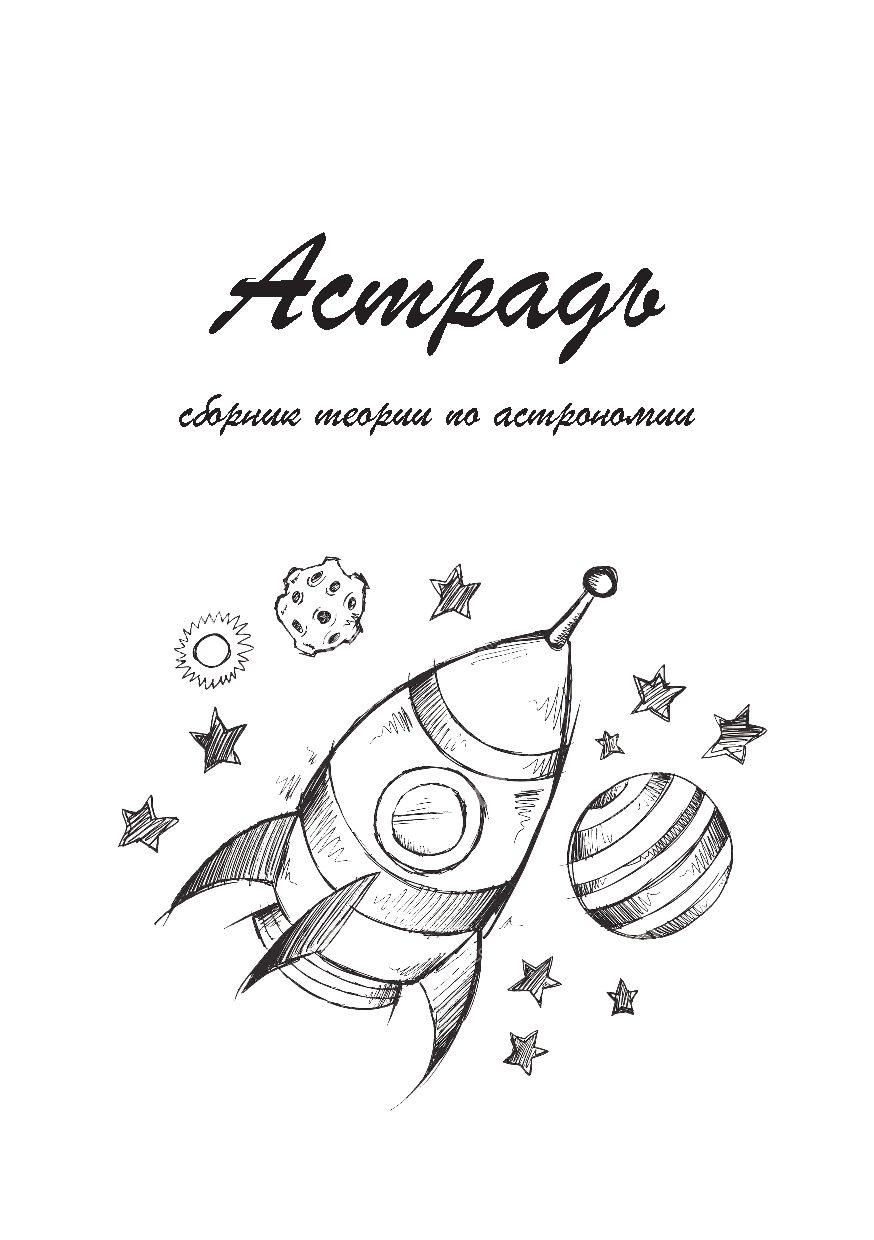
\includegraphics[width=0.95\tw]{sys/cover.pdf}\\[1pc]
{\scshape Beograd, Srbija \\ \year}	
\end{center}

%	\thispagestyle{empty}
\begin{center}
	{\sffamily \large А.\,С.~Шепелев, Д.\,А.~Долгов, С.\,Д.~Молчанов, С.\,Б.~Борисов}\\[-7pt]
	
	\rule{0.88\tw}{0.7pt} \\[12pc]

	
	
	\scalebox{2}{\Huge \bfseries \scshape Астрадь}\\[1pc]
	{\Large \scshape краткий сборник теории\\[.5pc] по астрономии}\\[4pc]
	\vfill
	{\scshape Астрономический кружок\\ им.~Е.\,П.~Левитана}
	\vfill
	{\scshape Жуковский \\ 2018}
\end{center}
	\newpage
\setcounter{page}{2}
\thispagestyle{empty}
	\noindent ББК 22.6\\
%	\hspace*{1.8pc} 
	A 91\\
	УДК 52\\[1pc]

{\small {\itshape Рецензент:}\\ учитель астрономии М.\,В.~Кузнецов (МОУ Гимназия №1~~г.\,о.~Жуковский)}\\[1pc]

{\small {\itshape Редакторы:}\\ 
выпускник Московского государственного университета А.\,В.~Афанасьев,\\
магистр политехнического института Гренобля, бакалавр Московского физико-тех\-ни\-чес\-кого института В.\,А.~Сушко\\[1pc]}


{%\hspace{1pc} 
{\bfseries А.\,С.~Шепелев, Д.\,А.~Долгов, С.\,Д.~Молчанов, С.\,Б.~Борисов}\\ Астрадь~--- краткий сборник теории по астрономии. 2020.~---~64~с: 2-е изд. ISBN 978-5-9909877-1-5\\[2pc]

{\small Астрадь является учебным пособием по астрономии, рекомендованным для школьников 7\,--\,11 класса. Сборник составлен неоднократными призерами международных олимпиад по астрономии, членами астрономического кружка им.~Е.\,П.~Левитана г.\,о.~Жуковский. 

Здесь читатель сможет найти необходимый минимум теории для участия в различных олимпиадах школьников по астрономии. Также Астрадь можно использовать и для освоения школьной программы, потому что наряду со сложными темами освещены и самые базовые вопросы астрономии.}\\[1pc]

{\small{\itshape Вёрстка:} А.\,С.~Шепелев}\\ \vfill


\noindent\begin{minipage}[t]{0.4\tw}
	{\bfseries ISBN 978-5-9909877-1-5}
\end{minipage}
\hfill
\begin{minipage}[t]{0.57\tw}
	\small
	\copyright\,А.\,С.~Шепелев, Д.\,А.~Долгов,\\
	 \hspace*{8pt} С.\,Д.~Молчанов, С.\,Б.~Борисов, 2018\\[3pt]
	\copyright\,Астрономический кружок\\ \hspace*{8pt} им.~Е.\,П.~Левитана г.\,о.~Жуковский, 2018
\end{minipage}
\newpage
	\setcounter{tocdepth}{2}
	{
		\small 
		\renewcommand{\baselinestretch}{ 0.95 } 
		\tableofcontents 
		\label{toc}
		\renewcommand {\baselinestretch}{ 1.02 }
	}
	\newpage
	\section{Небесная механика}
\subsection{Расстояние и размеры}
\term{Астрономическая единица}~--- единица измерения расстояния в астрономии, 
равная большой полуоси орбиты Земли.\begin{equation}
	1~\au = 149\:597\:870\:700~\text{м} \simeq 1.5 \times 10^{11}~\text{м}.
\end{equation}

\term{Годичный параллакс} ($\pi$) объекта~--- это угол, под которым видно 
орбиту Земли из окрестностей данного объекта. Применяется к объектам вне 
Солнечной системы. \begin{equation}
	\tg \pi = \frac{a_\oplus}{r},
	\label{eq:parallax-sin}	
\end{equation}
где $a_\oplus$~--- большая полуось орбиты Земли и $r$~--- расстояние до объекта 
имеют одинаковые единицы измерений. Учитывая малость угла $\pi$, можно считать $\tg\pi \simeq \pi$ в \eqref{eq:parallax-sin}, тогда
\begin{equation}
	\pi = \frac{a_\oplus}{r}.
	\label{eq:parallax}
\end{equation} 
\begin{figure}[h!]
	\centering
	\vspace{-1pc}
	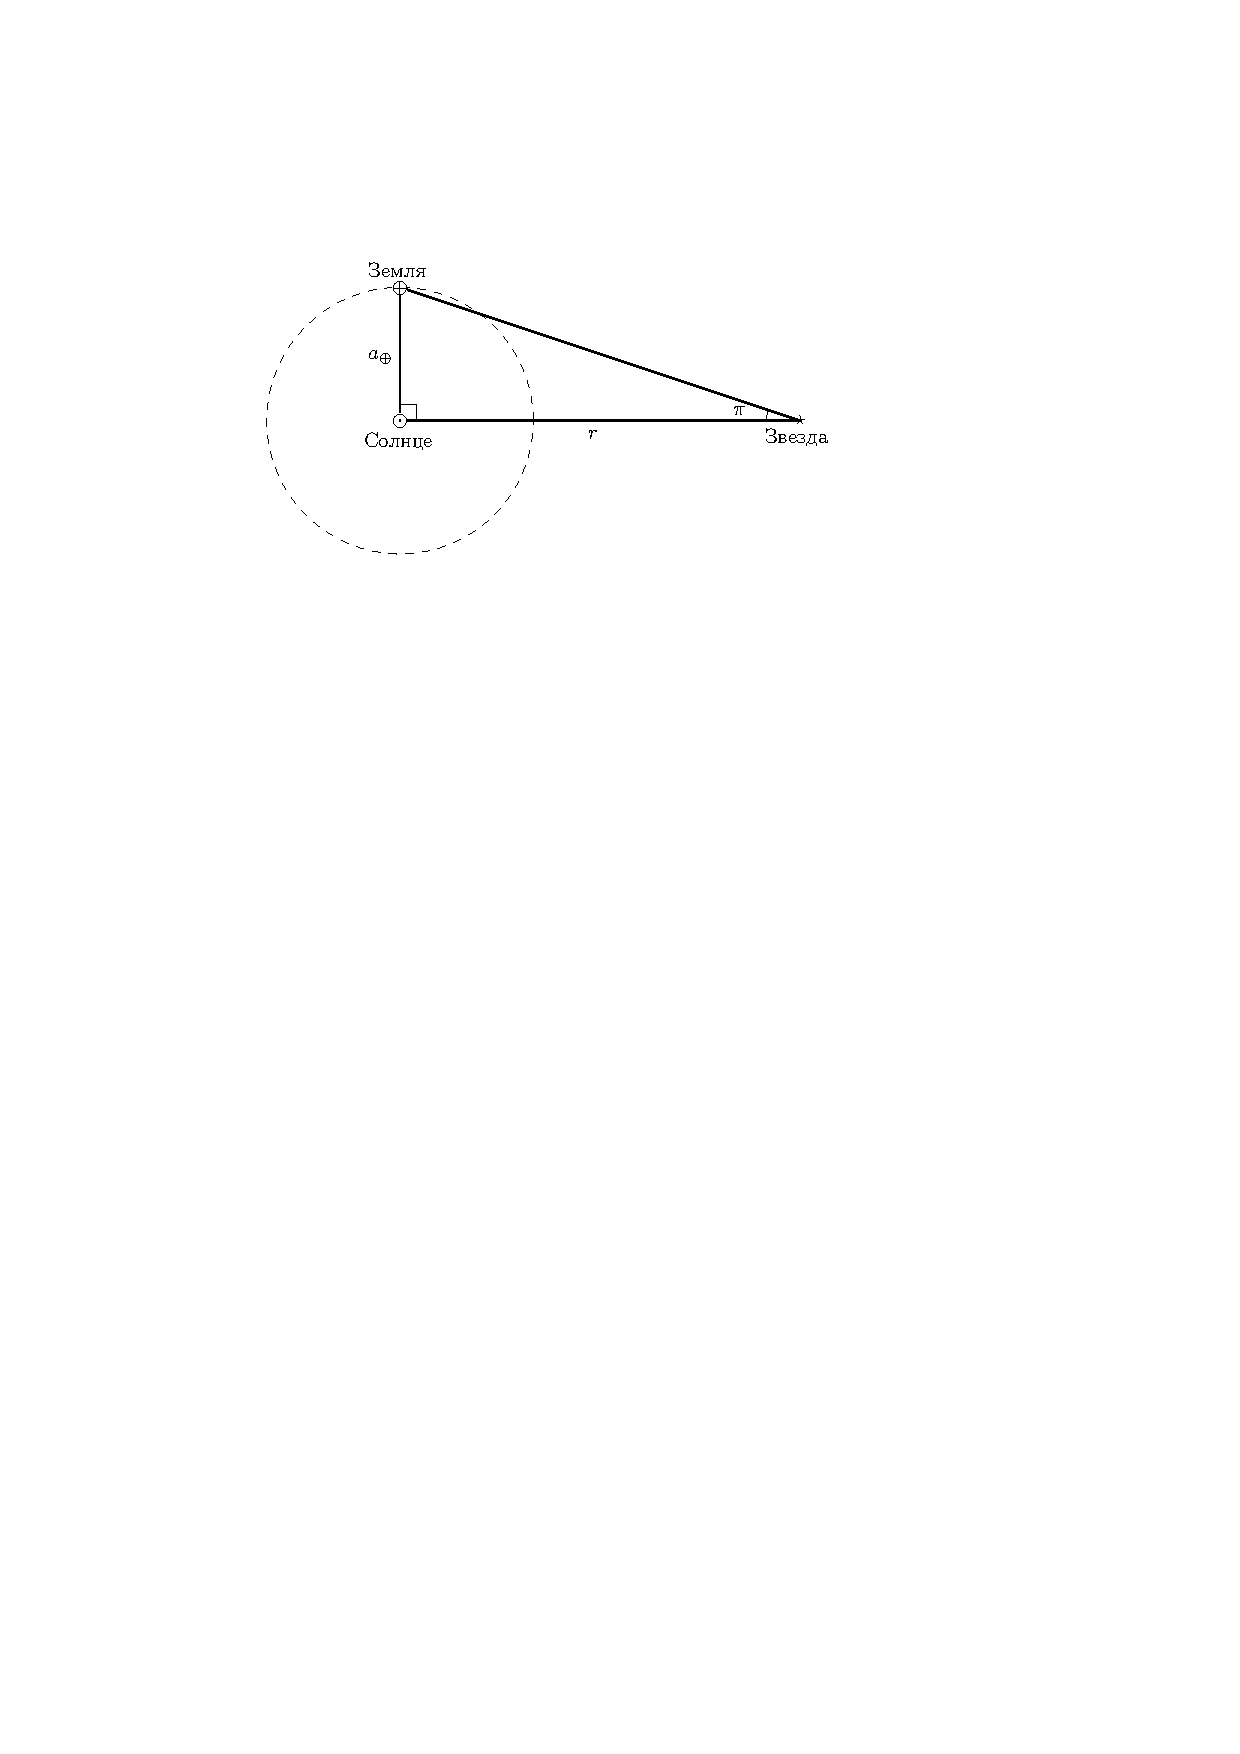
\includegraphics[width = 0.7\tw]{parallax.pdf}
	\caption{Схема годичного параллакса}
\end{figure}

Расстояние $r$, с которого большая полуось орбиты Земли $a_\oplus$ видна под углом $\pi = 1''$ называется \term{1 парсеком}. Так как \begin{equation}
	1~\text{рад} = \frac{180^\circ}{\pi} \simeq  3 438' \simeq 206265'' 
\quad \Longrightarrow \quad \mathsf{1~\text{\sffamily пк} = 
206265~\text{\sffamily а.\,е.}},
\end{equation} 
следовательно, записывая большую полуось орбиты Земли в \au, а расстояние до звезды в парсеках, получаем параллакс в секундах. Таким образом,
\begin{equation}
	r_\text{пк} = \frac{1~\au}{\pi''}.
\end{equation}

\term{Угловой размер объекта}~--- это угол, под которым видно объект. Для сферически симметричных объектов с радиусом $R$, угловой размер (диаметр) при наблюдении с расстояния $r$ определяется как
\begin{equation}
\rho = 2 \arcsin \frac{R}{r}.
\end{equation}
В случае, когда $r\gg R$, можно считать, что $\sin \rho \simeq \rho$, тогда
\begin{equation}
	\rho \simeq \frac{2 R}{r}.
\end{equation}

\vspace{-1.5pc}
\begin{figure}[h!]
	\begin{minipage}[b]{0.5\tw}
		\begin{flushleft}
			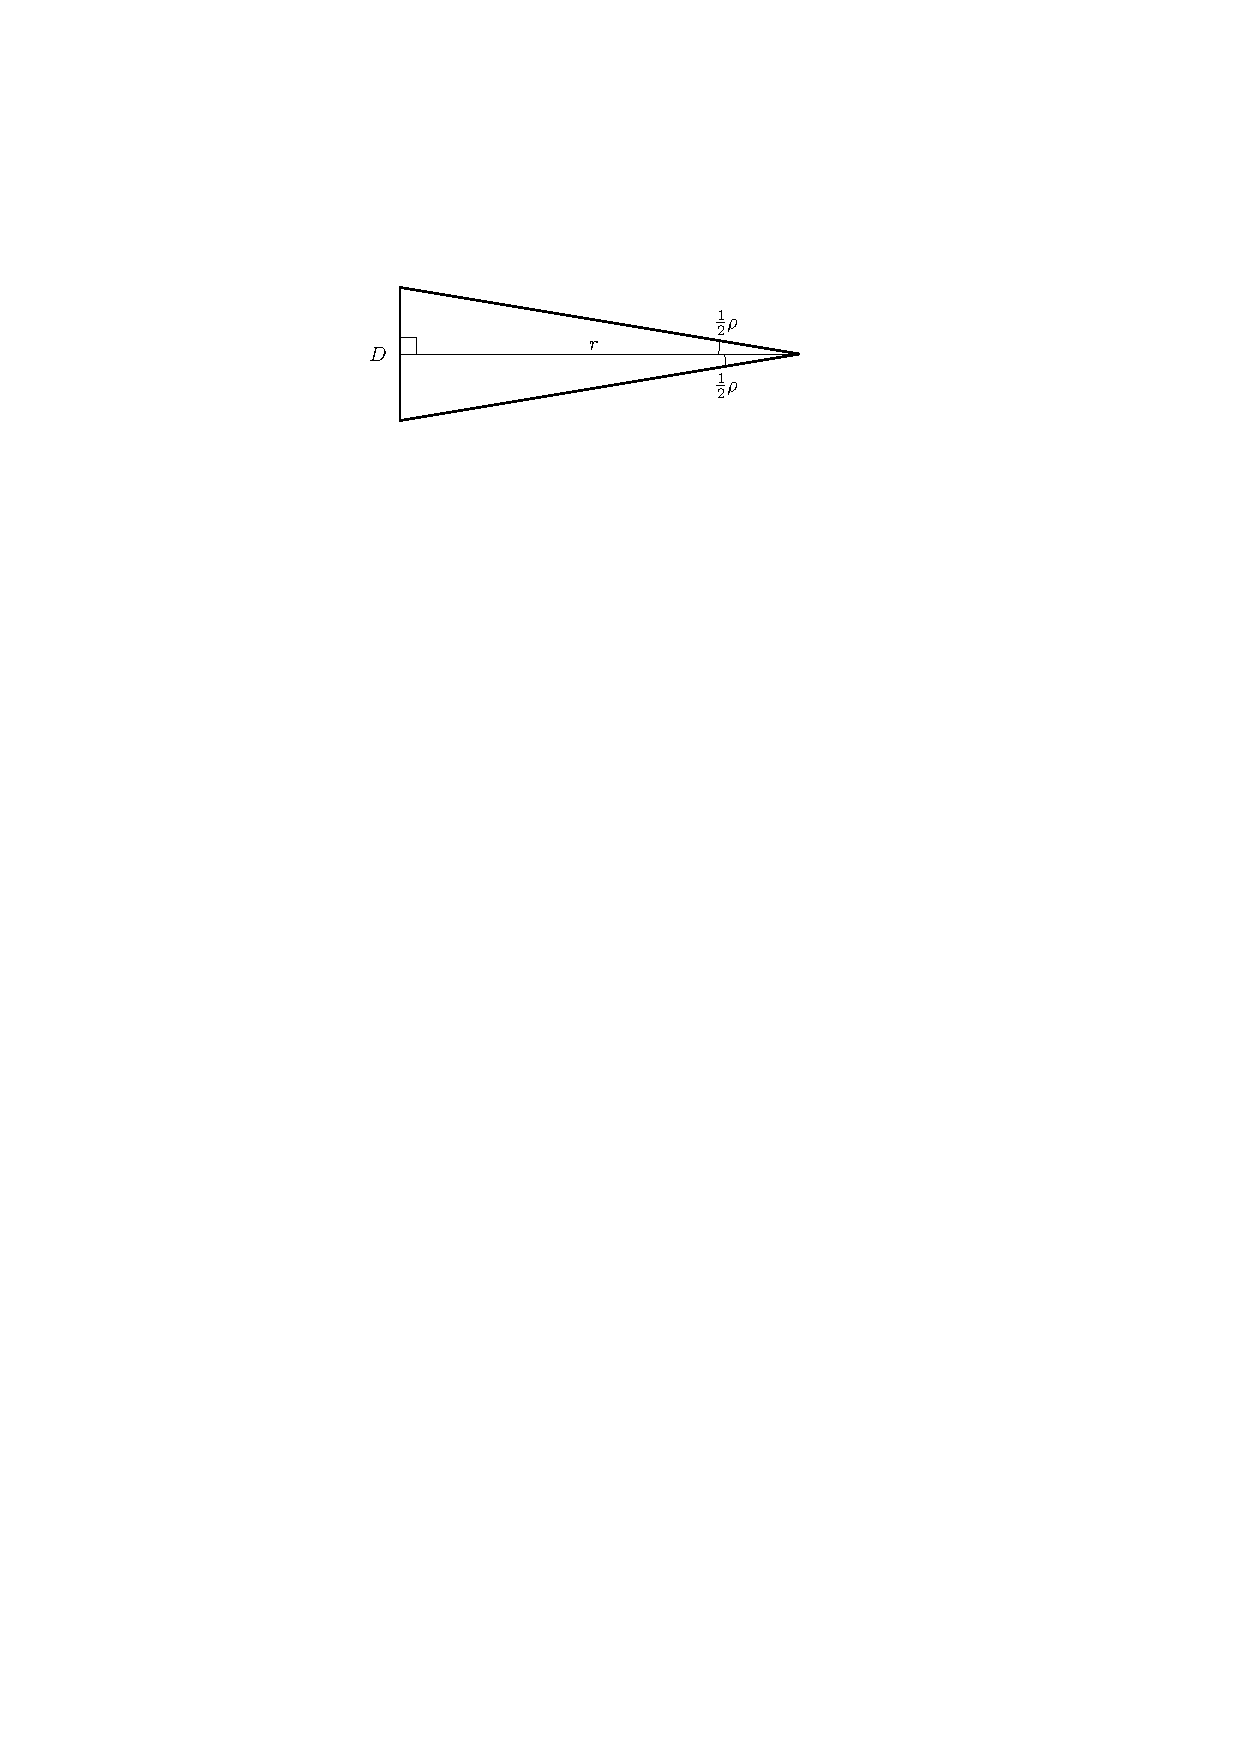
\includegraphics[width = 0.93\tw]{angle-size}
			\captionof{figure}{Угловой размер}
		\end{flushleft}
	\end{minipage}
	\begin{minipage}[b]{0.5\tw}
		\centering
		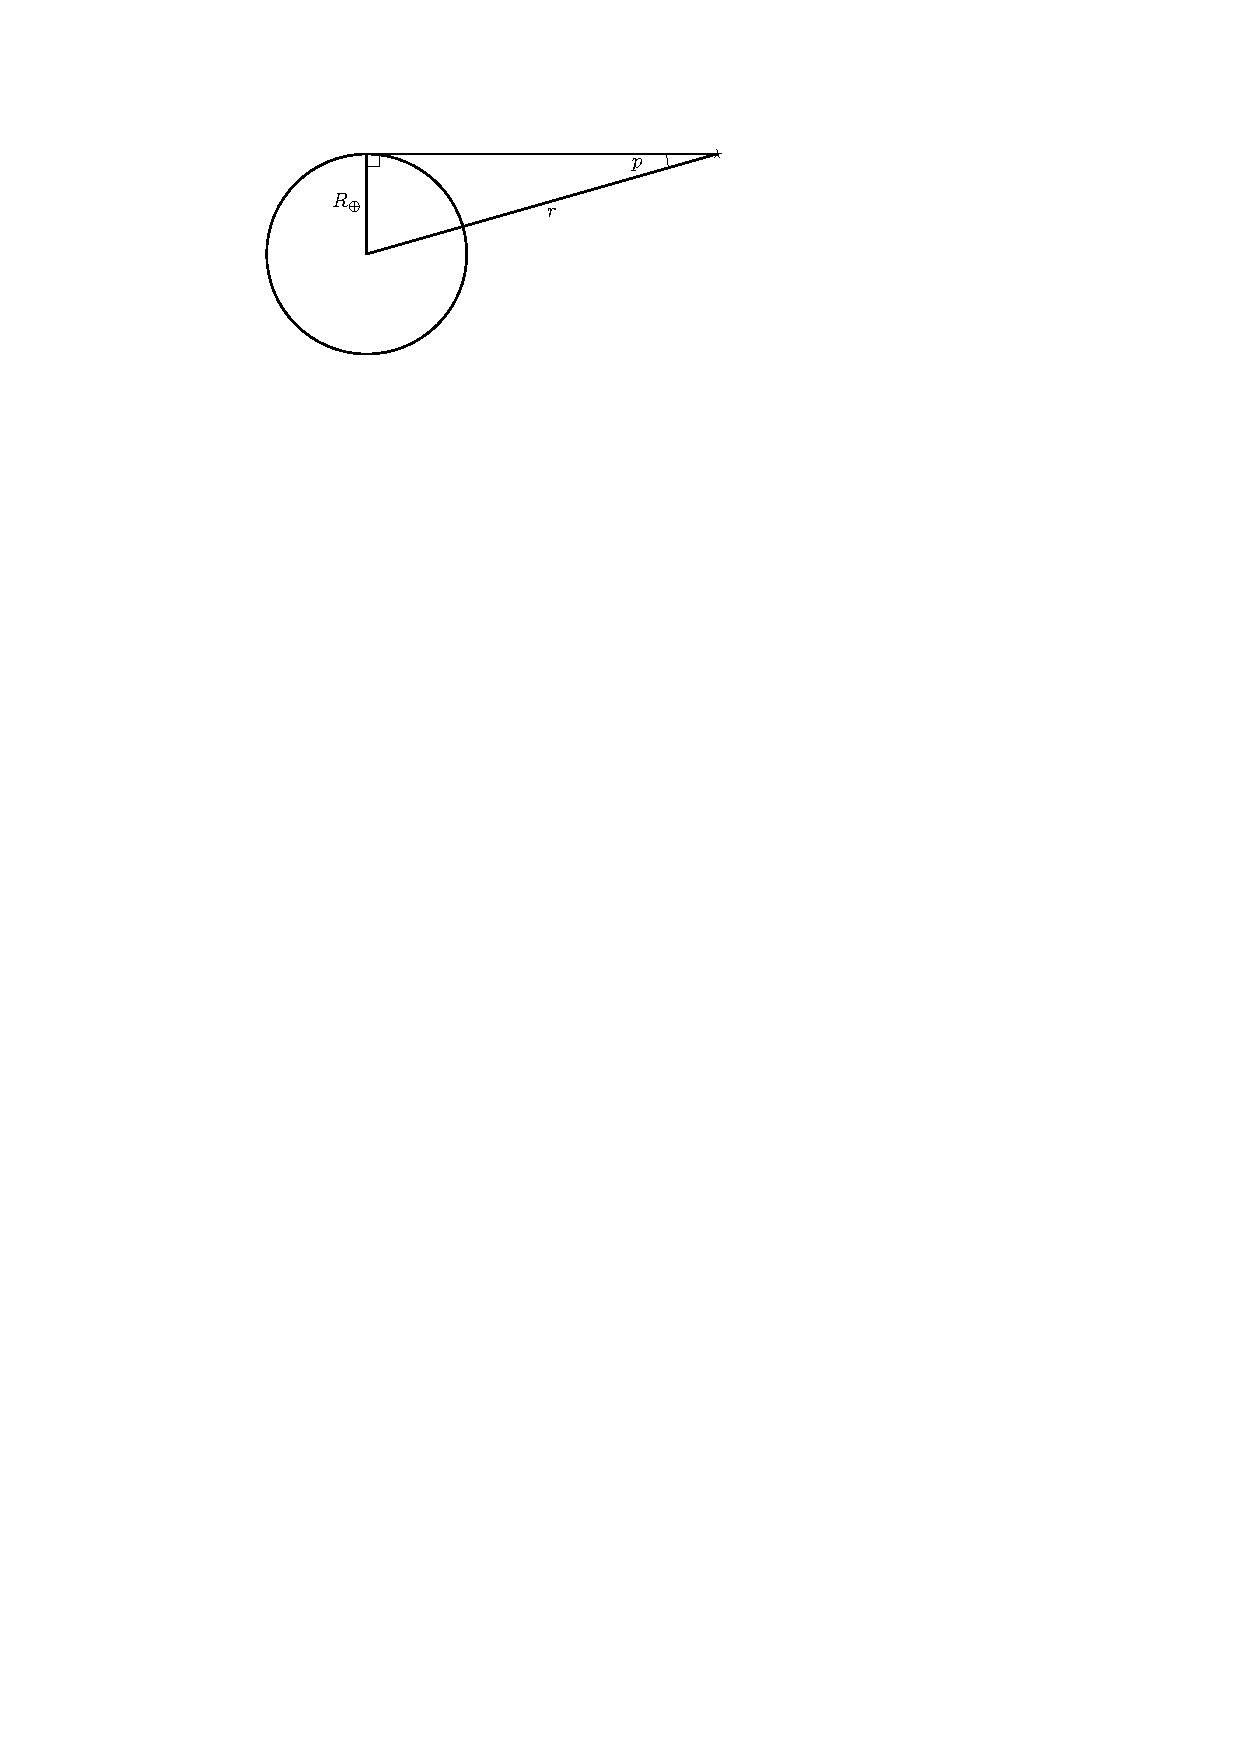
\includegraphics[width = \tw]{parallax-horiz}
		\captionof{figure}{Горизонтальный параллакс}
	\end{minipage}
\end{figure}

\term{Горизонтальный параллакс}~$(p)$~--- это угол, под которым виден радиус Земли~$R_\oplus$ для наблюдателя в центре объекта, когда последний находится на горизонте:
\begin{equation}
\sin p=\frac{R_\oplus}{r}.
\end{equation}

\term{Правило Тициуса-Боде} --- эмпирическая формула, приблизительно описывающая 
радиусы орбит планет в Солнечной системе:
\begin{equation}r=\frac{3\cdot 2^n+4}{10}, \quad n=-\infty, 0, 1, 2...
\end{equation}


\subsection{Закон всемирного тяготения}
Согласно \imp{закону всемирного тяготения}, сила притяжения 
между двумя точечными телами с массами $M$ и $m$,
находящимися на расстоянии $r$, равна
\begin{equation}
	F=\frac{GMm}{r^2}, \label{eq:grav-law}
\end{equation}\nopagebreak где $G\simeq 6.67\cdot 10^{-11}~\text{м}^3 / 
\left( \text{кг} \cdot \text{с}^2 \right)$~--- 
\term{гравитационная постоянная}.

\term{Гравитационный потенциал} поля точечной (или сферически 
симметричной) массы $M$ на расстоянии $r$ от нее равен
работе, которую необходимо затратить, чтобы принести
единичную массу с бесконечности в данную точку. Так как
гравитационные силы между двумя массами --- это силы 
притяжения, то эта работа отрицательна. Данная
величина также является \term{потенциальной энергией} точечной
массы на расстоянии $r$ от массы $M$, а выражение для нее имеет 
следующий вид:\begin{equation}
U=-\frac{GM}{r}.
\end{equation}

Напряженность гравитационного поля $dU/dr$ часто называют 
\term{ускорением свободного падения} $g$, она вычисляется по формуле
\begin{equation}
	g = \frac{GM}{r^2}.
	\label{eq:g}
\end{equation}
Тогда (\ref{eq:grav-law}) можно записать как \begin{equation}
	F = mg.
\end{equation}

\subsection{Закон сохранения энергии и типы орбит}
Для движения тела c массой $m$ в гравитационном  в поле тела
с массой \linebreak $M\gg m$ со скоростью $v$ на расстоянии $r$ от
гравитационного центра справедливо следующее соотношение:
\begin{equation}
	\frac{m v^2}{2}-\frac{GM m }{r}=E_0,
\end{equation}
где $E_0$~--- величина, равная сумме кинетической и потенциальной энергии тела. Она постоянна, если на тело не действуют внешние силы, кроме силы притяжения к центральному телу. Данное равенство принято называть \term{законом сохранения энергии} для тела, движущегося в поле консервативных (потенциальных) сил.

\begin{wrapfigure}[10]{l}{.5\tw}
	\centering
	\vspace{-1pc}
	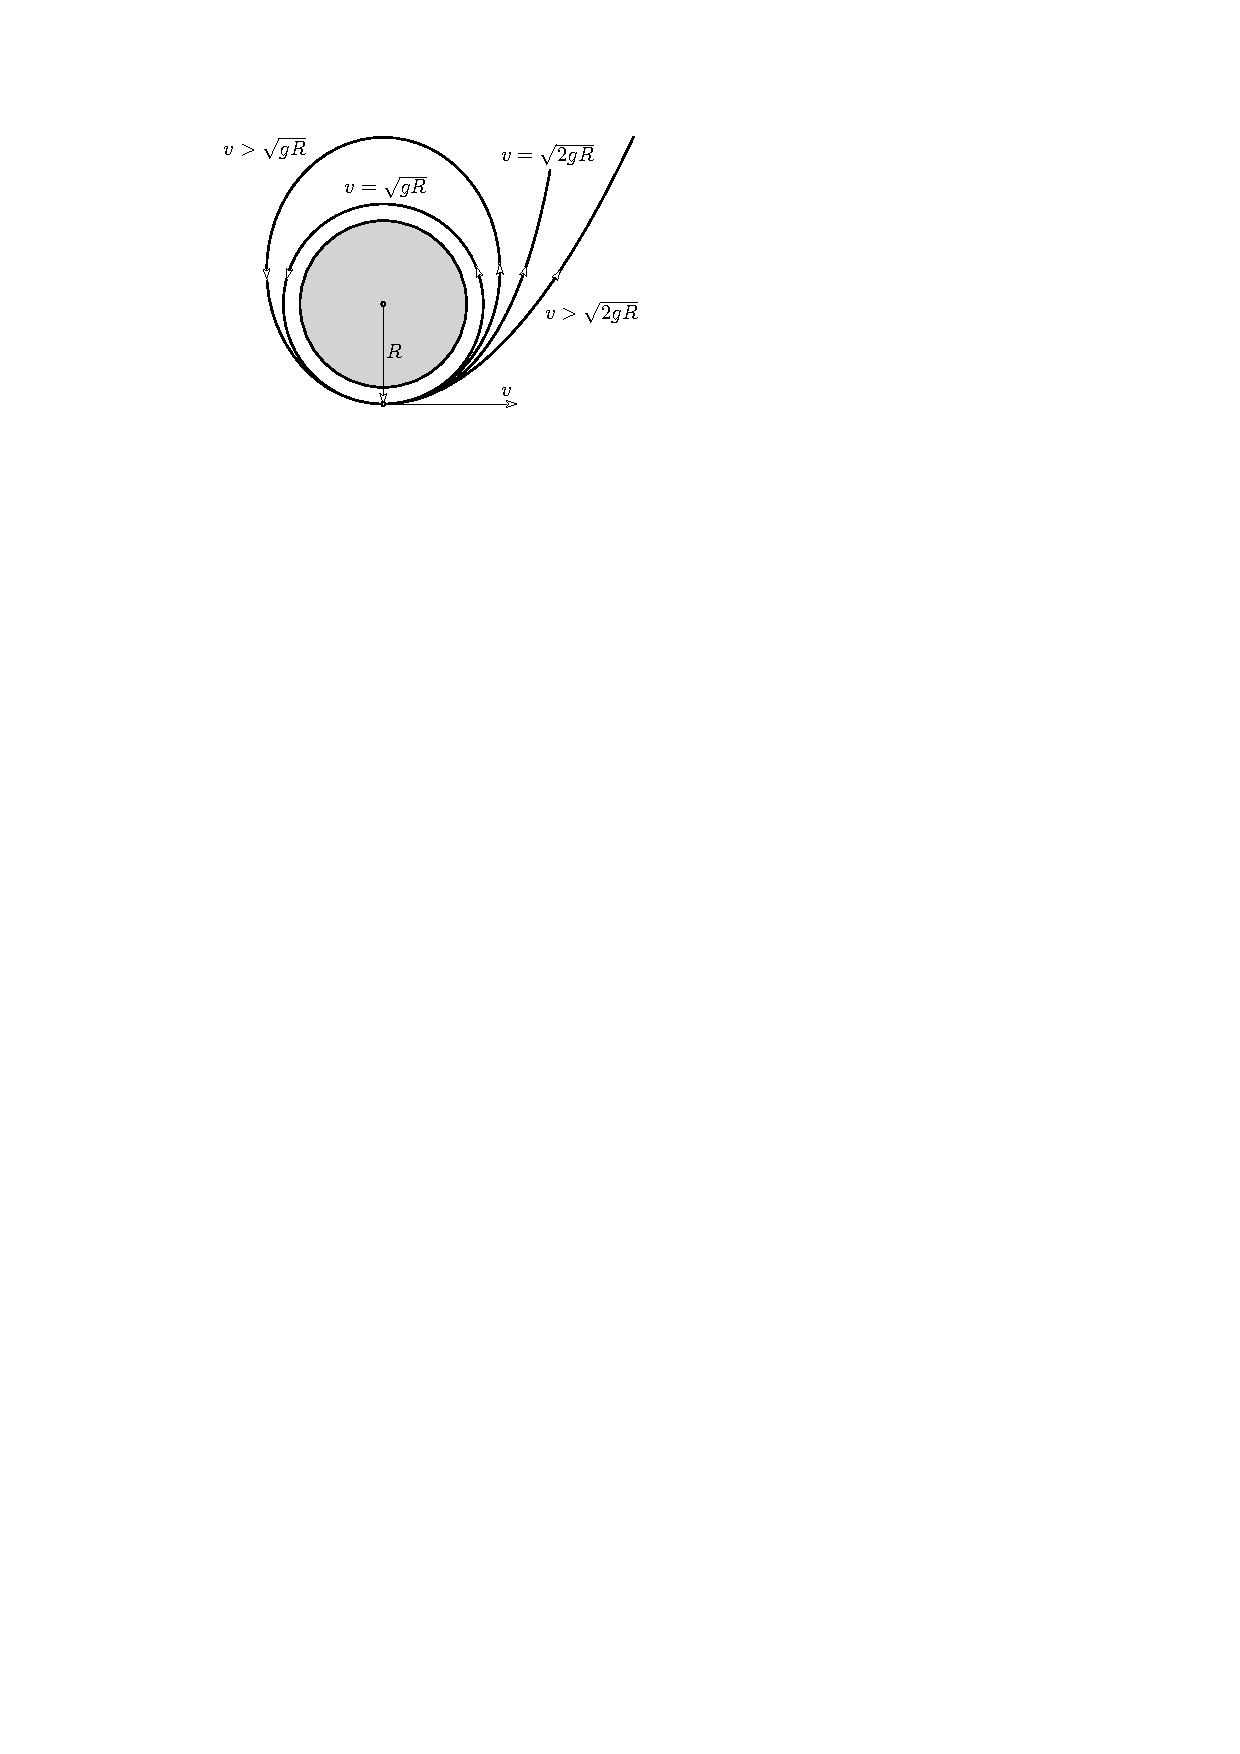
\includegraphics[width = 0.45\tw]{speeds}
	\caption{Возможные траектории тела \label{pic:orbits}}
\end{wrapfigure}
Если $E_0>0$, то траектория тела~--- \imp{гипербола},
ветви которой асимптотически приближаются к двум прямым. Стоит заметить,
что на бесконечно большом удалении малого \linebreak тела от массивного
его скорость остается положительной, так как суммарная энергия $E_0$
больше нуля.

Если $E_0=0$, то траектория тела~--- \imp{парабола}. При стремлении
расстояния $r$ между телами к бесконечности скорость тела с стремится к нулю.

Отсюда становится очевидно, что при параболической и гиперболической
траекториях движение тела не ограничено (инфинитно).

Если $E_0<0$, то траектория тела~--- \imp{эллипс}. При
эллиптической траектории движение ограничено (финитно), так как малое тело
не может бесконечно удаляться по причине того,
что суммарная энергия меньше нуля.

На Рис.\,\ref{pic:orbits} представлены примеры возможных траекторий малого тела
относительно центрального (точка C). При $v_0 > v_{2}$ тело движется
по гиперболе, при $v_0 = v_{2}$~--- по параболе,
а при $v_0 < v_{2}$~--- по эллипсу.

\term{Первая космическая скорость} --- минимальная скорость, необходимая для
того, чтобы маломассивное тело стало искусственным спутником центрального тела.
\begin{equation}v_1=\sqrt{\frac{GM}{R}},
\end{equation}
где $M$ --- масса центрального тела, а $R$~--- радиус орбиты. Отсюда несложно получить выражение для
скорости искусственного небесного тела на высоте~$h$ над~поверхностью тела радиуса $r_0$:
\begin{equation}
	v_h=\sqrt{\frac{GM}{r_0+h}}=\sqrt{\frac{g r_0^2}{r_0+h}}.
\end{equation}

\begin{wrapfigure}[10]{r}{.5\tw}
	\centering
	\vspace{-1pc}
	a	\caption{Движение по окружности \label{pic:orb-vel}}
\end{wrapfigure}
\change{Вывод:
\\
Рассмотрим 2 точки из траектории ($А$ и $В$) и скорости объекта в этих точках ($v_A$ и $v_B$) соответственно.
\begin{equation}
	\vec{\Delta v} = \vec{v_B} - \vec{v_A}
\end{equation}
При устремлении промежутка времени между пунктами к 0 можно считать, что длина пути становится равна длине хорды $AB$.
\begin{equation}
	\alpha = \frac{\Delta v}{v_A} = \frac{AB}{R}.
\end{equation}
Посчитаем модуль среднего ускорения:
\begin{equation}
	\langle a \rangle = \frac{\Delta v}{\Delta t} = \frac{v \Delta l}{R \Delta t}.
\end{equation}
Перейдя к пределу, получим мгновенное ускорение
\begin{equation}
	a = \lim_{\Delta t \rightarrow 0} \langle a \rangle = \lim_{\Delta t \rightarrow 0} \frac{v \Delta l}{R \Delta t} = \frac{v}{R} \lim_{\Delta t \rightarrow 0} \frac{\Delta l}{\Delta t} = \frac{v^2}{R}.
\end{equation}
Отсюда получаем значение для круговой скорости:
\begin{equation}
	v = \sqrt{a R} = \sqrt{\frac{G M}{R}}.
\end{equation}
}

\term{Параболическая} или \term{вторая космическая скорость} ---
минимальная скорость, необходимая для того, чтобы маломассивное тело преодолело гравитационное притяжение центрального тела, стартуя с расстояния $r$ от его центра масс, и покинуло замкнутую орбиту вокруг
последнего. Выражение для нее имеет следующий вид:
\begin{equation}
	v_{2}=\sqrt{\frac{2GM}{r}}.
\end{equation}
Для стабильной системы, частным случаем которой является тело на круговой орбите, справедлива
\term{теорема о вириале}:
\begin{equation}
	2 \langle T\rangle
	= -\sum _{{k=1}}^{N}\langle (\vec{F}_{k}, \vec{r}_{k})\rangle
	= -\langle \Pi \rangle,
\end{equation}
где $\langle T\rangle$ --- средняя полная кинетическая энергия, $\vec{F}_k$~--- сила,
действующая на $k$-ю частицу, $\vec{r}_k$~--- радиус-вектор $k$-й частицы. Другими словами, удвоенная средняя полная
кинетическая энергия $T$ равна средней полной потенциальной энергии $\Pi$ со знаком минус. Применяя теорему о вириале для тела, обращающегося по круговой орбите, можно
получить выражение для первой космической скорости.

\subsection{Законы Кеплера}
\term{I-ый закон:} Все планеты движутся по
эллиптическим орбитам, в одном из фокусов которых
находится Солнце.\\

\term{ II-ой закон:} Радиус-вектор планеты за
равные промежутки времени заметает равные площади:
\begin{equation}
	\frac{dS}{dt}=\const = \frac{S_\text{элл}}{T} = \frac{\pi a b }{T}.
\end{equation}
\term{III-ий закон:} Квадраты периодов обращения планет
относятся как кубы больших полуосей их орбит.
\begin{equation}
	\frac{T^2_1}{T^2_2}=\frac{a^3_1}{a^3_2},
\end{equation}
где $a$ --- большая полуось, $T$ --- период обращения.
\begin{figure}[h!]
	\begin{minipage}[b]{0.5\textwidth}
		\centering
		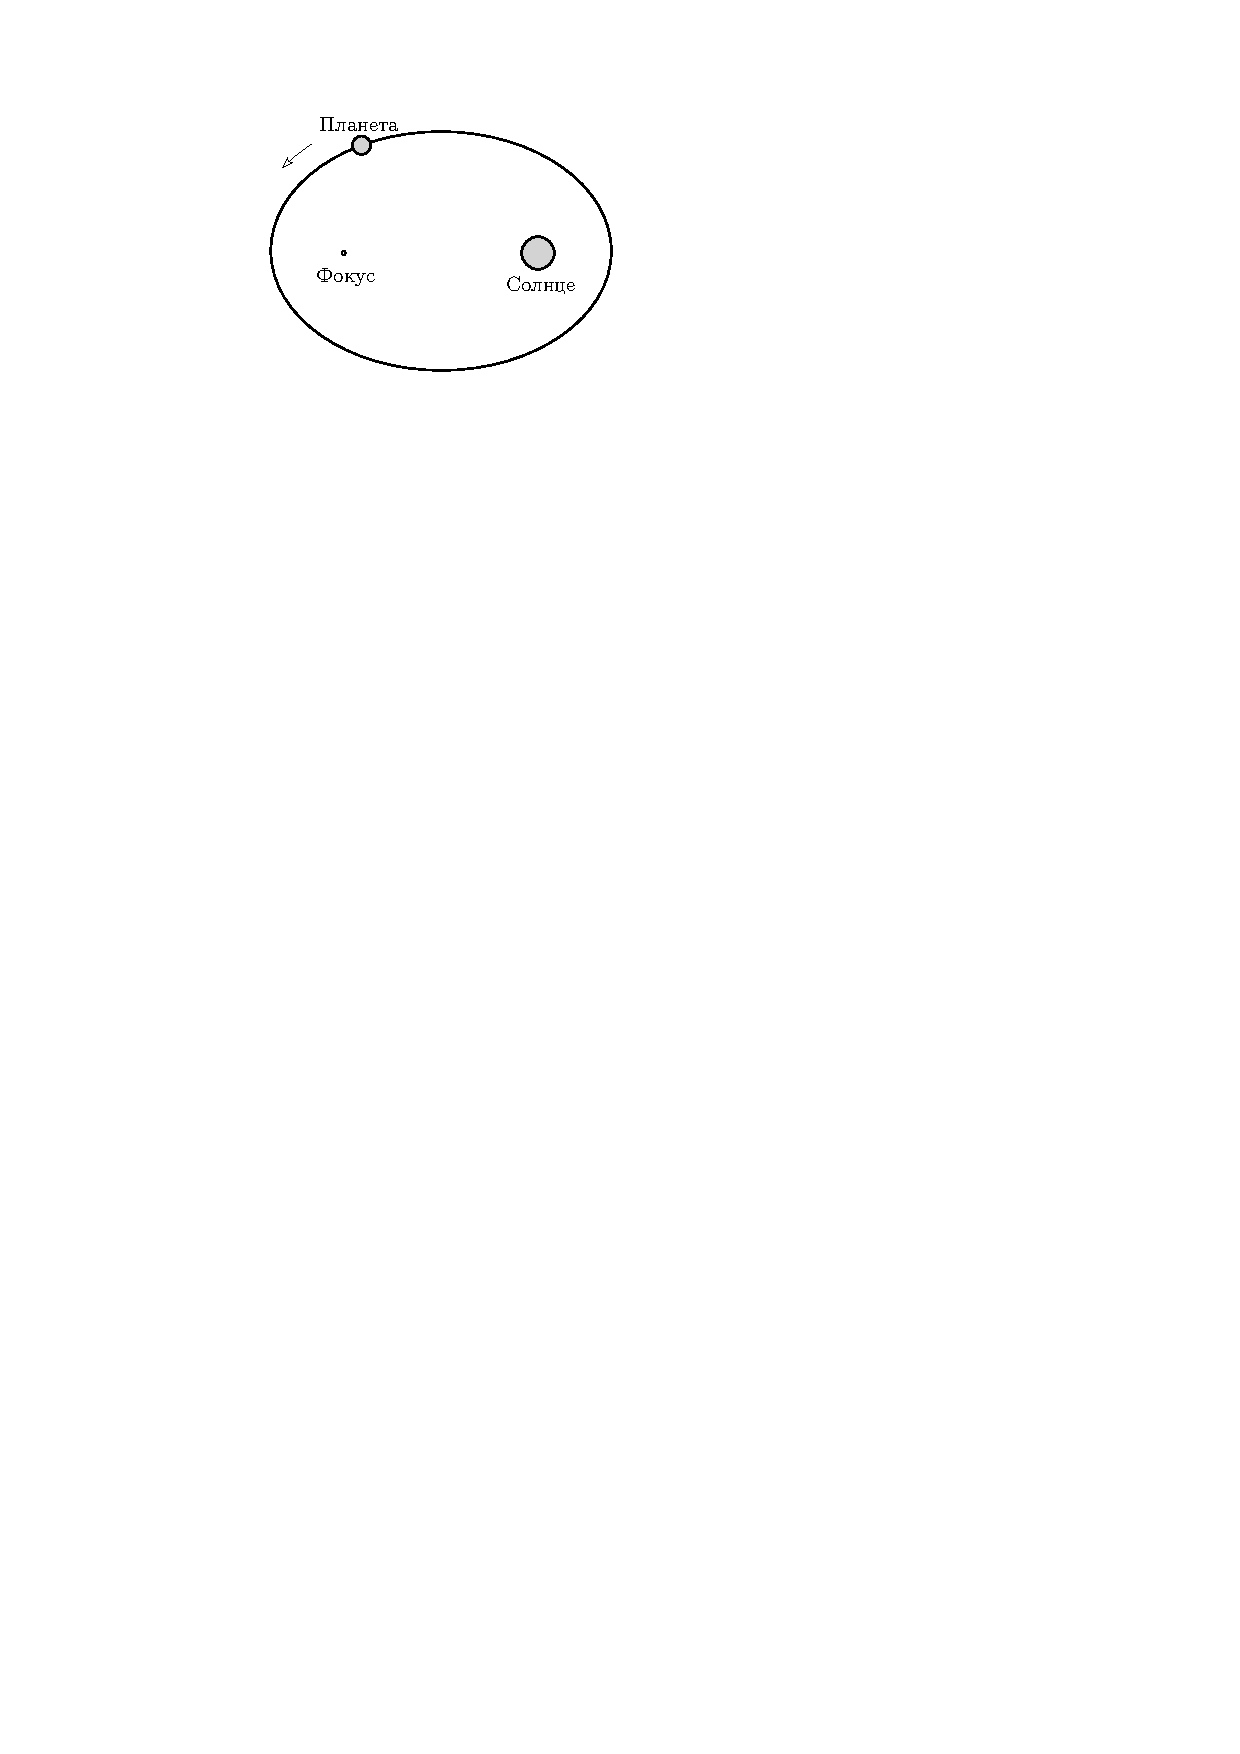
\includegraphics[width = 0.84\textwidth]{first-kepler}
		\caption{Первый закон Кеплера}
	\end{minipage}
	\begin{minipage}[b]{0.5\textwidth}
		\centering
		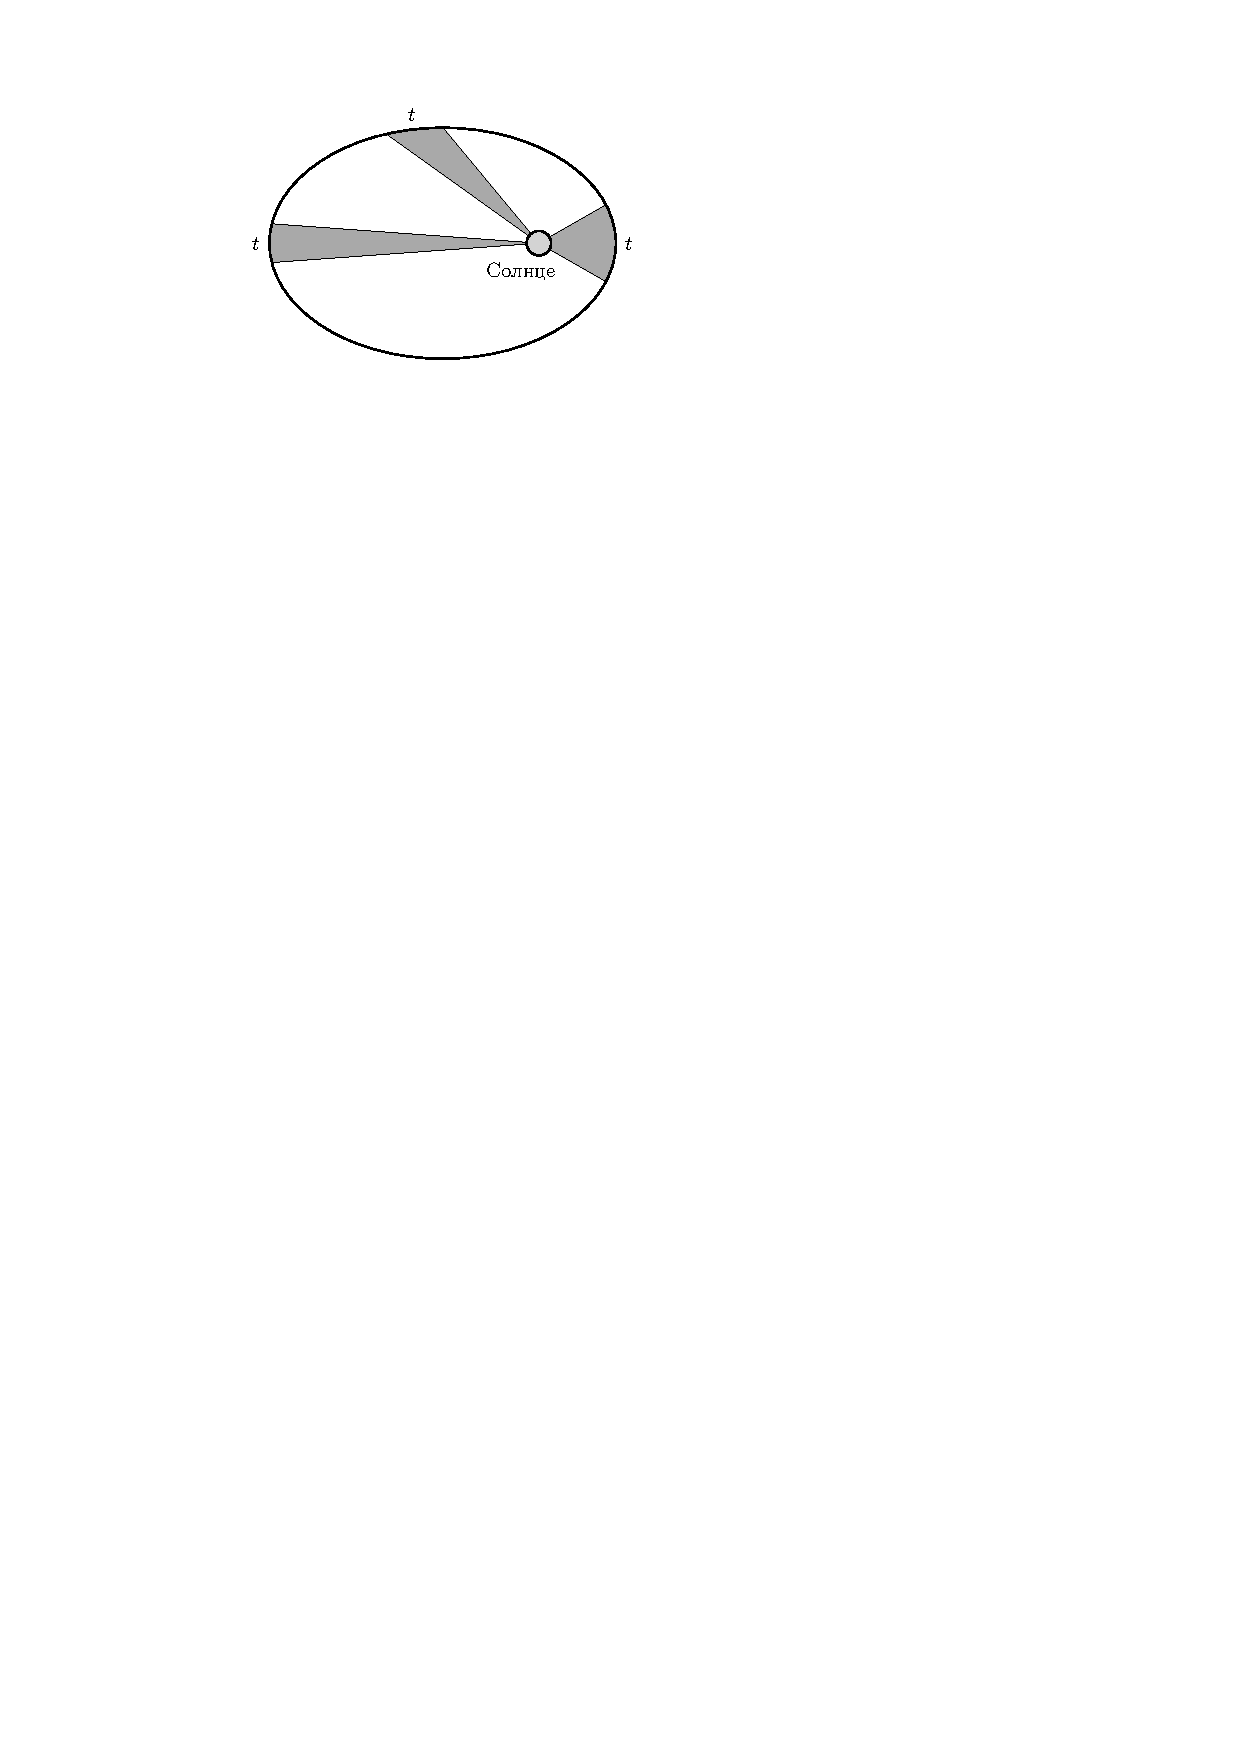
\includegraphics[width = 0.972\textwidth]{second-kepler}
		\caption {Второй закон Кеплера}
	\end{minipage}
\end{figure}

\term{Обобщённый} Ньютоном \term{III-ий закон Кеплера} имеет следующий вид:
\begin{equation}
	\frac{T^2_1( M_1 + m_1)}{T^2_2( M_2 + m_2 )}=\frac{a^3_1}{a^3_2} \quad \Longleftrightarrow \quad
	\frac{T^2 ( M + m )}{a^3} = \frac{4 \pi^2}{G},
\end{equation}
где $M_1$ и $M_2$~--- массы центральных тел, $m_1$ и
$m_2$~--- массы обращающихся вокруг них тел. Так как массы планет
$m$ много меньше массы звезды $M$, $M + m \simeq M$.

\subsection{Движение по орбите}
\begin{figure}[t]
	\centering
	\begin{tikzpicture}
		\footnotesize
		
		%	\foreach \x in {0, .1,...,5} {
		%		\draw [line width=.1pt] (\x, -3) -- (\x, 3);
		%	};
		%
		%	\foreach \y in {-3, -2.9,...,3} {
		%		\draw [line width=.1pt] (0, \y) -- (5, \y);
		%	};
		
		\draw [thick] (0, 0) .. controls (2, 4) and (3, -1) .. (5, -1);
		\draw [-latex] (0, -2) -- (1.25, 1.5);
		\draw [-latex] (0, -2) -- (3.3, .1);
		\draw [-latex] (1.25, 1.5) -- (3.3, .1);
		
		\draw (.3, -1.8) arc(31:70:0.36);
		
		\draw (.6, -.3) node [anchor = east] {$\vec{r}(t)$};
		\draw (1.6, -.9) node [anchor = north west] {$\vec{r}(t + dt)$};
		\draw (2.3, 0.9) node [anchor = north east] {$d\vec{r}$};
		\draw (0.2, -1.5) node [anchor = south west] {$\boldsymbol{\omega} \,dt$};
		
		\draw[fill=white] (1.25, 1.5) circle (0.03);
		\draw[fill=white] (3.3, .1) circle (0.03);
		\draw[fill=white] (0, -2) circle (0.03);
		
	\end{tikzpicture}
	\caption{}
\end{figure}

Рассмотрим такую физическую величину, как \term{секториальная скорость}~--- это векторная величина, описывающая ориентированную площадь, заметаемую радиус вектором тела за единицу времени. Пусть в момент времени $t$ тело находилось в точке $\vec{r}(t)$, а через промежуток времени $dt$~--- в точке $\vec{r}(t + dt)$. Обозначим перемещение тела за этот промежуток времени как $d\vec{r}$. Его можно выразить через скорость тела в момент времени $t$, считая ее постоянной на промежутке от $t$ до $t + dt$: $d\vec{r} = \vec{v} \, dt$. Площадь, которую заметает радиус-вектор тело $\vec{r}(t)$ равна половине параллелограмма, построенного на векторах $\vec{r}(t)$ и $d\vec{r}$. Поэтому можно записать
\begin{equation*}
	\vec{s} = \frac{1}{2} [\vec{r} \times \vec{v} dt],
\end{equation*}
следовательно секториальная скорость равна
\begin{equation*}
	\boldsymbol{\sigma} = \frac{d \vec{s}}{dt} = \frac{1}{2} [\vec{r} \times \vec{v}] = \frac{\vec{l}}{2} = \frac{\vec{L}}{2m},
\end{equation*}
где $\vec{l}$~--- удельный момент импульса (на единицу массы). Полученное выражение доказывает \imp{второй закон Кеплера}.

С другой стороны, перемещение $d\vec{r}$ можно выразить через угловую скорость $\boldsymbol{\omega}$, как $d \vec{r} = [\vec{r} \times \boldsymbol{\omega}\,dt]$. Тогда
\begin{equation*}
	\boldsymbol{\sigma}
	= \frac{1}{2} \big[ \vec{r} \times [\vec{r} \times \boldsymbol{\omega} ]\big]
	= \vec{r} \underbrace{(\vec{r}, \boldsymbol{\omega})}_0 - \boldsymbol{\omega} ( \vec{r}, \vec{r} )
	= r^2 \boldsymbol{\omega}.
\end{equation*}
Получим \imp{третий закон Кеплера}, заметив, что модуль секториальной скорости можно записать, как
\begin{gather*}
	\sigma
	= \frac{S_\text{эл}}{T}
	= \frac{\pi a b}{T}
	= \frac{L}{2m},\\
	\frac{\pi a^2 \sqrt{1 - e^2}}{T}
	= \frac{m \sqrt{\dfrac{GM}{a} \cdot \dfrac{1 + e}{1 - e}} \cdot a(1-e)}{2m},\\
	\frac{4\pi^2 a^4 (1 - e^2)}{T^2}
	= a^2(1-e)^2 \cdot \frac{GM}{a} \cdot \frac{1 + e}{1-e}
\end{gather*}
\begin{equation}
	\frac{T^2}{a^3} = \frac{4\pi^2}{GM}.чч
\end{equation}

Получим еще одно важное соотношение~--- \term{интеграл энергии}~--- формулу для скорости тела на орбите с большой полуосью $a$ в точке, удалённой на расстояние~$r$ от центрального тела с массой $M$. Для этого рассмотрим  сначала точку перицентра ($q$, <<п>>) и апоцентра ($Q$, <<a>>) данной орбиты, запишем для них закон сохранения энергии и закон сохранения момента импульса:
\begin{gather*}
	-\frac{GMm}{q} + \frac{m v^2_\text{п}}{2} = -\frac{GMm}{Q} + \frac{m v^2_\text{а}}{2},\\
	mv_\text{п}q = mv_\text{a}Q.
\end{gather*}
Из ЗСМИ и выражений для перицентрического~$q$ и апоцентрического~$Q$ расстояний через большую полуось $a$ и эксцентриситет $e$ имеем:
\begin{equation*}
	\frac{v_\text{а}}{v_\text{п}} = \frac{1 - e}{1 + e}.
\end{equation*}
Использую это соотношения, преобразуем ЗСЭ:
\begin{gather}
	\frac{v_\text{п}^2}{2} \left( 1 - \frac{(1 -e)^2}{(1 + e)^2} \right) = GM \left( \frac{1}{a(1-e)} - \frac{1}{a(1+e)} \right),\\
	\frac{v_\text{п}^2}{2} \cdot \frac{ 1 + 2e + e^2 - 1 + 2e - e^2}{(1+e)^2} = \frac{GM}{a} \cdot \frac{1 + e - 1 +  e}{(1+e)(1-e)},\\
	v_\text{п} = \sqrt{\frac{GM}{a}}\sqrt{\frac{1+e}{1-e}}, \quad \quad v_\text{a} = \sqrt{\frac{GM}{a}}\sqrt{\frac{1-e}{1+e}}.
\end{gather}
Запишем теперь ЗСЭ для перицентра и произвольной точки орбиты на расстоянии $r$:
\begin{gather*}
	-\frac{GMm}{q} + \frac{m v^2_\text{п}}{2} = -\frac{GMm}{r} + \frac{m v^2}{2},\\
	-\frac{GMm}{q} + \frac{GMm}{2a} \cdot \frac{1+e}{1-e} = -\frac{GMm}{r} + \frac{m v^2}{2},\\
	v^2 = GM \left( \frac{2}{r} - \frac{2}{a(1 - e)} + \frac{1+e}{a (1-e) }\right) = GM \left( \frac{2}{r} - \frac{1}{a} \right),
\end{gather*}
\begin{equation}
	v = \sqrt{ GM \left( \frac{2}{r} - \frac{1}{a} \right)}.
	\label{eq:int-energy}
\end{equation}
Полученное выражение и называется интегралом энергии. Согласно \eqref{eq:int-energy} и \eqref{eq:ellipse-pol-eq} для скорости тела в произвольной точке орбиты также справедливо выражение
\begin{equation}
	v = \sqrt{\frac{GM}{p}\cdot(1 + 2 e \cos \nu + e^2)},
\end{equation}
где $\nu$~--- истинная аномалия, а $p$~--- фокальный параметр.

Найдем величину момента импульса пробной массы $m$ на эллиптической орбите. В силу постоянства данной величины, можно выбрать любую точку орбиты для её поиска. Проще всего рассмотреть перицентр или апоцентр, рассмотрим первый.
\begin{multline*}
	L
	= m v_q q
	= m \sqrt{\frac{GM}{a} \frac{1+e}{1-e}} \cdot a(1-e) =\\
	= m \sqrt{GMa (1 + e)(1-e)}
	= m \sqrt{GMa(1-e^2)}
	= m \sqrt{GMp}.
\end{multline*}

Для параболической также рассмотрим точку перицентра:
\begin{multline*}
	L
	= m v_q q
	= m v_2(q) q
	= m \sqrt{\frac{2GM}{q}} \cdot q =\\
	= m \sqrt{2GMq}
	= m \sqrt{2GM \cdot \frac{p}{2}}
	= m \sqrt{GMp}.
\end{multline*}


\subsection{Кеплеровы элементы орбиты}

\term{Кеплеровы элементы} --- шесть элементов орбиты, определяющие положение
\begin{wrapfigure}[14]{r}{0.45\tw}
	\centering
	\vspace{-1pc}
	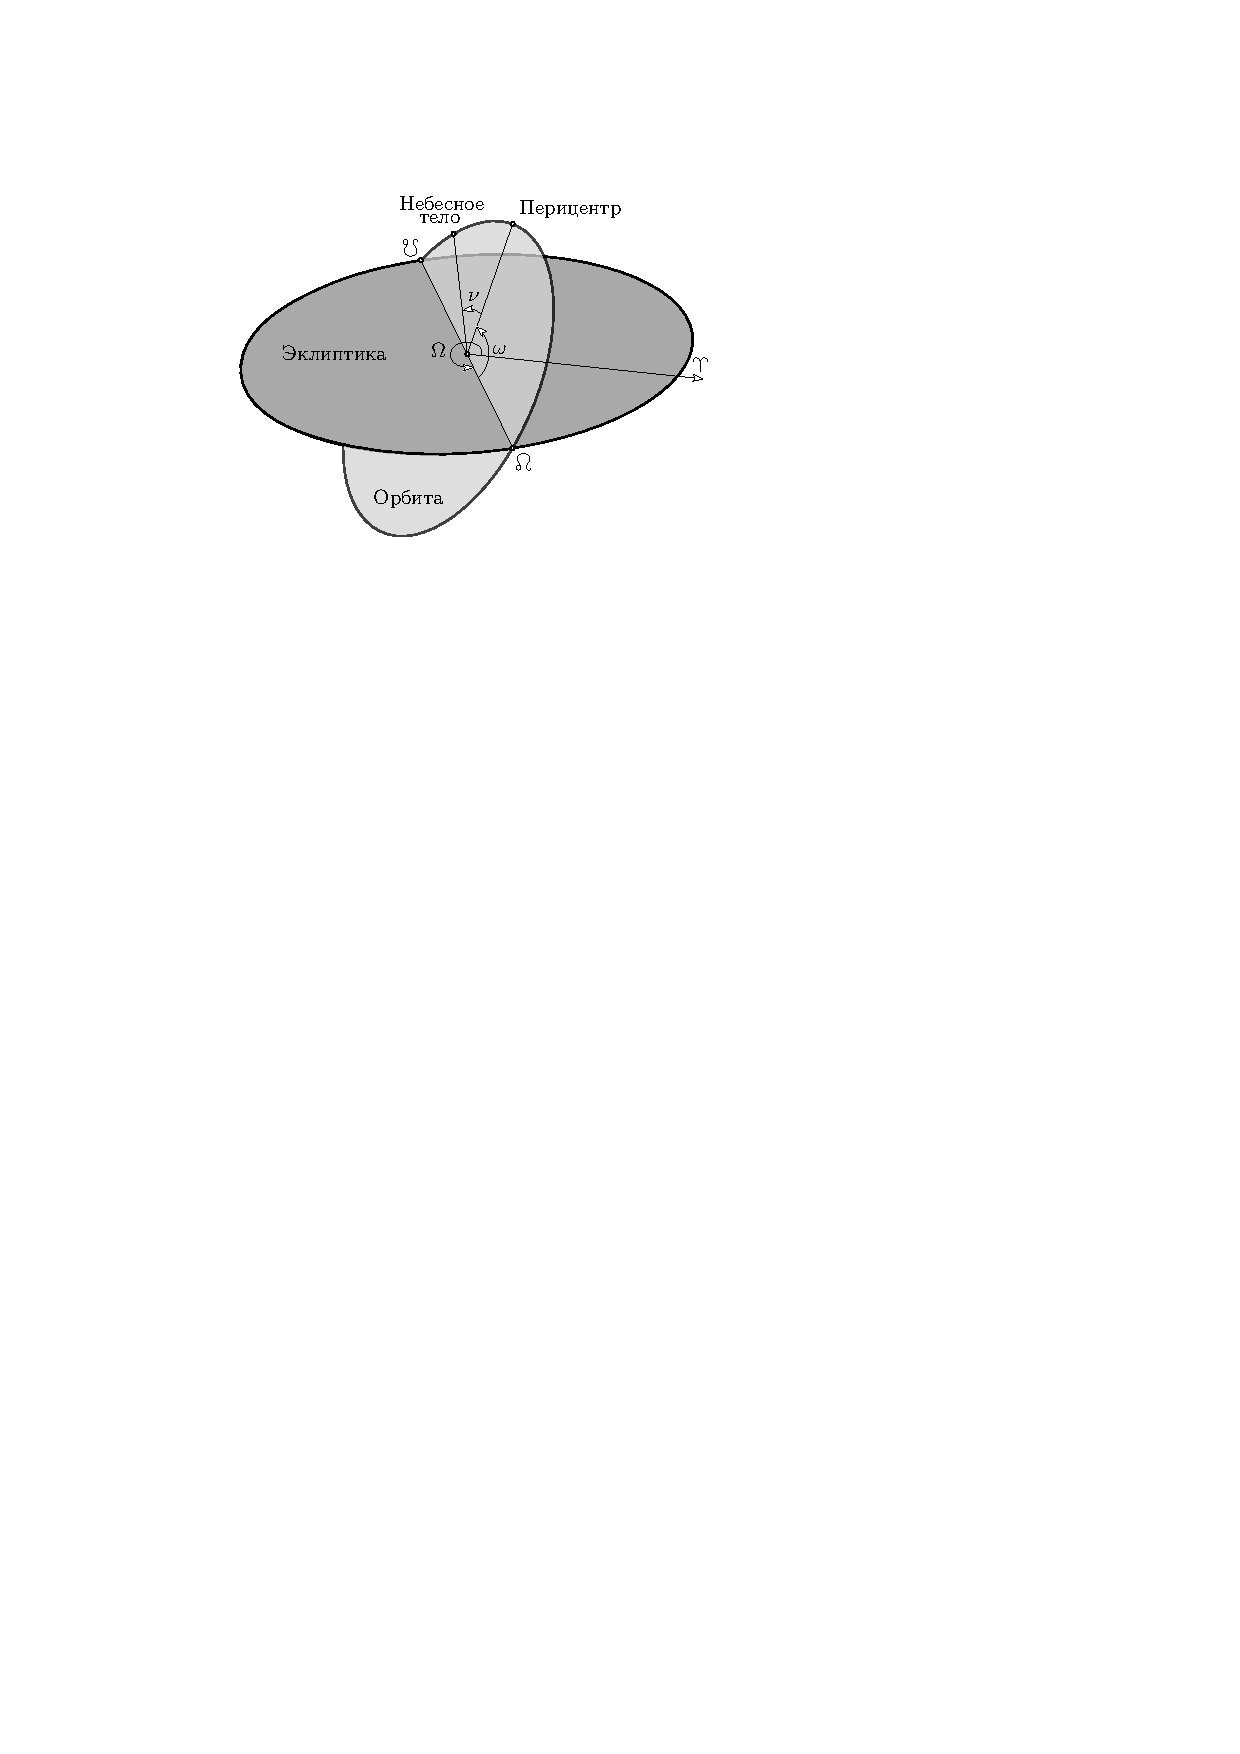
\includegraphics[width=.45\tw]{orbit-elem}
	\captionof{figure}{Кеплеровы элементы орбиты}
	\label{fig:orb-elem}
\end{wrapfigure}
небесного тела в пространстве в задаче двух тел: \imp{большая полуось} ($a$), \imp{эксцентриситет} ($e$), \imp{наклонение} ($i$), \imp{аргумент перицентра} ($\omega$), \imp{долгота восходящего узла} ($\Omega$), \imp{средняя аномалия} ($M_0$). Первые два определяют форму орбиты, третий, четвёртый и пятый~--- ориентацию плоскости орбиты по отношению к базовой системе координат, связанной с эклиптикой, последний~--- положение тела на орбите~(см.~Рис.\,\ref{fig:orb-elem}).

\term{Наклонение}~--- это угол между плоскостью орбиты небесного тела и плоскостью эклиптики.

\term{Аргумент перицентра}~--- угол между направлениями на восходящий узел орбиты и на перицентр при наблюдении из притягивающего центра.

\term{Долгота восходящего узла}~--- угол в плоскости эклиптики между направлением на точку весеннего равноденствия и восходящий узел орбиты. Отсчитывается против часовой стрелки от направления на точку весеннего равноденствия.

\term{Средняя аномалия} для тела, движущегося по невозмущённой орбите~--- произведение его среднего движения и интервала времени после прохождения перицентра.

\term{Узлы орбиты}~--- точки пересечения орбиты и плоскости эклиптики. \imp{Восходящий узел}~--- точка, в которой тело пересекает плоскость эклиптики при движении в северноим направлении, а \imp{нисходящий}~--- в южном.

\term{Истинная аномалия}~($\nu$)~--- угол между радиус-вектором и направлением на перицентр.
\subsection{Точки Лагранжа}

\term{Точки Лагранжа}~--- точки, во вращающейся системе из двух массивных тел,
\begin{wrapfigure}[14]{l}{0.48\tw}
	\centering
	\vspace{-.5pc}
	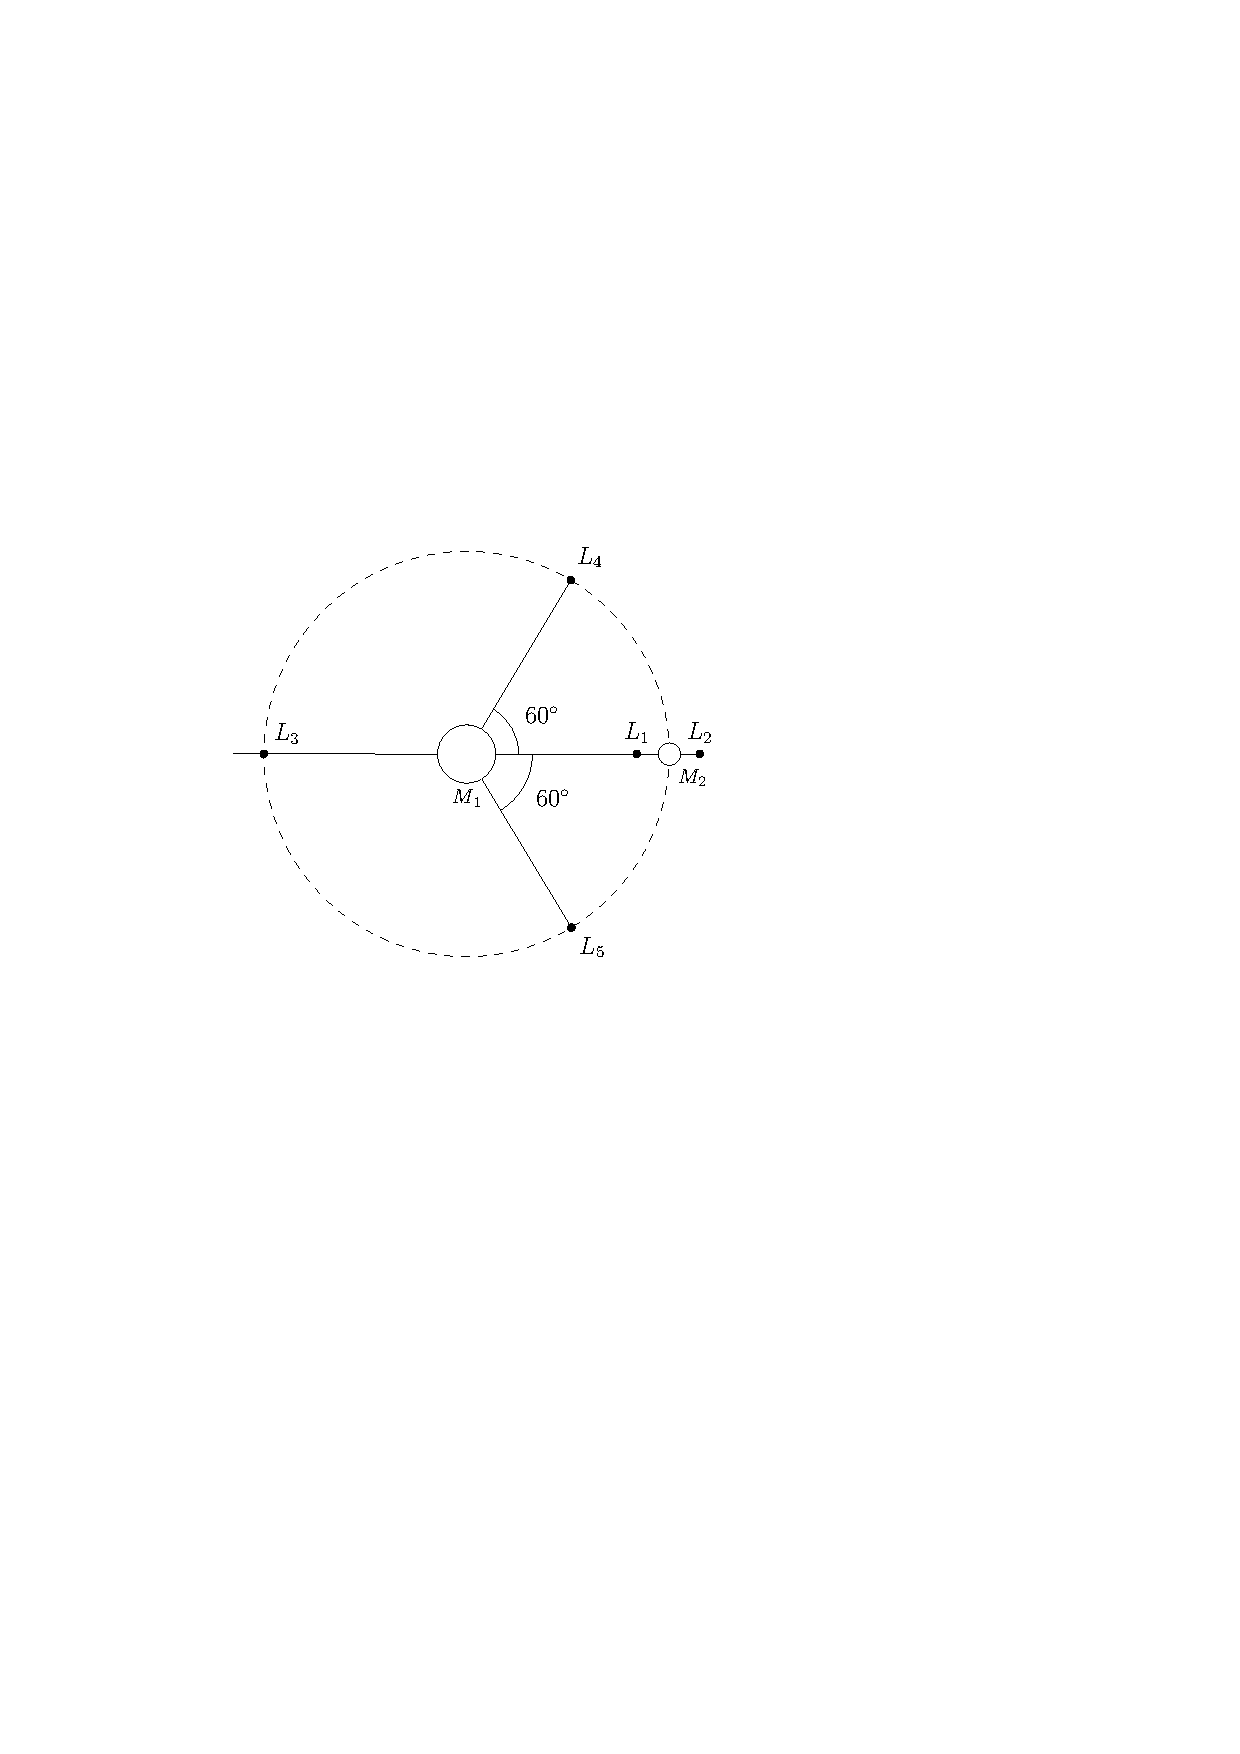
\includegraphics[width = .48\tw]{lagr-points}
	\captionof{figure}{Точки Лагранжа}
	\label{pic:larg-points}	
\end{wrapfigure}
в которых третье тело с пренебрежимо 
малой массой, не испытывающее воздействие никаких 
других сил, кроме гравитационных, со стороны двух 
первых тел, может оставаться неподвижным относительно 
этих тел. В этих точках гравитационные силы, 
действующие на малое тело, уравновешиваются силами инерции.

Точки $L_1$, $L_2$ и $L_3$ лежат на одной прямой, 
соединяющей два массивных тела. Точки $L_4$ и $L_5$ 
образуют равносторнние треугольники с массивными 
телами.

Для расстояний до точек $L_1$, $L_2$ и $L_3$ от 
центра масс системы справедливы следующие выражения:
\begin{equation}r_1=R\left(1-\sqrt[3]{\frac{\alpha}
{3}}\right), \quad r_2=R\left(1+\sqrt[3]{\frac{\alpha}
{3}}\right), \quad r_3=R\left(1+\frac{5}{12}\alpha\right),
\end{equation}
где $\alpha=M_2 / (M_1 + M_2)$, $R$~--- расстояние между 
телами, $M_1$ --- масса более массивного тела, $M_2$
 --- масса второго тела.

Если $M_2 \ll M_1$, то точки $L_1$ и $L_2$ находятся 
примерно на одинаковом расстоянии от тела $M_2$, равном
\begin{equation}
r\approx R\sqrt[3]{\frac{M_2}{3M_1}}.
\end{equation}

Расстояния от центра масс системы до точек $L_4$ и $L_5$ в координатной системе с центром координат в центре масс системы рассчитываются по  формулам
\begin{equation}
	 r_4 = \left ( \frac{R}{2} \cdot \frac{M_1-M_2}{M_1+M_2} ,   \frac{\sqrt{3}R}{2} \right ), \quad r_5 = \left ( \frac{R}{2} \cdot \frac{M_1-M_2}{M_1+M_2} ,   -\frac{\sqrt{3}R}{2} \right ). 
\end{equation}
\subsection{Приливы и отливы}

\term{Приливы и отливы}~--- периодические вертикальные колебания уровня океана, являющиеся результатом изменения положения Луны и Солнца. Хотя силы тяготения Солнца почти в 200 раз больше, чем силы тяготения Луны, приливные силы, порождаемые Луной, почти вдвое больше порождаемых Солнцем. Это происходит из-за того, что приливные силы зависят не от величины гравитационного поля, а от степени его неоднородности. Высота приливов зависит от взаимного расположения Луны и Солнца: наибольший~---  силы от Луны и от Солнца действуют вдоль одного направления, а наименьший~--- под прямым углом друг к другу.

\begin{minipage}{.24\tw}
Ускорение в центре Земли ($T$) определяется формулой \eqref{eq:g}:
\begin{equation*}
	a_T=\frac{G M}{r^2},
\end{equation*}
$M$~--- масса возмущающего тела,
\end{minipage}
\hfill
\begin{minipage}{0.74\tw}
	\vspace{-.5pc}
	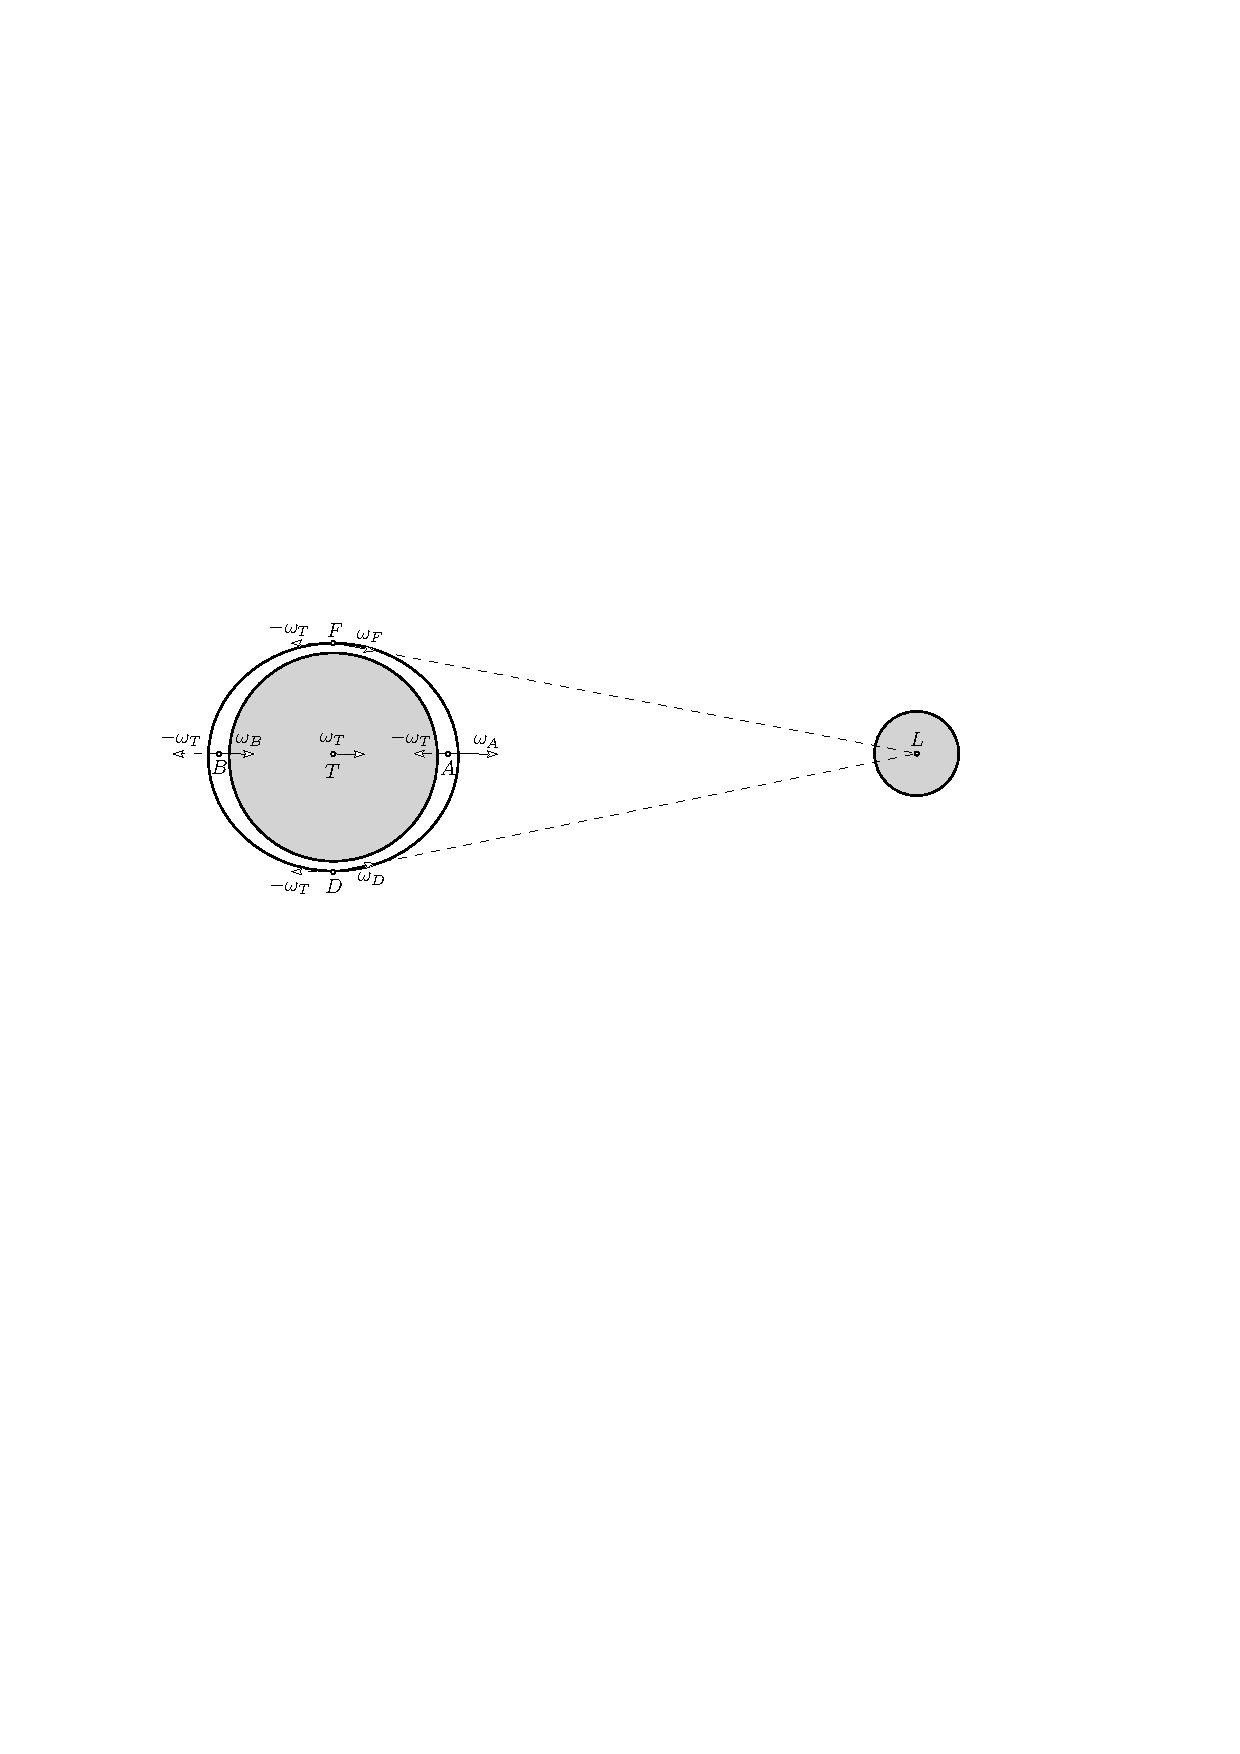
\includegraphics[width = \tw]{Ebb_flow}
	\captionof{figure}{К объяснению приливных сил}\label{Ebb_flow}
\end{minipage}\\[-0.5pc]

$r$~--- расстояние между центрами Земли и данного тела. Аналогично, ускорения в точках $A$ и $B$ равны соответственно
\begin{equation}
	a_A = \frac{G M}{(r - R)^2} \quad \text{и} \quad a_B = \frac{GM}{(r + R)^2},
\end{equation}
где $R$~--- радиус Земли или иного тела, подверженного воздействию приливных сил. Ускорение в точке $A$ относительно точки $T$ равно
\begin{equation}
	a_A - a_T = a_T \cdot \frac{2 r R - R^2}{(r - R)^2} = \frac{GM \left(2 r R - R^2 \right)}{r^2 (r - R)^2} \xrightarrow{R \ll r} \frac{2 G M R}{r^3}.
	\label{eq:ebb-force}
\end{equation}

Под действием лунного притяжения водная оболочка Земли принимает форму 
эллипсоида, который вытянут по направлению к Луне. Близ точек $A$ и $B$ будет 
прилив, а в точках $F$ и $D$ --- отлив (см.~Рис.\,\ref{Ebb_flow}).
\nopagebreak
\subsection{Затмения}
Диаметр тени спутника при полном центральном затмении (когда центры трёх тел лежат на одной прямой), с большой точностью равен: 
\begin{equation}
d_\text{тени} = 2 \cdot \frac{R_{\moon}(a_\oplus - R_\oplus) - R_\odot \left( a_{\moon} - R_\oplus \right)}{a_\oplus - a_{\moon}}.
\end{equation}
Среднее значение  этой величины около 200 км, максимальное около 215 км. При нецентральном затмении максимальный диаметр тени Луны на поверхности Земли может достигать 270~км. Что дает оценку на продолжительность~--- 7.5~минут. Большинство же полных затмений длятся 2\,--\,4~минуты.

\begin{figure}[h!]
\centering
\vspace{-.5pc}
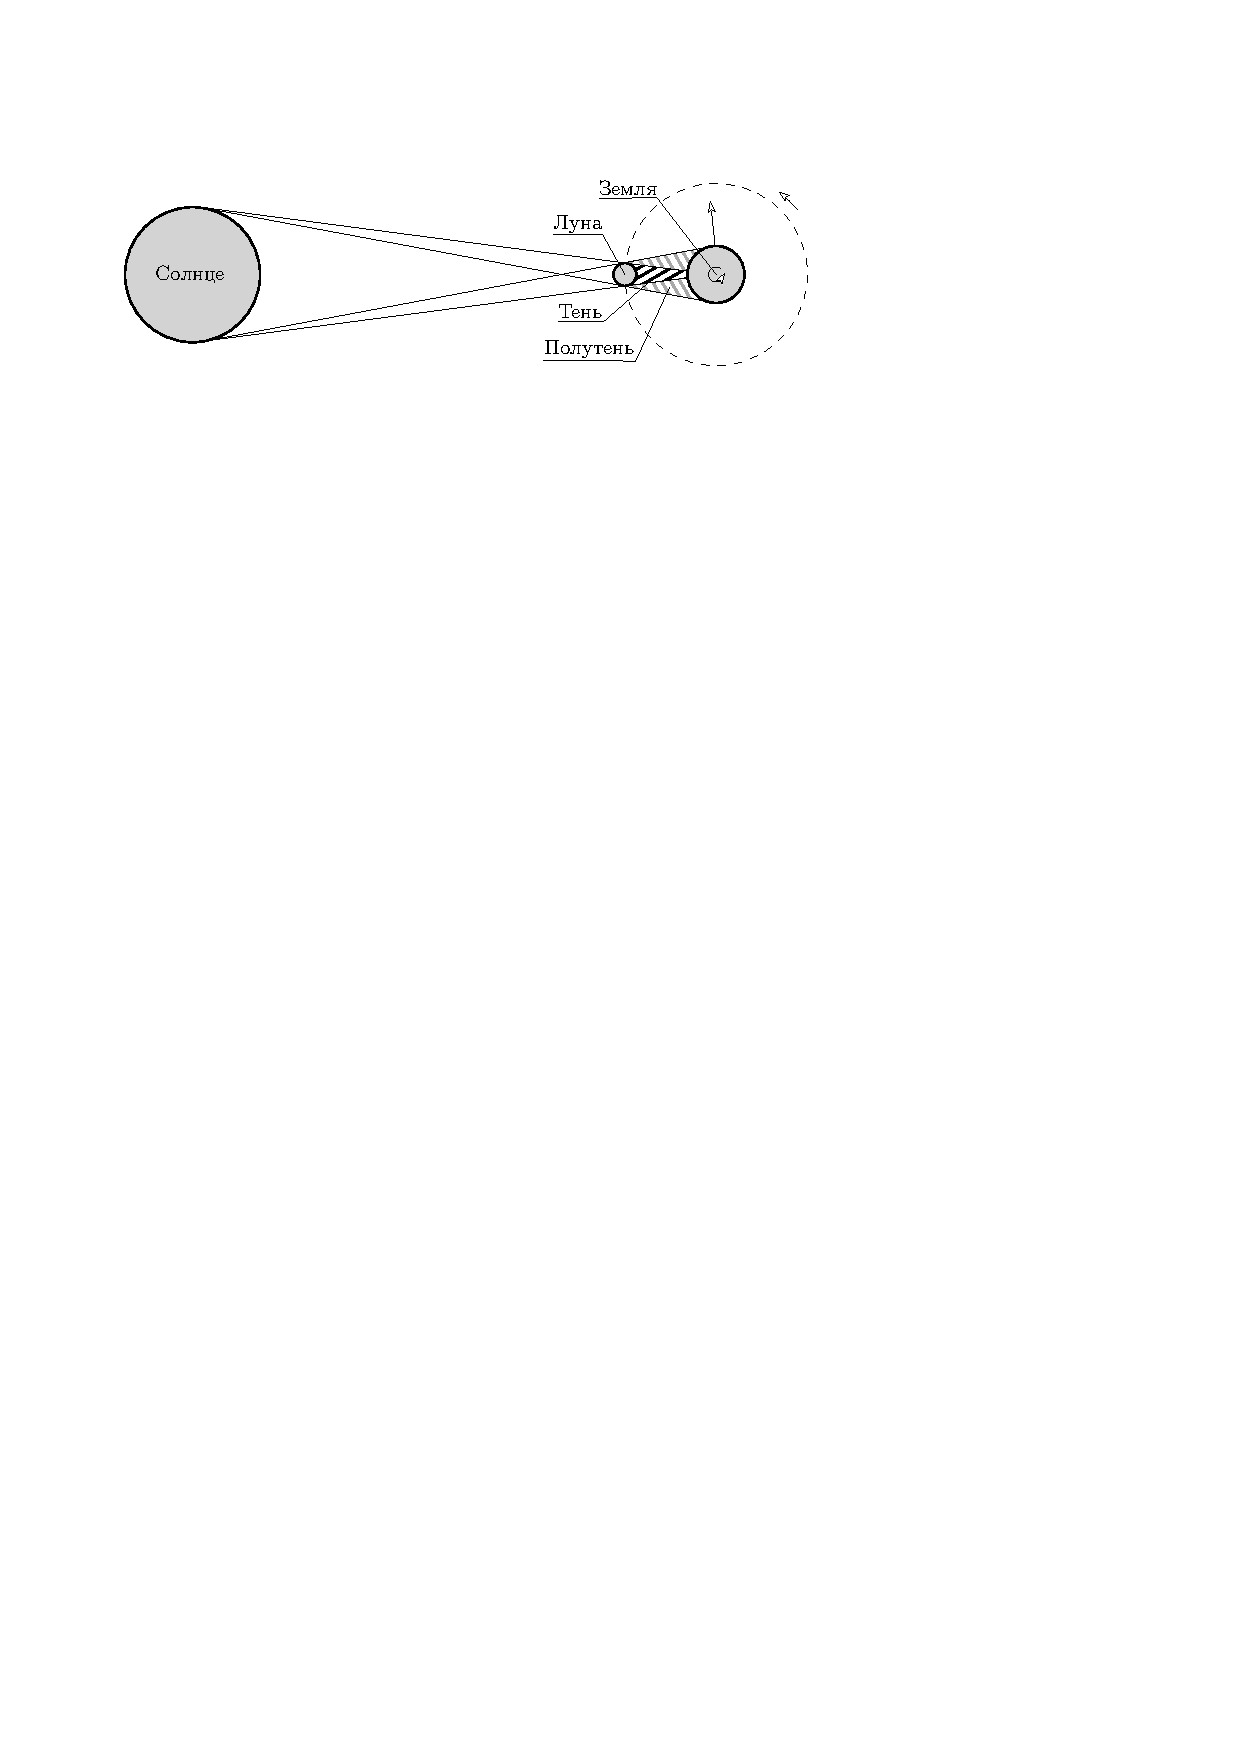
\includegraphics[width = 10cm]{full_eclipse}
\caption{Полное солнечное затмение со стороны северного полюса эклиптики}
\label{fig:eclipses-full-solar-eslipse}
\end{figure}
При \term{кольцеобразном солнечном затмении} Луна относительно Земли расположена так, что конус её тени не достаёт до поверхности планеты, и вокруг Луны можно наблюдать яркое кольцо незакрытой части солнечного диска.

\begin{figure}[h!]
	\centering
	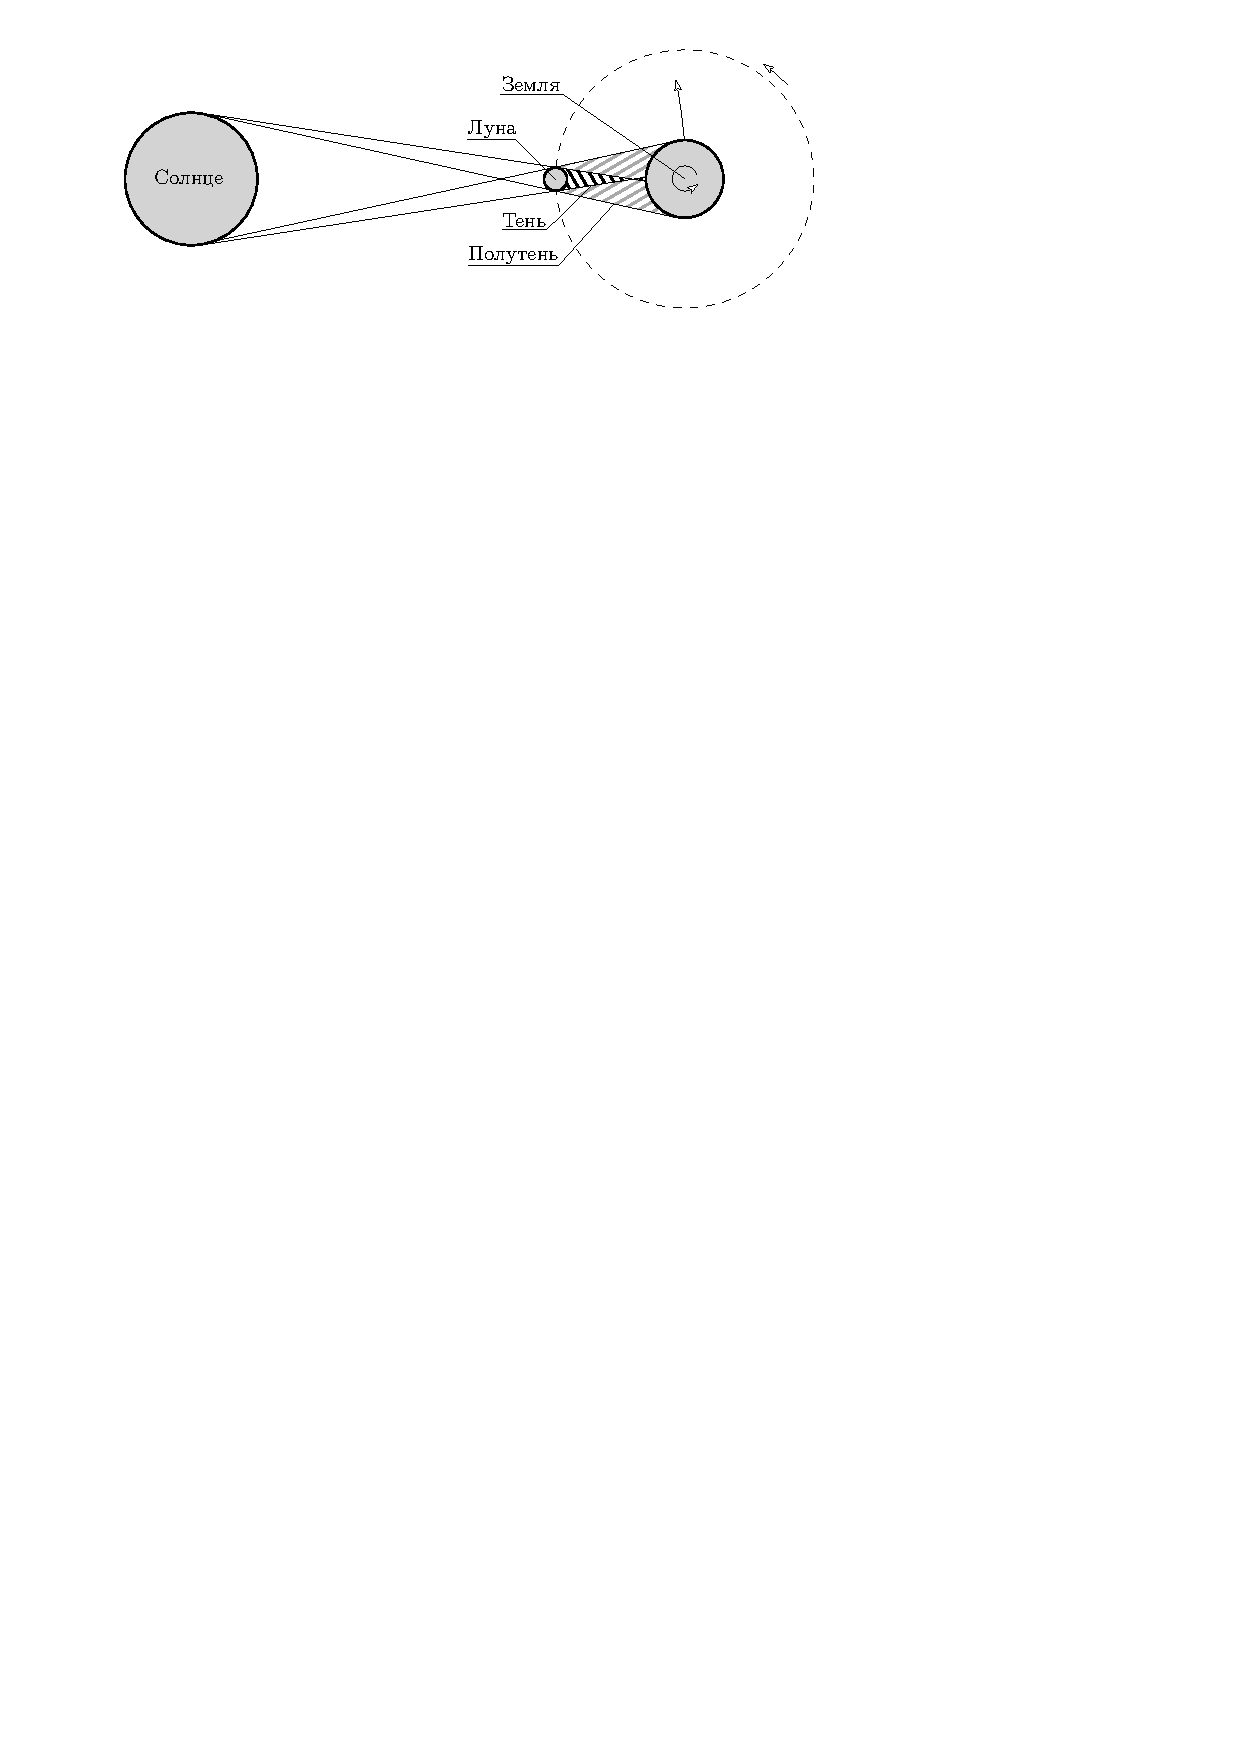
\includegraphics[width = 10cm]{partly-eclipse}
	\caption{Кольцеобразное солнечное затмение со стороны северного полюса эклиптики}
	\label{fig:eclipses-circle-solar-eslipse}
\end{figure}
При особом расположении Луны и Земли возможны \term{гибридные} затмения, когда в разных пунктах Земли наблюдаются \imp{кольцеобразное} и \imp{полное} затмение. Причиной такого явления является шарообразность Земли.

\vspace{-1pc}
\begin{figure}[h!]
	\centering
	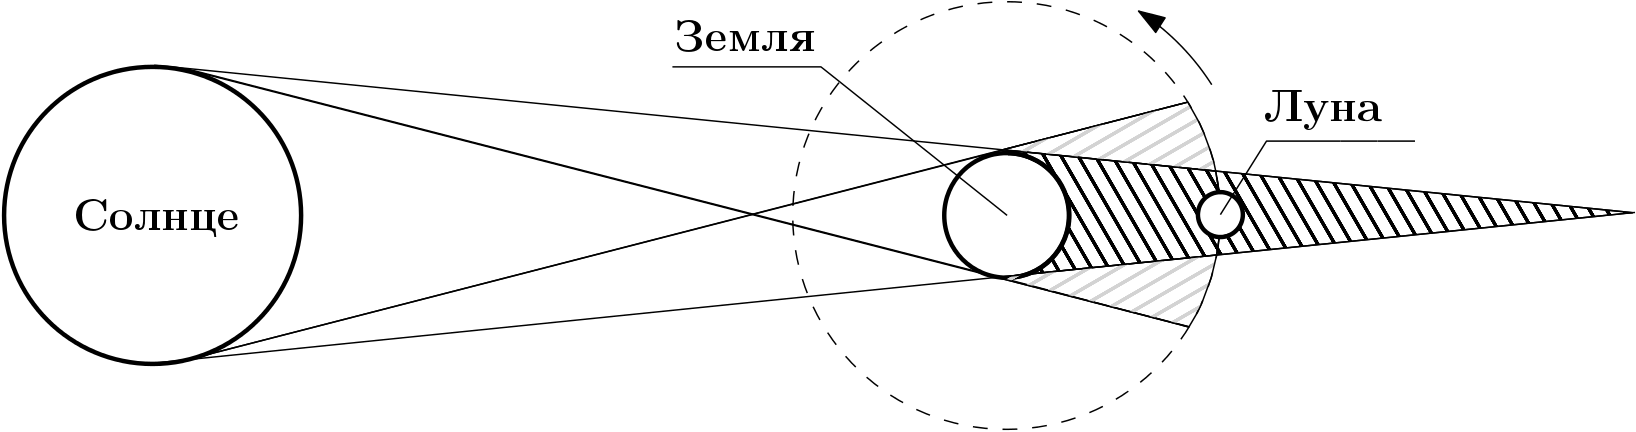
\includegraphics[width=10cm]{moon-eclipse}
	\caption{Схема лунного затмения со стороны северного полюса эклиптики}
	\label{fig:moon-eclipse-scheme}
\end{figure}
\term{Лунное затмение} в отличие от солнечного, видно со всего ночного полушария Земли. Диаметр земной тени на расстоянии Луны превышает размер последней примерно в 2.5\,--\,3 раза. Бывают \term{частные}, когда лишь части Луны попадает в земную тень, \term{полные}~--- Луна полностью погружается в тень Земли, и \term{полутеневые}~--- Луна проходит через полутень Земли, не затрагивая конус тени.

\term{Синодический месяц}~--- промежуток времени между одинаковыми фазами Луны, равен 29.53 суток.

\term{Драконический месяц}~--- промежуток времени между двумя последовательными прохождениями Луны через один и тот же узел орбиты,~--- 27.21 суток.

\term{Сарос}~--- промежуток  времени, по прошествии которого солнечные и лунные затмения повторяются в прежнем порядке. Происходит это из-за того, что каждый сарос Луна, орбита Луны и Солнце возвращаются в прежнее положение относительно далёких звёзд. Сарос длится ровно 242 драконических месяца, или 223 синодических месяца, или 18 лет 11 дней 8 часов.

\begin{wrapfigure}[8]{r}{.42\tw}
	\centering
	\vspace{-1pc}
	\includegraphics[width = 0.2\textwidth]{phases}
	\hfill
	\includegraphics[width = 0.2\textwidth]{phases-2}
	\caption{Частное и полное затмение}
	\label{fig:part-eclipses-scheme}
\end{wrapfigure}
Важной характеристикой любого затмения является его \term{фаза}~--- для \imp{частных} и \imp{кольцеобразных} затмений: отношение закрытой части $x$ диаметра\footnote{Здесь имеется в виду \imp{угловой} диаметр} затмеваемого тела, проходящего через центр затмевающего тела, ко всему диаметру затмеваемого тела $D$; для \imp{полного}: единица плюс отношение расстояния\footnote{Расстояние между окружностями $l_1$ и $l_2$~--- это $\min |L_1L_2|$ по всем $L_1 \in l_1$ и $L_2 \in l_2$.} между краями дисков затмеваемого и затмевающего тел к диаметру затмеваемого тела $D$.
\begin{equation}
\Phi_{\text{част}} = \frac{x}{D} < 1, \quad \quad \quad \Phi_{\text{полн}} =  1 + \frac{\min\{d_1, d_2\}}{D} > 1.
\end{equation}
Иногда вводят такое понятие, как \term{площадная фаза затмения}, т.\,е. отношение площади закрытой части диска затмеваемого диска к полной площади его диска. Чаще всего  площадную фазу используют применительно к двойным звёздам, когда считают падение блеска при затмении одной звезды другой.

\subsection{Конфигурации планет}
\term{Внутренними планетами} называются планеты, большая полуось орбиты 
$a$ которых меньше большой полуоси орбиты Земли $a_\oplus$. Отсюда следует, что для наблюдателя на Земле \imp{внутренними} планетами являются лишь Венера и Меркурий, остальные относятся к \imp{внешним}. Для таких планет выделяют три основные конфигурации: \imp{верхнее соединение}, \imp{нижнее соединение} и \imp{максимальная элонгация}. Различают две максимальные элонгации~--- \term{западную} и \term{восточную}, когда планета наблюдается к западу и к востоку от Солнца соответственно.

Внутренняя планета находится в \term{верхнем соединении}, когда Земля, Солнце и планета лежат на одной прямой, при этом планета и Земля располагаются по разные стороны от Солнца. Если пренебречь наклоном орбит планет к плоскости эклиптики, то для наблюдателя на Земле планета находится точно за Солнцем.

\begin{minipage}{0.36\tw}
\term{Нижнее соединение} внутренней планеты происходит когда Земля, Солнце и планета, также как и в случае верхнего соединения, располагаются на одной прямой, но для нижнего соединения планета должна находиться между Солнцем и Землей. Если бы орбиты всех планет лежали в одной плоскости, тогда в момент каждого нижнего соединения внутренней планеты наблюдалось бы ее прохождение по диску Солнца для наблюдателя на внешней планете.
\end{minipage}
\begin{minipage}{0.63\tw}
	\centering
	\vspace{-1pc}
	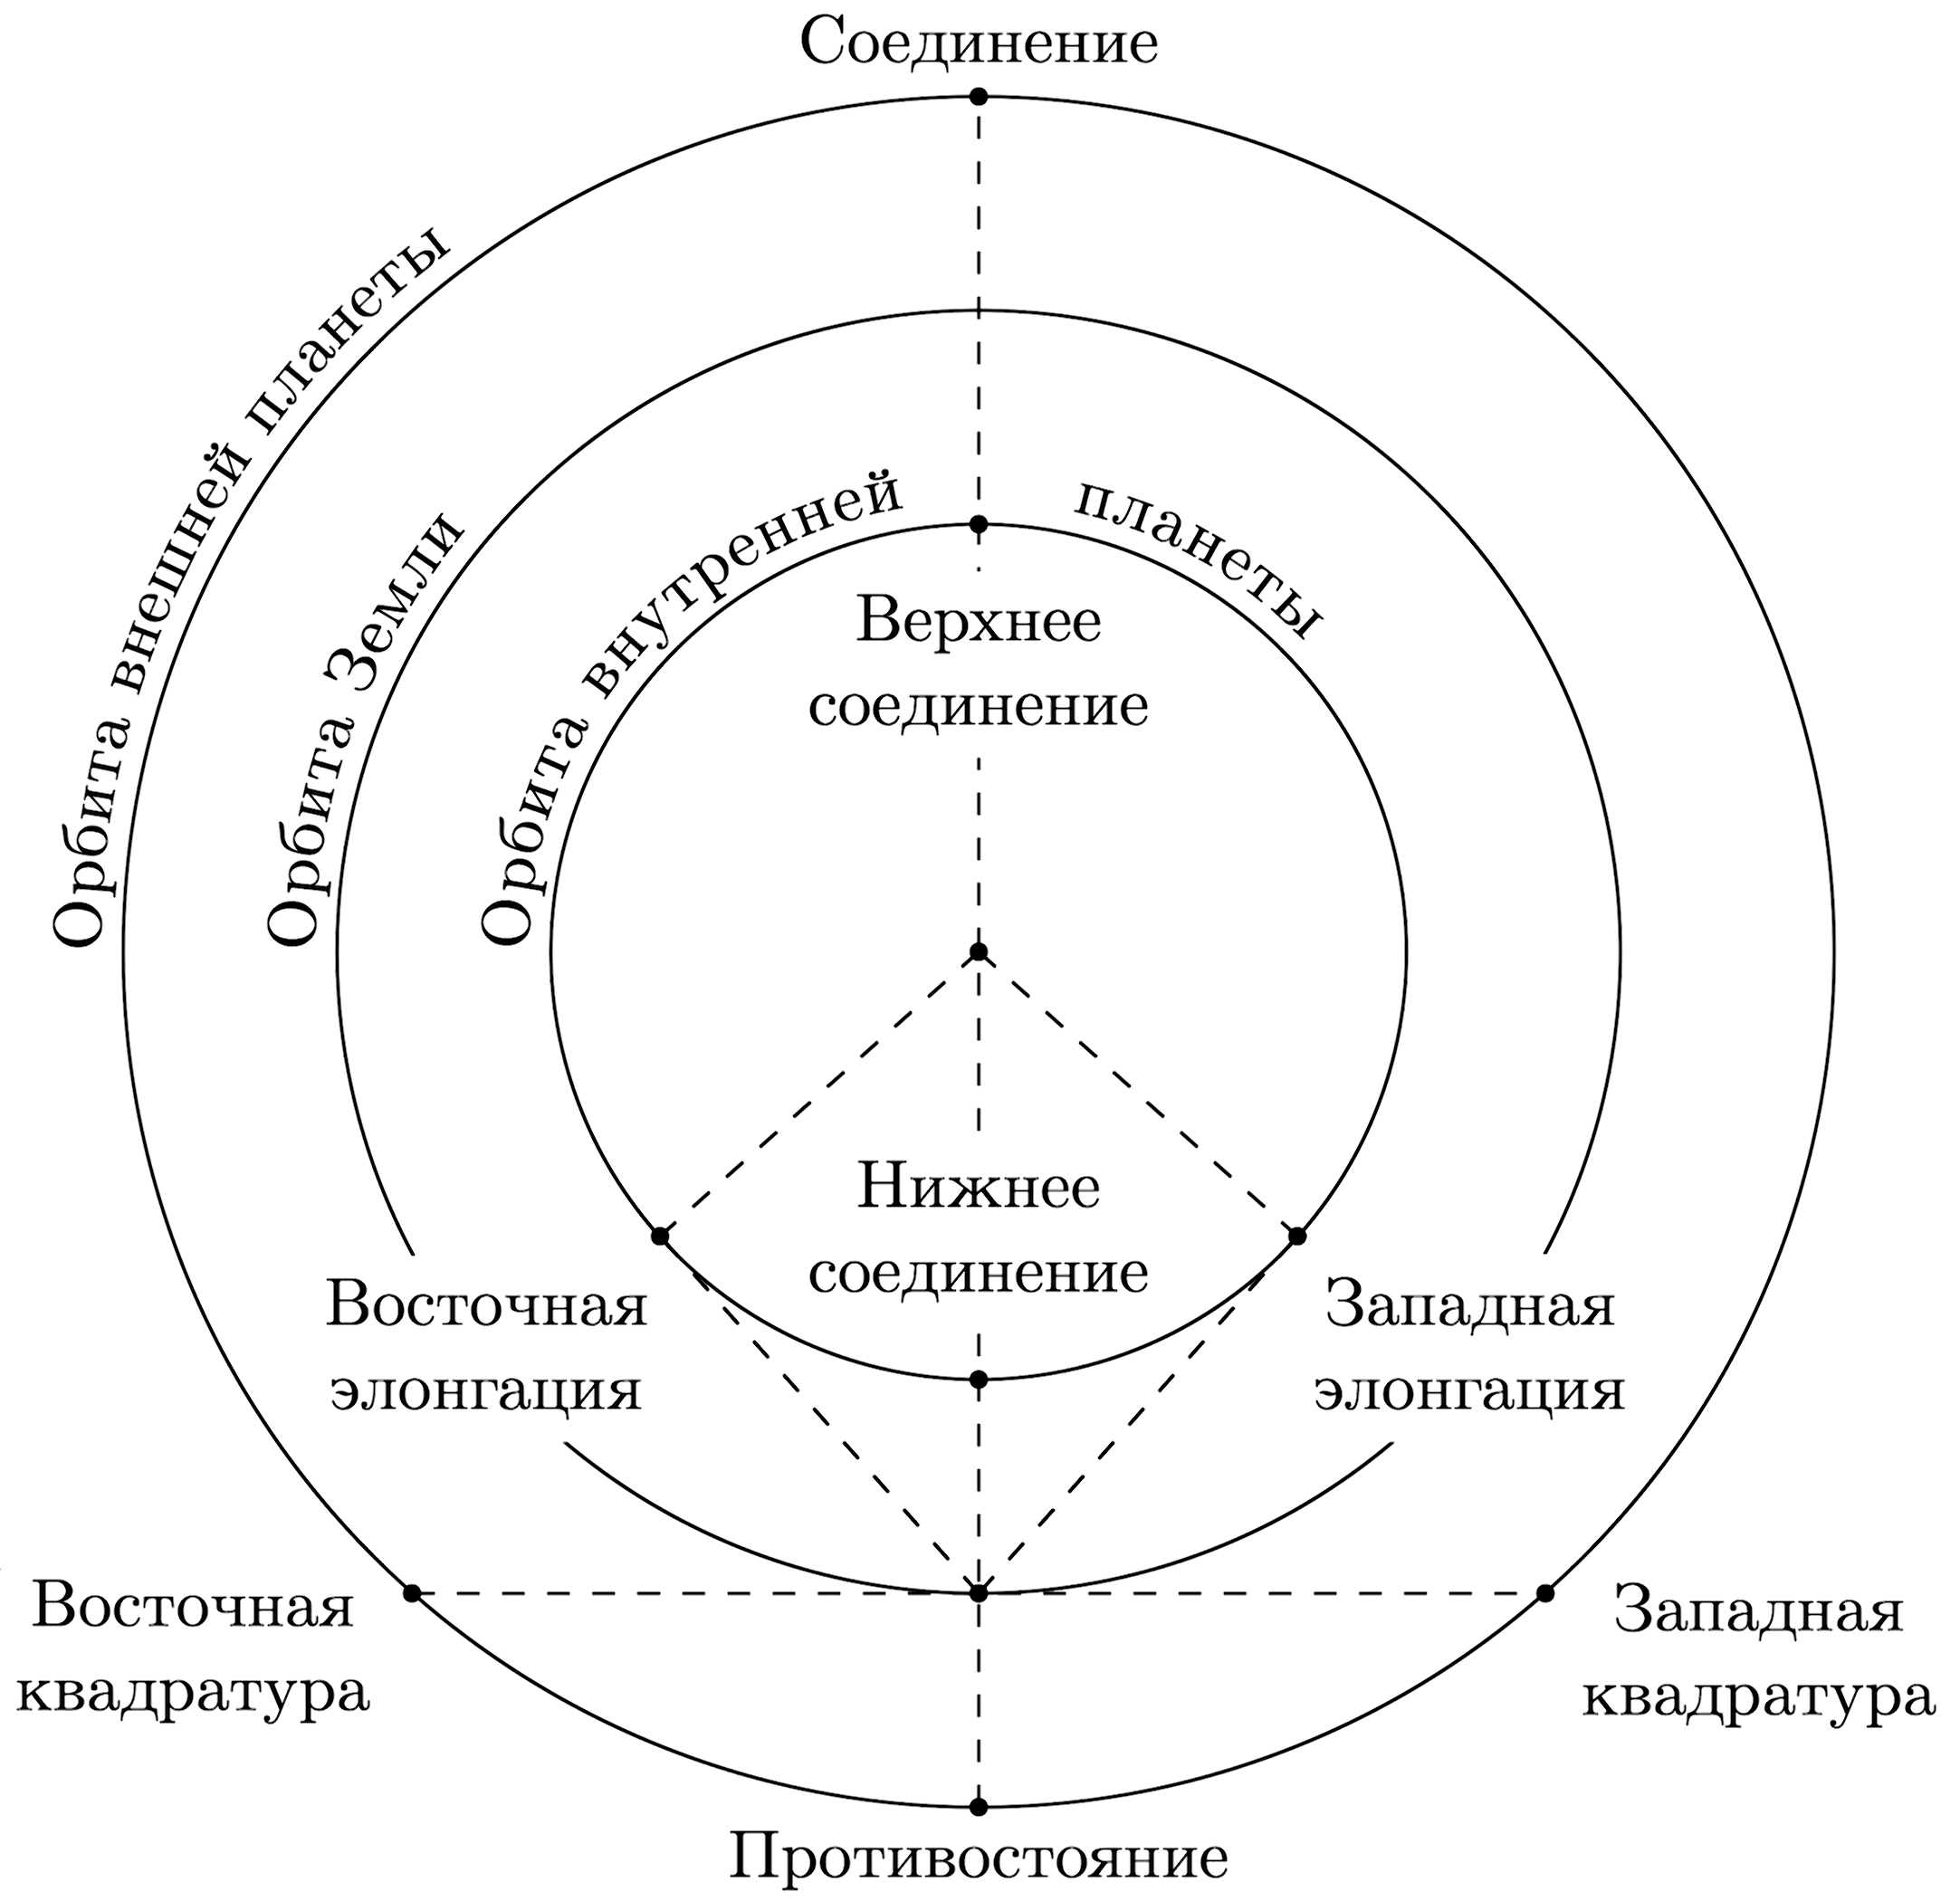
\includegraphics[width=\tw]{planet-config}
%\scriptsize
%\begin{tikzpicture}
%\fill [draw=black, fill=none,
%         postaction={decorate,decoration={raise=3pt,text along path, 
%           text={Орбита Земли}}}
%]
%  (-2.5, 0) arc (180:-180:2.5cm and 2.5cm);
%
%\fill [draw=black, fill=none,
%         postaction={decorate,decoration={raise=3pt,text along path,
%           text={Орбита внутренней~~~~~~~планеты}}}
%           ]
%  (-1.5, 0) arc (180:-180:1.5cm and 1.5cm);
%
%\fill [draw=black, fill=none,
%         postaction={decorate,decoration={raise=3pt,text along path,
%           text={Орбита внешней планеты}}}
%           ]
%  (-3.5, 0) arc (180:-180:3.5cm and 3.5cm);
%  
%\draw [dashed] (-2.65, -3) -- (2.65, -3);
%\draw [dashed] (0, -4) -- (0, 4);
%\draw [dashed] (0, -3) -- (-1.49, -1.33);
%\draw [dashed] (0, 0) -- (-1.49, -1.33);
%\draw [dashed] (0, -3) -- (1.49, -1.33);
%\draw [dashed] (0, 0) -- (1.49, -1.33);
%
%\filldraw [black] (0, 0) circle (1pt);
%\filldraw [black] (-1.49, -1.33) circle (1pt);
%\filldraw [black] (1.49, -1.33) circle (1pt);
%\filldraw [black] (2.65, -3) circle (1pt);
%\filldraw [black] (-2.65, -3) circle (1pt);
%\filldraw [black] (0, -3) circle (1pt);
%\filldraw [black] (0, 2) circle (1pt);
%\filldraw [black] (0, 4) circle (1pt);
%\filldraw [black] (0, -2) circle (1pt);
%\filldraw [black] (0, -4) circle (1pt);
%
%\draw (-3.7, -3.7) -- (-3.7, -3.7) node  [above,align=center,midway]{Западная\\квадратура};
%    
%\draw (3.7, -3.7) -- (3.7, -3.7) node  [above,align=center,midway]{Восточная\\квадратура};
%    
%\draw (0, -4.5) -- (0, -4.5) node  [above,align=center,midway]{Противостояние};
%
%\draw (0, 4) -- (0, 4) node  [above,align=center,midway]{Соединение};
%
%\draw (0, 0.9) -- (0, 0.9) node  [fill=white,above,align=center,midway]{Верхнее\\соединение};
%
%\draw (0, -1.75) -- (0, -1.75) node  [fill=white,above,align=center,midway]{Нижнее\\соединение};
%
%\draw (0.6, -3.4) -- (0.6, -3.4) node  [above,align=center,midway]{\ttfamily Земля};
%
%\draw (0.7, -0.2) -- (0.7, -0.2) node  [above,align=center,midway]{\ttfamily Солнце};
%
%\draw (2.3, -2.3) -- (2.3, -2.3) node  [fill=white,above,align=center,midway]{Западная\\элонгация};
%
%\draw (-2.3, -2.3) -- (-2.3, -2.3) node  [fill=white,above,align=center,midway]{Восточная\\элонгация};
%
%\end{tikzpicture}
	\captionof{figure}{Конфигурации планет}
\end{minipage}\\

\term{Элонгацией} планеты называется угол Солнце -- Земля -- планета, отсюда очевидно, что \imp{максимальная элонгация} внутренней планеты наблюдается в момент, когда прямая Земля -- планета является касательной к орбите планеты, то есть угол Солнце -- планета -- Земля является прямым.

\term{Внешними планетами} называются планеты, большая полуось орбиты $a$ которых больше большой полуоси орбиты Земли $a_\oplus$. Для таких планет также существуют три основные конфигурации: \imp{соединение}, \imp{противостояние} и \imp{квадратура}. Квадратура бывает \term{западная} и \term{восточная}, в какой именно квадратуре находится внешняя планета определяется аналогично максимальной элонгации.

\term{Соединение} внешней планеты, подобно верхнему соединению внутренней планеты, наблюдается в момент, когда Солнце, Земля и планета находятся на одной прямой, при этом Солнце находится между планетой и Землей. В этот момент для наблюдателя на внешней планете Земля, являясь нижней планетой, наблюдается в верхнем соединении.

Аналогично, когда планета, Солнце и Земля располагаются на одной прямой, но Солнце и планета лежат по разные стороны от Земли, считается, что внешняя планета находится в \term{противостоянии}. Земля же находится в нижнем соединении для наблюдателя на внешней планете, наблюдаемой в противостоянии.

\term{Квадратурой} называется конфигурация, когда угол между направлениями на планету и Солнце (угол {\slshape Солнце -- Земля -- планета}) является прямым. Стоит заметить, что для наблюдателя на планете Земля будет наблюдаться в максимальной элонгации, причем если планета с Земли наблюдалась в восточной квадратуре, тогда Земля будет в западной максимальной элонгации и наоборот.


\subsection{Фазы планет и спутников}

\term{Фаза} планеты (спутника)~--- отношение площади освещённой  части видимого диска ко всей его площади.
Фаза рассчитывается по формуле
\begin{equation}
\Phi = \frac{1 + \cos \phi}{2} = \cos^2 \frac{\phi}{2},
\end{equation}
\begin{minipage}{0.67\tw}
где $\phi$~--- \term{фазовый угол} --- угол между лучом света, падающим от Солнца на планету, и лучом, отразившимся от неё в сторону наблюдателя (см.~Рис.\,\ref{fig:phase-angel-scheme}). Фаза объекта может принимать значения от 0 до 1.

Видимая граница между освещенной и неосвещенной частями поверхности объекта называется \term{терминатором}. В зоне терминатора для наблюдателя на объекте источник пересекает горизонт.
\end{minipage}
\hfill
\begin{minipage}{0.31\tw}
	\hfill
	\vspace{-.5pc}
	\includegraphics[width = \tw]{phase-angle}
	\captionof{figure}{Фазовый угол}
	\label{fig:phase-angel-scheme}
\end{minipage}


\subsection{Синодический период}

\term{Синодический период} (период смены фаз)~--- время, прошедшее между двумя последовательными одноимёнными конфигурациями одного тела при наблюдении с другого.

\imp{Относительная угловая скорость} планет равна 
разности скоростей углового перемещения одной планеты ($2\pi/T_1$) и другой ($2\pi/T_2 $) по орбите. Из определения относительной угловой скорости вытекает общая формула для продолжительности синодического периода: 
\begin{equation}
\frac1S=\left| \frac{1}{T_1}-\frac{1}{T_2} \right|.
\end{equation}
Для внешних и внутренних планет соответственно выражения принимают следующий вид: 
\begin{equation} \frac{1}{S} = \frac{1}{T_\oplus} - \frac{1}{T_\text{пл}} \quad \text{и} \quad \frac{1}{S} = \frac{1}{T_\text{пл}} - \frac{1}{T_\oplus},
\end{equation}
где $S$~--- синодический период, $T_\text{пл}$~--- сидерический период планеты, $T_\oplus$~--- сидерический период обращения Земли.

В случае, если тела обращаются в противоположные стороны, то связь 
их синодического периода с сидерическими очевидным образом принимает вид:
\begin{equation}
\frac{1}{S} = \frac{1}{T_1} + \frac{1}{T_2}.
\end{equation}
\subsection{Собственное движение звёзд}
\term{Собственным движением} $(\mu)$ называется изменение координат звёзд на небесной сфере, вызванное относительным движением звёзд и Солнца, обычно измеряется в mas/год.
\begin{equation}
	\mu = \frac{V_\tau}{D},
\end{equation}
где $V_\tau$~--- тангенциальная относительная скорость звезды, $D$~--- расстояние до неё.

\change{Разделяют также собственное движение по склонению~--- $\mu_\delta$ и собственное движение по прямому восхождению~--- $\mu_\alpha$, которые определяются следующими выражениями:}
\begin{equation}
	\mu_\delta = \frac{\delta(t_2) - \delta(t_1)}{t_2 - t_1}, \quad \quad \mu_\alpha = \frac{\alpha(t_2) - \alpha(t_1)}{t_2 - t_1}.
\end{equation}
\change{
\begin{wrapfigure}{r}{.4\tw}
	\begin{flushright}
		\vspace{-1pc}
		\begin{tikzpicture}
			\footnotesize
			\draw [dashes] (0, 4) arc(90:0:3 and 4);
			\draw [dashes] (0, 4) arc(90:0:2 and 4);
			%
			\draw [dashes] (3.47, 2) arc(0:-70:3.47 and 1.16);
			\draw [dashes] (2.64, 3) arc(0:-70:2.64 and 0.88);
			%
			\draw [thick, -latex] (2.3, 2.55) arc(-34:-56:2.64 and 0.88);
			\draw [thick, -latex] (2.3, 2.55) arc(53:29:2 and 4);
			\draw [thick, -latex] (2.3, 2.55) .. controls (2.3, 1.9) and (2.1, 1.4) .. (1.93, 1.03);
			%
			\draw (.9, 2.2) node [anchor=south] {$\delta(t_1)$};
			\draw (1.2, .9) node [anchor=south] {$\delta(t_2)$};
			%
			\draw (2, 0) node [anchor=north] {$\alpha(t_2)$};
			\draw (3, 0) node [anchor=north] {$\alpha(t_1)$};
			%
			\draw [fill=white] (2.3, 2.55) circle (0.03);
			\draw [fill=white] (1.93, 1.03) circle (0.03);
			\draw [fill=white] (0, 4) circle (0.03);
			%
			\draw (0, 4) node [anchor=north] {$P$};
			%
			\draw (1.9, 2.4) node [anchor=south] {$\mu_\alpha$};
			\draw (2.6, 2.05) node [anchor=west] {$\mu_\delta$};
			\draw (2.06, 1.65) node [anchor=south] {$\mu$};
			%
		\end{tikzpicture}
	\end{flushright}
\end{wrapfigure}
Как отсюда видно, $\mu_\alpha$ является угловой скоростью по малому кругу, а значит, зависит от $\delta$. Следовательно, полное собственное движение $\mu$ можно найти, как
\begin{equation}
	\mu = \sqrt{\mu_\delta^2 + \mu_\alpha^2 \cos^2 \delta},
\end{equation}
потому что радиус малого круга, состоящего из точек со склонением~$\delta$, равен $R \cos \delta$, где $R$~--- радиус сферы, содержащей этот круг.
}

\begin{figure}[h!]
	\begin{subfigure}[b]{0.47\tw}
		\begin{tikzpicture}[scale=1.05]
			\footnotesize
			
			%	\foreach \x in {0, .1,...,4} {
			%		\draw [line width=.1pt] (\x - 1, 0) -- (\x - 1, 4);
			%	};
			%
			%	\foreach \x in {0, 1,...,4} {
			%		\draw [line width=.4pt] (\x - 1, 0) -- (\x - 1, 4);
			%	};
			%
			%	\foreach \y in {0, .1,...,4} {
			%		\draw [line width=.1pt] (-1, \y) -- (4, \y);
			%	};
			%
			%	\foreach \y in {0, 1,...,4} {
			%		\draw [line width=.4pt] (-1, \y) -- (4, \y);
			%	};
			
			\draw [double] (.21, .21) arc (45:104:.3);
			\draw (-.93, 3.71) arc (-76:-35:.3);
			
			\draw (0, 0) -- (-1, 4);
			\draw (0, 0) -- (2, 2);
			\draw (-1, 4) -- (2.6, 1.6);
			
			\draw [thick, -latex] (-1, 4) -- (0, 4.25);
			\draw [thick, -latex] (-1, 4) -- (-.6, 2.4);
			
			\draw [fill=white] (-1, 4) circle (.03);
			\draw [fill=white] (0, 0) circle (.03);
			\draw [fill=white] (2, 2) circle (.03);
			
			\draw (1, 1) node [anchor=north west] {$R$};
			\draw (-.45, 2.1) node [anchor=north east] {$R_0$};
			\draw (.5, 2.95) node [anchor=south west] {$V \Delta t$};
			\draw (0, 0) node [anchor=north] {Солнце};
			\draw (-1, 4) node [anchor=south east] {Звезда};
			
			\draw (.1, .3) node [anchor=south] {$\xi$};
			\draw (-.9, 3.75) node [anchor=north west] {$\gamma$};
			
			\draw (-.5, 4.15) node [anchor=south] {$V_\tau$};
			\draw (-.75, 3.1) node [anchor=east] {$V_r$};
		\end{tikzpicture}
		\caption{}
		\label{pic:phase-angle-1}
	\end{subfigure}
	\hfill
	\begin{subfigure}[b]{0.47\tw}
		\begin{tikzpicture}[scale=0.9]
			\footnotesize
			
			\draw (.2, 4.86) arc (-45:-135:0.28);
			\draw [double] (-1.65, 1.51) arc (5:80:0.25);
			
			\draw (0, 5) .. controls (-1.5, 4) and (-2, 2) .. (-2, 0);
			\draw (0, 5) .. controls (1.5, 4) and (2, 2) .. (2, 0);
			\draw (-2, 0) .. controls (-1, -.5) and (1, -.5) .. (2, 0);
			\draw (-1.9, 1.5) .. controls (-1, 1.5) and (1, 2) .. (1.5, 3);
			
			\draw [fill=white] (0, 5) circle (.03);
			\draw [fill=white] (-2, 0) circle (.03);
			\draw [fill=white] (2, 0) circle (.03);
			\draw [fill=white] (-1.9, 1.5) circle (.03);
			\draw [fill=white] (1.5, 3) circle (.03);
			
			\draw (-2, .2) -- (-1.8, .11) -- (-1.8, -.09);
			\draw (2, .2) -- (1.8, .11) -- (1.8, -.09);
			
			\draw (0, 5) node [anchor=south] {$P$};
			\draw (0, 1.9) node [anchor=north] {$\xi$};
			\draw (0, -.4) node [anchor=south] {$\Delta \alpha$};
			\draw (0, 4.8) node [anchor=north] {$\Delta \alpha$};
			\draw (-1, 4) node [anchor=east] {$90^\circ - \delta$};
			\draw (.9, 4.2) node [anchor=west] {$90^\circ - (\delta + \Delta \delta)$};
			\draw (0, -.4) node [anchor=north] {Небесный экватор};
		\end{tikzpicture}
		\caption{}
		%\label{pic:phase-angle-2}
	\end{subfigure}
	\caption{}
\end{figure}

\change{Получим выражение для координат звезды, имеющей собственное движение $\mu = (\mu_\alpha, \mu_\delta)$, лучевую скорость $V_r$ и параллакс в начальный момент времени $\pi_0$. Найдем сначала тангенциальную скорость:
\begin{equation*}
	V_\tau = R_0 \sqrt{ \mu_\delta^2 + \mu_\alpha^2 \cos^2 \delta} = \frac{\sqrt{ \mu_\delta^2 + \mu_\alpha^2 \cos^2 \delta}}{\pi_0}.
\end{equation*}
Определим теперь угол между лучем зрения и полной скоростью звезды:
\begin{equation*}
	\gamma = \arctan \frac{V_\tau}{V_r}.
\end{equation*}
При этом полная скорость равна
\begin{equation*}
	V_0 = \sqrt{V_\tau^2 + V_r^2}.
\end{equation*}
Из теоремы косинусов можно найти расстояние для звезды через промежуток времени $\Delta t$:
\begin{equation*}
	R = \sqrt{R_0^2 + (V_0 \Delta t)^2 - 2 R_0 V_0 \Delta t \cos \gamma}.
\end{equation*}
Тогда угловое перемещение звезды равно
\begin{equation*}
	\sin \xi = \frac{V_0 \Delta t \sin \alpha}{R}.
\end{equation*}
Через компоненты собственного движения нетрудно получить угол между направлением на полюс и вектором полного собственного движения в начальный момент:
\begin{equation*}
	\tg \psi =  \frac{\mu_a \cos \delta}{\mu_\delta}.
\end{equation*}
Теперь с помощью сферической теоремы косинусов можно определить склонение звезды через время $\Delta t$:
\begin{equation*}
	\sin (\delta - \Delta \delta) = \cos \xi \sin \delta + \sin \xi \cos \delta \cos \psi.
\end{equation*}
Далее из сферической теоремы синусов получаем выражение для изменения прямого восхождения за время $\Delta t$~---
\begin{equation*}
	\sin \Delta \alpha = \frac{\sin \psi \sin \xi}{\cos (\delta - \Delta \delta)}.
\end{equation*}
}


\subsection{Прецессия}
\begin{wrapfigure}[15]{l}{0.41\tw}
	\vspace{-1pc}
	\centering
	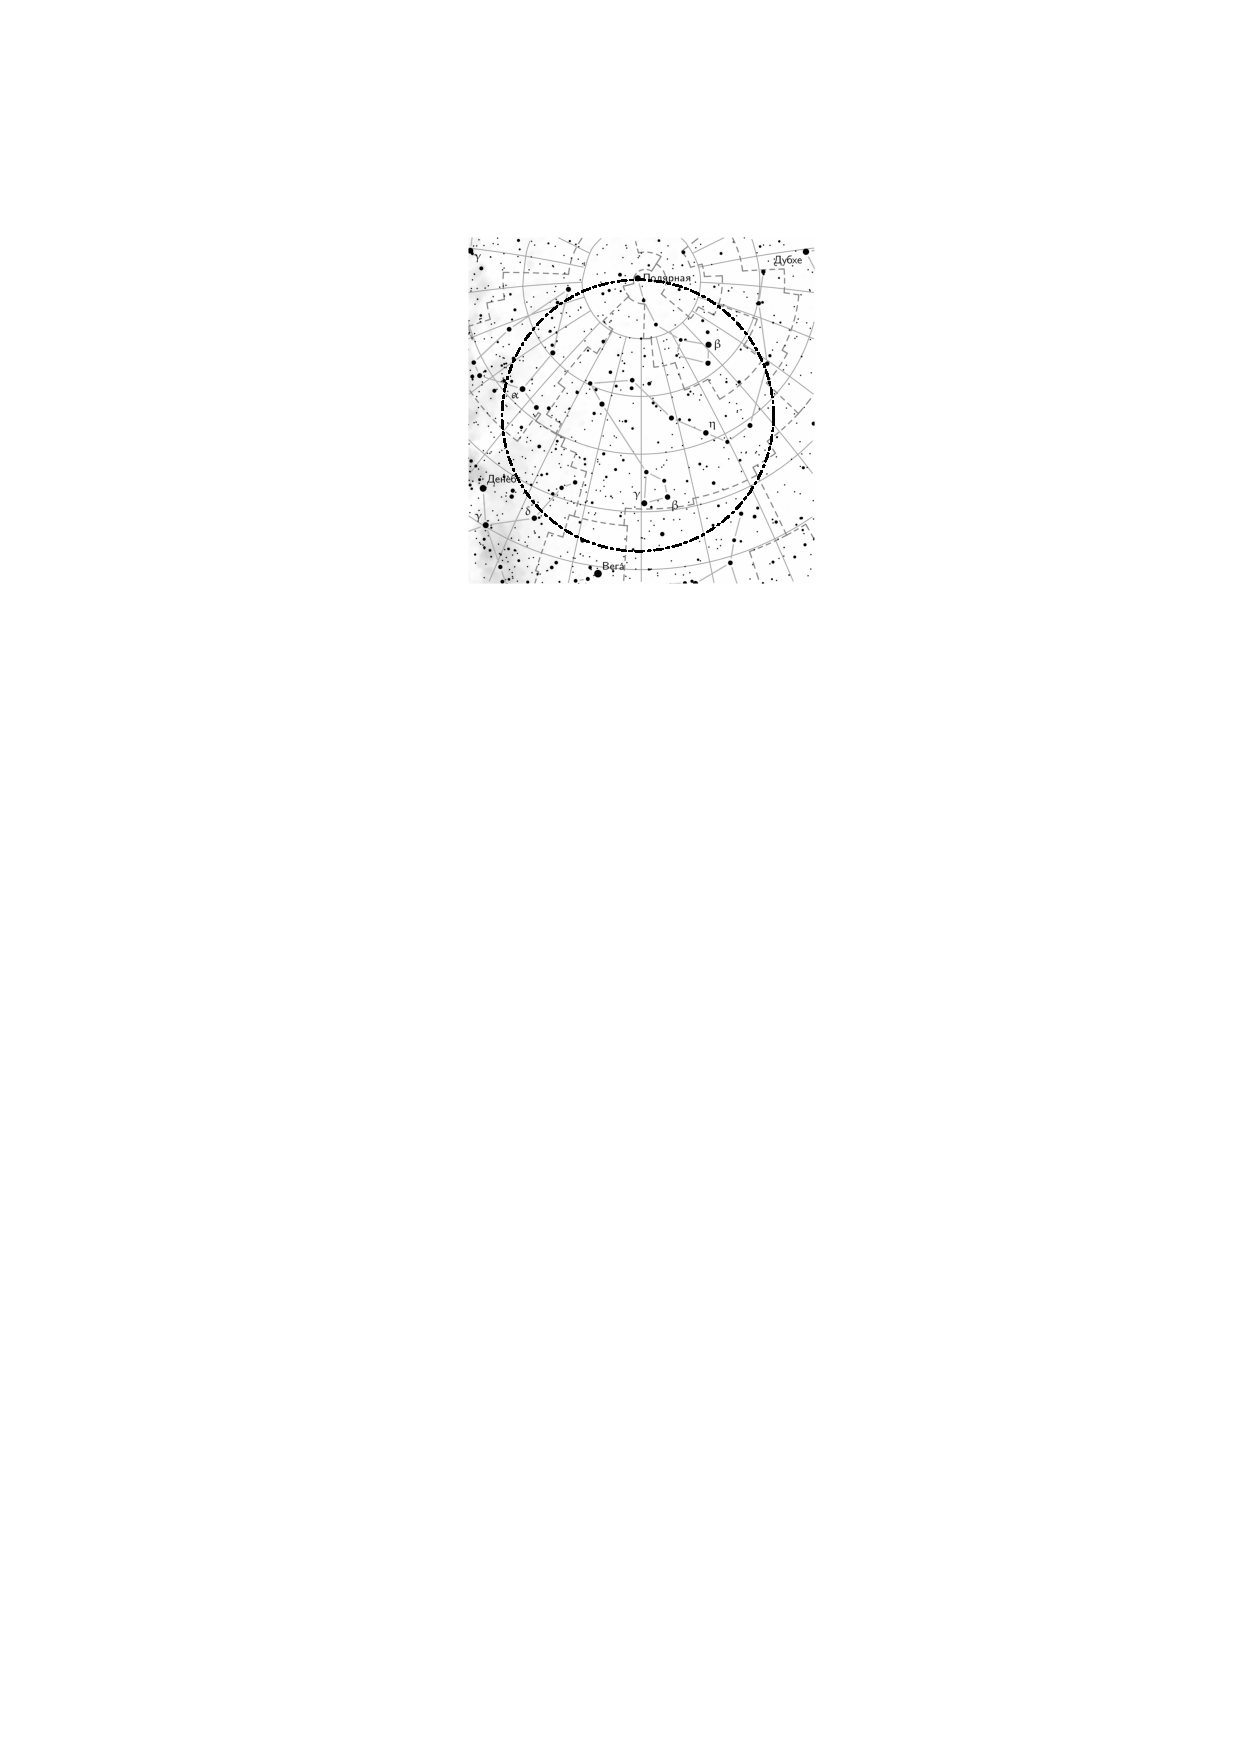
\includegraphics[width = .42\tw]{precession_bw}
	\caption{Прецессионное движение северного полюса мира}
	\label{fig:precession-path}
\end{wrapfigure}
Под действием возмущающих сил ось вращения Земли совершает прецессионное движение: описывает вокруг оси эклиптики конус с углом раствора $23.5^\circ$ с периодом около  25\,765~лет. Из-за этого меняется положение полюс мира. Например, сейчас полюс мира практически совпадает с Полярной звездой ($\alpha$\,UMi), а 15\,000~лет назад роль полярной звезды играла Вега ($\alpha$\,Lyr). Если считать, что величина прецессии постоянна, то полюсы мира описывают вокруг полюсов эклиптики малые круги с радиусом $23.5^\circ$. В~действительности~же величина прецессии меняется, поэтому путь полюсов мира представляет собой не~окружность, а~спираль.

Поворот оси Земли имеет различные последствия. Во-первых, меняется продолжительность тропического года, он становится примерно на $20$~минут короче звёздного, во-вторых, меняется вид звёздного неба  (см.~Рис.\,\ref{fig:precession-path}).

	\section{Конические сечения}
\subsection{Эллипс}

{\bfseries \term{Эллипс}}~--- плоская замкнутая кривая, сумма расстояний от любой точки которой до двух фиксированных точек, называемых фокусами, постоянна.
\begin{equation}
	|F_1 M| + |F_2 M|=\const \label{eq:ell-def}
\end{equation}
\imp{Центром} эллипса называется середина отрезка, соединяющего его фокусы.

\imp{Большая ось} эллипса~--- прямая, проходящая через фокусы эллипса; \imp{малая ось}~--- прямая ей перпендикулярная и проходящая через центр эллипса.

\begin{wrapfigure}[10]{r}{0.5\tw}
	\vspace{-1pc}
	\centering
	\begin{tikzpicture}[ipe stylesheet, scale=0.8]
		\draw[shift={(-65.623, 0.044)}, xscale=0.6567, yscale=0.6949]
		(0, 0)
		-- (0.105, -111.963);
		\draw[shift={(-65.623, 0.044)}, xscale=0.6567, yscale=0.6949, ipe pen heavier]
		(0, 0)
		-- (199.948, 49.784);
		\draw[shift={(-65.623, 0.044)}, xscale=0.6567, yscale=0.6949, ipe pen heavier]
		(0, 0)
		-- (100, -80);
		\draw[ipe pen fat]
		(0.0497, 0.0443) ellipse[x radius=84.0612, y radius=55.5917];
		\draw[shift={(-84.012, 0.044)}, xscale=0.6567, yscale=0.6949, ipe pen heavier]
		(0, 0)
		-- (256, 0);
		\draw[shift={(0.05, 55.636)}, xscale=0.6567, yscale=0.6949, ipe pen heavier]
		(0, 0)
		-- (0, -160);
		\pic[ipe mark small, fill=white]
		at (-65.6232, 0.0443) {ipe fdisk};
		\draw[shift={(65.723, 0.044)}, xscale=0.6567, yscale=0.6949, ipe pen heavier]
		(0, 0)
		-- (0.012, 49.938);
		\draw[shift={(0.05, 55.636)}, xscale=0.6567, yscale=0.6949]
		(0, 0)
		-- (-144, 0);
		\draw[shift={(0.05, -55.547)}, xscale=0.6567, yscale=0.6949]
		(0, 0)
		-- (-144, 0);
		\draw[shift={(-84.012, 0.044)}, xscale=0.6567, yscale=0.6949]
		(0, 0)
		-- (-16, 0);
		\draw[shift={(84.111, 0.044)}, xscale=0.6567, yscale=0.6949]
		(0, 0)
		-- (16, 0);
		\draw[shift={(65.733, 34.723)}, xscale=0.6567, yscale=0.6949]
		(0, 0)
		-- (43.975, 0.069);
		\draw[shift={(89.365, 0.044)}, xscale=0.6567, yscale=0.6949, {ipe fptarc[ipe arrow small]}-{ipe fptarc[ipe arrow small]}]
		(0, 0)
		-- (0.028, 49.882);
		\node[ipe node]
		at (90.524, 16.168) {$p$};
		\draw[shift={(-89.265, 55.636)}, xscale=0.6567, yscale=0.6949, {ipe fptarc[ipe arrow small]}-{ipe fptarc[ipe arrow small]}]
		(0, 0)
		-- (0, -80);
		\draw[shift={(-89.265, 0.044)}, xscale=0.6567, yscale=0.6949, {ipe fptarc[ipe arrow small]}-{ipe fptarc[ipe arrow small]}]
		(0, 0)
		-- (0, -80);
		\draw[shift={(-84.012, 0.044)}, xscale=0.6567, yscale=0.6949]
		(0, 0)
		-- (0, -104);
		\draw[shift={(0.05, -55.547)}, xscale=0.6567, yscale=0.6949]
		(0, 0)
		-- (0, -16);
		\draw[shift={(84.252, 0.195)}, xscale=0.6567, yscale=0.6949]
		(0, 0)
		-- (0, -112);
		\node[ipe node]
		at (66.165, -9.39) {\bf F$_\mathbf{2}$};
		\draw[shift={(-84.012, -66.531)}, xscale=0.6567, yscale=0.6949, {ipe fptarc[ipe arrow small]}-{ipe fptarc[ipe arrow small]}]
		(0, 0)
		-- (28, 0);
		\draw[shift={(-65.545, -61.052)}, xscale=0.6567, yscale=0.6949, {ipe fptarc[ipe arrow small]}-{ipe fptarc[ipe arrow small]}]
		(0, 0)
		-- (99.881, -0.078);
		\draw[shift={(0.05, -61.107)}, xscale=0.6567, yscale=0.6949, {ipe fptarc[ipe arrow small]}-{ipe fptarc[ipe arrow small]}]
		(0, 0)
		-- (128, 0);
		\draw[shift={(-65.501, -72.162)}, xscale=0.6567, yscale=0.6949, {ipe fptarc[ipe arrow small]}-{ipe fptarc[ipe arrow small]}]
		(0, 0)
		-- (227.814, -0.09);
		\node[ipe node]
		at (-94.935, 25.494) {$b$};
		\node[ipe node]
		at (-94.808, -30.216) {$b$};
		\node[ipe node]
		at (-77.03, -72.327) {$q$};
		\node[ipe node]
		at (-33.24, -67.42) {$c$};
		\node[ipe node]
		at (40.523, -67.405) {$a$};
		\node[ipe node]
		at (5.465, -80.93) {$Q$};
		\draw[shift={(0.05, -55.547)}, xscale=0.6567, yscale=0.6949, ipe pen heavier]
		(0, 0)
		-- (100, 80);
		\node[ipe node]
		at (-29.49, -28.163) {$a$};
		\node[ipe node]
		at (26.538, -27.093) {$a$};
		\node[ipe node]
		at (-30.549, 19.559) {$2a-p$};
		\pic[ipe mark small, fill=white]
		at (0.0497, 0.0443) {ipe fdisk};
		\node[ipe node]
		at (-10.329, -9.706) {\bf O};
		\pic[ipe mark small, fill=white]
		at (65.7225, 0.0443) {ipe fdisk};
		\node[ipe node]
		at (-78.578, -8.924) {\bf F$_\mathbf{1}$};
		\pic[ipe mark small, fill=white]
		at (65.7527, 34.68) {ipe fdisk};
		\pic[ipe mark small, fill=white]
		at (-84.0076, 0.0853) {ipe fdisk};
		\pic[ipe mark small, fill=white]
		at (0.0044, -55.5391) {ipe fdisk};
		\pic[ipe mark small, fill=white]
		at (84.1418, 0.0783) {ipe fdisk};
		\pic[ipe mark small, fill=white]
		at (0.0208, 55.6916) {ipe fdisk};
	\end{tikzpicture}
	\captionof{figure}{Эллипс}
	\label{pic:ellipse}
\end{wrapfigure}
Главные отрезки эллипса: \term{большая полуось} ($a$)~--- расстояние от центра эллипса до его пересечения с большой осью; \term{малая полуось} ($b$) определяется дословно также, заменив большую ось на малую; \term{фокальное расстояние} ($c$)~--- расстояние от центра эллипса до одного из фокусов, что тоже самое, половина расстояния между фокусами.

Рассмотрим крайнюю левую и крайнюю правую точки эллипса на Рис.~\ref{pic:ellipse}, назовем их $A$ и $B$ соответственно, тогда сумма расстояний $l$ от каждой из них до фокусов $F_1$ и $F_2$ равна:
\begin{equation*}
	AF_1 + AO + OF_2 = AF_1 + a + c = l = BF_2 + BO + OF_1 = BF_2 + a + c.
\end{equation*}
Откуда следует, что $A F_1 = B F_2$. Легко видеть, что $AB = 2a$, значит $l = AF_1 + AO + OF_2 = AO + OF_2 + F_2B = 2a$. Получается, сумма расстояний до фокусов от любой точки эллипса равна его удвоенной большой полуоси.

В силу равенства прямоугольных треугольников $\triangle F1 O C$ и $\triangle F_2 O C$ равны их гипотенузы $F_1C$ и $F_2C$, причем $F_1C= F_2C = l/2 = a$. Отсюда получается одно из основных соотношений в эллипсе:

\begin{equation}
	b^2 + c^2 = a^2.
\end{equation}
\term{Эксцентриситет} ($e$)~--- числовая
характеристика, показывающая степень отклонения конического сечения от окружности. Для эллипса $e$ лежит в интервале $(0, \, 1)$ и
определяется формулой
\begin{equation}
	e = \frac{c}{a}.
\end{equation}

\term{Апоцентр}~--- наиболее удаленная от заданного фокуса точка эллипса. Расстояние $Q$ до апоцентра от фокуса~--- сумма расстояний от фокуса, до центра эллипса и расстояния от центра до апоцентра, т.\,е.

\begin{equation}
	Q = c + a = a (1 + e).
\end{equation}

\term{Перицентр}~--- ближайшая точка эллипса к заданному фокусу. По аналогии с апоцентром, для расстояния $q$ от фокуса эллипса до перицентра справедливо следующее:
\begin{equation}
	q = a - c = a (1 - e).
\end{equation}

\term{Фокальный параметр}~($p$)~--- длина перпендикуляра, проведенного из фокуса до точки пересечения с эллипсом. Найдем $p$ из теоремы Пифагора для треугольника $\triangle F_1 F_2 P$:
\begin{gather}
	p^2 = (2a - p)^2 - (2c)^2, \notag\\
	p^2 =  4a^2 - 4ap + p^2 - 4a^2e^2,\notag\\
	0 = a ( 1 - e^2) - p,\notag\\
	p = a (1 - e^2) = \frac{b^2}{a} = b \sqrt{1 - e^2}.
\end{gather}

Получим теперь выражение для расстояния от произвольной точки эллипса с \term{истинной аномалией}~$\nu$~--- угол
{\slshape перицентр -- фокус -- заданная точка},
отсчитываемый в сторону движения по эллипсу. Для этого необходимо рассмотреть треугольник {\slshape перицентр -- фокус -- заданная точка} и записать для него теорему косинусов:
\begin{gather*}
	(2a - r)^2 = r^2 + (2c)^2 - 2 r \cdot 2c \cos (180^\circ - \nu),\\
	4a^2 - 4ar + r^2 = r^2 + 4 a^2 e^2 + 4 r a e \cos \nu,\\
	a - r = ae^2 + re\cos \nu,\\
	r = \frac{a(1 - e^2)}{1 + \cos \nu}.
\end{gather*}
Полученное выражение для длины радиус-вектора точки на эллипсе в зависимости от ее угла от перицентра называется \term{уравнением эллипса в полярных координатах}. Если же полюс системы координат расположить в другом фокусе, тогда полярный угол будет, очевидно, отсчитываться от точки апоцентра и в знаменателе уравнения будет знак <<$-$>>. Окончательно,
\begin{equation}
	r = \frac{a ( 1- e^2)}{1 \pm e \cos \nu}.
	\label{eq:ell-eq-pol}
\end{equation}

Перейдем теперь в декартовы координаты, в которых $r = \sqrt{x^2 + y^2}$, а $\cos \nu = x / r$, тогда:
\begin{gather*}
	\sqrt{x^2 + y^2} = \frac{a(1 - e^2)}{1 + e \cdot \dfrac{x}{\sqrt{x^2 + y^2}}} = \frac{a (1 - e^2) \sqrt{x^2 + y^2}}{\sqrt{x^2 + y^2} + e x},\\
	\sqrt{x^2 + y^2} = a(1 - e^2) - e x,\\
	x^2 + y^2 = a^2 (1 - e^2)^2 + e^2 x^2 - 2ae(1 - e^2) x,\\
	(1 - e^2) x^2 + y^2 = a^2 (1 - e^2)^2 - 2ae (1 - e^2) x,\\
	x^2 + \frac{y^2}{1 - e^2} = a^2 (1 - e^2) - 2aex.
\end{gather*}
Сдвинем систему отсчета влево так, чтобы центр эллипса оказался в начале координат, тогда новая координата по оси $x$ определяется, как $\xi = x + ae$, иначе $x = \xi - ae$. Подставим полученное выражение в преобразованное уравнение:
\begin{gather*}
	\xi^2 + a^2 e^2 - 2ae\xi + \frac{y^2}{1 - e^2} = a^2 (1 - e^2) - 2 ae\xi + 2 a^2 e^2,\\
	\xi^2 + a^2 e^2  + \frac{y^2}{1 - e^2} = a^2 - a^2 e^2 + 2 a^2 e^2,\\
	\frac{\xi^2}{a^2} + \frac{y^2}{a^2 (1 - e^2)} = 1,\\
	\frac{\xi^2}{a^2} + \frac{y^2}{b^2} = 1. \tag{\theequation} \label{eq:ell-eq-dec}
\end{gather*}
Данное уравнение называется \term{уравнением эллипса в декартовых координатах}.

Далее покажем, что любая точка плоскости, удовлетворяющая \eqref{eq:ell-eq-dec} принадлежит эллипсу с большой полуосью $a$ и малой~--- $b$, чтобы доказать равносильность предыдущих переходов. Для этого выберем произвольную точку $(x_0, y_0)$, для которой выполняется \label{eq:ell-eq-dec}, т.\,е.
\begin{equation}
	y_0 = \pm b \sqrt{1 - \frac{x_0^2}{a^2}} = \pm \sqrt{1 - e^2} \sqrt{a^2 - x_0^2}. \label{eq:ell-y0}
\end{equation}
Докажем, что множество точек $(x_0, y_0)$, для которых справедливо равенство \eqref{eq:ell-y0} являются эллипсом, а точки $(\pm a e, 0)$~--- его фокусами:
\begin{multline*}
	r_{1,2}
	= \big| (x_0, y_0) - (\pm ae, 0) \big|
	= \sqrt{(x_0 \mp ae)^2 + y_0^2} =\\
	= \sqrt{x_0^2 \mp 2 a e x_0 + a^2 e^2 + a^2(1 - e^2) - x_0^2(1 - e^2)} =\\
	= \sqrt{x_0^2 \mp 2 a e x_0 + a^2 e^2 + a^2 - a^2 e^2 - x_0^2 + e^2 x_0^2} = \\
	= \sqrt{e^2 x_0 \mp 2 a e x_0 + a^2 } = \sqrt{(e x_0 \mp a)^2} = |e x_0 \mp a| = a \mp ex_0.
\end{multline*}
Отсюда получается, что $r_1 + r_2 = 2a$, а значит рассмотренное множество точек, удовлетворяет определению эллипса. Это доказывает эквивалентность определений эллипса в виде \eqref{eq:ell-def}, \eqref{eq:ell-eq-pol} и \eqref{eq:ell-eq-dec}.

Теперь легко показать, что эллипс является образом афинного преобразования сжатия окружности с радиусом $a$. Для этого рассмотрим окружность, задаваемую уравнением $x^2 + y^2 = a^2$ и сжатие вдоль оси $y$ с коэффициентом $1/\sqrt{1 - e^2}$. Тогда $x' \hookrightarrow x$, а $y' \hookrightarrow y \sqrt{1-e^2}$. Следовательно для обратного преобразования $x \hookrightarrow x'$, а $y \hookrightarrow y'/\sqrt{1 - e^2}$. При этом прообраз сжатой окружность должен быть исходной окружность, а значит, удовлетворять исходному уравнения, то есть
\begin{gather*}
	x'^2 + \frac{y'^2}{1 - e^2} = a^2,\\
	\frac{x'^2}{a^2} + \frac{y'^2}{b^2} = 1.
\end{gather*}
Получаем, что образ окружности под действием афинного преобразования сжатия является эллипсом.

Данный факт помогает легко найти \term{площадь эллипса}~($S$)~--- площадь части
плоскости, ограниченной эллипсом. Так как под действием сжатия площади уменьшаются пропорционально коэффициенту преобразования, что есть
\begin{equation}
	S = S_\text{окр} \sqrt{1 - e^2} = \pi a^2 \sqrt{1 - e^2} = \pi a b.
\end{equation}

Также из свойств афинного преобразования и параметрического уравнения окружности следует \imp{параметрическое уравнение эллипса}, которое имеет такой вид:
\begin{equation}
	\left\{
	\begin{aligned}[lcl]
		&x=a\cos t,\\
		&y=b\sin t;\\
	\end{aligned}
	\right. \quad\quad t \in [0, \, 2\pi).
\end{equation}

Кроме этого, эллипс обладает важным \imp{оптическим свойством}, которое можно сформулировать так: свет от источника в одном из фокусов, отражается эллипсом так, что отражённые лучи пересекаются во втором фокусе или, что тоже самое, касательная к эллипсу в заданной точке образует с фокальными радиусами в данной точке равные острые углы. Для его доказательства необходимо показать равенство углов между касательной в точке к эллипсу и направлениями на фокусы. Для этого получим сначала уравнение касательной к эллипсу в произвольной точке $(x_0, y_0$, принадлежащей ему. Как было показано выше, эллипс можно представить объединением графиков двух функций \eqref{eq:ell-y0}. Найдем теперь производные от этих функций по $x_0$:
\begin{equation*}
	(y_0)'_{x_0} = \pm \sqrt{1 - e^2} \cdot \frac{-x_0}{\sqrt{a^2 - x_0^2}}.
\end{equation*}
Так как значение производной в точке равно тангенсу угла наклона касательной, то направляющий вектор касательной можно представить в виде $\vec{t} = \left(1,  (y_0)'_{x_0}\right)$, иначе:
\begin{equation*}
	\vec t =
	\begin{pmatrix}
		1\\
		\mp \sqrt{1 - e^2} \cdot \dfrac{\alpha}{\sqrt{1 - \alpha^2}}
	\end{pmatrix},~\text{где}~ \alpha \equiv \frac{x_0}{a},\quad -1 \leqslant \alpha \leqslant 1.
\end{equation*}
При этом модуль направляющего вектора $\vec t$ определяется, как
\begin{equation*}
	|\vec t| \equiv t = \sqrt{t_x^2 + t_y^2} = \sqrt{1 + (1 - e^2) \cdot \frac{\alpha^2}{1 - \alpha^2}} = \sqrt{\frac{1 - e^2 \alpha^2}{1 - \alpha^2}}.
\end{equation*}
Выпишем векторы $\vec r_1$ и $\vec r_2$, от точки $(x_0, y_0)$ до фокусов, имеющих координаты $(\pm ae, 0)$ соответственно:
\begin{equation*}
	\vec r_{1,2} =
	\begin{pmatrix}
		\pm ae - x_0\\
		-y_0
	\end{pmatrix}.
\end{equation*}
Покажем теперь, что $\cos \widehat{\vec r_1 \vec t} = - \cos \widehat{\vec r_2 \vec t}$ для верхнего полуэллипса, что завершит доказательство оптического свойства эллипса, так как для нижнего доказательство аналогично:
\begin{multline*}
	\cos \widehat{\vec r_{1, 2}  \vec t}
	= \frac{(r_{1, 2}, t)}{|\vec r_{1, 2}| | \vec t|} = \\
	= \frac{(\pm ae - x_0) \cdot 1 + \left[ -y_0 \cdot \left(- \sqrt{1 - e^2} \cdot \dfrac{\alpha}{\sqrt{1 - \alpha^2}} \right) \right]}{\sqrt{(\pm ae - x_0)^2 + y_0^2} \cdot \sqrt{\dfrac{1 - e^2 \alpha^2}{1 - \alpha^2}}} =\\
	= \frac{(\pm ae - x_0) \cdot \sqrt{1 - \alpha^2} + \alpha y_0\sqrt{1 - e^2}}{\sqrt{(\pm ae - x_0)^2 + y_0^2} \cdot \sqrt{1 - e^2 \alpha^2}}.
\end{multline*}
Из параметричекого уравнения эллипса можно получить, что $\sin t = x_0/a = \alpha$, тогда
\begin{equation*}
	y_0 = b \cos t = b \sqrt{1 - \sin^2 t} = b \sqrt{1 - \alpha^2} = a \sqrt{1 - e^2} \sqrt{1 - \alpha^2}.
\end{equation*}
Подставим данное выражение для $y_0$ в предыдущие выкладки:
\begin{multline*}
	\cos \widehat{\vec r_{1, 2}  \vec t}
	= \frac{a ( \pm e - \alpha) \sqrt{1 - \alpha^2} + \alpha a \sqrt{1 - e^2} \sqrt{1 - \alpha^2} \sqrt{1 - e^2}}{a \sqrt{(\pm e - \alpha)^2 + (1 - e^2)(1 - \alpha^2)} \cdot \sqrt{1 - e^2 \alpha^2}} = \\
	= \frac{ (\pm e - \alpha + \alpha - e^2 \alpha) \sqrt{1 - \alpha^2}}{\sqrt{e^2 \mp 2 e\alpha + \alpha^2 + 1 - \alpha^2 - e^2 + e^2 \alpha^2} \cdot \sqrt{1 - e^2 \alpha^2}} = \\
	= \frac{ (\pm e - e^2 \alpha) \sqrt{1 - \alpha^2}}{\sqrt{\mp 2 e\alpha + 1  + e^2 \alpha^2} \cdot \sqrt{1 - e^2 \alpha^2}} = \\
	= \frac{ e(\pm 1 - e \alpha) \sqrt{1 - \alpha^2}}{|1 \mp e\alpha| \sqrt{1 - e^2 \alpha^2}}
	= \frac{ e(\pm 1 - e \alpha) \sqrt{1 - \alpha^2}}{(1 \mp e\alpha) \sqrt{1 - e^2 \alpha^2}}
	= \pm \frac{e \sqrt{1 - \alpha^2}}{\sqrt{1 - e^2 \alpha^2}}.
\end{multline*}


\subsection{Парабола}
{\bfseries \term{Парабола}} --- геометрическое место точек, равноудалённых от данной прямой (называемой \term{директрисой} параболы) и данной точки (называемой \term{фокусом} параболы).

{\itshape Каноническое уравнение параболы}:
\begin{equation}
	y^2=2px,
\end{equation}
где $p$~--- \term{фокальный параметр}, равный расстоянию между фокусом параболы и директрисой или удвоенному расстоянию между фокусом параболы и вершиной.

Парабола в полярной системе координат $(r,\varphi)$ с центром в фокусе и нулевым направлением вдоль оси параболы (от фокуса к вершине) может быть представлена в виде уравнения
\begin{equation}
	r = \frac{p}{1 + \cos\varphi}.
\end{equation}
Эксцентриситет параболы равен $e=1$. Важно отметить, что парабола не имеет \term{большой} и \term{малой полуоси}.

Как и все конические сечения, парабола обладает \textit{оптическим свойством}, которое формулируется следующим образом: пучок лучей, параллельных оси параболы, отражаясь в параболе, собирается в её фокусе. И наоборот, свет от источника, находящегося в фокусе, отражается параболой в пучок параллельных её оси лучей.

\subsection{Гипербола}
 
{\bfseries \term{Гипербола}} --- геометрическое место точек евклидовой плоскости, абсолютное значение разности расстояний от которых до двух выделенных точек $F_1$ и $F_2$, называемых фокусами, постоянно и равно удвоенной действительной полуоси гиперболы.
\begin{equation}
\bigl||F_1M|-|F_2M|\bigr| = 2a
\end{equation}

\begin{wrapfigure}[14]{r}{0.5\tw}
	\vspace{-1pc}
	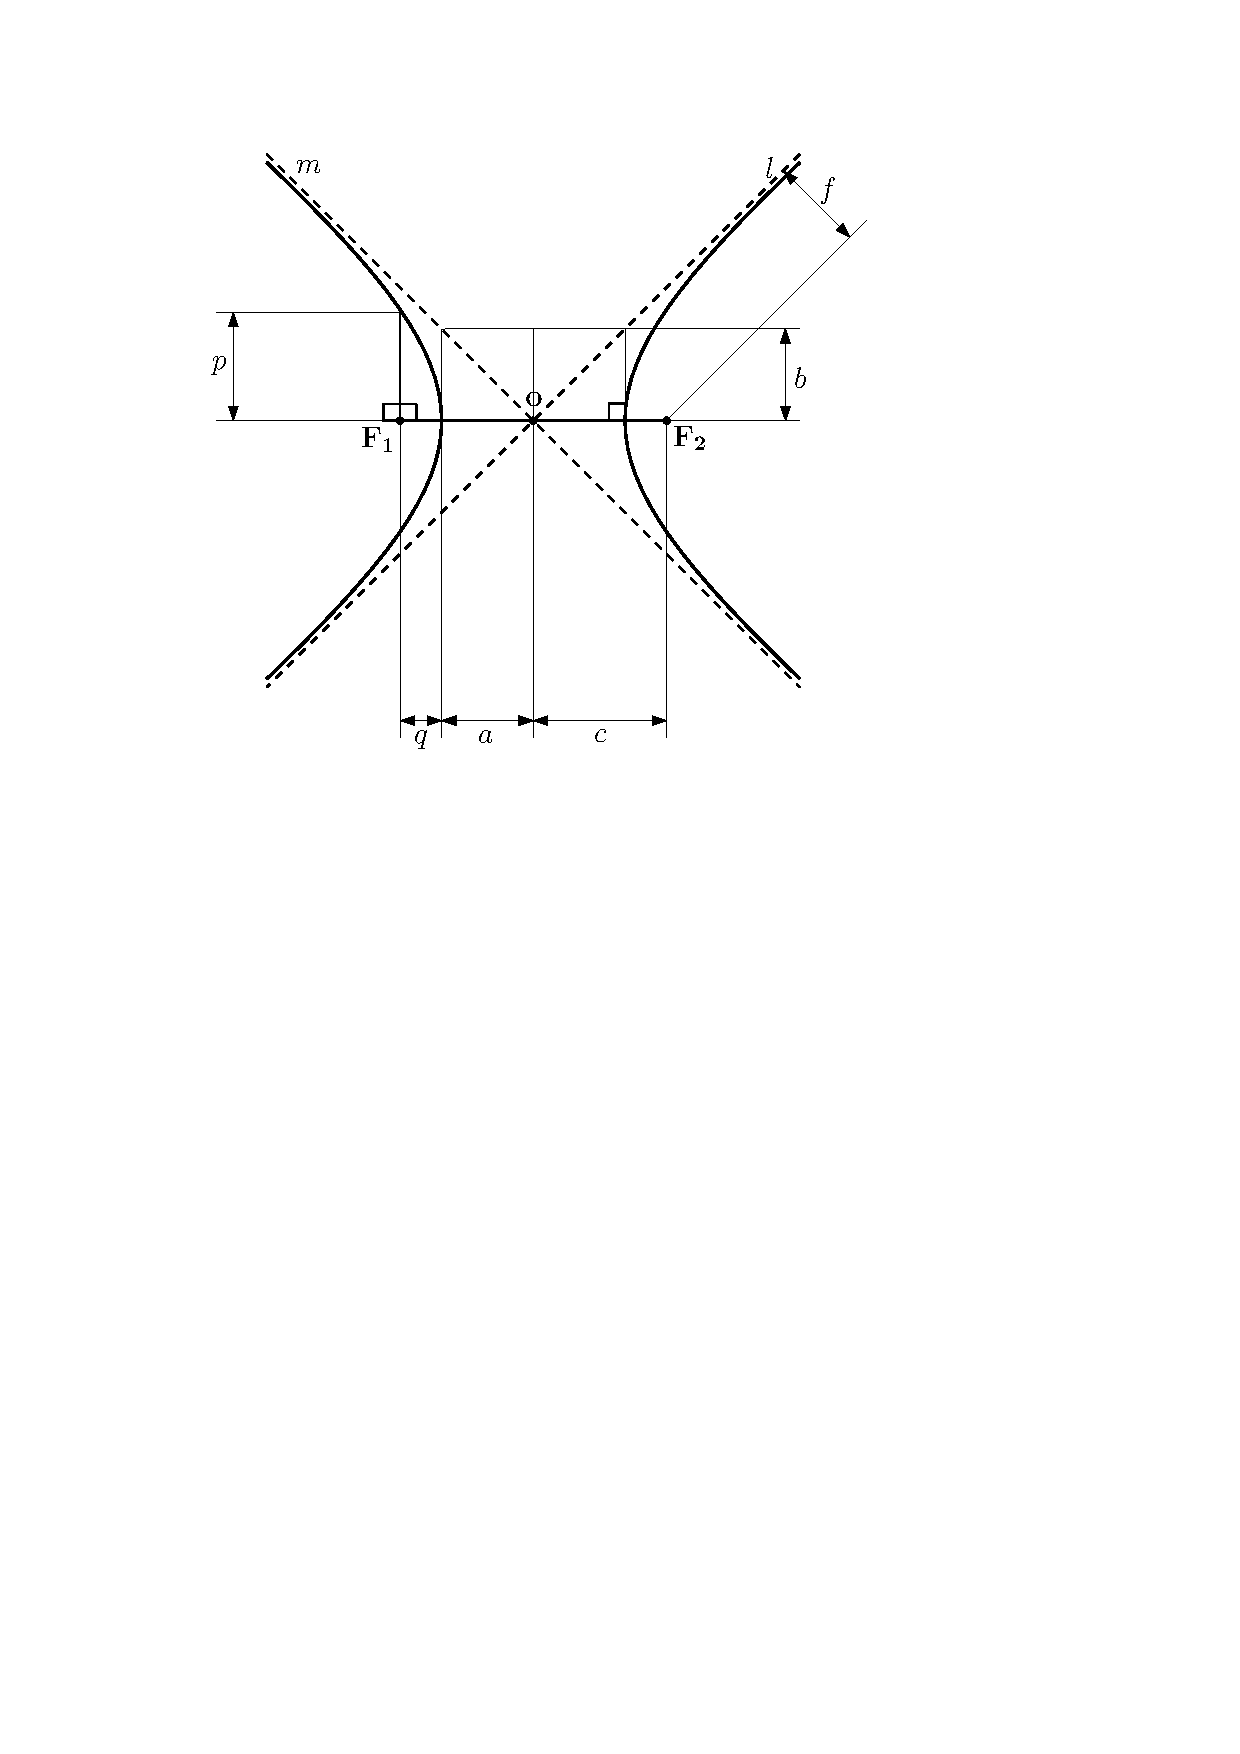
\includegraphics[width = 0.5\textwidth]{Hiperbola}
	\captionof{figure}{Гипербола \label{pic:the-pic}}
\end{wrapfigure}
Ближайшие друг к другу точки двух ветвей гиперболы называются \term{вершинами} гиперболы. \term{Большая} или \term{действительная полуось}~($a$) гиперболы~--- расстояние от центра гиперболы до одной из вершин. \term{Фокальное расстояние}~($c$)~---  расстояние от центра гиперболы до одного из фокусов. \term{Эксцентриситетом} гиперболы~($e$), как и  эллипса, является отношение фокального расстояния к большой полуоси, так как большая полуось гиперболы всегда меньше её фокального расстояния, эксцентриситет гиперболы $e > 1$ и может быть найдет из определения:
\begin{equation}
e=\frac{c}{a}.
\end{equation}

\term{Перицентрическое расстояние} ($q$) --- расстояние от фокуса до ближайшей вершины гиперболы, можно найти, как
\begin{equation}
q = a ( e - 1).
\end{equation}
\term{Мнимая полуось}~($b$)~--- длина перпендикуляра к оси абсцисс, восставленного из вершины до пересечения с асимптотой. Равна \term{прицельному параметру}~($f$)~--- расстоянию от фокуса до асимптоты гиперболы.

\term{Фокальный параметр}~($p$)~--- длина отрезка, перпендикулярного к действительной оси, проведённого от фокуса до гиперболы. Определяется формулой
\begin{equation}
p=\frac{b^2}{a}.
\end{equation}

\imp{Каноническое уравнение гиперболы} в прямоугольных декартовых координатах записывается следующим образом:
\begin{equation}
\frac{x^2}{a^2}-\frac{y^2}{b^2}=1.
\end{equation}
В \imp{полярных координатах} уравнение принимает вид:
\begin{equation}
r=\frac{p}{1-e\cos\varphi},
\end{equation}
причём полюс находится в фокусе гиперболы, а вершина гиперболы лежит на продолжении полярной оси.

\imp{Уравнение двух асимптот} является уравнением пересекающихся прямых:
\begin{equation}
	\frac{x}{a}\pm\frac{y}{b}=0.
\end{equation}

Важным соотношением для элементов гиперболы является
\begin{equation}
c^2=a^2+b^2.
\end{equation}
Также, как и любое коническое сечение, гипербола имеет своё {\itshape оптическое свойство}: свет от источника, находящегося в одном из фокусов гиперболы, отражается второй ветвью гиперболы таким образом, что продолжения отраженных лучей пересекаются во втором фокусе.

	\newpage
\section{Астрофизика}
\subsection{Звёздные величины}
Звёздная величина~--- безразмерная числовая характеристика яркости объекта. Принято, что увеличению светового потока в 100 раз соответствует уменьшение звёздной величины ровно на 5 единиц. Тогда уменьшение звёздной величины на одну единицу означает увеличение плотности светового потока в $\sqrt[5]{100}\approx 2.512$~раз, то есть звёздные величины являются логарифмической шкалой измерения плотности потока. Зависимость, связывающая отношение освещённостей $E_1$ и $E_2$ и разность звёздных величин $m_1$ и $m_2$ двух объектов, называется \term{формулой Погсона} и имеет вид
\begin{equation}
    \frac{E_1}{E_2} = 10^{0.4(m_2 - m_1)} \quad \text{или} \quad m_2 = m_1 + 2.5 \lg \frac{E_1}{E_2}.
    \label{eq:pogson-law}
\end{equation}

Широко используется понятие \term{абсолютной звёздной величины} $M$~--- это звёздная величина при наблюдении с установленного расстояния~$R_0$: для звёзд и объектов вне Солнечной системы~---~10~пк, для тел Солнечной системы~---~1~\au, причем считается, что тело находится в 1~\au~и от наблюдателя и от Солнца, а фаза равна единице, то есть можно считать, что наблюдатель находится в центре Солнца, а~тело~--- в~1~\au~от него.

Абсолютную звёздную величину объекта вне Солнечной системы можно получить по формуле Погсона \eqref{eq:pogson-law} из наблюдаемой звёздной величины~$m$ и расстояния~$r$ до него
\begin{equation}
    M = m + 2.5 \lg \frac{E}{E_\text{абс}} = m + 2.5 \lg \frac{L \cdot R_0^2}{r^2 \cdot L} = m + 5 \lg \frac{R_0}{r}.
    \label{eq:absolute-magnutude}
\end{equation}
Если принимать к рассмотрению межзвездное поглощение~$A$, то формулу  \eqref{eq:absolute-magnutude} необходимо уточнить:
\begin{equation}
    M = m + 5 \lg \frac{R_0}{r} - Ar.
\end{equation}

Важно определить понятие \term{болометрической звёздной величины}~$m_\text{bol}$~--- это звёздная величина, при расчёте которой учитывается полная мощность излучения источника во всем диапазоне длин электромагнитных волн.

Резолюция B2, принятая на Генеральной Асамблеи Международного астрономического союза в 2015 году\,\cite{bolometric-magnitude}, определяет нуль-пункт звёздных величин. Так \imp{абсолютную болометрическую звёздную величину}, равную $0^m$ имеет изотропный источник излучения с мощностью $L_0 = 3.0128 \cdot 10^{28}$~Вт. Данное значение выбрано таким образом, чтобы абсолютная болометрическая звёздная величина Солнца $M_{\text{Bol}\odot}$ составляла $4.74^m$. Такому источнику излучения соответствует наблюдаемая плотность потока
\begin{equation}
    E_0 = \frac{L_0}{4\pi R_0^2} = 2.518021002\ldots \cdot 10^{-8}~\frac{\text{Вт}}{\text{м}^2}.
\end{equation}
Исходя из этого, используя \imp{формулу Погсона}, можно определить болометрическую звёздную величину любого изотропного источника излучения, зная его светимость и расстояние до него.

\term{Фотометрическая звёздная величина}~--- звёздная величина источника в некотором фильтре $\xi$, для которого определена функция чувствительности приемника $S_\xi(\lambda): [0, +\infty] \rightarrow [0,1]$. Определяется выражением
\begin{equation}
    m_\xi = -2.5\lg \frac{\int E(\lambda) S_\xi(\lambda) \, d \lambda}{E_0} + C_\xi,
\end{equation}
где $E(\lambda)$~--- плотность потока излучения от источника на длине волны~$\lambda$, а $C_\xi$~--- нормировочная константа фильтра $\xi$. Несмотря на то, что интегралы определенные, звёздная величина в том или ином фильтре определяется с точностью до нормировки на определенный нуль-пункт.

\begin{wraptable}[15]{r}{0.43\tw}
    \vspace{-0.75pc}
    \footnotesize
    \centering
    \renewcommand{\arraystretch}{1.2}
    \begin{tabular}{|c|c|c|}
        \hline
        Фильтр & $\langle\lambda\rangle$, нм & FWHM, нм \\
        \hline
        $U$    & 365                         & 66       \\
        $B$    & 445                         & 94       \\
        $V$    & 551                         & 88       \\
        $R$    & 658                         & 138      \\
        $I$    & 806                         & 149      \\
        $Y$    & 1020                        & 120      \\
        $J$    & 1220                        & 213      \\
        $H$    & 1630                        & 307      \\
        $K$    & 2190                        & 390      \\
        $L$    & 3450                        & 472      \\
        $M$    & 4750                        & 460      \\
        $N$    & 10500                       & 2500     \\
        \hline
    \end{tabular}
    \caption{Параметры фильтров фотометрической системы Джонсона}
    \label{tbl:johnson-bands}
\end{wraptable}
Для стандартизации фотометрических звёздных величин описаны различные фотометрические системы, особенно распространена система, опубликованная в 1966 году\,\cite{johnson-photometry}, где авторы определяют 8 широкополосных фильтров $U\!BV\!RIJKL$ (позднее были добавлены фильтры $M$ и $N$), параметры которых приведены в Таблице\,\ref{tbl:johnson-bands}, а профили пропускания представлены на \picRef{pic:johnson-bands}. Нуль-пунктом отсчета звездной величины в каждом из фильтров является блеск звезды спектрального класса $A0V$~--- Веги ($\alpha$\,Lyr), которой принимается равным $0.03^m$ в каждом из фильтров.

\begin{figure}[t]
    \centering
    \begin{subcaptionblock}{\tw}
        \centering
        \tikzsetnextfilename{johnson-bands-1}
        \begin{tikzpicture}
            \begin{axis} [
                width   =    \tw,
                height  =    3.5cm,
                xmax    =    1500,
                xmin    =    300,
                xlabel  =    {Длина волны $\lambda$,~нм},
                ylabel  =    {$S_\xi(\lambda)$}
            ]
                \addplot[black, smooth] table[x=l, y=U] {data/filters-data-U.txt} node at (axis cs:350, 0.5) {\scriptsize{$U$}};
                \addplot[black, smooth] table[x=l, y=B] {data/filters-data-B.txt} node at (axis cs:440, 0.5) {\scriptsize{$B$}};
                \addplot[black, smooth] table[x=l, y=V] {data/filters-data-V.txt} node at (axis cs:550, 0.5) {\scriptsize{$V$}};
                \addplot[black, smooth] table[x=l, y=R] {data/filters-data-R.txt} node at (axis cs:700, 0.5) {\scriptsize{$R$}};
                \addplot[black, smooth] table[x=l, y=I] {data/filters-data-I.txt} node at (axis cs:870, 0.5) {\scriptsize{$I$}};
                \addplot[black, smooth] table[x=l, y=J] {data/filters-data-J.txt} node at (axis cs:1250, 0.5) {\scriptsize{$J$}};
            \end{axis}
        \end{tikzpicture}
    \end{subcaptionblock}
    
    \vspace{0.5pc}
    \begin{subcaptionblock}{\tw}
        \centering
        \tikzsetnextfilename{johnson-bands-2}
        \begin{tikzpicture}
            \begin{axis} [
                width   =    \tw,
                height  =    3.5cm,
                xmax    =    15,
                xmin    =    1,
                xlabel  =    {Длина волны $\lambda$,~мкм},
                ylabel  =    {$S_\xi(\lambda)$}
            ]
                \addplot[black, smooth] table[x=l, y=K] {data/filters-data-K.txt} node at (axis cs:2.2, 0.5) {\scriptsize{$K$}};
                \addplot[black, smooth] table[x=l, y=L] {data/filters-data-L.txt} node at (axis cs:3.5, 0.5) {\scriptsize{$L$}};
                \addplot[black, smooth] table[x=l, y=M] {data/filters-data-M.txt} node at (axis cs:5, 0.5) {\scriptsize{$M$}};
                \addplot[black, smooth] table[x=l, y=N] {data/filters-data-N.txt} node at (axis cs:10, 0.5) {\scriptsize{$N$}};
            \end{axis}
        \end{tikzpicture}
    \end{subcaptionblock}
    \caption{Профили пропускания фотометрических фильтров системы $U\!BV\!RIJKLMN$}
    \label{pic:johnson-bands}
\end{figure}

Важно отметить, когда речь идёт звёздной величине без какой-либо кон\-кретизации, обычно имеется в виду видимая звёздная величина, другими словами~--- звёздная величина в фильтре~$V$, и обозначается как~$m_V$ или просто~$m$.

Разность между болометрической и фотометрической звёздными величинами называется \term{болометрической поправкой} (B.C.), которая отличается для разных спектральных классов звёзд и разных фильтров. Болометрическая поправка для фильтра $\xi$ может быть найдена из определения по формуле
\begin{equation}
    \text{B.C.}_\xi = M_\text{Bol} - M_\xi = m_\text{Bol} - m_\xi = 2.5\lg \frac{\int E(\lambda) S_\xi(\lambda) \, d \lambda}{\int E(\lambda)\, d \lambda} + C_\xi - C_\text{Bol},
\end{equation}
где $C_\text{Bol}=0$, если $C_\xi$ была определена с использованием стандарта~$E_0$.


\subsection{Закон Стефана-Больцмана}
\term{Закон Стефана~--- Больцмана} определяет зависимость плотности мощности излучения абсолютно чёрного тела (АЧТ) $u$ от его температуры $T$:
\begin{equation}
	u = a T^4,
\end{equation}
где $a$~--- некая универсальная константа.
Отсюда полная светимость АЧТ с площадью поверхности $S$
\begin{equation}
	L = S \sigma T^4,
	\label{eq:steff-bol-law}
\end{equation}
константа $\sigma$ называется \term{постоянной Стефана-Больцмана}.

Важно отметить, что \imp{закон Стефана-Больцмана}~--- прямое следствие формулы Планка (\ref{eq:plancks-law-nu} -- \ref{eq:plancks-law-lambda}), так как, исходя из физического смысла формулы Планка, справедливы равенства
\begin{multline}
	\sigma T^4 = \int\limits^\infty_0 B(\lambda, T) \,d \lambda \int\limits_0^{\pi/2} \sin \varphi \,d \varphi \int\limits_0^{2\pi} \cos \varphi \,d \theta = \pi \int\limits^\infty_0 B(\lambda, T) \,d \lambda =\\
	= \int\limits^\infty_0 B(\nu, T) \,d \nu \int\limits_0^{\pi/2} \sin \varphi \,d varphi \int\limits_0^{2\pi} \cos \varphi \,d theta = \pi \int\limits^\infty_0 B(\nu, T) \,d \nu.
\end{multline}

Здесь интегрирование ведется в сферических координатах $(\varphi, \theta)$ по телесному углу $d\Omega = d\varphi \cos \varphi d\theta$. А $\sin \varphi$ во втором интеграле отвечает за проекцию единичной площадки на направление излучения. Вычислим данный интеграл, чтобы получить значение постоянной Стефана-Больцмана:
\begin{equation*}
	\sigma T^4 = \pi \int\limits_0^{\infty} \frac{2h\nu^3}{c^2}\cdot \frac{1}{\exp\left(\frac{h\nu}{kT}\right)-1} \,d \nu.
\end{equation*}
Сделаем замену $x = \frac{h \nu}{k T}$, так как $dx = \frac{h}{k T} d\nu$, то
\begin{equation*}
	\sigma T^4 = \frac{2\pi}{c^2}  \int\limits_0^{\infty} \underbrace{\frac{k^3 T^3}{h^2} x^3}_{h\nu^3} \cdot \frac{1}{e^x - 1} \cdot \underbrace{\frac{kT}{h} \,d x}_{d\nu} = \frac{2 \pi k^4 T^4}{c^2 h^3} \int\limits_0^{\infty} \frac{x^3 \,d x}{e^x - 1}.
\end{equation*}
Значение табличного интеграла $\int\limits_0^{\infty} \frac{x^3 \,d x}{e^x - 1}$ равно $\frac{\pi^4}{15}$, откуда
\begin{equation*}
	\sigma = \frac{2 \pi^5 k^4}{15 c^2 h^3} = 5.67 \cdot 10^{-8}~\frac{\text{Вт}}{\text{м}^2 \cdot \text{К}^4}.
\end{equation*}

Для звёзд главной последовательности выполняется соотношение $L \sim M^{\alpha}$, где~$\alpha$~--- коэффициент пропорциональности, который зависит от массы звезды следующим образом:
\begin{align*}
	\alpha &= 2.5,\quad M < 0.5 M_\odot; \\
	\alpha &= 4, \quad 0.5 M_\odot < M < 8 M_\odot;\\
	\alpha &= 2.5, \quad  M > 8 M_\odot.
	%\alpha &= 1, \quad M > 20 M_\odot.
\end{align*}
Также существует примерная зависимость светимости звёзды от её радиуса, имеющая вид  $L\sim R^{5.2}$.

\subsection{Энергия излучения}
\term{Энергия излучения}~--- энергия, переносимая излучением ($Q_e$).\\
\term{Поток излучения}~--- физическая величина, характеризующая мощность, переносимую излучением,
\begin{equation}
	\Phi_e = \frac{d Q_e}{dt}.
\end{equation}
\imp{Теорема Гаусса}: через любую замкнутую поверхность потоки от одинаковых источников равны.

\term{Спектральная плотность потока излучения}~--- поток излучения, приходящийся на малый единичный интервал спектра,
\begin{equation}
	\Phi_{e, \lambda}(\lambda) = \frac{d\Phi_e(\lambda)}{d\lambda}, \quad\quad \Phi_{e, \nu}(\nu) = \frac{d\Phi_e(\nu)}{d\nu} =  \frac{\lambda^2}{c}\Phi_{e, \lambda}(\lambda).
\end{equation}

\term{Объемная плотность энергии излучения}~--- количество энергии на единицу объема
\begin{equation}
	U_e = \frac{d Q_e}{dV}.
\end{equation}

\term{Светимость}~--- величина, представляющая собой световой поток излучения, испускаемого с малого участка светящейся поверхности единичной площади,
\begin{equation}
	M_e = \frac{d \Phi_e}{dS_1},
\end{equation}
здесь $S_1$~--- площадь объекта, испускающего энергию.

\term{Яркость}~--- световой поток, приходящийся на единичный телесный угол, в расчёте на единичную площадку проекции излучающей поверхности на картинную плоскость,
\begin{equation}
	L_e = \frac{d^2 \Phi_e}{d \Omega\,dS_1 \cos \varepsilon},
\end{equation}
где $\varepsilon$~--- угол между направлением потока излучения и нормалью к плоскости излучающей поверхности.

\term{Интегральная яркость}~--- интеграл яркости по видимой поверхности источника. Показывает количество энергии, пришедшее от источника за единицу времени.
\begin{equation}
	\Lambda_e = \int \limits_S L_e(\vec{r})\,ds.
\end{equation}
\term{Освещенность}~--- величина, равная отношению светового потока, падающего на малый участок поверхности, к его площади~--- поверхностная плотность потока
\begin{equation}
	E_e = \frac{d\Phi_e}{dS_2} \sim \frac{1}{r^2},
\end{equation}
здесь $S_2$~--- площадь поверхности приёмника, $r$~--- расстояние от источника.

\subsection{Альбедо}
\term{Альбедо}~($A$)~--- характеристика отражательной способности поверхности какого-либо объекта. Альбедо является отношением отражённого светового потока к падающему на поверхность объекта. Тогда для нахождения поглощённой части излучения используется соотношение
\begin{equation}
    E_\text{п} = E_0 \cdot (1-A),
\end{equation}
где $E_{\text{п}}$~--- поглощённая часть излучения, $E_0$~--- пришедшее излучение, $A$~--- альбедо. А для отражённой части излучения $E_{\text{отр}}$ можно использовать формулу
\begin{equation}
    E_{\text{отр}}= A \cdot E_0.
\end{equation}

Существует несколько видов альбедо: \imp{геометрическое}, \imp{сферическое} и \imp{бондовское}. \term{Геометрическое альбедо} равно отношению освещённости у Земли, создаваемой планетой в полной фазе, к освещённости, которую создал бы плоский абсолютно белый экран того же размера, что и планета, расположенный на её месте перпендикулярно лучу зрения и солнечным лучам. \term{Сферическое альбедо} определяется как отношение светового потока, рассеянного телом во всех направлениях, к потоку, падающему на это тело. Может быть определено как для некоторого диапазона длин волн, так и для всего спектра. Сферическое альбедо для всего спектра излучения называется \term{альбедо Бонда}.

\subsection{Энергия и импульс фотона}
\term{Фотон}~--- материальная, электрически нейтральная частица, квант электромагнитного поля (переносчик электромагнитного взаимодействия). В силу корпускулярно-волнового дуализма, фотон можно рассматривать либо как частицу, либо как волну. Фотон не имеет массы, однако обладает энергией
\begin{equation}
	E = h \nu = \frac{h c}{\lambda}
\end{equation}
и импульсом, определяемым как
\begin{equation}
	p = \frac{E}{c} = \frac{h}{\lambda},
\end{equation}
где коэффициент пропорциональности $h = 6.63 \times 10^{-34}~\text{Дж}\cdot\text{с}$ называется \imp{постоянной Планка}.

\subsection{Линии излучения и поглощения}

\textbf{Планетарная модель атома (Резерфорда)} описывает модель атома, состоящего из маленького ядра, в котором сосредоточена почти вся масса атома, и электронов, обращающихся по круговым орбитам вокргу ядра. \\

\textbf{Модель атома Бора} содержит в основе модель атома Резерфорда, но в данной модели электроны могут обращаться только по строго определённым орбитам.\\

\textbf{Певый постулат Бора.} Электроны в атоме могут двигаться только по определенным (стационарным) орбитам, находясь на которых они не излучают энергию.  Причём, стационарными являются лишь те орбиты, при движении по которым момент количества движения электрона равен целому числу постоянных Планка:

\begin{equation}
	m_e v r_n = \frac{n h}{2 \pi} = n \hbar,~n \in \mathbb{N} \backslash \lbrace 0 \rbrace
\end{equation}
где $m_e$~--- масса электрона, $v$~--- скорость электрона, $r_n$~--- радиус $n$-ой орбиты, $h$~--- постоянная Планка.

Рассмотрим электрон, находящийся на произвольной орбите вокруг ядра некоторого атома. Запишем для него равенство центробежной и Кулоновской силы.

\begin{equation}
	\frac{m_e v^2}{r_n} = \frac{Z^2 e^2}{4 \pi \varepsilon_0 r_n^2},
\end{equation}
где $Z$~--- зарядовое число, $e$~--- заряд электрона, $\varepsilon_0$~--- электрическая постоянная.

Из данного уравнения и первого постулата Бора можно получить значени для радиуса $n$-ой орбиты:

\begin{equation}
	r_n = \frac{\varepsilon_0 n^2 h^2}{\pi m_e Z^2 e^2}.
\end{equation}
Отсюда можно получить значение боровского радиуса~--- радиус первой орбиты для атома водорода $(Z = 1,~n = 1)$. $a_0 \approx 5,291769241 \times 10^{-11}~text{м}$. \\

Считая, что полная энергия электроа равна кинетической, взятой со знаком минус, можно получить выражение для полной энергии электрона на некоторой орбите:

\begin{equation}
	E_n = -\frac{m_e Z^2 e^2}{8 n^2 h^2 \varepsilon_0}.
\end{equation}

Посчитаем, как изменяется энергия эектрона при переходе с уровня $n$ на уровень $m$:
\begin{equation}
	\Delta E_{n, m} = \frac{m_e Z^2 e^2}{8 n^2 h^2 \varepsilon_0} \left( \frac{1}{n^2} - \frac{1}{m^2}\right) = h \nu.
\end{equation}
Получается, что при переходе с нижнего уровня на верхний может поглотиться фотон с определенной частотой, а при ообратном переходе~--- излучиться. Частоту фотона можно найти из следущего выражения:
\begin{equation}
	\nu_{n, m} =
	\frac{\Delta E_{n, m}}{h} = \frac{m_e Z^2 e^2}{8 n^2 h^3 \varepsilon_0} \left( \frac{1}{n^2} - \frac{1}{m^2}\right) = R Z^2 \left(\frac{1}{n^2} - \frac{1}{m^2} \right),
\end{equation}
где $R$~--- постоянная Ридберга $(10973731~\text{м}^{-1})$.

Из-за того, что энергетических уровней в атоме лишь счетное число, то и возможные длины частот поглощения и излучения принимают только счетное количество значений.

\subsection{Формула Планка}
\label{sec:planck-law}
\term{Формула Планка}~--- выражение для спектральной плотности мощности излучения
 абсолютно чёрного тела на интервале частот $[\nu, \nu + d \nu)$,
 распространяющегося в телесном угле $d\Omega$, которое было получено Максом
 Планком в 1900~году. Данное выражение имеет следующий вид:
\begin{equation}
	B_\nu(\nu,T) 
	= \frac{2h\nu^3}{c^2}\cdot \frac{1}{\exp\left(\frac{h\nu}{kT}\right)-1} 
	= \left[ \frac{\text{Вт}}{\text{м}^2 \cdot \text{Гц} \cdot \text{ср}}\right],
	\label{eq:plancks-law-nu}
\end{equation}
где $\nu$~--- частота излучения, $T$~--- температура АЧТ, $h$~--- постоянная
 Планка, $k$~--- постоянная Больцмана, $c$~--- скорость света. Если записать закон
 излучения Планка \eqref{eq:plancks-law-nu} для длин волн, получится
\begin{equation}
	B_\lambda(\lambda,T)
	= \frac{2hc^2}{\lambda^5} \cdot \frac{1}{\exp\left(\frac{hc}{\lambda kT}\right)-1} 
	= \left[ \frac{\text{Вт}}{\text{м}^3 \cdot \text{ср}}\right].
	\label{eq:plancks-law-lambda}
\end{equation}

Стоит заметить, что при переходе к выражению формулы Планка через длину
 волны также меняется выражение для интервала, поэтому в результате 
 изменяется степень переменной в знаменателе.

Формула Планка появилась, когда стало ясно, что формула Рэлея-Джинса
 удовлетворительно описывает излучение только в области больших длин волн,
 а~с~убыванием длин волн сильно расходится с реальными данными. Однако формулу
 Рэлея-Джинса используют и сейчас для описания спектра абсолютно чёрного тела 
 в длинноволновой области.


Проделаем обратные действия: получим формулу Рэлея-Джинса из формулы Планка. Длинноволновая часть спектра характеризуется соотношением $h\nu \ll kT$, то есть
\begin{equation*}
	\exp\left( \frac{h\nu}{kT}\right) \approx 1 + \frac{h\nu}{kT}.
\end{equation*}
Подставляя данное выражение в знаменатель \eqref{eq:plancks-law-nu}, получим
\begin{equation*}
	B_\nu(\nu,T) 
	\approx \frac{2h\nu^3}{c^2}\cdot \frac{1}{1 + \frac{h\nu}{kT} - 1} 
	= \frac{2h\nu^3 }{c^2}\cdot \frac{k T}{ h \nu} 
	= \frac{2 \nu^2 k T}{c^2}.
\end{equation*}

\begin{figure}[t]
	\centering
	\vspace{-.9pc}
	\begin{tikzpicture}
		\begin{axis}[
			width 	=	\tw,
			height	=	8cm,
			ymax	=	1e+14,
			xmax	=	2000,
			xmin	=	0,
			ymin	=	0,
			xlabel	=	{Длина волны $\lambda$,~нм},
			ylabel 	= 	{$B_\lambda(\lambda, T)$,~$\text{Вт} \cdot \text{м}^{-3}$},
			restrict y to domain		=	0:1e+15
			]
			\addplot+[dashed, thin, black] table[x=l, y=tl] {data/planck.txt};
			\addplot[black] table[x=l, y=t3800] {data/planck.txt} node at (axis cs:870, 1.4e+13) {\scriptsize{$3800$~K}};
			\addplot+[black, smooth, solid] table[x=l, y=t4500] {data/planck.txt} node at (axis cs:750, 2.7e+13) {\scriptsize{$4500$~K}};
			\addplot+[black, smooth, solid] table[x=l, y=t5000] {data/planck.txt}node at (axis cs:710, 4.4e+13) {\scriptsize{$5000$~K}};
			\addplot+[black, smooth, solid] table[x=l, y=t5800] {data/planck.txt}node at (axis cs:640, 8.7e+13) {\scriptsize{$5800$~K}};
			\addplot+[black, smooth, solid] table[x=l, y=t7000] {data/planck.txt}node at (axis cs:1340, 3.3e+13) {\scriptsize{$7000$~K}};
			\addplot+[black, smooth, solid] table[x=l, y=t10000] {data/planck.txt} node at (axis cs:1430, 5.5e+13) {\scriptsize{$10000$~K}};
			\addplot+[black, smooth, solid] table[x=l, y=t20000] {data/planck.txt} node at (axis cs:1670, 8.0e+13) {\scriptsize{$20000$~K}};
		\end{axis}
	\end{tikzpicture}
	\caption{Кривые спектральной плотности мощности изотропного излучения АЧТ с разной температурой}
	\label{pic:wien-law}
\end{figure}

Проделав те же действия для формулы Планка через длину волны, получим:
\begin{equation}
	B(\lambda, T) 
	\simeq \frac{2 c k T}{\lambda^4}, \quad\quad B(\nu, T) \simeq \frac{2 \nu^2 k T}{c^2}.
	\label{Ray-Jean}
\end{equation}

В коротковолновой области, наоборот, $h \nu \gg kT$, следовательно, единица в знаменателе формулы Планка много меньше стоящей там экспоненты, то есть
\begin{equation*}
	\frac{1}{\exp\left(\frac{h\nu}{kT}\right)-1} 
	\approx \frac{1}{\exp\left(\frac{h\nu}{kT}\right)} 
	= \exp\left(-\frac{h\nu}{kT}\right).
\end{equation*}
Отсюда получаются приближения, называемые приближениями Вина:
\begin{equation}
	B ( \lambda, T) 
	\simeq \frac{2 h c^2}{\lambda^5} \exp\left(-\frac{h c}{\lambda k T}\right), \quad B( \nu, T ) 
	\simeq \frac{2 h \nu^3}{c^2} \exp\left(-\frac{h \nu}{k T}\right).
\end{equation}

\subsection{Закон смещения Вина}
\textit{Закон смещения Виина} --- закон, устанавливающий зависимость длины волны от температуры чёрного тела, на которой поток излучения энергии чёрного тела достигает своего максимума (Рис.\ref{pic:wien-law}).

\begin{figure}[h!]
\begin{center}
\includegraphics[scale=0.35]{Wien-law}
\end{center}
\caption{Кривые потока излучения абсолютно чёрных тел с разной температурой}\label{pic:wien-law}
\end{figure}

Длину волны, на которой интенсивность излучения абсолютно чёрного тела достигает своего максимума, можно определить по следующей формуле:
\begin{equation}
\lambda_{max}\approx\frac{b}{T}
\end{equation}

Где $b$ --- постоянная Вина равная $b\approx0.0029 $ $\text{м} \cdot \text{К}$

Данная формула получается путём нахождения экстремума \textit{закона излучения Планка} для абсолютно чёрного тела, записанного для длин волн:
\begin{equation}
B(\lambda,T)=\frac{2hc}{\lambda^5 e^{hc/\lambda KT}-1}
\end{equation}

\subsection{Эффект Доплера. Красное смещение}
\term{Эффект Доплера}~--- эффект изменения частоты и длины волны электромагнитного излучения, регистрируемого приёмником, вызванный относительным движением источника и приёмника (\lookPicRef{doppler-ef}).

При $\Delta \lambda \ll \lambda_0$ с большой точностью выполняется следующее важное соотношение:
\begin{equation}
    \beta \equiv \dfrac{v}{c} = \dfrac{\lambda - \lambda_0}{\lambda_0} \equiv \dfrac{\Delta \lambda}{\lambda_0},
    \label{eq:dopler-ef-simple}
\end{equation}
\begin{wrapfigure}[6]{r}{0.5\tw}
    \centering
    \vspace{-.5pc}
    \tikzsetnextfilename{doppler-effect}
    \begin{tikzpicture}
        \clip (-1.5,-0.8) rectangle + (5.5, 1.6);
        \foreach \i in {12,...,0} {
            \pgfmathsetmacro\m{int(mod(\i * 5, 2))};
            \ifthenelse{\m = 0}{
                \fill [lightgray] ($({(\i / 8)}, 0)$) circle ({0.5*5/12*\i});
            }{
                \fill [white] ($({(\i / 8)}, 0)$) circle ({0.5*5/12*\i});
            };
        };
        \filldraw (0, 0) circle (0.05);
        \draw [-latex, line width=1pt] (-1.1, 0) -- (-1.5, 0);
        \begin{axis}[
            xmin    =   -1,
            xmax    =   4,
            ymin    =   -1,
            ymax    =   1,
            width   =   6.6cm,
            height  =   3.6cm,
            xshift  =   -1cm,
            yshift  =   -1cm,
            grid    =   none,
            ticks   =   none,
            axis line style = {draw=none},
            tick style = {draw=none},
        ]
            \addplot+[domain=-1:0, samples=1000, smooth, black, line width = 1pt]{0.6*sin(deg(37.7*x))};
            \addplot+[domain=0:4, samples=200, black, line width = 1pt]{0.6*sin(deg(37.7/4*x))};
        \end{axis}
    \end{tikzpicture}
    \caption{Эффект Доплера}
    \label{doppler-ef}
\end{wrapfigure}
где $\lambda_0$~--- лабораторная длина волны излучения источника, а $\lambda$~--- наблюдаемая. В действительности же имеет место более общий случай: \imp{релятивистский эффект Доплера}, обусловленный проявлением СТО при $v \simeq c$, для которого формула~\eqref{eq:dopler-ef-simple} усложняется и принимает вид
\begin{equation}
\nu = \nu_0 \cdot \dfrac{\sqrt{1 - \beta^2}}{1 + \beta \cdot \cos\theta},
\label{eq:dopler-ef-rel}
\end{equation}
где $\nu$~--- частота, с которой наблюдатель принимает волны, $\nu_0$~--- частота, с которой источник испускает волны, $v$~--- скорость источника, $\theta$~--- угол между направлением на источник и вектором его скорости в системе отсчёта приёмника. Если источник радиально удаляется от наблюдателя, то $\theta = 0$, если приближается, то $\theta =\pi$. Важно, что~\eqref{eq:dopler-ef-simple} напрямую следует из \eqref{eq:dopler-ef-rel} при $\beta  \ll 1$.

\term{Красное смещение}~--- явление сдвига спектральных линий химических элементов в красную (длинноволновую) сторону, обусловленное относительным движение объектов. Параметр красного смещения определяется из наблюдаемой и лабораторной длин волн как
\begin{equation}
z = \dfrac{\lambda - \lambda_0}{\lambda_0}.
\end{equation}

Доплеровское смещение длины волны в спектре источника, движущегося с лучевой скоростью $v_{r}$ и полной скоростью $v$,
\begin{equation}
z = \dfrac{1 + v_r / c}{\sqrt{1 - \beta^2}}.
\end{equation}

\term{Гравитационное красное смещение}~--- проявление эффекта изменения частоты излучения, испущенного массивным объектом, таким как звезда или чёрная дыра. Наблюдается как сдвиг спектральных линий в спектре источника в красную область спектра. Гравитационное красное смещение определяется из формулы, выведенной Эйнштейном,
\begin{equation}
z_G=\dfrac{GM}{c^2 R}-\dfrac{GM}{c^2 r},
\label{eq:grav-red-shift}
\end{equation}
где $M$~--- масса гравитирующего тела, $R$~--- радиальное расстояние от центра масс тела до точки излучения (радиус источника), $r$~---  радиальное расстояние от центра масс источника до точки наблюдения. В случае, когда наблюдатель находится от источника много дальше его радиуса, т.\,е. выполняется соотношение $r \gg R$, выражение~\eqref{eq:grav-red-shift} можно упростить до
\begin{equation}
z_G \simeq \dfrac{GM}{c^2 R}.
\end{equation}

\subsection{Давление излучения}
\term{Давление электромагнитного излучения}, падающего на поверхность тела, в отсутствии рассеяния выражается формулой
\begin{equation}
	p = \frac{I}{c} \cdot (1 - k + A) \cdot \cos \beta,
\end{equation}
здесь $I$~--- поток падающего излучения, $c$~--- скорость света, $k$~--- коэффициент пропускания, $A$~--- коэффициент отражения, а $\beta$~--- угол падения излучения.

\term{Давление фотонного газа} определяется соотношением
\begin{equation}
	p_\text{ф.г.} = \frac{u}{3} = \frac{4 \sigma T^4}{3c},
\end{equation}
где $u$~--- плотность энергии фотонного газа, $T$~--- температура фотонного газа.

Возможными областями применения являются солнечный парус, а в отдалённом будущем~--- фотонный двигатель.

\subsection{Предел Эддингтона}
\term{Предел Эддингтона}~--- величина мощности электромагнитного излучения, исходящего из недр звезды, при которой его давления достаточно для компенсации веса оболочек звезды, которые окружают зону термоядерных реакций, то есть звезда находится в состоянии равновесия: не сжимается и не расширяется.\\
Сила тяжести $F_g$, действующая со стороны тела массы $M$ на протон, находящийся на расстоянии $r$ от него, равна
\begin{equation}
    F_g = \frac{G M m_p}{r^2}.
\end{equation}
Поток излучения $I$  от тела со светимостью $L$ на расстоянии $r$ выражается выражается, как
\begin{equation}
    I=\frac{L}{4\pi r^2}.
\end{equation}
Тогда сила $F_r$, действующая на электрон вследствие томсоновского рассеяния фотонов на электронах,
\begin{equation}
    F_r = \frac{I \sigma_T}{c},
\end{equation}
где $\sigma_T$~--- томсоновское сечение рассеяния фотона на электроне, равное
\begin{equation}
    \sigma_T = \left(\frac{8\pi}{3}\right)\left(\frac{e^2}{m_e c^2}\right)^2 = 6.65 \times 10^{-29}~\text{м}^2.
\end{equation}
Таким образом, так как $F_g = F_r$, то
\begin{equation}
    L_\text{Эдд} = \frac{4\pi G M m_p c}{\sigma_T} =  \frac{M}{M_\odot} \times 10^{31}~\text{Вт}.
\end{equation}

\subsection{Гравитационное линзирование}

\textit{Гравитационная линза} --- массивное тело или система тел (галактик, скопление галактик, скопление тёмной материи), искривляющая своим гравитационным полем направление распространения электромагнитного излучения.

На (Рис.\ref{grav-lens}) показано, как происходит гравитационное линзирование. S --- источник электромагнитных волн, O --- наблюдатель, $J_1$ и $J_2$ --- видимые положения источника, $M$ --- массивное тело.

\begin{figure}[h!]
\begin{center}
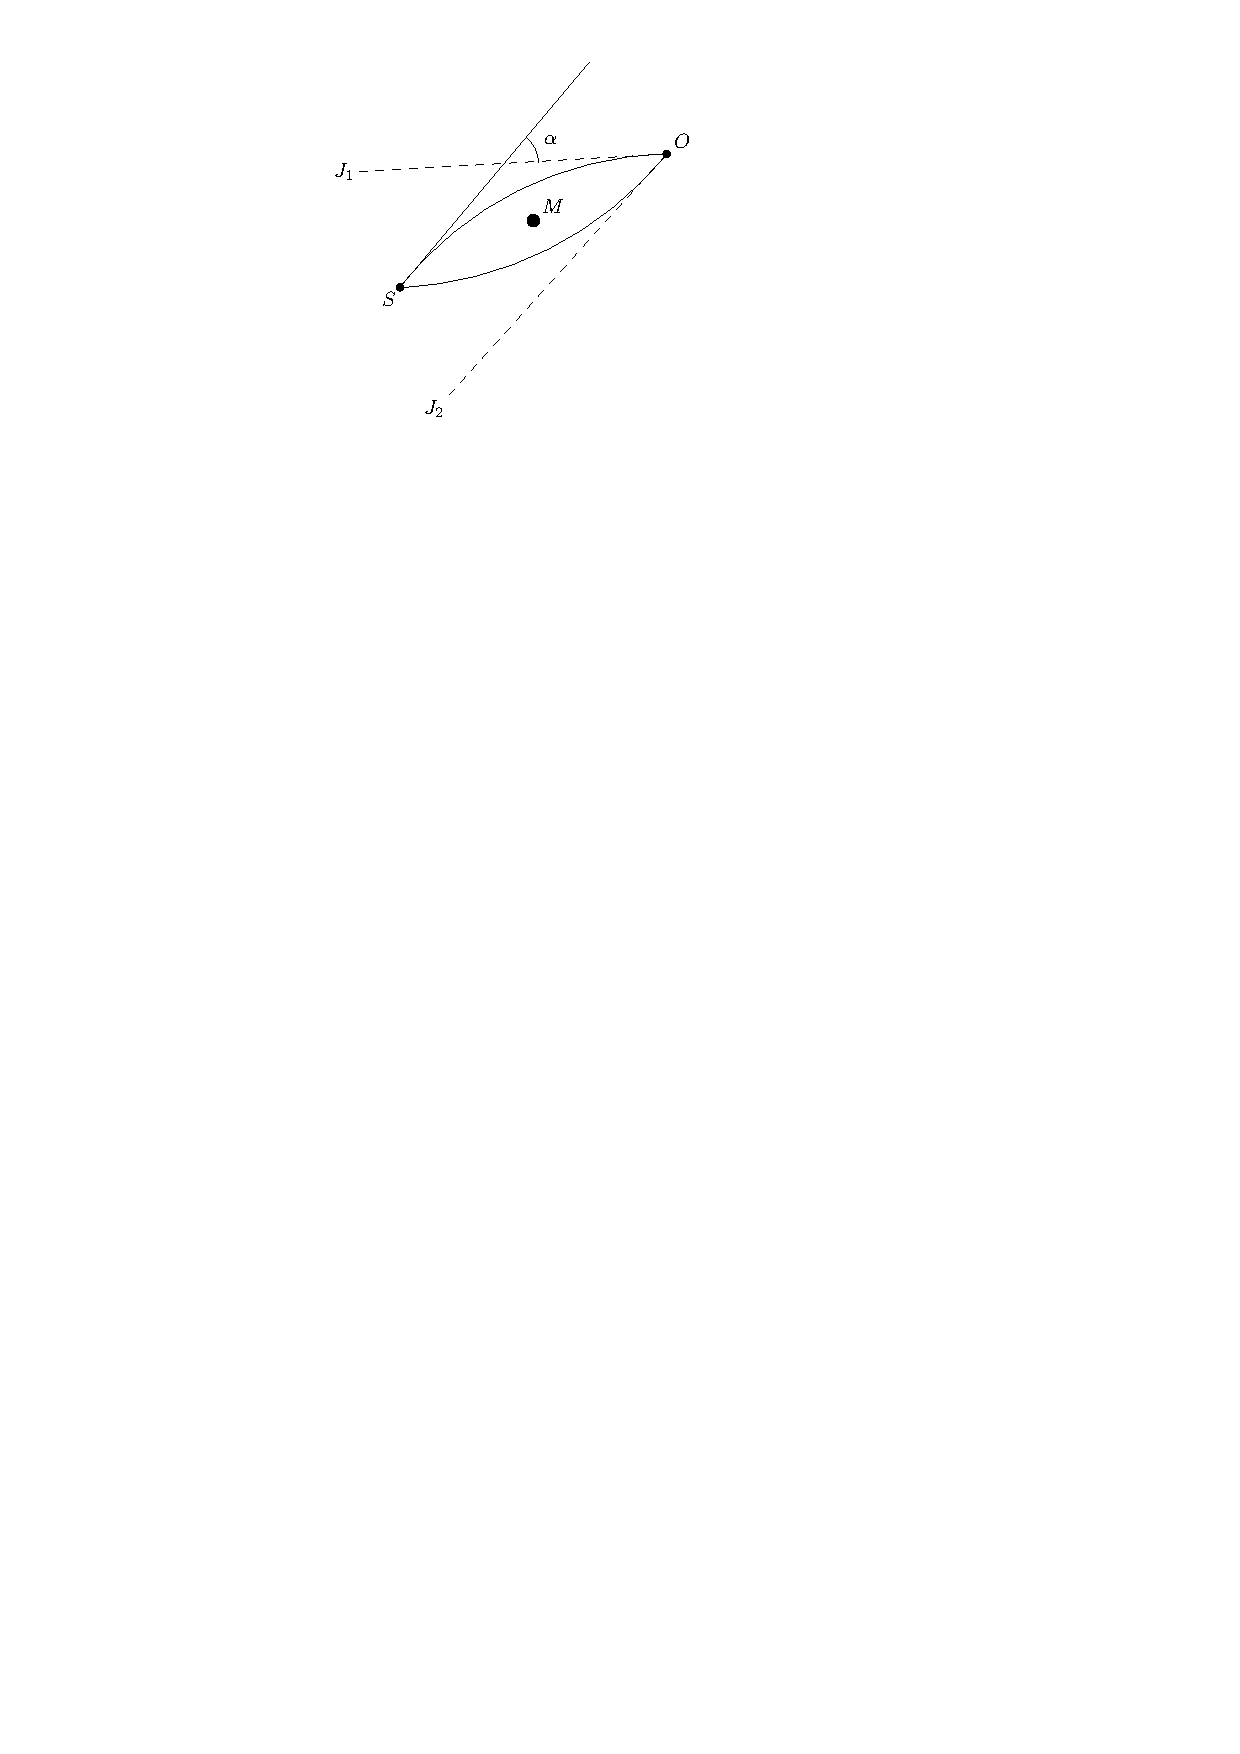
\includegraphics[width=0.4\textwidth]{grav-lens}
\caption{Гравитационное линзирование}\label{grav-lens}
\end{center}
\end{figure}

Найти угол отклонения луча в радианах можно по следующей формуле:
\begin{equation}
\alpha=\frac{4GM}{Rc^2},
\end{equation}
где $M$ --- масса тела, отклоняющего луч, $R$ --- радиус этого тела, $c$ --- скорость света.
% todo: нужно проверить, что все доехало
%\subsection{Закон Хаббла}
\term{Закон Хаббла}~--- эмпирический закон, связывающий скорость удаления галактик $V$ и расстояние $R$ до них линейным образом:
\begin{equation}
	V = H R,
\end{equation}
величина $H=68~\text{км/c} \cdot \text{Мпк}$ называется \imp{постоянной Хаббла}.

При $v \ll c$ можно использовать приближение эффекта Доплера, тогда
\begin{equation}
	V = c z.
	\label{eq:hubble-speed}
\end{equation}

Равенство \eqref{eq:hubble-speed} справедливо только при $z \ll 1$, а при б\'{o}льших значениях $z$ космологическое красное смещение нельзя связывать с эффектом Доплера, поэтому можно пользоваться только формулой
\begin{equation}
	\frac{dz}{dt} = - H(z)(1+z),
\end{equation}
где постоянная Хаббла введена как функция красного смещения.
 % переехало в Космологию 
\subsection{Шкала электромагнитных волн}

\term{Гамма излучение} возникает при радиоактивных распадах ядер, при торможении электронов энергией более $10^5$~эВ и при других взаимодействиях элементарных частиц. Используются в гамма-дефектоскопии, при изучении свойств вещества.

\term{Рентгеновские лучи} излучаются при большом ускорении электронов, например при их торможении в металлах. Получают их при помощи рентгеновской трубки: электроны в вакуумной трубке ускоряются электрическим полем при высоком напряжении, достигая анода, при со­ударении резко тормозятся. При торможении электроны движут­ся с ускорением и излучают электромагнитные волны с малой длиной.

\begin{figure}[!h]
	\centering
	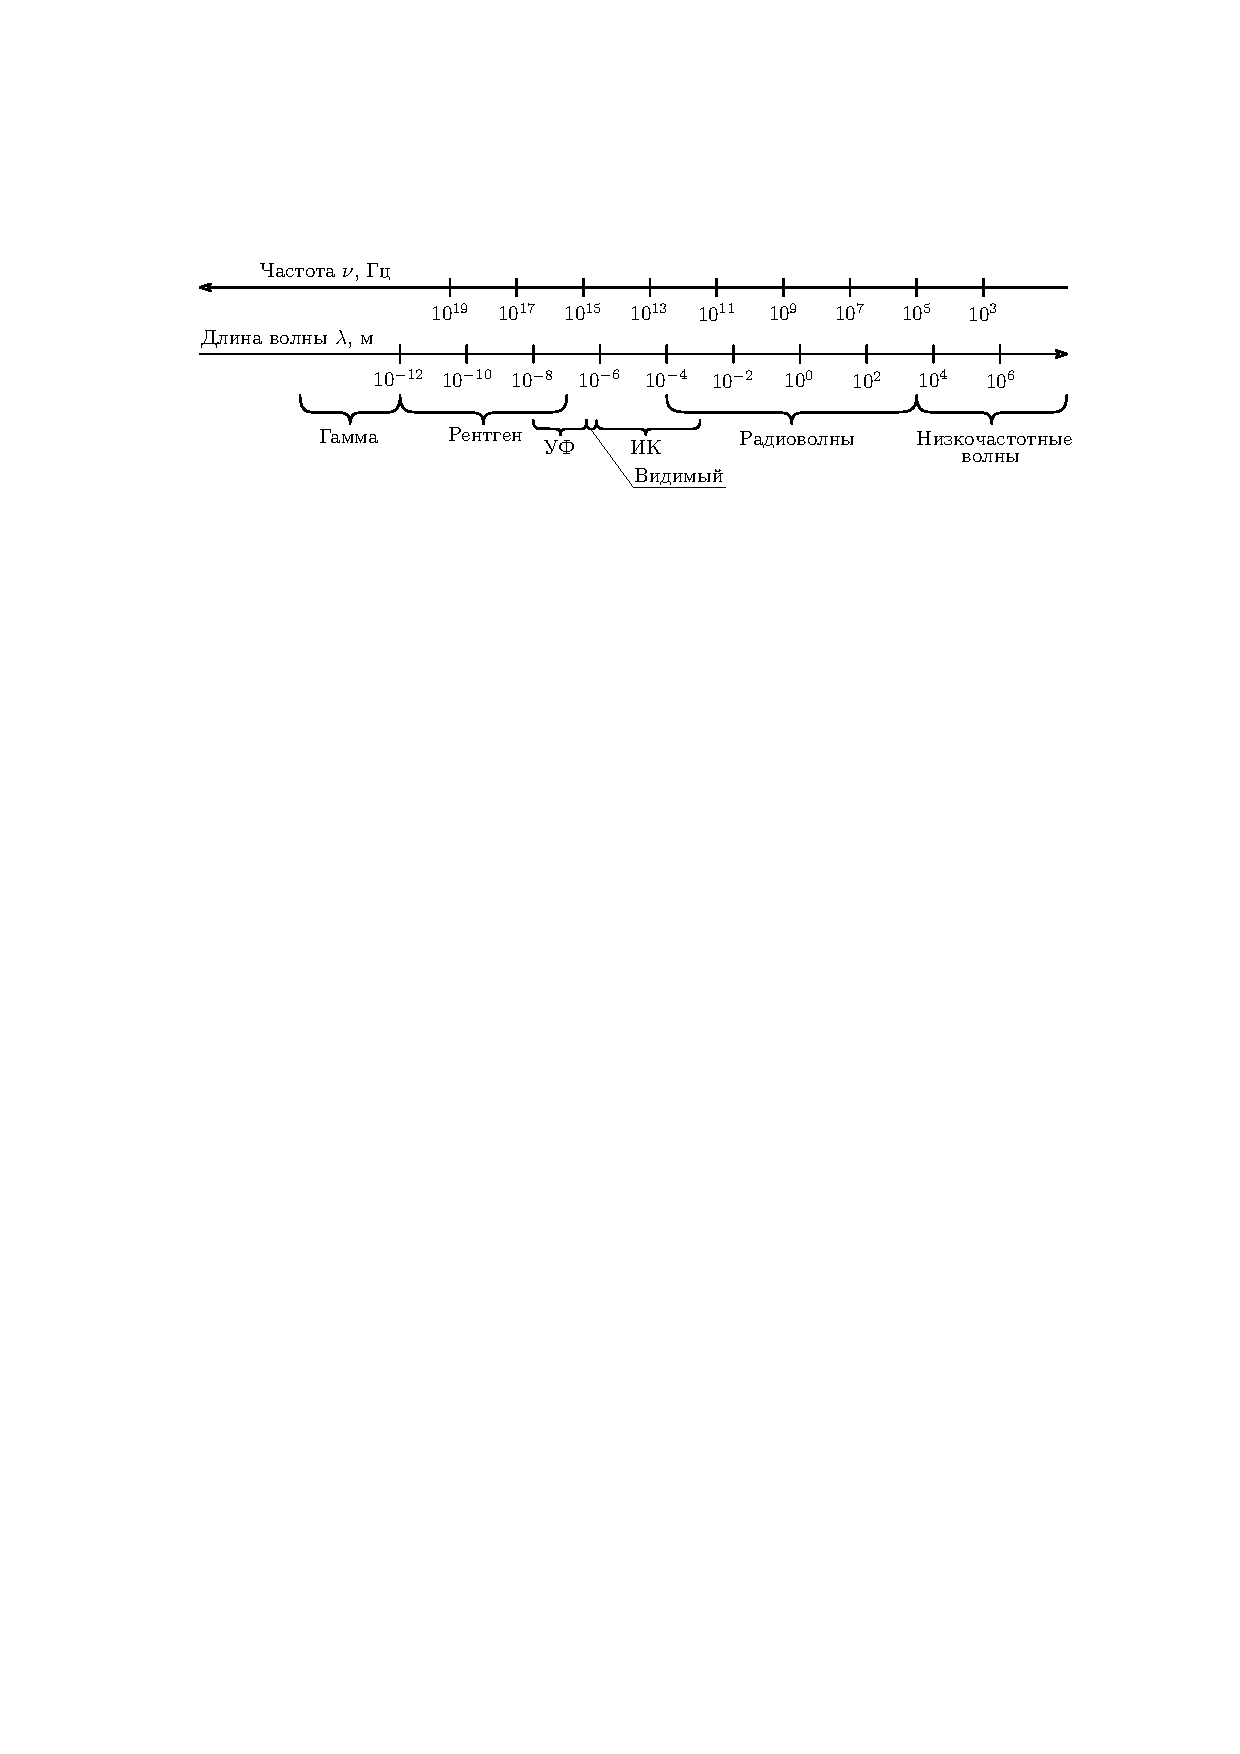
\includegraphics[width = 1\textwidth]{scale-wave.pdf}
	\caption{Шкала электромагнитных волн}
\end{figure}
\term{Ультрафиолетовые лучи}~--- излучение Солнца, ртутных ламп и т.\,п. Используются в ультрафиолетовой микроскопии, в медицине.

\term{Видимое излучение}~--- часть электромагнитного излучения, воспринимаемая глазом (от фиолетового до от красного).

\term{Инфракрасное излучение}~--- тепловое, излучается любым нагретым телом.

\term{Радиоволны} используются повсеместно в обычной жизни, это и сотовая связь, и радиолокация, и спутниковая связь, и Wi-Fi и многое другое.

\term{Низкочастотные волны}~--- диапазон, традиционно используемый в электротехнике. В промышленной электроэнергетике используется частота 50~Гц, на~которой осуществляется передача электрической энергии по линиям и преобразование напряжений трансформаторными устройствами.

\subsection{Специальная теория относительности. Аберрация}

Обычно в СТО рассматриваются две инерциальные системы $S$ и $S'$. Время и координаты некоторого события, измеренные относительно системы $S$, обозначаются как $(t, x, y, z)$, а координаты и время этого же события, измеренные относительно системы $S'$, как $(t', x', y', z')$. Удобно считать, что координатные оси систем параллельны друг другу, и система $S'$ движется вдоль оси $x$ системы $S$ со скоростью $v$. Одной из задач СТО является поиск соотношений, связывающих $(t', x', y', z')$ и $(t, x, y, z)$, которые называются \textit{преобразованиями Лоренца}. Общий вид \term{преобразований Лоренца} в векторном виде, когда относительная скорость систем отсчёта имеет произвольное направление:
\begin{equation}
    t'=\gamma\cdot \left(t-\frac{(\vec{r},\vec{v})}{c^2}\right),
\end{equation}
\begin{equation}
    \vec{r'} = \vec{r} - \gamma \vec{v} t + (\gamma - 1) \cdot \frac{(\vec{r},\vec{v})\vec{v}}{v^2},
\end{equation}
где  $\gamma = \dfrac{1}{\sqrt{1 - \frac{v^2}{c^2}}} \equiv \dfrac{1}{\sqrt{1-\beta^2}}$~--- Лоренц фактор, являющийся коэффициентом масштабирования; $\vec{r}$ и $\vec{r'}$ --- радиус-векторы события относительно систем отсчёта $S$ и $S'$.

Если сориентировать координатные оси по направлению относительного движения инерциальных систем и выбрать это направление в качестве оси $x$, то преобразования Лоренца примут вид:
\begin{equation}
    t'=\gamma \left(t - \frac{v x}{c^2} \right),\quad\quad x'= \gamma \left( x-vt \right), \quad\quad y'=y,\quad\quad z'=z.
\end{equation}

При скоростях много меньше скорости света $(v\ll c)$ преобразования Лоренца переходят в \textit{преобразования Галилея}:
\begin{equation}
    t'=t,\quad\quad x'=x-vt,\quad\quad  y'=y,\quad\quad  z'=z.
\end{equation}

\term{Аберрация} --- явление, состоящее в том, что движущийся наблюдатель видит светило не в том направлении, в котором он видел бы его в тот же момент, если бы находился в покое. Причём светило  смещается в сторону движения наблюдателя. Это происходит из-за конечности скорости света и из-за изменения системы отсчёта для наблюдателя.
Угол аберрационного смещения можно найти по следующей формуле
\begin{equation}\sigma=\frac{v}{c}\sin\theta,
\end{equation}
где $v$ --- скорость наблюдателя, $\theta$ --- угол между направлением вектора скорости наблюдателя и направлением на объект.

\subsection{Оптическая толщина. Закон Бугера -- Ламберта -- Бера}
\begin{wrapfigure}[10]{c}{0.4\tw}
	\centering
	\begin{tikzpicture}
		\footnotesize
		
		\foreach \x in {-1, -.9, ..., 1.01} {
		\foreach \y in {-1.5, -1.4, ..., 1.51} {
		\pgfmathsetmacro\radius{(rand+1)/60};
		\fill [lightgray] (\x + rand*.03, \y + rand*.03)  circle(\radius);
		};
		};
		
		\draw [line width=1pt](-2, 0) -- (-1, 0);
		\draw [line width=1pt, -latex](-2, 0) -- (-1.4, 0);
		\fill[left color=black, right color=lightgray] (-1, -.5pt) rectangle (1, .5pt);
		\draw [line width=1pt, lightgray](1, 0) -- (2, 0);
		\draw [line width=1pt, lightgray, -latex](1, 0) -- (1.6, 0);
		
		\draw (-1.5, .1) node[anchor=south] {$I_0$};
		\draw (1.5, .1) node[anchor=south] {$I$};
		
		\draw [latex-latex] (-1.05, -1.7) -- (1.05, -1.7);
		\draw (0, -1.7) node[anchor=north] {$L$};
	\end{tikzpicture}
	\caption{}
	\label{}
\end{wrapfigure}
Рассмотрим процесс прохождение электромагнитного излучения с интенсивностью $I_0$ через слой толщины $L$ непрозрачных частиц со средней концентрацией $n$ и сечением поглощения $\sigma$. Ясно, что интенсивность выходящего из слоя пыли излучения будет меньше начальной. Выясним, по какому закону падает интенсивность излучения в таком случае.

Для этого рассмотрим тонкий слой толщины $dx$ из всего слоя частиц. Пусть на входе в этот тонкий слой излучение имеет интенсивность $I$, а на выходе из слоя~--- $I - dI$. Часть излучения прошла сквозь тонкий слой, а часть поглотилась пылинками, общая площадь которых равна произведению их количества в этом слое на среднюю площадь поглощения. Здесь можно считать, что перекрытия частиц друг другом не происходит, так как рассматриваемый слой достаточно тонкий. Количество частиц  $dN$ в тонком слое зависит только от их концентрации и площади всего слоя, таким образом:
\begin{equation*}
	N = n S \, dx.
\end{equation*}
Тогда можно составить уравнение на изменение интенсивности излучения тонким слоем:
\begin{equation*}
	-\frac{dI}{I} = \frac{N\sigma}{S} = n\sigma \, dx.
\end{equation*}
Проинтегрируем левую и правую часть полученного уравнения:
\begin{gather*}
	-\int\limits_{I_0}^{I} \frac{dI}{I} = \int\limits_{0}^{L} n \sigma \, dx,\\
	-\ln I + \ln I_0 = n\sigma L,\\[.5pc]
	%	e^{-\ln I_0} \cdot e^{\ln I} = e^{n \sigma L},
	I = I_0 e^{-n\sigma L}. \tag{\theequation}
\end{gather*}

\term{Оптическая толщина}~--- безразмерная величина, характеризующая степень непрозрачности среды для проходящего сквозь неё излучения. В общем случае, конечно, концентрация частиц и их площадь сечения взаимодействия могут меняться от координаты, поэтому оптическая толщина определяется как
\begin{equation}
	\tau = \int n(x) \sigma(x)\,dx.
\end{equation}
Для случая постоянных $n$ и $\sigma$, как было получено выше, $\tau = n \sigma L$.

Связь интенсивности $I_0$ на входе с интенсивностью $I$ на выходе называется \term{Законом Бугера -- Ламберта -- Бера} и записывается в виде
\begin{equation}
	I = I_0 e^{-\tau}.
\end{equation}

Определим теперь среднюю длину пути $\langle l \rangle$ луча в слое до момента поглощения частицей. Будем в этом случае считать, что $L = \infty$. Вероятность поглощения луча слоем толщины $dx$ в приближении постоянной концентрации и площади эффективного сечения равна
\begin{equation*}
	p(x) = \frac{-dI(x) / dx}{I_0} = n \sigma e^{-n\sigma x}
\end{equation*}

Тогда средняя длина пути определяется как
\begin{multline*}
	\langle l \rangle 
	= \int\limits_0^\infty x p(x) \, dx 
	= \int\limits_0^\infty x n \sigma e^{-n\sigma x} \, dx =\\
	= - x e^{-n \sigma x}\big|_{0}^{\infty} -  \int\limits_0^\infty e^{-n\sigma x} \, dx 
	= 0 + \frac{1}{n \sigma} \cdot e^{-n \sigma x} \big|_0^\infty = \frac{1}{n \sigma}.
\end{multline*}
Величина $\langle l \rangle$ называется \imp{средней длиной свободного пробега} или просто \term{длиной свободного пробега}.


\subsection{Фотометрия. Показатель цвета}
\term{Фотометрическая система UBV}~--- система, разработанная для классификации звезд в зависимости от их цвета. В этой системе измеряются звездные величины звезд на трех участках спектра: $U$ (максимум чувствительности $\lambda_\text{макс}^U = 350$~нм), $B$ ($\lambda_\text{макс}^B = 430$~нм) и $V$ ($\lambda_\text{макс}^V = 550$~нм). Для звёзд спектрального класса A0V все три значения равны, поэтому такие звёзды являются фотометрическим стандартом. Одним из таких стандартов является яркая звезда северного неба Вега.

\term{Показатель цвета} $(B-V)$~--- разница блеска объекта в фильтрах $B$ и $V$, измеряется в звёздных величинах. Существует эмпирическая зависимость, связывающая показатель цвета $(B-V)$ и температуру  объекта,
\begin{equation}
	T = 4600 \cdot\left(\frac{1}{0.92\left(B-V\right) + 1.7} + \frac{1}{0.92\left(B-V\right) + 0.62}\right).
\end{equation}

\term{Избыток цвета} $E\left(B - V\right)$~--- разность между наблюдаемым показателем цвета звезды и нормальным, свойственным ее спектральному классу.
\begin{equation}
	E\left(B - V\right) = \left(B - V\right) - \left(B - V\right)_0 = \left(B - B_0\right) - \left(V - V_0\right) = A_B - A_V,
\end{equation}
величины $A_B$ и $A_V$~--- поглощения на голубом и видимом участках спектра.

\term{Межзвёздное поглощение}~--- суммарный эффект рассеяния и истинного поглощения света пылевыми частицами в межзвёздной среде. Известно соотношение, связывающее межзвёздное поглощение с избытком цвета,
\begin{equation}
	\frac{A_V}{E\left(B - V\right)} = R \approx 3.1.
\end{equation}

%Поглощение света в среде зависит от длины волны, и установлена эмпирическая зависимость
%\begin{equation}
%A_B - A_V = 1.086 \bigl(\tau\left(B\right) - \tau\left(V\right)\bigr),
%\end{equation}
%где $\tau\left(B\right)$ и $\tau\left(V\right)$~---  оптические толщины в голубом и видимом диапазоне.

\subsection{МКТ и термодинамика}
\term{Молекулярно-кинетическая теория} изучает процессы, происходящие в макроскопических телах, на основе предположения о том, что вещество состоит из частиц, движение которых подчиняется законам механики Ньютона.

\term{Уравнение Менделеева-Клайперона} является следствием этой теории и~связывает давление $(P)$, объем $(V)$ и температуру $(T)$ идеального газа:
\begin{equation}
    PV = \nu R T,
    \label{eq:mkt-idial-gas}
\end{equation}
здесь $R = 8.31~\text{м}^2 \cdot \text{кг} \cdot \text{с}^{-2} \cdot \text{К}^{-1} \cdot \text{моль}^{-1}$~--- \imp{универсальная газовая постоянная}, а $\nu$~--- количество вещества идеального газа. Иначе, можно записать
\begin{equation}
    P = nkT =  \frac{\rho}{\mu}RT,
    \label{eq:mkt-p}
\end{equation}
где $n$~--- концентрация, $k$~--- постоянная Больцмана, $\rho$~--- плотность газа, $\mu$~--- молярная масса.

Частицы газа имеют равномерное распределение в предоставленном пространстве и распределение Максвелла по энергиям, то есть вероятность, что частица обладает энергией $E$ равна
\begin{equation}
    f_E(E) = \frac {2\pi \sqrt{E}}{\sqrt{(\pi kT)^3}}  \exp\left(\frac {-E} {kT} \right).
    \label{eq:maxwell}
\end{equation}
После некоторых математических преобразований несложно получить выражение для средней энергии $\langle E \rangle$ частиц идеального газа:
\begin{equation}
    \langle E \rangle = \frac{3}{2}kT,
\end{equation}
следовательно, \term{среднеквадратичная скорость} определяется, как
\begin{equation}
    \langle v^2 \rangle = \frac{3kT}{m}.
\end{equation}
Однако, исходя из распределения \eqref{eq:maxwell}, \imp{наиболее вероятная скорость} частиц
\begin{equation}
    v_\text{н.в.} = \sqrt{\frac{2kT}{m}}.
\end{equation}

\term{Первое начало термодинамики} гласит:
\begin{equation}
    \delta Q = dU + \delta A,
\end{equation}
где $\delta Q$~--- подведенная теплота, $d U$~--- изменение внутренней энергии газа, $\delta A$~--- работа газа.

\imp{Внутренняя энергия} газа определяется соотношением
\begin{equation}
    U = \frac{i}{2}RT,
\end{equation}
здесь $i$~--- количество степеней свободы частиц газа.

\term{Теплоёмкость идеального газа}~--- отношение количества сообщённой газу теплоты $\Delta Q$, к произошедшему изменению температуры $\Delta T$, в расчёте на один моль:
\begin{equation}
    C = \frac{\delta Q}{dT}
\end{equation}

\term[изотермический процесс]{Изотермический} процесс~--- при котором температура газа не изменяется:
\begin{equation}
    PV = \const, \quad\quad C_T = +\infty,
\end{equation}
индекс теплоёмкости соответствует величине, постоянной в течение процесса.

\term[изохорический процесс]{Изохорический} процесс~--- когда объём, занимаемый газом, не изменяется:
\begin{equation}
    \frac{P}{T} = \const, \quad\quad C_V = \frac{i}{2}R.
\end{equation}

\term[изобарический процесс]{Изобарический} процесс~--- тот, при котором давление газа не изменяется:
\begin{equation}
    \frac{V}{T} = \const, \quad\quad C_P = \frac{i+2}{2}R = C_V + R.
\end{equation}

\term[адиабатический процесс]{Адиабатический} процесс~--- процесс, в котором количество подведенной теплоты $\delta Q$ равно нулю:
\begin{equation}
    P V^\alpha = \const, \quad\quad C_Q = 0,
\end{equation}
где $\alpha = C_P/C_V$~--- показатель адиабаты.

\subsection{Атмосфера Земли}
Применим знания о МКТ для поиска характерной высоты атмосферы Земли в двух её моделях: изотермической и адиабатической атмосферах. Прежде, чем приступим к поиску, несколько фактов об атмосфере Земли. Давление у поверхности Земли в среднем составляет 
\begin{equation*}
	p_0 = 1~\text{атм} = 101325~\text{Па} = 760~\text{мм рт. ст}.
\end{equation*}
Наблюдаемые отклонения от среднего значения незначительны для последующих выкладок, так как составляют не более $5\%$. 

Средняя температура воздуха у поверхности $T_0 \approx 12^\circ\text{C} = 285~\text{K}$. Молярная масса воздуха, средневзвешенное молярных масс его компонент, $\mu_0 = 29~\text{г}/\text{моль}$. 

\paragraph{Изотермическая атмосфера} Падение давления воздуха с увеличением высоты можно описать математически~\cite{barometric-formula-isotermal}. Для этого рассмотрим тонкий слой воздуха толщиной $dh$, выделим в нём фрагмент с площадью $dS$. Пусть масса воздуха в этом фрагменте равна $dm$.  Представим, что воздух в выделенном фрагменте окружен невесомой тонкой оболочкой~--- не перемешивается с окружающим воздухом и находится в равновесии. Которое достигается благодаря равенству нулю равдействующей трёх сил: силы давления воздуха снизу $F_\uparrow = p\d S$, силы давления воздуха сверху $F_\downarrow = -(p + dp)\d S$ и силы тяжести $F_g = -g\d m$, действующей на выделенный слой. Здесь $dp < 0$, так как с высотой давления, очевидно, уменьшается, потому что все меньший столб воздуха оказывает давление на рассматриваемый слой. Итак,
\begin{gather}
	F_\uparrow + F_\downarrow + F_g = 0,\nonumber\\
	p \d S - (p + dp) \d S - g \d m = 0,\nonumber\\
	- dp\d S = g \rho \d V = g \rho \d h \d S,\nonumber\\
	dp = - g \rho \d h. \label{eq:isotherm-atm-dp}
\end{gather}

Из уравнения состояния идеального газа \eqref{eq:mkt-p}, считая воздух таковым, выразим плотность воздуха $\rho$:
\begin{equation*}
	\rho = \frac{p \mu}{RT}.
\end{equation*}
Подставив полученное выражение в~\eqref{eq:isotherm-atm-dp}, получим,
\begin{equation}
	dp = - \frac{\mu g}{RT} p \d h.
	\label{eq:earth-atm-dp}
\end{equation}

Разделим переменные и проинтегрируем левую и правую часть от нуля до высоты $h$:
\begin{gather}
	\int\limits_{p_0}^{p(h)} \frac{dp}{p} = -\int\limits_0^h \frac{\mu g}{RT} dh,\nonumber\\
	\ln p(h) - \ln p_0 = -\frac{\mu g h}{RT},\nonumber\\
	p(h) = p_0 \exp \left[ -\frac{\mu g h}{RT} \right]. \label{eq:earth-atm-isot}
\end{gather}
Полученное равенство называется \imp{барометрической формулой для изотермической атмосферы}. Из нее следует, что характерная (давление уменьшилось в $e$ раз) высота изотермической атмосферы
\begin{equation*}
	H_{T=\const} = \frac{RT}{\mu g} \simeq 8~\text{км}.
\end{equation*}

\paragraph{Адиабатическая атмосфера}
Конечно, предположение об изотермичности атмосферы достаточно грубо. Рассмотрим модель, в рамках которой выполняется равенство $dQ = 0$ для выделенного тонкого слоя воздуха~--- адиабатическую модель атмосферы~\cite{barometric-formula-adiabatic}.

Такая модель хорошо описывает наблюдаемые в атмосфере процессы. Наибольший нагрев воздуха происходит у поверхности Земли, и чем выше, тем воздух холоднее. Это хорошо заметно в горах, где воздух холоднее, чем в нижележащих долинах. В ходе конвекции слои теплого воздуха поднимаются и расширяются, так как давление окружающего воздуха с высотой уменьшается. Работа газа по его расширению уменьшает его внутреннюю энергии~--- газ остывает.

Приступим к выводу барометрической формулы для адиабатической атмосферы. Начнем с выражений для работы газа и изменения его потенциальной энергии:
\begin{gather*}
	\delta A = p \d V,\\
	dU = C_V \nu \d T.
\end{gather*}
Запишем первое начало термодинамики для тонкого слоя воздуха:
\begin{gather}
	dQ = 0 = dU + \delta A = p \d V + C_V \nu \d T,\notag\\
	dT = - \frac{p}{C_V \nu} dV.
	\label{eq:earth-atm-dt}
\end{gather}
Выразим объем из уравнения состояния идеального газа \eqref{eq:mkt-idial-gas} и перейдем к дифференциалам:
\begin{equation}
	dV = d \left(\frac{\nu R T}{p} \right) = \frac{\nu R}{p} \d T - \frac{\nu R T}{p^2} \d p.
	\label{eq:earth-atm-dv}
\end{equation}
Подставив \eqref{eq:earth-atm-dv} в уравнение \eqref{eq:earth-atm-dt}, получим
\begin{gather*}
	dT = - \frac{p}{C_V \nu} \left( \frac{\nu R}{p} \d T - \frac{\nu R T}{p^2} \d p \right),\\
%	\left( 1 + \frac{R}{C_V} \right)\frac{dT}{T} = \frac{R}{C_V} \frac{dp}{p},\\
	\therefore \frac{dT}{T} = \frac{R}{C_V + R} \frac{dp}{p} = \frac{R}{C_p} \frac{dp}{p}.
\end{gather*}
Воспользуемся выражением~\eqref{eq:earth-atm-dp} для $dp$:
\begin{gather}
	\frac{d T}{T} = -\frac{\mu g}{C_P T} \d h,\\
	\frac{dT}{dh} =  -\frac{\mu g}{C_P} \equiv \Gamma.\label{eq:ad-therm-grad}
\end{gather}

Выражение~\eqref{eq:ad-therm-grad} показывает, что в случае адиабатической атмосферы градиент температуры $\Gamma$ является постоянной величиной. Поэтому справедливо, температура воздуха $T(h) = T_0 + \Gamma h$, где $T_0$~--- температура у поверхности. Молярная теплоёмкость воздуха при постоянном давлении $C_p = 29.15$~Дж/моль, поэтому градиент температуры~$\Gamma$ составляет~$-0.83$~К на 100~м. 

Вернемся к уравнению \eqref{eq:earth-atm-dp} и подставим в него полученное выражение для температуры, чтобы получить барометрическую формулу:
\begin{gather*}
	dp = - \frac{p \mu g}{RT(h)} dh,\\
	\int\limits_{p_0}^{p(H)} \frac{dp}{p} = - \frac{\mu g}{R} \int\limits_0^H \frac{dh}{T_0 + \Gamma h}= - \frac{\mu g}{R\Gamma} \int\limits_0^H \frac{d(T_0 + \Gamma h)}{T_0 + \Gamma h},\\
	\ln \frac{p(H)}{p_0} = - \frac{\mu g}{R\Gamma} \ln \frac{T_0 + \Gamma H}{T_0},\\
	p(H) = p_0 \left(1 + \frac{\Gamma H}{T_0} \right)^{ - \mu g /R\Gamma} =  p_0 \left(1 + \frac{\Gamma H}{T_0} \right)^{ - C_p/R}.
\end{gather*}

Отсюда получаем, что высота характерная высота адиабатической атмосферы
\begin{equation*}
	H_{dQ=0} = \left(\exp \left[ \frac{R}{C_p} \right] - 1 \right) \cdot  \frac{T_0}{\Gamma} = 9.6~\text{км}.
\end{equation*}

\begin{figure}[h]
	\centering
	\begin{tikzpicture}
	\begin{axis}[
		height	=	6cm,
		width	=	8cm,
		xlabel	=	{$H$, км},
		ylabel	=	{$p(H)$, км},
%		ylabel shift	= -1 cm,
		ymax=1,
		ymin=0,
		xmin=0,
		xmax=10,
		legend cell align=left,
			legend style={
			draw=none,
			fill=none,
			font=\scriptsize,
			at={(axis cs:1, 0.1)}, anchor=south west,
			row sep=.5pc,
			},
		]
		
		\addplot[smooth, domain=0:10, samples=200] {1 * exp(-0.029*9.81*x*1000/8.31/285) };
		\addplot[smooth, domain=0:10, samples=200, gray] {1 * (1 + 10*x/285)^(-0.029*9.81/8.31/0.00975)};
		\legend{
			$T=\const$,
			$dQ = 0$
		};
	\end{axis}
\end{tikzpicture}
\end{figure}



















\subsection{Атмосферные эффекты}

\subsubsection{Радуга}
\def\drawRainbow(#1){% (count)
    \tkzInit[xmin=-0.4, ymin=-1.5, xmax=2.1, ymax=1.1]
    \tkzClip
    
    \tkzDefPoint(0,0){R}
    \tkzDefPoint(1,0){C}
    
    \foreach \x in {-0.02,-0.04,...,-1} {
        \tkzSetUpLine[gray]

        \tkzDefPoint(-0.5,\x){A}
        \tkzDefPoint(0,\x){B}
        
        \tkzInterLC(B,A)(C,R) 
        \tkzGetPoints{R1}{x}
        
        \tkzDrawSegment(A,R1)
        
        \tkzFindAngle(A,R1,C) 
        \tkzGetAngle{ABC}
        
        \pgfmathparse{\ABC - 180}
        \pgfmathsetmacro\ALPHA{\pgfmathresult}
        
        \pgfmathparse{asin(sin(\ALPHA)/1.333)}
        \pgfmathsetmacro\BETA{\pgfmathresult}
        
        \tkzDefPointBy[homothety=center R1 ratio 1](R1) 
        \tkzGetPoint{R2}
        \foreach \i in {0,1,...,#1} {
            \tkzDefPointBy[rotation=center R1 angle -\BETA](C) 
            \tkzGetPoint{R1'}
            
            \tkzInterLC(R1,R1')(C,R) 
            \tkzGetPoints{x}{R2}
            
            \tkzDrawSegment(R1,R2)
            
            \tkzDefPointBy[homothety=center R1 ratio 1](R2) 
            \tkzGetPoint{R1}
        }
        
        \tkzDefPointBy[rotation=center R1 angle -180 + \ALPHA](C) 
        \tkzGetPoint{L'}
        
        \tkzDefPointBy[homothety=center R1 ratio 1.5](L') 
        \tkzGetPoint{L}
        
        \tkzDrawSegment(R2,L)
    }
        
    \tkzDefPoint(-0.5,0){A0}
    \tkzDefPoint(2,0){B0}
    \tkzDrawSegment[dotted, thick](A0,B0))
        
    \tkzDrawCircle[thick, black](C,R)
}
\def\drawRainbowDispersion(#1){% (count)
    \tkzInit[xmin=-0.4, ymin=-1.5, xmax=2.1, ymax=1.1]
    \tkzClip
    
    \tkzDefPoint(0,0){R}
    \tkzDefPoint(1,0){C}
    
    \foreach \n in {1.332,1.334,...,1.345} {
        \tkzSetUpLine[gray]

        \pgfmathparse{sqrt((1 + #1)^2 -\n^2)/sqrt(2 * #1 + #1 * #1)}
        \pgfmathsetmacro\x{\pgfmathresult}

    
        \tkzDefPoint(-0.5,-\x){A}
        \tkzDefPoint(0,-\x){B}
        
        \tkzInterLC(B,A)(C,R) 
        \tkzGetPoints{R1}{x}
        
        \tkzDrawSegment(A,R1)
        
        \tkzFindAngle(A,R1,C) 
        \tkzGetAngle{abc}
        
        \pgfmathparse{\abc - 180}
        \pgfmathsetmacro\ALPHA{\pgfmathresult}
            
        \pgfmathparse{asin(sin(\ALPHA)/\n)}
        \pgfmathsetmacro\BETA{\pgfmathresult}
        
        \tkzDefPointBy[homothety=center R1 ratio 1](R1)
        \tkzGetPoint{R2}
        
        \foreach \i in {0,1,...,#1} {
            \tkzDefPointBy[rotation=center R1 angle -\BETA](C) 
            \tkzGetPoint{R1'}
            
            \tkzInterLC(R1,R1')(C,R) 
            \tkzGetPoints{x}{R2}
            
            \tkzDrawSegment(R1,R2)
            
            \tkzDefPointBy[homothety=center R1 ratio 1](R2) 
            \tkzGetPoint{R1}
        }
                
        \pgfmathparse{-180+\ALPHA}
        \pgfmathsetmacro\r{\pgfmathresult}
        
        \tkzDefPointBy[rotation=center R1 angle \r](C) 
        \tkzGetPoint{L'}
        
        \tkzDefPointBy[homothety=center R1 ratio 1](L') 
        \tkzGetPoint{L}
        
        \tkzDrawSegment(R1,L)
    }
        
    \tkzDefPoint(-0.5,0){A0}
    \tkzDefPoint(2,0){B0}
    \tkzDrawSegment[dotted, thick](A0,B0))
        
    \tkzDrawCircle[thick, black](C,R)
}
\begin{figure}
    \begin{subfigure}{0.32\tw}
        \begin{tikzpicture}[scale=1.3]
            \begin{scope}[yscale=-1]
                \drawRainbow(1)
            \end{scope}
        \end{tikzpicture}
        \captionof{figure}{}
    \end{subfigure}
    \hfill
    \begin{subfigure}{0.32\tw}
        \begin{tikzpicture}[scale=1.3]
            \drawRainbow(2)
        \end{tikzpicture}
        \captionof{figure}{}
    \end{subfigure}
    \hfill
    \begin{subfigure}{0.32\tw}
        \begin{tikzpicture}[scale=1.3]
            \drawRainbow(3)
        \end{tikzpicture}
        \captionof{figure}{}
    \end{subfigure}
    \\
    \begin{subfigure}{0.32\tw}
        \begin{tikzpicture}[scale=1.3]
            \begin{scope}[yscale=-1]
                \drawRainbowDispersion(1)
            \end{scope}
            \tkzDefPoint(1.2,-1.15){Label}
            \tkzLabelPoint[below](Label){\tiny$42.2^\circ$}
            \tkzLabelPoint[left=4pt](Label){\tiny$40.5^\circ$}
        \end{tikzpicture}
        \captionof{figure}{}
    \end{subfigure}
    \hfill
    \begin{subfigure}{0.32\tw}
        \begin{tikzpicture}[scale=1.3]
            \drawRainbowDispersion(2)
            \tkzDefPoint(-0.2,-0.3){Label}
            \tkzLabelPoint[below](Label){\tiny$53.7^\circ$}
            \tkzLabelPoint[left=3pt](Label){\tiny$50.6^\circ$}
        \end{tikzpicture}
        \captionof{figure}{}
    \end{subfigure}
    \hfill
    \begin{subfigure}{0.32\tw}
        \begin{tikzpicture}[scale=1.3]
            \drawRainbowDispersion(3)
            \tkzDefPoint(1.1,-1.3){Label}
            \tkzLabelPoint[right=2pt](Label){\tiny${51.9^\circ}$}
            \tkzLabelPoint[left=2pt](Label){\tiny${55.1^\circ}$}
        \end{tikzpicture}
        \captionof{figure}{}
    \end{subfigure}
    \caption{}
    \label{}
\end{figure}
\subsection{Давление и температура в центре звезды}
В данном разделе найдем оценку для давления и температуры в центре звезды. Для этого рассмотрим такую модель, пусть звезда~--- однородное газовое облако радиусом $R$. Пусть плотность звезды равна $\rho$, а вещество~--- водородоподобная плазма, такое допущение справедливо для звёзд на главной последовательности. Тогда средняя масса частиц газа составляется примерно $m = 0.5m_p$, потому вещество состоит из одинакового числа протонов и электронов, так как в целом оно нейтрально, а $m_e \ll m_p$.

Аналогично поиску высоты атмосферы рассмотрим тонкий слой вещества высоты $dr$ с площадью сечения $dS$ на расстоянии $r$ от центра звезды. Пусть его масса  равна $dm$. На слой действуют три силы: сила давления газа снизу $F_\uparrow = p(r)\,d S$, сила давления газа сверху $F_\downarrow = -p(r + \,d r)\,d S$ и сила гравитационного притяжения $F_g = -GM(r)/r^2\,d m$ от массы, находящейся внутри сферы радиуса $r$, так как суммарное воздействие от внешней оболочка равно нулю. Стационарность звезды обеспечивается балансом этих сил, значит
\begin{gather*}
	F_\uparrow + F_\downarrow + F_g = 0,\\
	p(r)\,d S - p(r + \,d r)\,d S - \frac{GM(r)}{r^2}\,d m = 0,\\
	p\,d S - (p + dp)\,d S - \frac{4\pi G \rho r^3}{3r^2} \cdot \rho \,d r \,d S = 0,\\
%	-dp = \frac{4\pi G \rho^2}{3} \cdot r\,d r,\\  
	\int\limits_{p_0}^0 -dp = \int\limits_{0}^R \frac{4\pi G \rho^2}{3} \cdot r\,d r,\\
 	p_0 = \frac{4\pi G \rho^2 R^2}{6} = \frac{GM\rho}{R}.
\end{gather*}

Приняв вещество звезды за идеальный газ, получим:
\begin{gather*}
	p_0 = \frac{G M \rho}{R} = n k T_0,\\
	T_0 = \frac{G M \rho}{n k R} = \frac{G M \rho m}{\rho k R} = \frac{G M m_p}{2k R}.
\end{gather*}
Для Солнца имеем $p_0 \sim 10^{14}$~Па, $T_0 \sim 10^7$. В действительности же давление в центре Солнца оценивается на два порядка большим значением, однако температуры рассмотренная модель дает похожий на действительность результат.
\subsection{Теорема Гаусса}
\label{sec:gauss}

Пусть элементарная площадка имеет площадь $dS$, нормаль $\vec n$, определим вектор этой площадки, как $\vec{dS} = \vec n \,d S$. Пусть напряженность гравитационного поля (ускорение свободного падения) постоянно в малой окрестности площадки, тогда поток напряженности поля через площадку равен $d\Phi = \scalar{g}{dS} = g \,d S \cos \theta$, где $\theta$~--- угол поворота от вектора $\vec g$ к вектору $\vec {dS}$.  

\paragraph{Теорема Гаусса} Пусть внутри замкнутой поверхности $s$ заключена масса $M$, тогда полный поток напряженности гравитационного поля через поверхность $s$ равен
\begin{equation}
    \Phi = \oint\limits_s \scalar{g(r)}{dS} = -4\pi G M.
\end{equation}    
\imp{Доказательство}\,\cite{кириченко2011электричество}. Начнем с самого простого случая~--- точечной массы $M$, а в качестве замкнутой поверхности $s$ возьмём сферу, центр которой совпадает с положение точечной массы, радиусом $R$. Тогда в любой точке поверхности модуль вектора напряженности гравитационного поля будет равен $g = GM/R^2$, а направление $\vec g$ будет противоположным направлению нормалей к сфере (считаем нормали внешними). Следовательно,
\begin{equation*}
    \Phi = \oint\limits_s \scalar{g(r)}{dS} = -\oint\limits_s \frac{GM}{R^2} \,d S = -\int\limits_{4\pi} \frac{GM}{R^2} R^2 \,d \Omega = -4\pi GM.\footnote{см. раздел \ref{subsec:solid-angle}}
\end{equation*}
Этот случай легко обобщается на несферические поверхности, потому что, как можно заметить, подынтегральное выражение не зависит от расстояния элементарной площадки от точечной массы.

Пусть теперь точечная масса $M$ находится вне поверхности $s$. В таком случае суммарный поток через поверхность должен быть равен нуль, потому как внутри поверхности нет никакой массы. Действительно, пустим луч из точечной массы через поверхность, ясно, луч пересечет поверхность дважды, причем первый раз нормаль к поверхности с вектором ускорения свободного падения будет образовывать острый угол ($\cos \theta > 0$), а во втором~--- тупой ($\cos \theta < 0$). Рассмотрим телесный угол $d \Omega$ вокруг этого направления и найдём вклад в суммарный поток от потоков через элементарные площадки в данном телесном углу:
\begin{equation*}
    d\Phi = d\Phi_+ + d \Phi_- = \frac{GM}{R_1^2} R_1^2 \,d \Omega -  \frac{GM}{R_2^2} R_2^2 \,d \Omega = 0.
\end{equation*}
Так как вклад не зависит от выбора направления, то теорема в этом случае доказана.

До этого момента в расчет брались только выпуклые относительно точечной массы поверхности. Поступая аналогично предыдущему случаю, можно показать, что если масса находится внутри поверхности, то луч, пересекающий поверхность не один раз, обязательно пересекает её нечетное число раз. А значит, элементарные площадки, находящиеся в телесном углу $d\Omega$ дадут вклад $d\Phi = - GM \,d \Omega$. Следовательно, общий поток будет равен $\Phi = - 4 \pi GM$.

Остается обобщить полученные результаты на случай произвольного распределения масс. В силу принципа суперпозиции полей поток напряженности суммарного поля является суммой потоков полей элементарных масс. Пусть $\rho(\vec r)$~--- распределение плотности внутри поверхности. Тогда суммарный поток
\begin{equation*}
    \Phi = \int\limits_V -4\pi G \rho(\vec r) \,d V = -4 \pi GM.
\end{equation*}

Остается сказать, что приведенные выше выкладки не зависят от природы поля и подходят для любого поля, напряженность которого подчиняется закону $C\vec{r}/r^3$. Так, для электрического поля $\Phi = 4\pi Q$, где $Q$~--- суммарный заряд внутри поверхности. На самом деле теорема Гаусса выполняется не только для полей, но и для функций, являющихся зависимостями вида $C/r^2$, так, например, суммарный поток излучения проходящий через замкнутую поверхность равен $L$, где $L$~--- суммарная светимость источников внутри поверхности.



	\newpage
\section{Оптика}
\subsection{Телескоп}
\term{Телескоп}~--- устройство для наблюдения удаленных объектов. На данный момент существуют телескопы  для наблюдения во всех  диапазонах электро-магнитного излучения. По наблюдаемому диапазону телескопы делят на \imp{оптические} телескопы, \imp{радиотелескопы}, \imp{рентгеновские} телескопы и \imp{гамма-те\-ле\-скопы}. Каждый из классов в свою очередь содержит множество подклассов. Поговорим подробнее про оптические телескопы.

Оптические телескопы по своей схеме делятся на три типа: \imp{рефлекторы} (диоптрические), \imp{рефракторы} (катаптрические) и \imp{катадиоптрические}.

\vspace{-.3pc}
\begin{figure}[h!]
	\centering
	\begin{subfigure}{0.49\tw}
		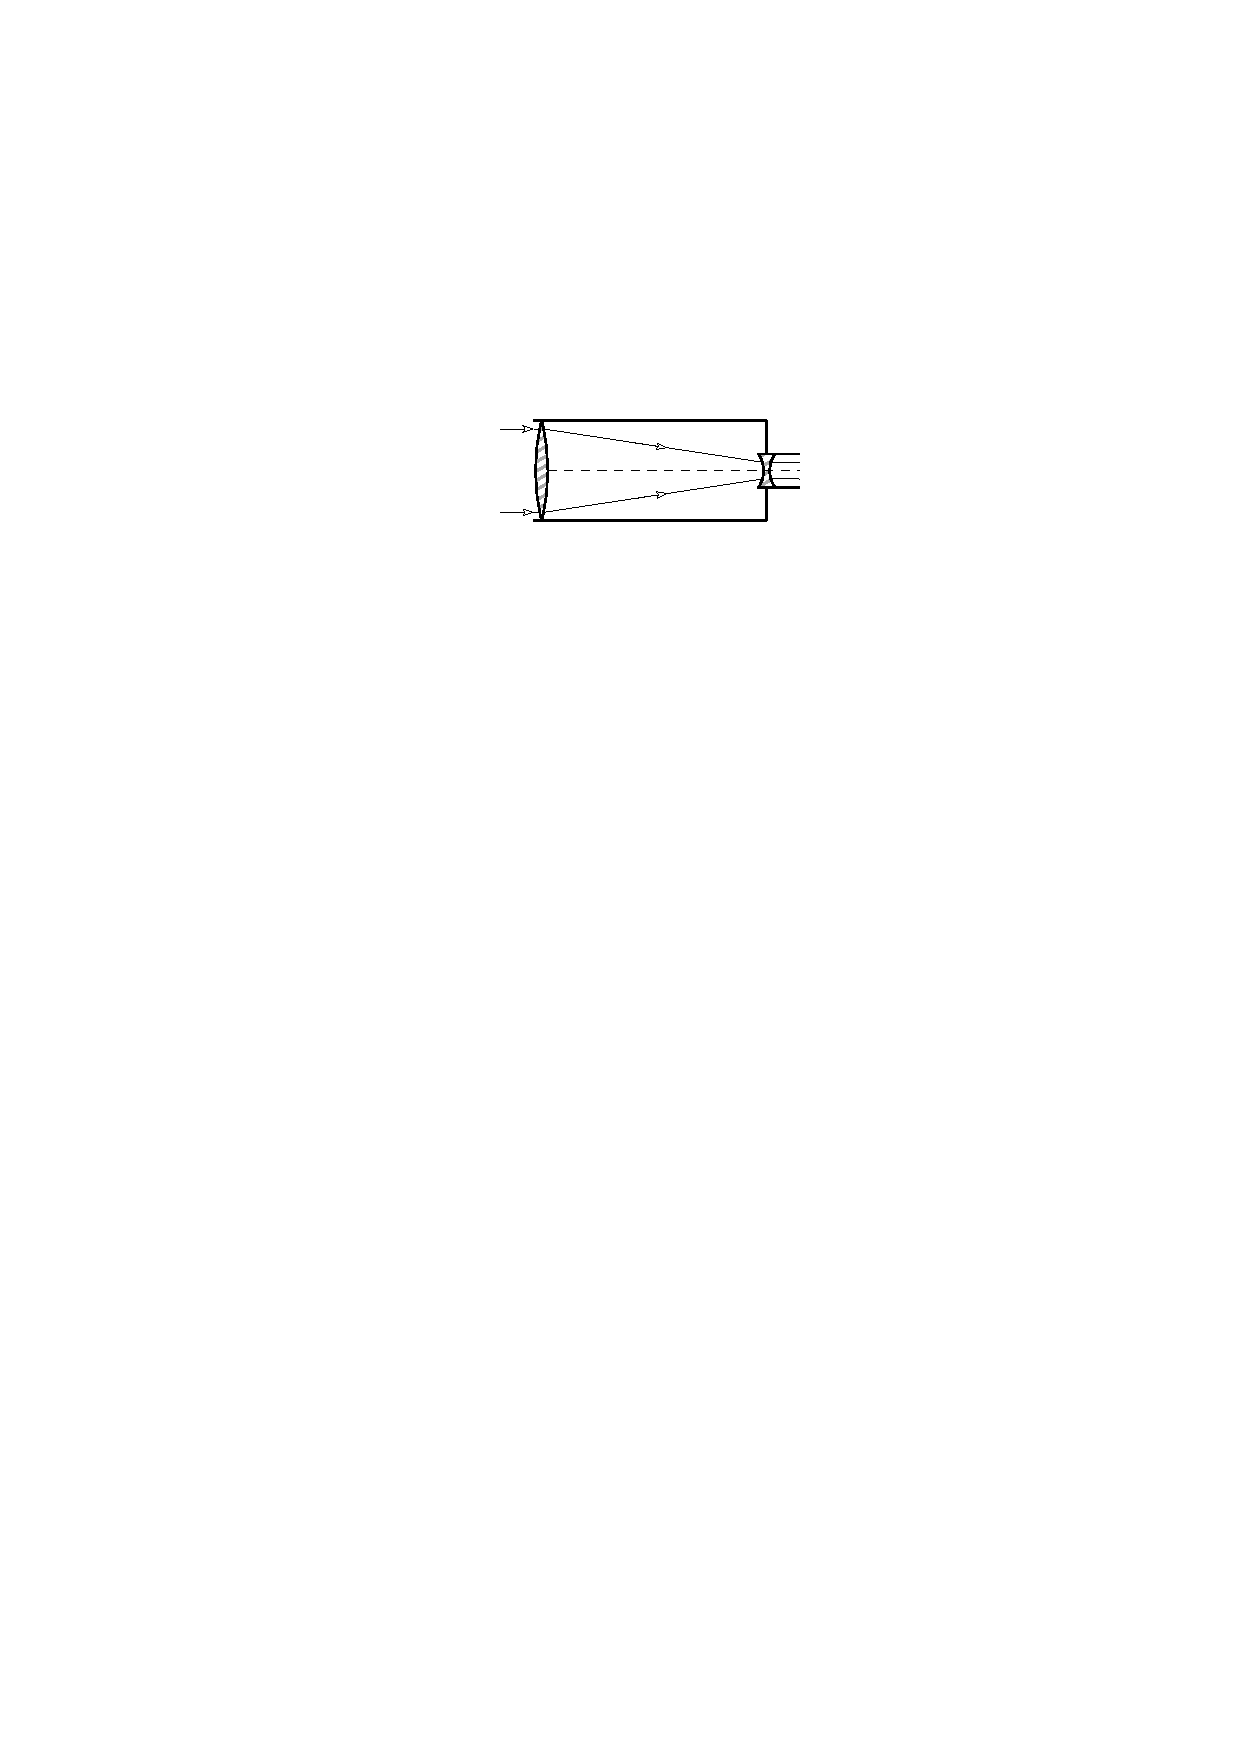
\includegraphics[width = \tw]{Galiley}
		\caption{Рефрактор системы Галилея}
	 \end{subfigure}
	 \hfill
	\begin{subfigure}{0.49\tw}
		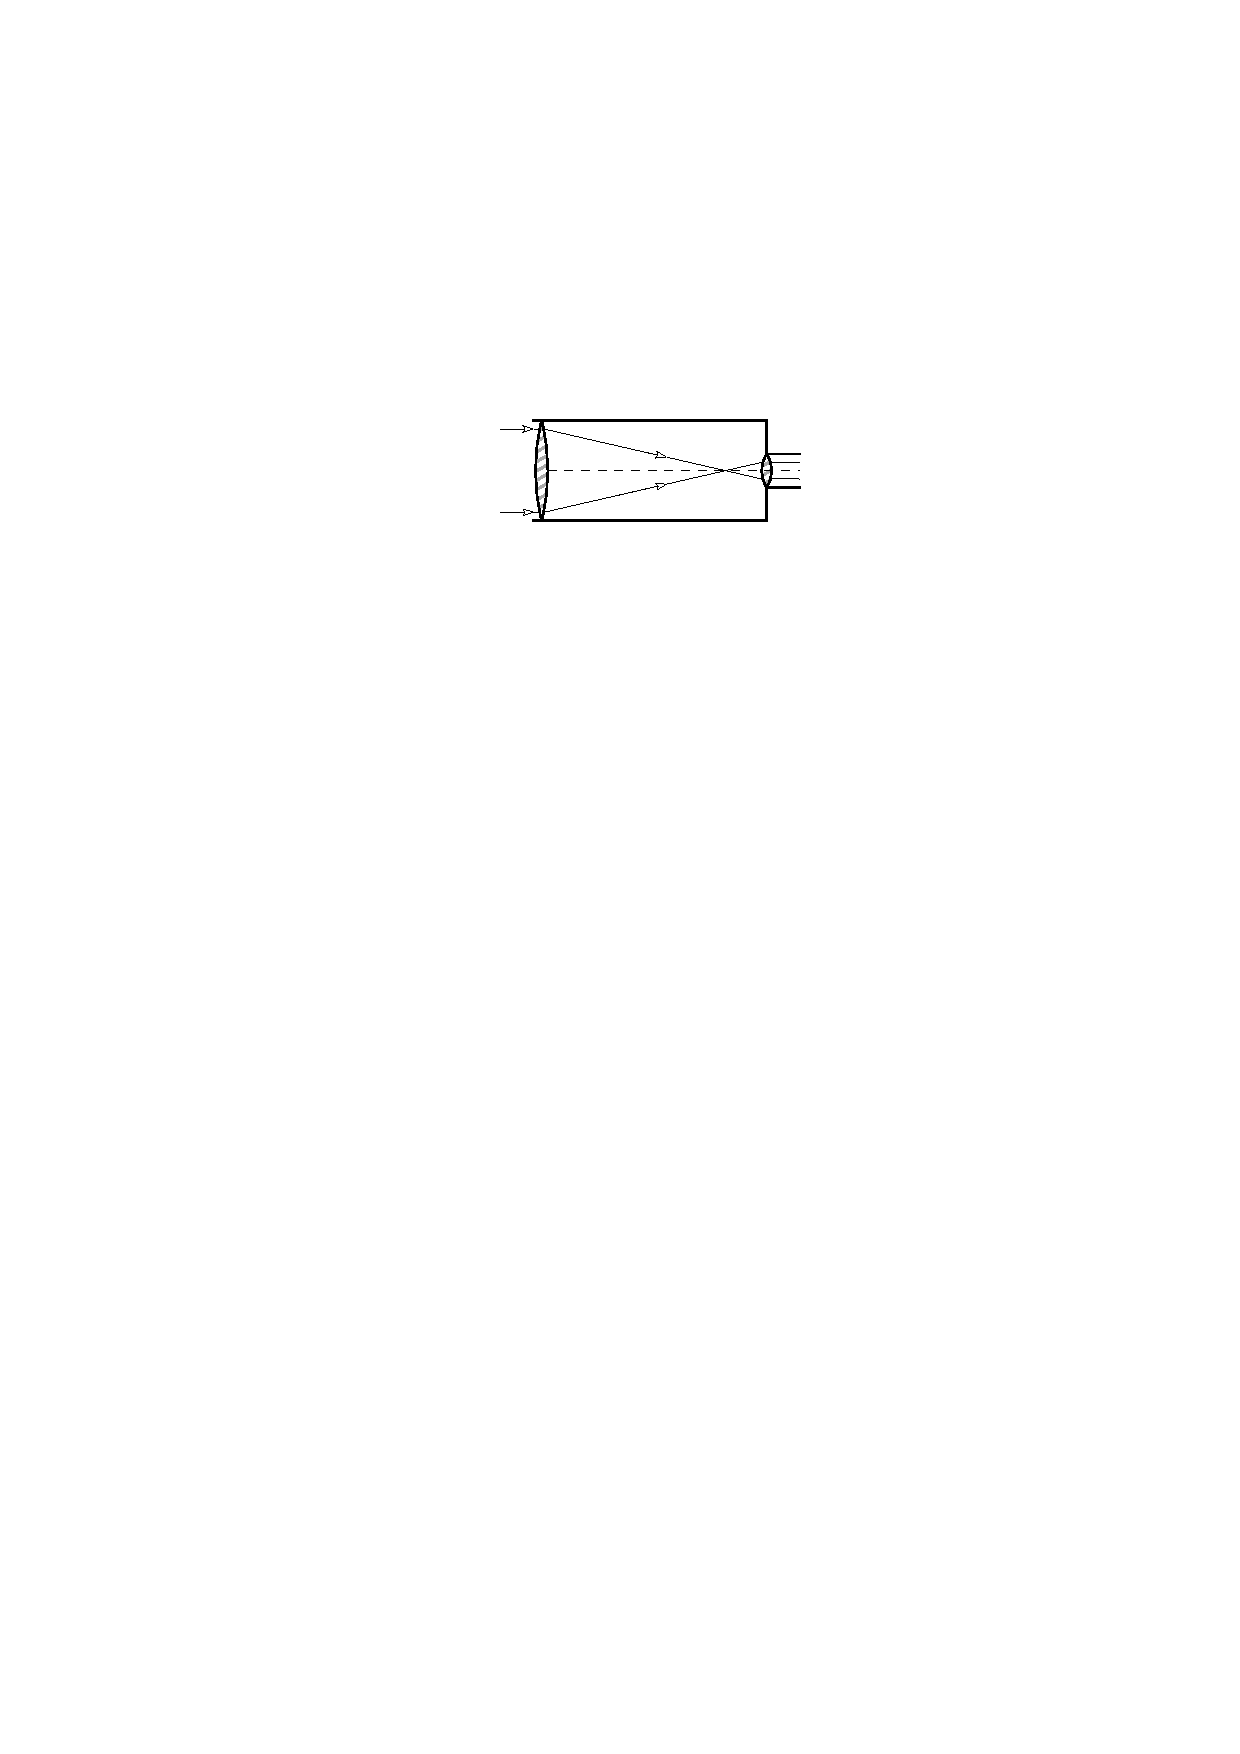
\includegraphics[width = \tw]{Kepler}
		\caption{Рефрактор системы Кеплера}
		 \label{Kepler}
	 \end{subfigure}
	 \caption{Оптические схемы телескопов рефракторов}
\end{figure}
\term{Рефрактор} (линзовый телескоп)~---  оптический телескоп, в котором для собирания света используется система линз.

\vspace{-.3pc}
\begin{figure}[h!]
	 \begin{subfigure}{0.49\tw}
		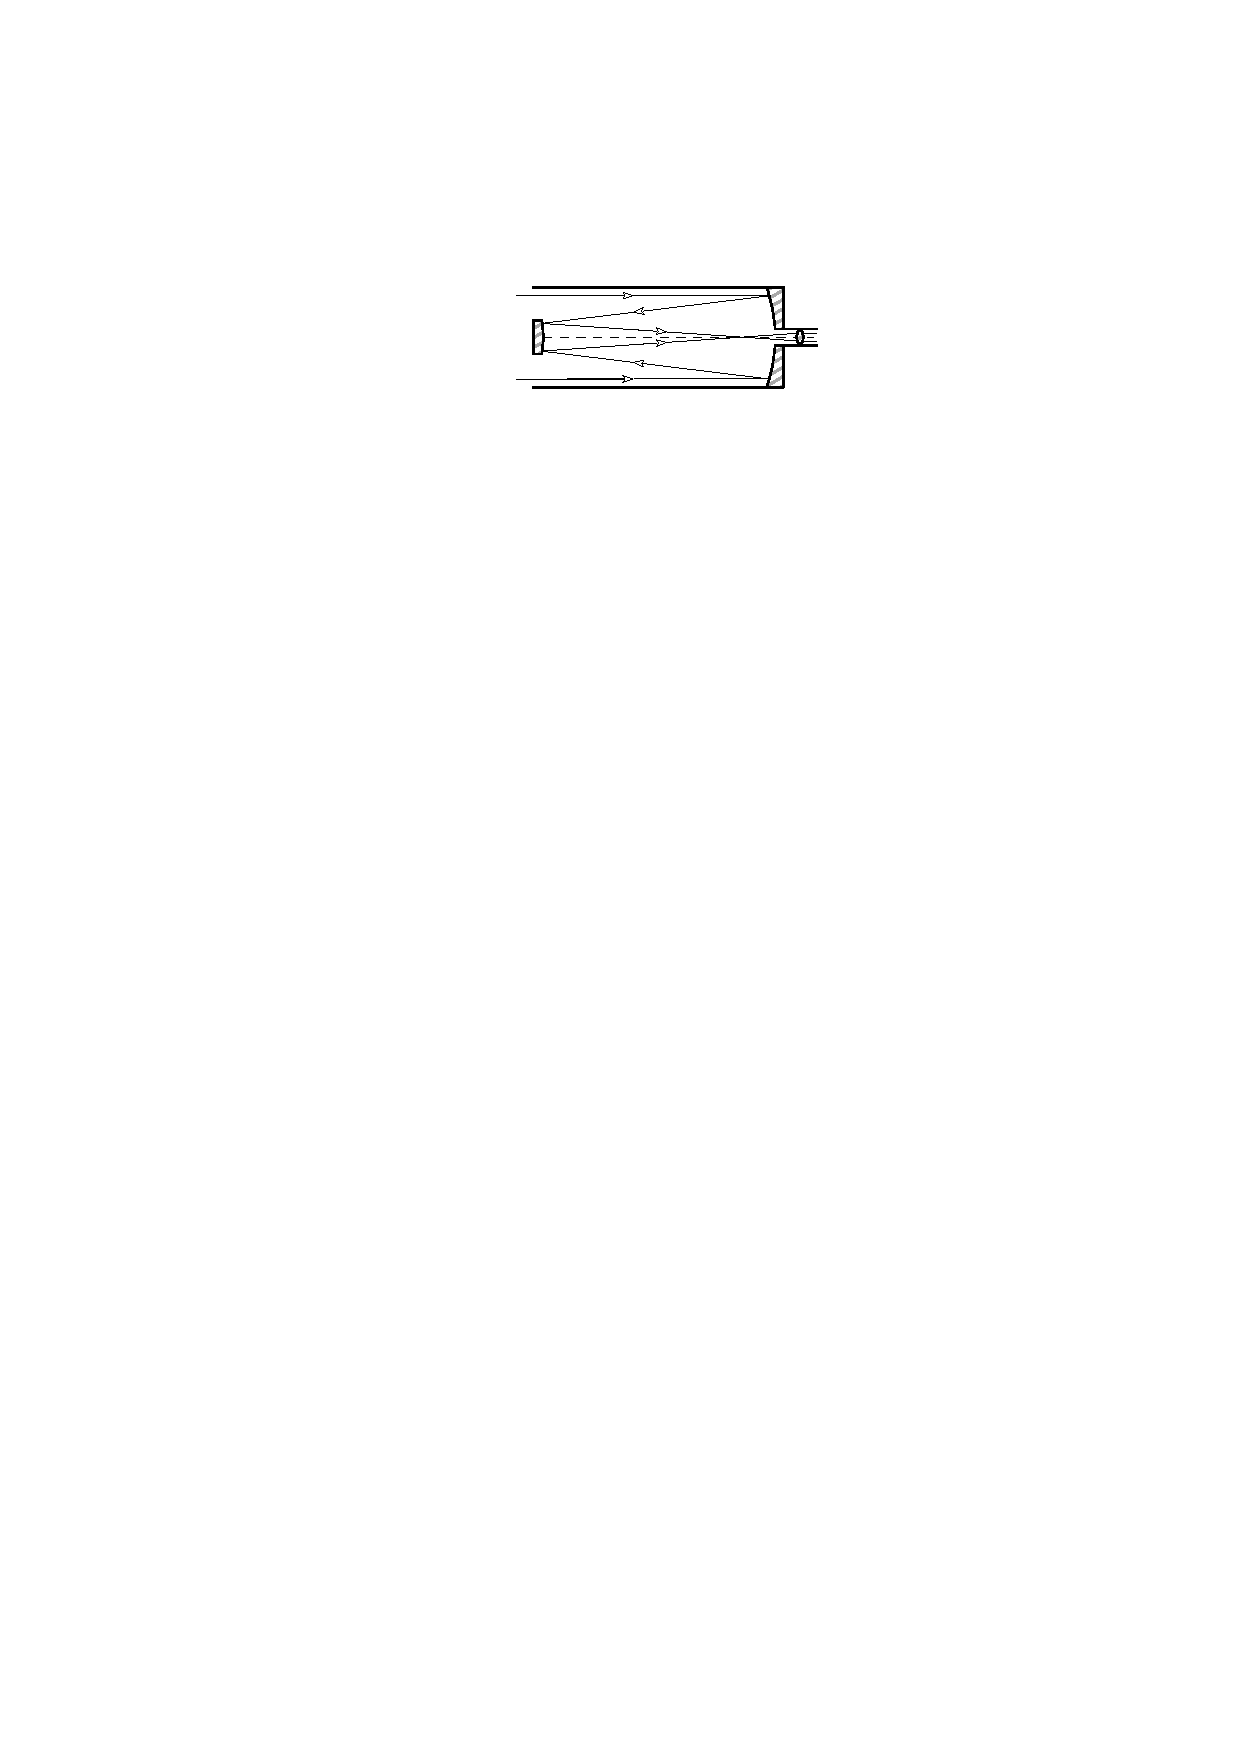
\includegraphics[width = \tw]{Cassigren.pdf}
		\caption{Рефлектор системы Кассегрена}
	 \end{subfigure}
	 \hfill
	 \begin{subfigure}{0.49\tw}
		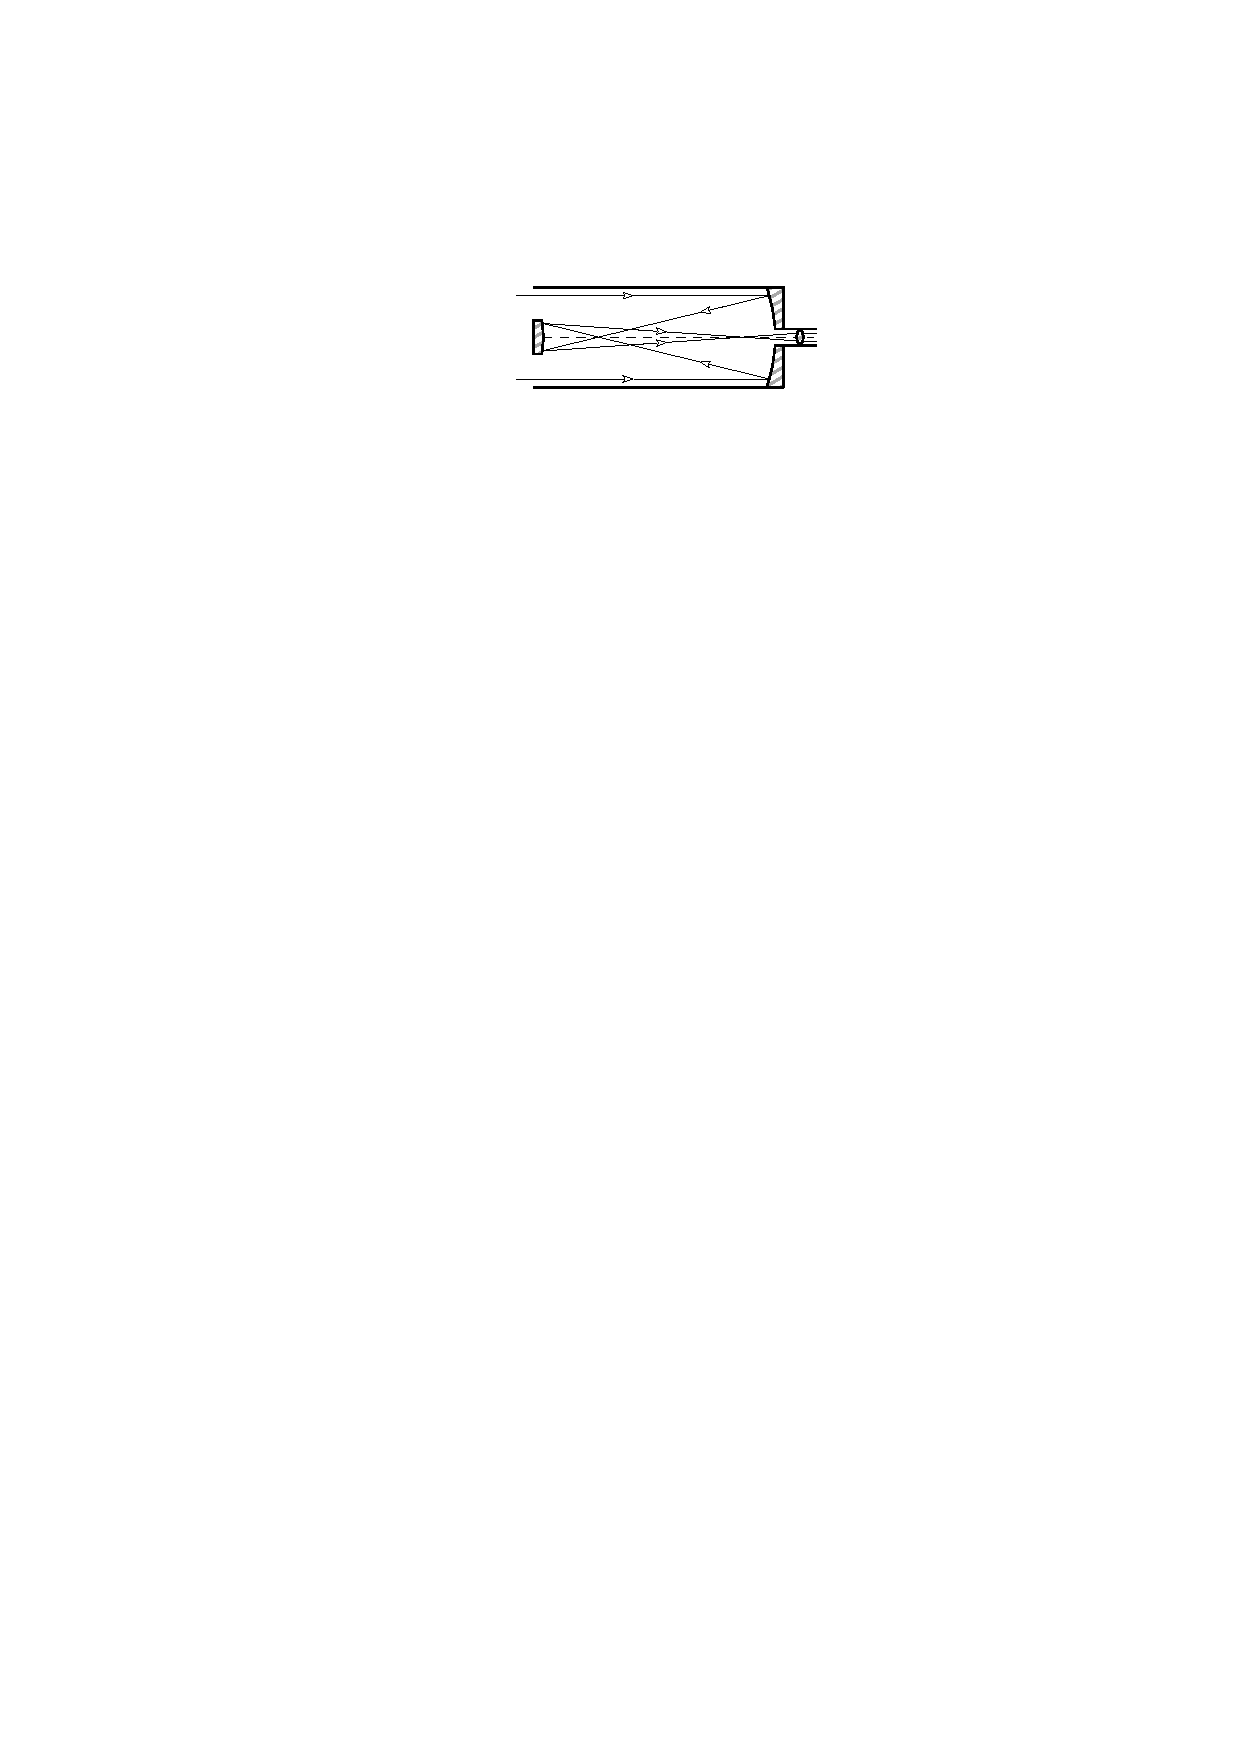
\includegraphics[width = \tw]{Gregory.pdf}
		\caption{Рефлектор системы Грегори}
		\label{Gregory}
	 \end{subfigure}
	 \vskip4pt
	\begin{subfigure}{0.49\tw}
		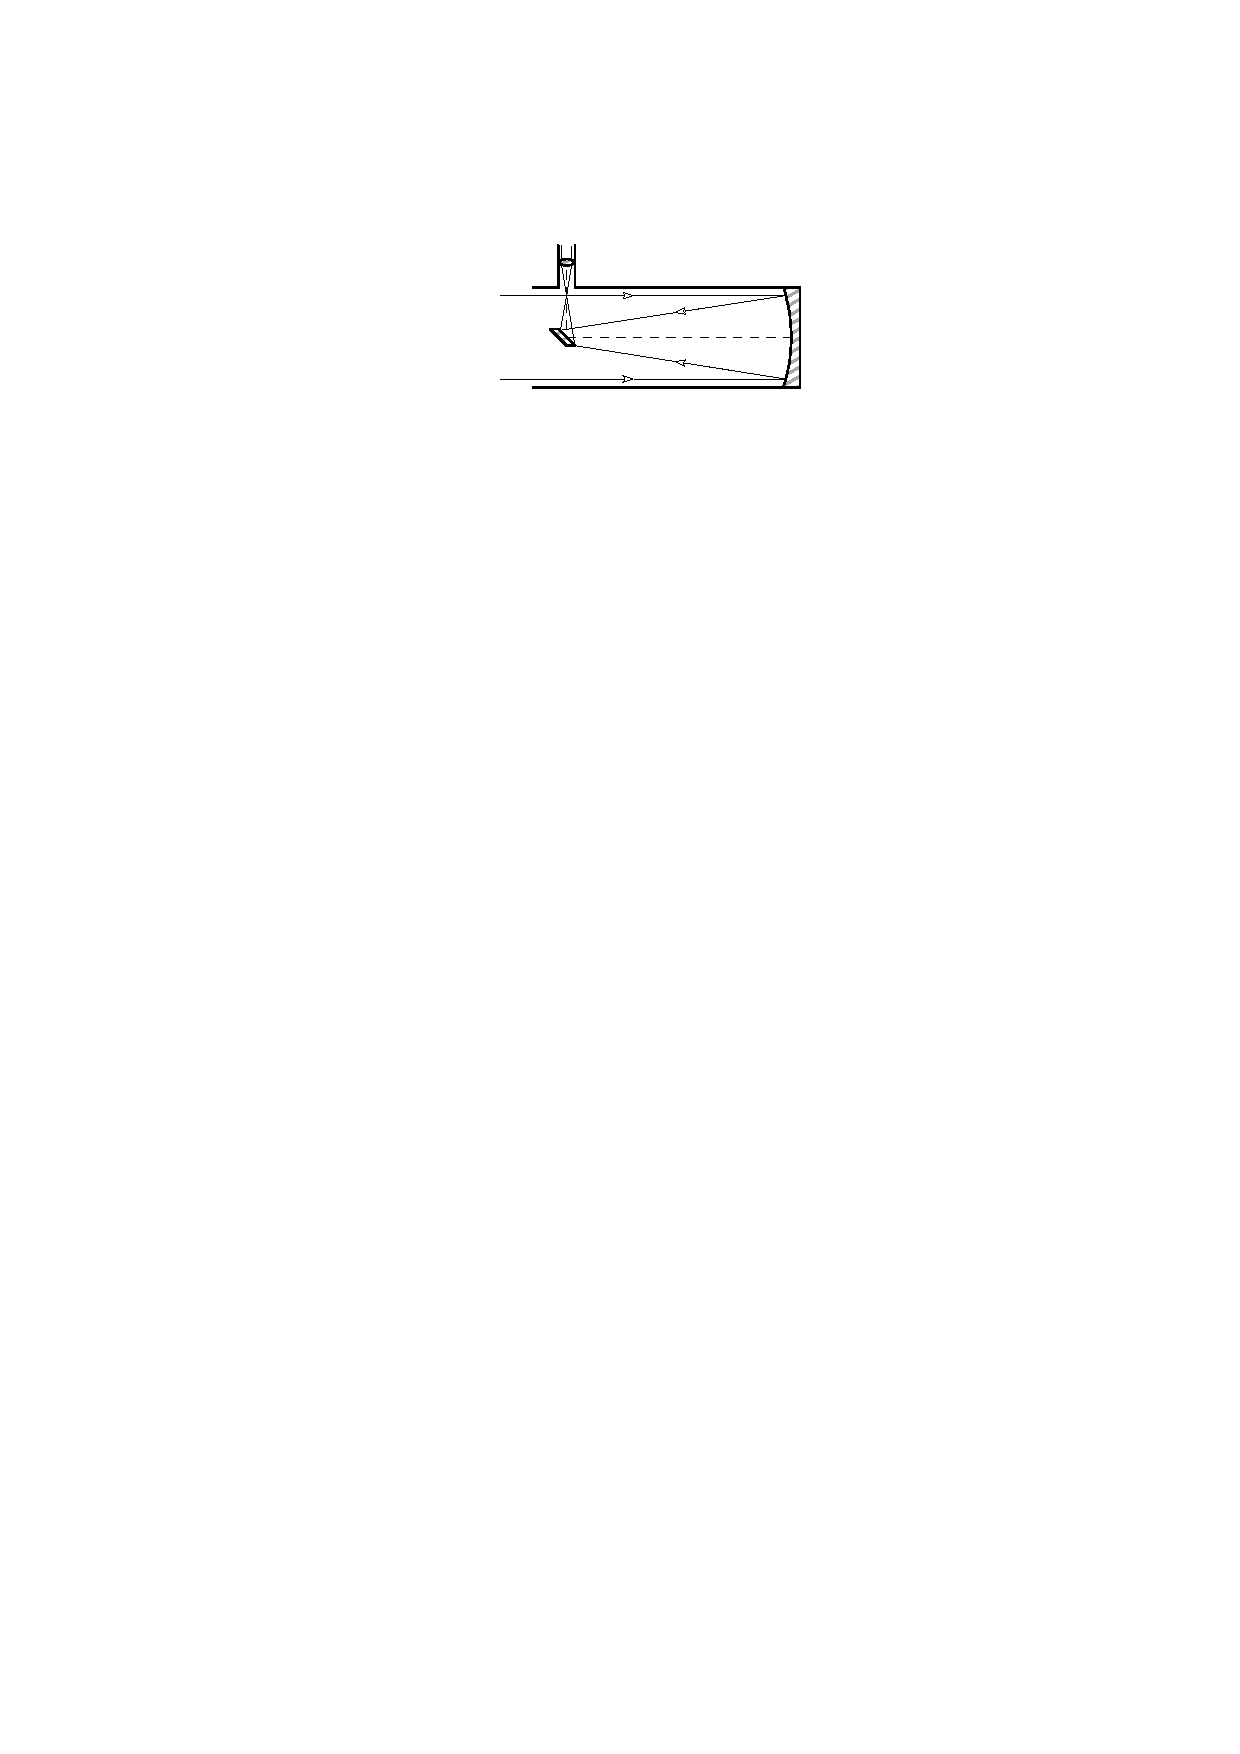
\includegraphics[width = \tw]{Newton}
 		\caption{Рефлектор системы Ньютона}
	\end{subfigure}
	\hfill
	\begin{subfigure}{0.49\tw}
		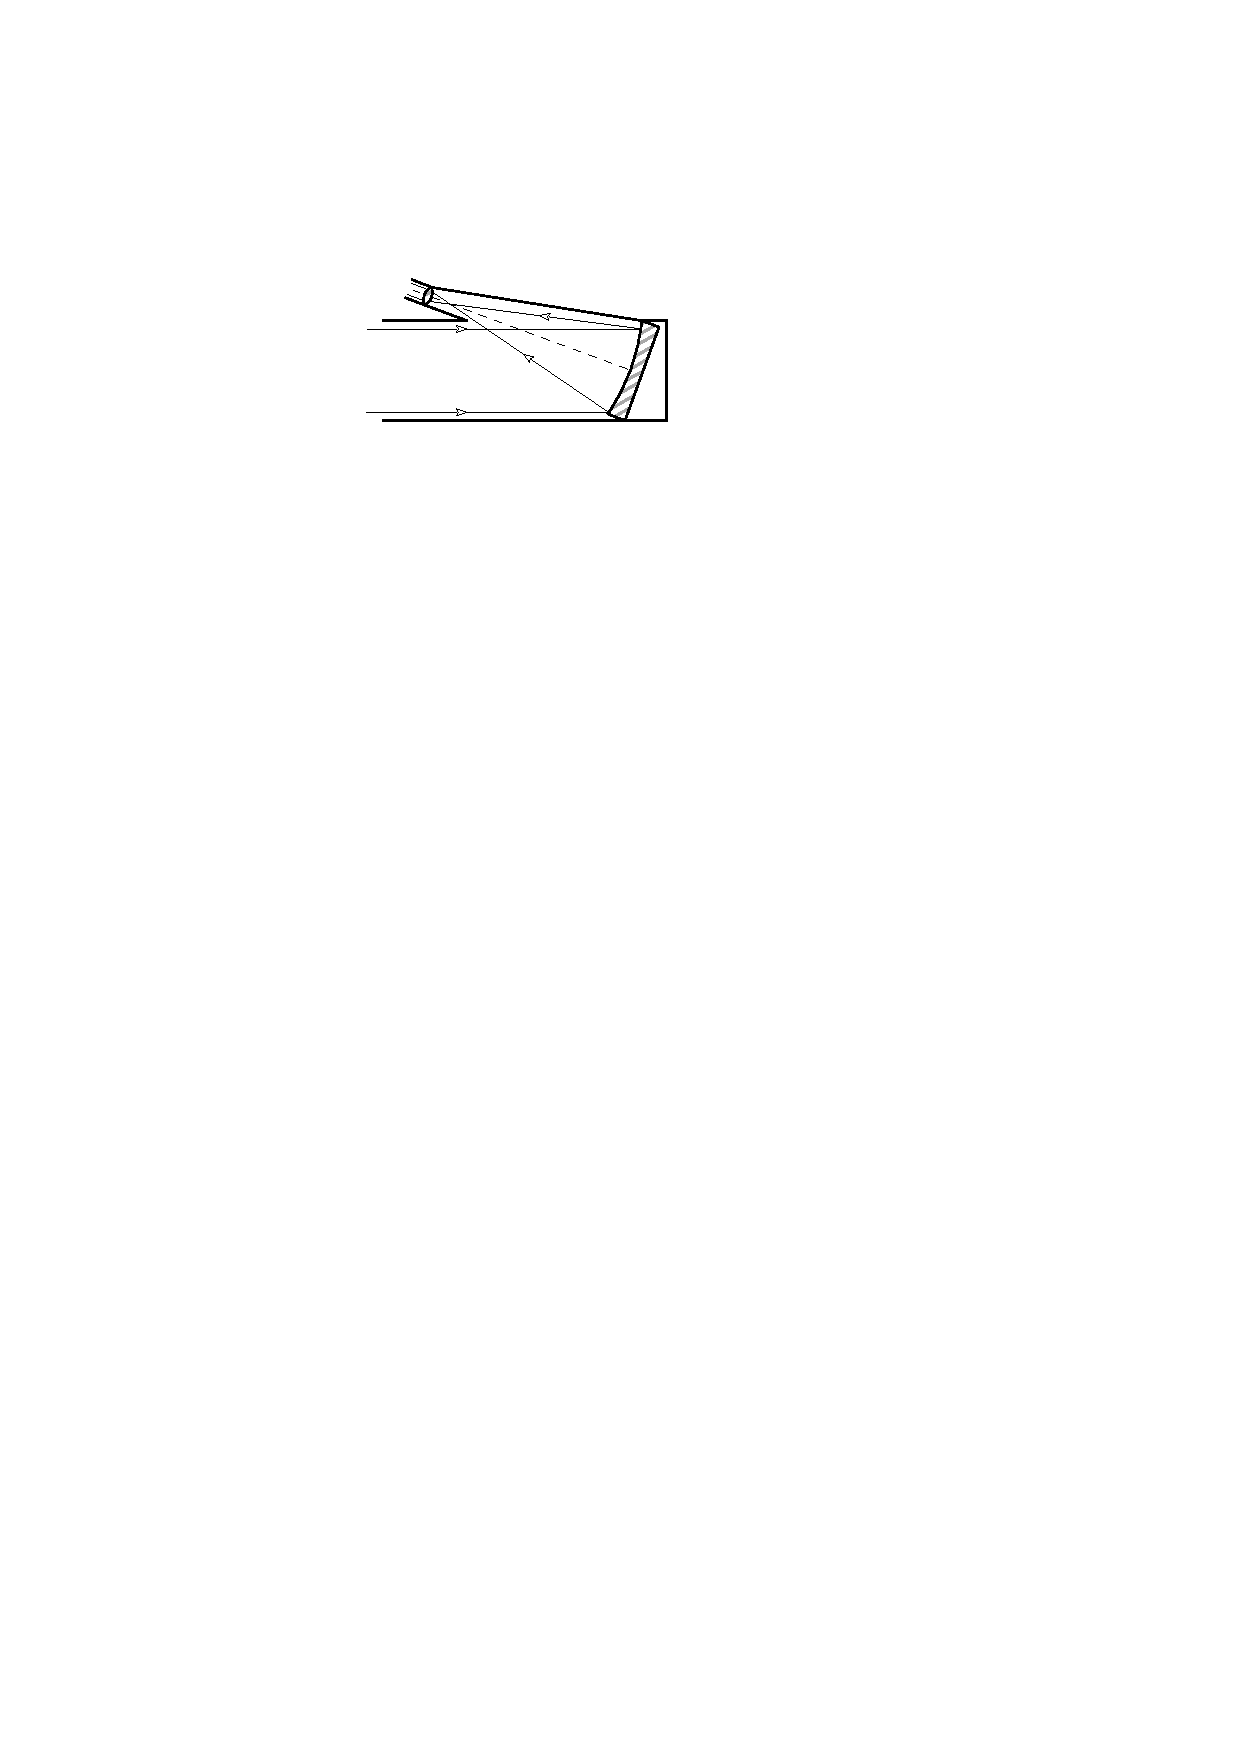
\includegraphics[width = \tw]{Lomonosov.pdf}
		\caption{Рефлектор системы Ломоносова}
	\end{subfigure}
	\caption{Оптические схемы телескопов рефлекторов}
\end{figure}
\term{Рефлектор} (зеркальный телескоп)~---  оптический телескоп,  в котором светособирающими элементами являются зеркала.

\term{Катадиоптрический} (зеркально-линзовый) \term{телескоп}~--- оптический телескоп, в котором используется как система линз, так и зеркал.
\subsection{Монтировки телескопов}
Монтировки телескопов разделяют на два основных вида: \imp{экваториальная} и \imp{альтзимутальная} монтировка (см.~Рис.\,\ref{mounts}).
\begin{figure}[h]
	\centering
	\hspace*{.4cm}
	\begin{subfigure}{0.48\textwidth}
		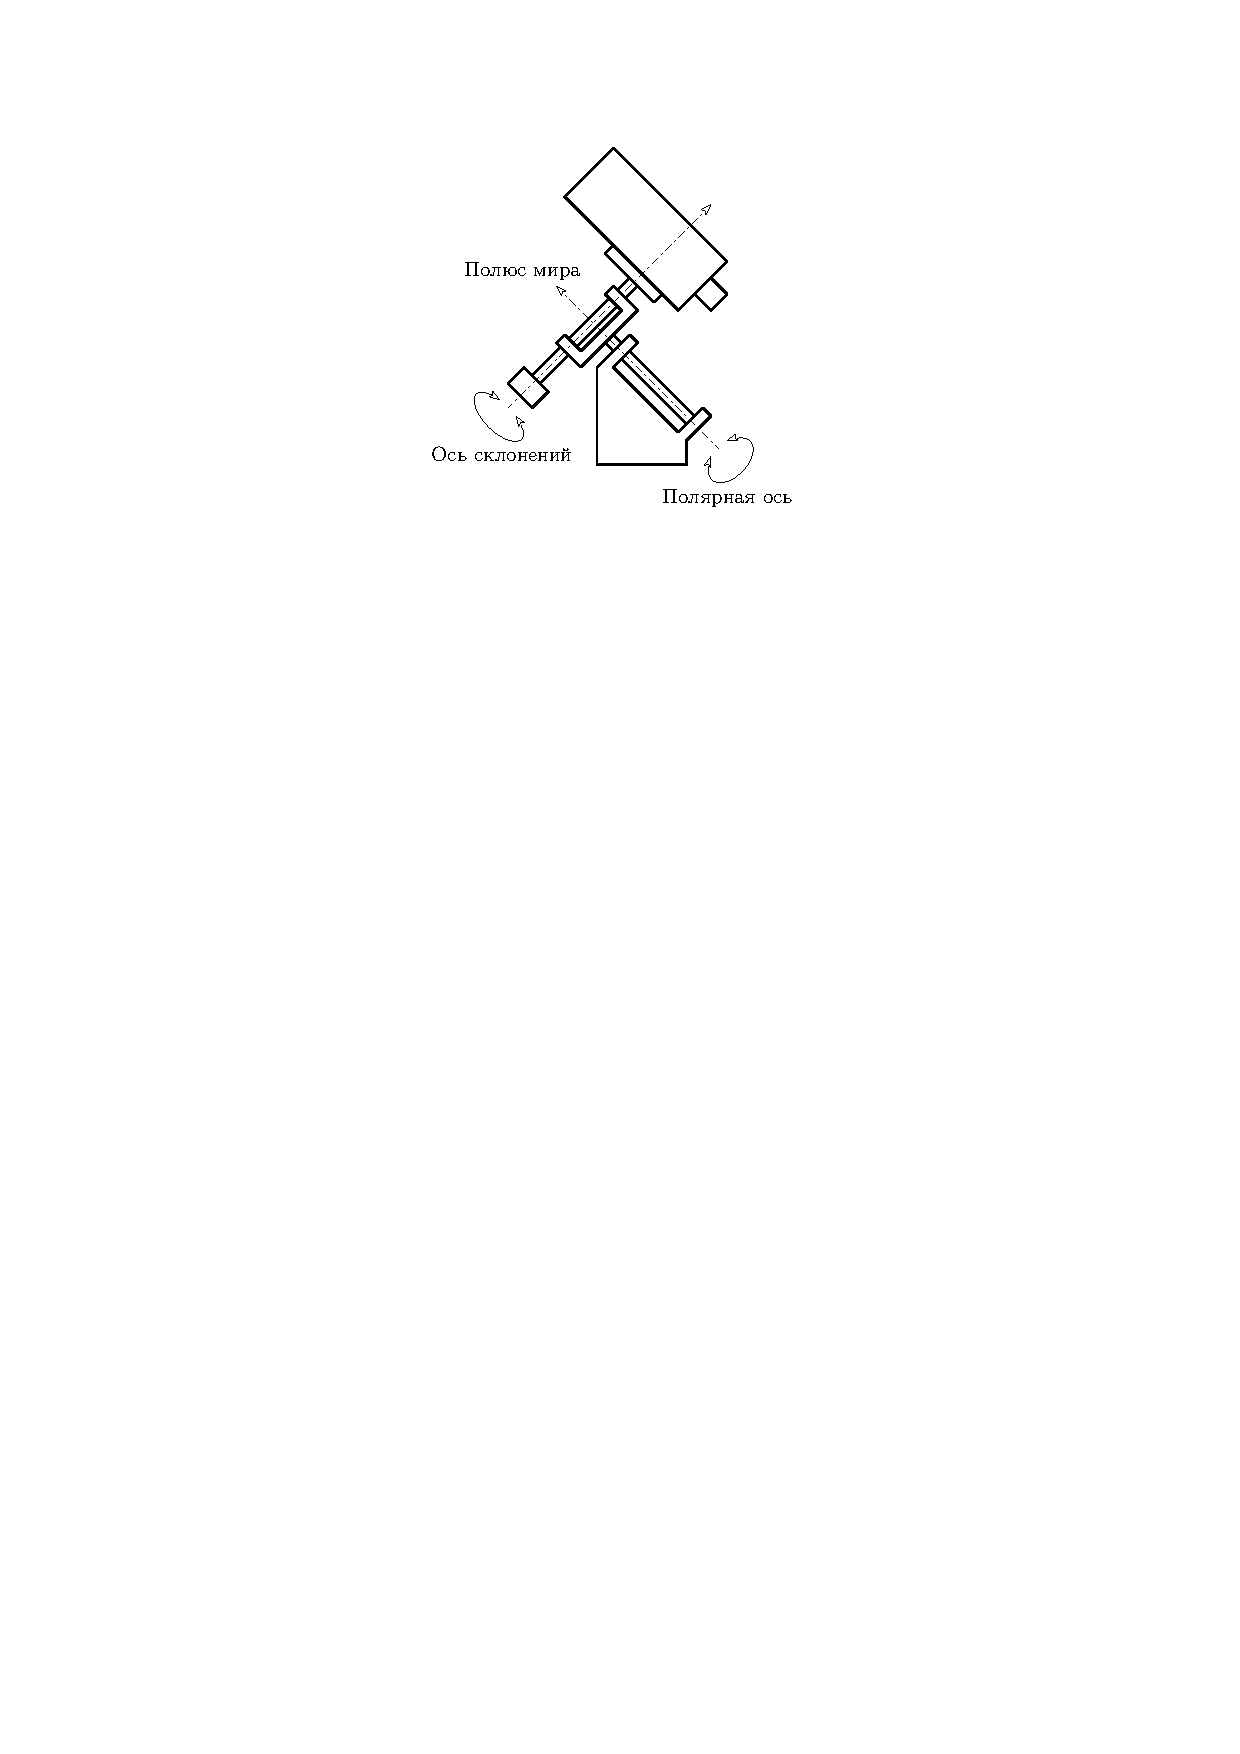
\includegraphics[height = 5cm]{mount-eq}
		\caption{Экваториальная мортировка}
	 \end{subfigure}
	\hspace*{.4cm}
	\begin{subfigure}{0.41\textwidth}
		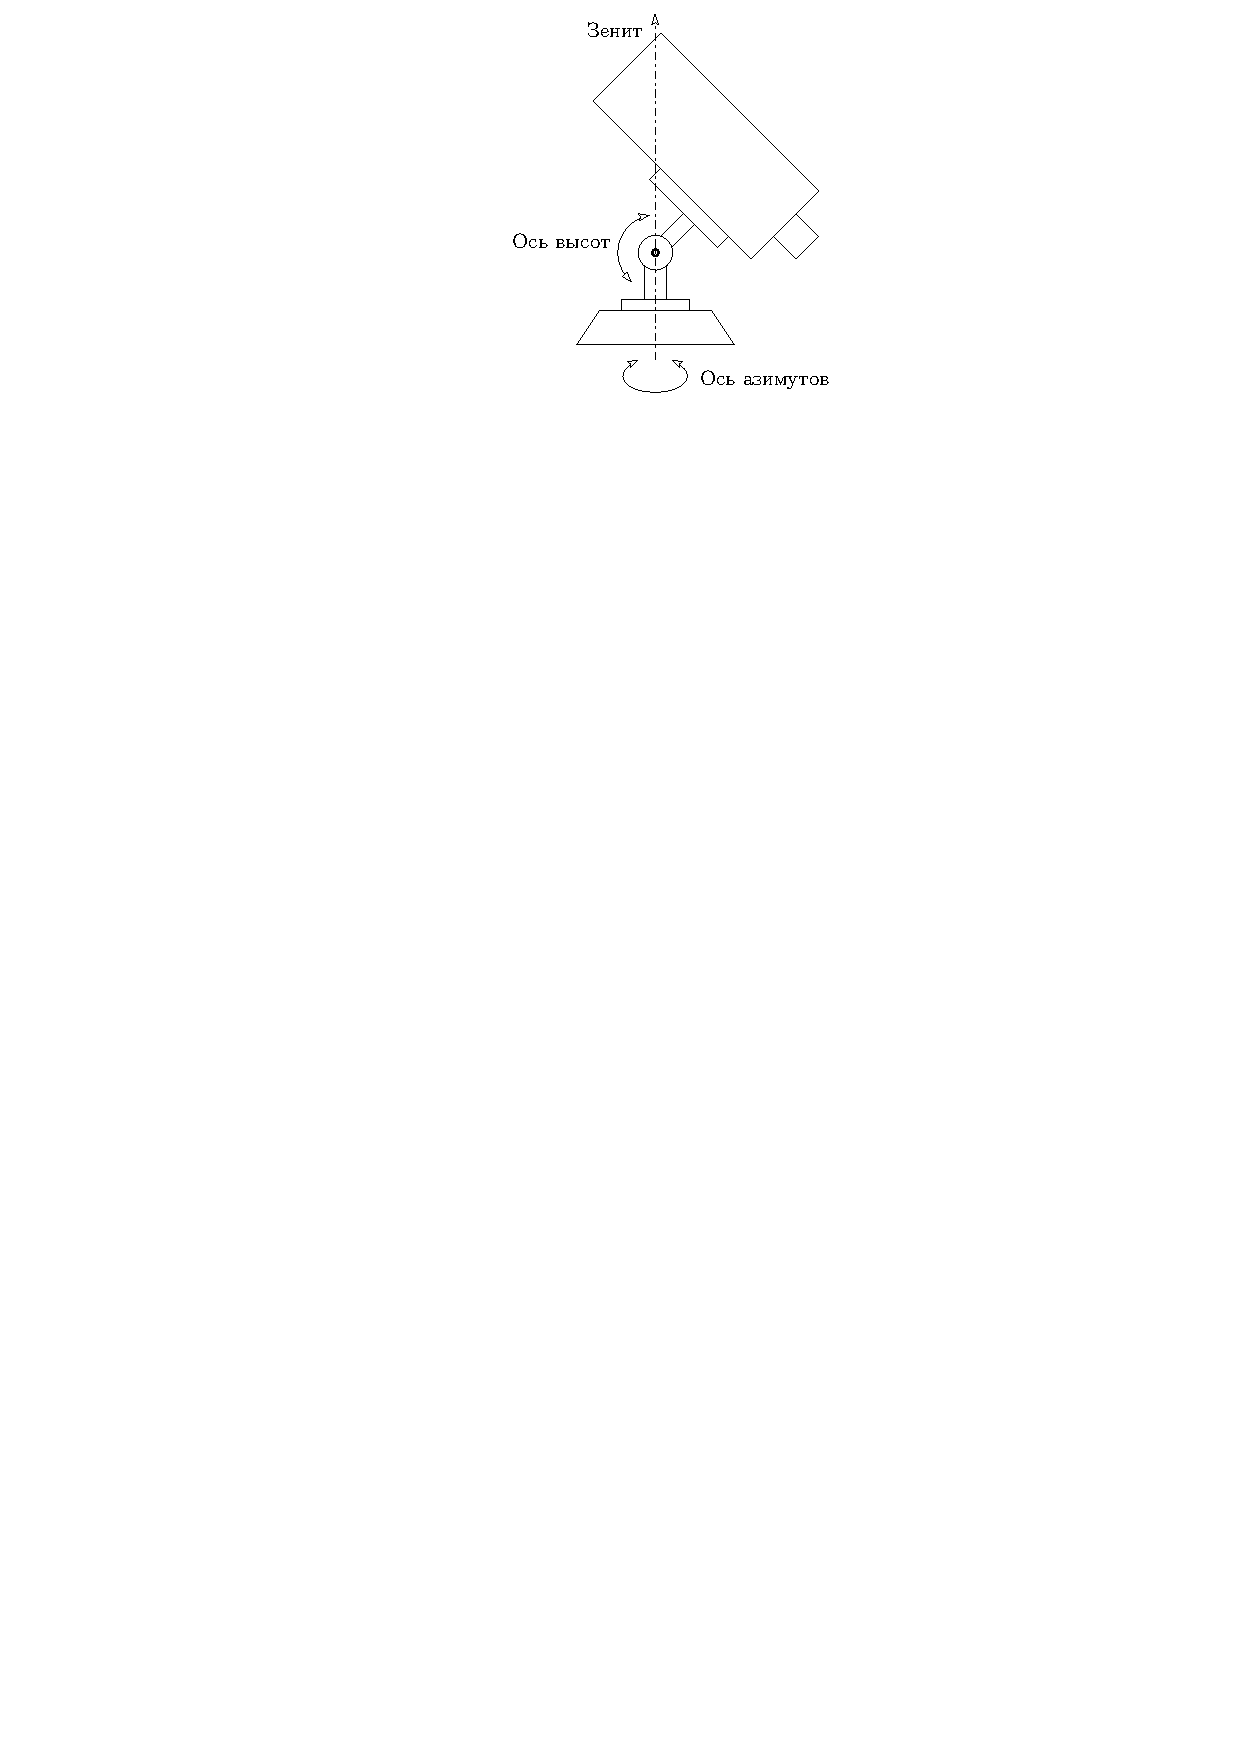
\includegraphics[height = 5cm]{mount-alt}
		\caption{Альтзимутальная монтировка}
	 \end{subfigure}
	 \hspace*{.4cm}
	 \caption{Виды монтировок}
	 \label{mounts}
\end{figure}

\term{Экваториальная монтировка}~--- монтировка, одна ось которой направлена на полюс мира (полярная ось), а другая параллельна небесному экватору (ось склонения). Для гидирования на такой монтировкой, нужно лишь поворачивать её с постоянной угловой скоростью вокруг полярной оси в направлении роста часового угла. Важно отметить, существует несколько разновидностей экваториальных монтировок: \imp{немецкая}, \imp{английская}, \imp{американская} монтировки и монтировка \imp{с рамой}.

\term{Альтзимутальная монтировка}~--- монтировка телескопа, имеющая вертикальную и горизонтальную оси вращения, позволяющие поворачивать телескоп по высоте и азимуту. Для слежения за космическими объектами, перемещающиеся по небесной сфере вследствие суточного вращения Земли, телескоп нужно поворачивать одновременно вокруг обеих осей с разными переменными скоростями.
\subsection{Параметры телескопа}
Из геометрической оптики известно, что лучи, проходящие через оптический центр линзы, не преломляются. Отсюда следует важное соотношение для линейного размера $l$ изображения объекта с угловым размером $\rho$ в фокальной плоскости:
\begin{equation}
	l = \rho F,
\end{equation}
здесь $F$~--- фокусное расстояние используемого телескопа.
Так как при помощи окуляра наблюдатель фактически смотрит на фокальную плоскость с расстояния $f$~--- фокусного расстояния окуляра, то угловой размер изображения, которое видит наблюдатель равно
\begin{equation}
	\alpha = \frac{l}{f}.
	\label{eq:zoom2}
\end{equation}
Следовательно, \term{увеличение телескопа}~$\Gamma$~--- отношение наблюдаемого и реального угловых размеров объекта равно отношению фокусных расстояний телескопа и окуляра. Из подобных треугольников также следует, что
\begin{equation}
	\Gamma =\frac{F}{f} = \frac{D}{d},
	\label{eq:zoom1}
\end{equation}
где $D$~--- диаметр входного зрачка (телескопа), $d$~--- диаметр выходного зрачка (окуляра). Важно отметить, что диаметры выходного и входного зрачка~--- диаметры пучков света, а не самих линз.

Увеличение называется \imp{равнозрачковым}, если диаметр выходного зрачка равен диаметру глазного зрачка наблюдателя, то есть
\begin{equation}
	\Gamma_\text{р.з.} = \frac{D}{d_\text{г}},
\end{equation}
где $d_\text{г}$~--- диаметр человеческого зрачка, обычно в тёмное время суток принимается за~6~мм.

Однако при росте увеличения детальность наблюдаемого изображения не улучшается. Происходит это в силу волновой природы света и, как следствие, явления \imp{дифракции} на входном отверстии телескопа. Наименьший угловой размер ещё различимых деталей определяется \term{разрешающей способностью} телескопа~--- это наименьшее угловое расстояние между двумя точечными объектами, при котором в телескоп ещё можно различить их раздельно. Предельное разрешение телескопа определяется формулой
\begin{equation}
	\beta = \frac{1.22\lambda}{D},
\end{equation}
где $\lambda$ --- длина волны наблюдений, при визуальных наблюдениях $\lambda \approx 550$~нм.

Кроме того, чем больше увеличение, тем меньше \term{поля зрения}~--- множество направлений, доступных для наблюдения. Из соотношений \eqref{eq:zoom2} и \eqref{eq:zoom1} следует зависимость \imp{поле зрения телескопа} $\alpha_\text{т}$ от \imp{поля зрения окуляра} $\alpha_\text{ок}$:
\begin{equation}
	\alpha_\text{т} = \frac{\alpha_\text{ок}}{\text{Г}},
\end{equation}
поле зрения стандартного окуляра составляет $45^\circ$.

Также, поле зрения телескопа можно вычислить, зная время $\tau$, за которое звезда со склонением $\delta$ пересекает поле зрения через его центр:
\begin{equation}
	\alpha_\text{т} = \frac{\tau \cos\delta}{4}.
\end{equation}

\term{Масштаб}~--- отношение углового размера объекта к линейному размеру его изображения на фокальной плоскости, следовательно
\begin{equation}
	\mu = \frac{\rho}{l} = \frac{\rho}{\rho F} = \frac{1}{F}=\left[\frac{\text{рад}}{\text{м}}\right].
\end{equation}

\term{Относительное отверстие}~--- геометрический параметр телескопа, равный отношению диаметра телескопа к его фокусному расстоянию
\begin{equation}
	\forall=\frac{D}{F}.
\end{equation}

\term{Светосила}~--- отношение освещенностей входного отверстия и фокальной плоскости, равна квадрату относительного отверстия.
\begin{equation}
	A=\forall^2=\frac{D^2}{F^2}.
\end{equation}

Пожалуй, самой важной характеристикой телескопа является то, насколько слабые объекты можно зафиксировать с его помощью. Эта величина называется \term{проницающей способностью телескопа}~--- это предельная звёздная величина объектов, которые доступны для наблюдения в данный телескоп. Чаще всего проницающая способность определяется из формулы Погсона \eqref{eq:Pogson-law} в ходе сравнения телескопа с глазом ($m_\text{г} \simeq 6^m$), однако здесь нужно учесть:
\begin{enumerate}
	\item Отношение площадей собирающих поверхностей.
	\item Диаметр выходного пучка может быть больше размера приёмника, тогда часть света теряется.
	\item Отношение времён экспозиций (выдержка глаза составляет около 0.3~сек).
	\item Отношение квантовых эффективностей\footnote{\term{Квантовая эффективность}~--- отношение мощности регистрируемого излучения к мощности подающего для единицы площади приемника.}.
	\item Прочие эффекты, возникающие в ходе фотографических наблюдений.
\end{enumerate}
При учёте только первых двух пунктов проницающая способность равна
\begin{equation}
	m_\text{т} = m_\text{г} + 5\lg\frac{D}{d_\text{г}} - 5\lg\max \left\{ \frac{d}{d_\text{г}}, 1\right\}.
\end{equation}

\subsection{Формула тонкой линзы}

\begin{wrapfigure}[9]{c}{0.6\tw}
	\centering
	\vspace{-1pc}
	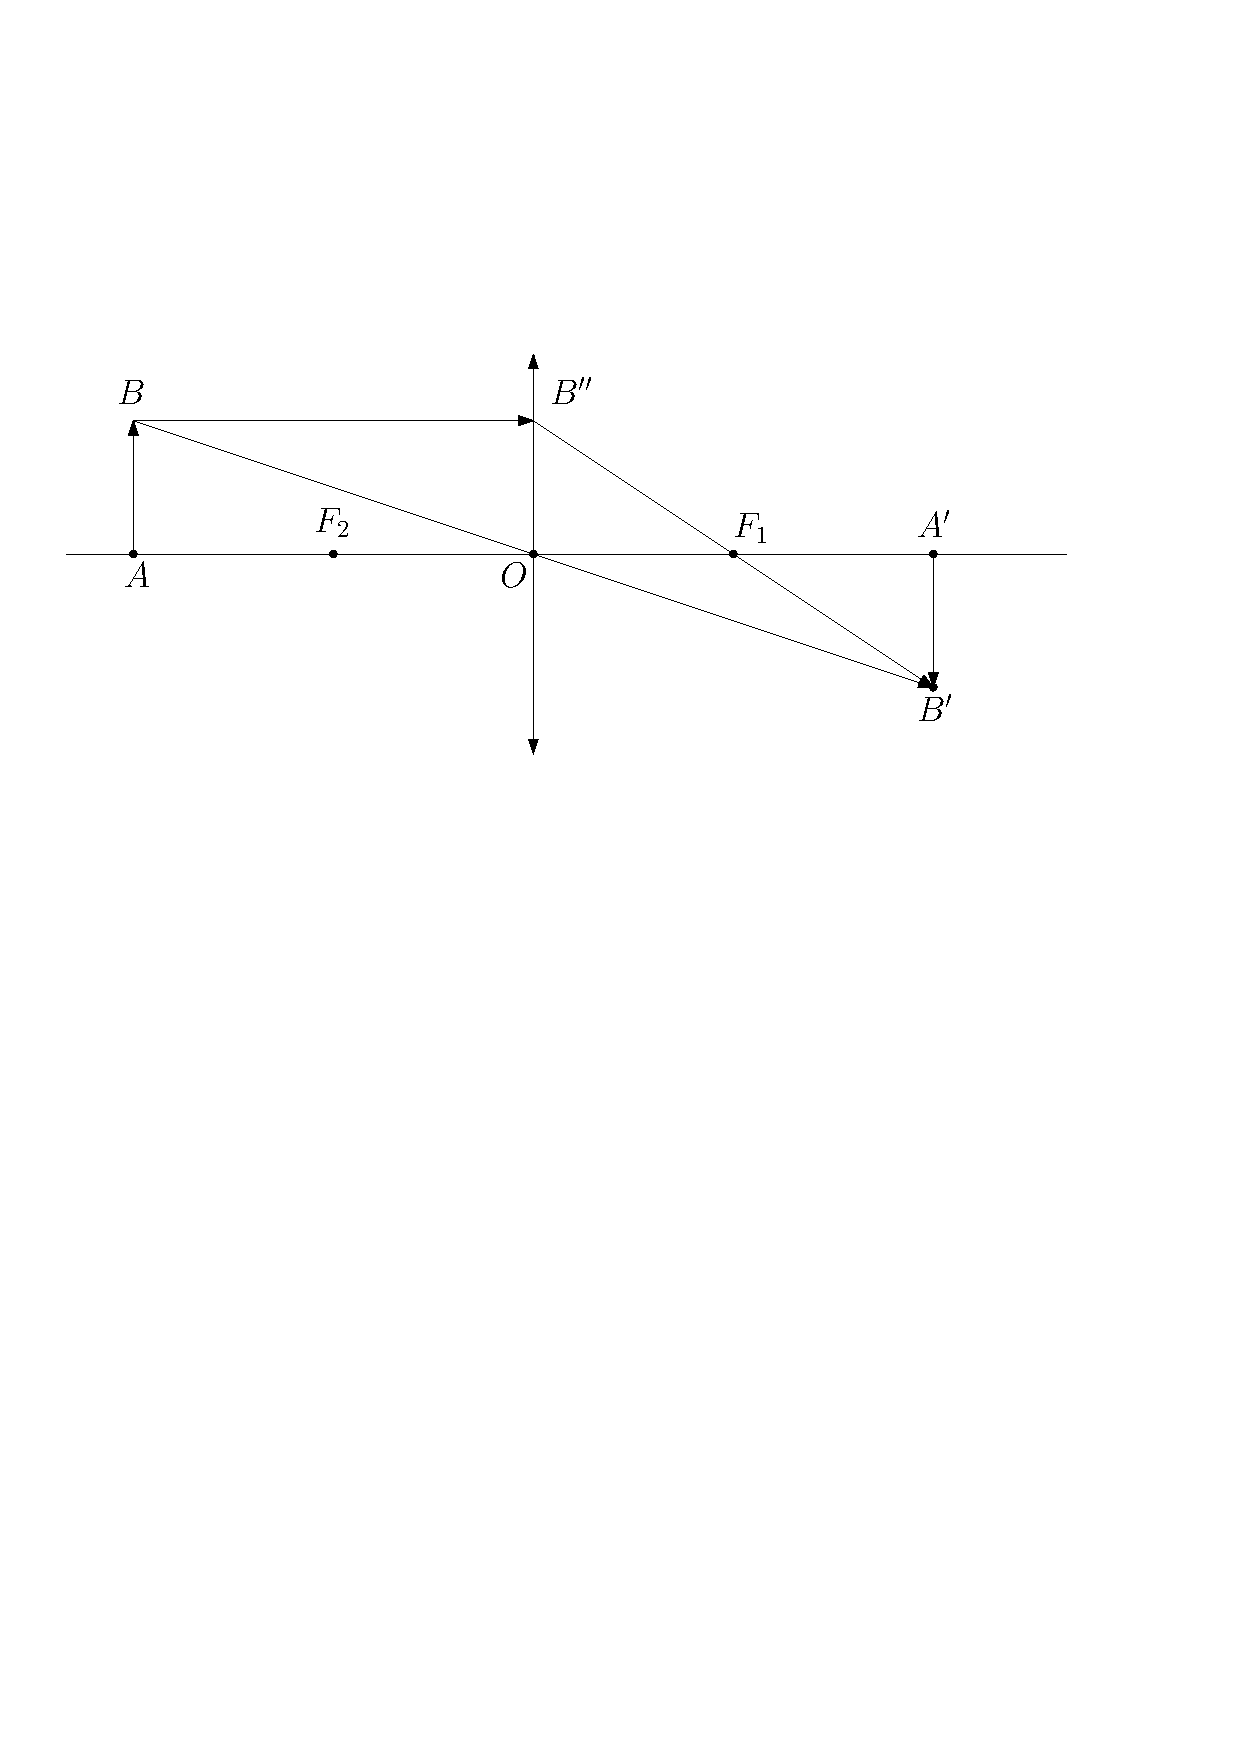
\includegraphics[width=.6\tw]{thin-lense}
	\captionof{figure}{Схема лучей в тонкой линзе}
	\label{fig:thin-lens}
\end{wrapfigure}

\change{
	Выведем формулу для связи расстояния от объекта до линзы, расстояния до изображения и фокусным расстоянием линзы.
	Введем обозначения: $F = OF_1 = OF_2$~--- фокусное расстояние линзы, $d = OA = BB^{\prime \prime}$~--- расстояние до объекта, $f = OA^\prime$~--- расстоние до изображения. 
	\begin{equation}
		\Delta ABO \sim \Delta A^\prime B^\prime O \Longrightarrow \frac{d}{f} = \frac{OB}{OB^\prime} = \frac{AB}{A^\prime B^\prime}
	\end{equation}
	\begin{equation}
		\Delta OB^{\prime \prime} F_1 \sim \Delta A^\prime B^\prime F_1 \Longrightarrow \frac{f - F}{F} = \frac{F_1 B^\prime}{OF_1} = \frac{A^\prime B^\prime}{OB^{\prime \prime}} = \frac{A^\prime B^\prime}{AB}
	\end{equation} 
	\begin{equation}
		\frac{f}{d} = \frac{f - F}{F} \Longrightarrow \frac{1}{d} = \frac{1}{F} - \frac{1}{f} \Longrightarrow \frac{1}{F} = \frac{1}{f} + \frac{1}{d}
	\end{equation}
	Полученная формула называется формулой тонкой линзой.
}
\subsection{Закон Снеллиуса}
Рассмотрим плоскую \imp{границу раздела} двух сред и луч, падающий на нее. Прямая, нормальная к плоскости раздела и проходящая через точку падения называется \imp{нормалью}. \term{Угол падение}~--- угол между нормалью и падающим лучем. В общем случае часть падающего излучения отражается от границы раздела, а часть проходит во вторую среду. \term{Углом отражения} называется угол между нормалью и отраженным лучем, а \term{углом преломления}~--- угол между нормалью и преломленным лучем.

Оптически прозрачная среда характеризуется скоростью распространения электромагнитного излучения (скоростью света) в ней. Скорость света в прозрачной среде определяется как
\begin{equation}
	c = \frac{c_0}{n},
\end{equation}
где $c_0$~--- скорость света в вакууме, а $n$~--- коэффициент преломления среды.

\term{Преломление}~--- изменение направления распространения волн (лучей) электромагнитного излучения, возникающее на границе раздела двух прозрачных для этих волн сред. Преломление света на границе двух сред даёт парадоксальный зрительный эффект: пересекающие границу раздела прямые предметы в более плотной среде ($n_1 >  n_2$) выглядят образующими больший угол с нормалью к границе раздела (то есть преломлёнными <<вверх»>>); в то время как луч, входящий в более плотную среду, распространяется в ней под меньшим углом к нормали (то есть преломляется <<вниз>>). Этот же оптический эффект приводит к ошибкам в визуальном определении глубины водоёма, которая всегда кажется меньше, чем есть на самом деле.

\begin{wrapfigure}[11]{r}{0.45\tw}
	\centering
	\vspace{-1pc}
	\begin{tikzpicture}
		\footnotesize
		
		\coordinate (0) at (0, 0) {};
		\coordinate (A) at (1.5, 0.87) {};
		\coordinate (2) at (2, 0) {};
		\coordinate (B) at (.13, -.5) {};
		
		%		\tkzMarkRightAngle[size=.4](0, A, 2);
		%		\tkzMarkRightAngle[size=.4](0, B, 2);
		
		\draw [double, line cap = butt] (0, -.7) arc(-90:-75:.7);
		\draw [double, line cap = butt] (1.3, 0) arc(180:195:.7);
		\draw [line cap = butt] (.5, 0) arc(0:30:.5);
		\draw [line cap = butt] (0, .5) arc(90:120:.5);
		
		\draw [line width = .5pt] (-1.5, 0) -- (3, 0);
		
		\draw [dashes] (0, -2) -- (0, 2);
		
		\draw [line width = 1pt] (-1.15, 2) -- (0, 0);
		\draw [line width = 1pt] (0.85, 2) -- (2, 0);
		\draw [line width = 1pt] (0.54, -2) -- (0, 0);
		\draw [line width = 1pt] (2.54, -2) -- (2, 0);
		\draw [line width = 1pt, -latex] (-1.15, 2) -- (-0.57, 1);
		\draw [line width = 1pt, -latex] (0.85, 2) -- (1.43, 1);
		\draw [line width = 1pt, -latex] (0, 0) -- (0.27, -1);
		\draw [line width = 1pt, -latex] (2, 0) -- (2.27, -1) ;
		
		\draw (0) -- (A);
		\draw (B) -- (2);
		
		\draw (3, 0) node [anchor=south east] {$n_1$};
		\draw (3, 0) node [anchor=north east] {$n_2$};
		\draw (0, .5) node [anchor=south east] {$\alpha$};
		\draw (.5, 0) node [anchor=south west] {$\alpha$};
		\draw (-.05, -.9) node [anchor=north west] {$\beta$};
		\draw (1, .06) node [anchor=north east] {$\beta$};
		
		вв	\end{tikzpicture}
		\caption{Ход лучей при прохождении границы раздела двух сред ввнаправлении из оптически менее плотной в оптически более плотную среду}
		\label{}
	\end{wrapfigure}
	Преломление света в атмосфере Земли приводит к тому, что мы наблюдаем восход Солнца несколько раньше, а закат несколько позже, чем это имело бы место при отсутствии атмосферы. По той же причине вблизи горизонта диск Солнца выглядит заметно сплющенным вдоль вертикали.
	
	Закон преломления называется \term{законом Снеллиуса}. Оставим его без доказательства в силу необходимой для этого теории, выходящей за рамки данного книги. Формулируется закон Снеллиуса так:
	\begin{equation}
		n_1 \sin \alpha = n_2 \sin \beta,
		\label{eq:snell-law}
	\end{equation}
	где $\alpha$~--- угол между лучем и нормалью в среде 1, $\beta$~--- в среде 2.
	
	Из \eqref{eq:snell-law} видно, что для некоторых $n_1$ и $n_2$ таких, что, например $n_2 > n_1$, и достаточно большом угле $\beta$ должно выполняться неравенство $\sin \alpha > 1$, что, очевидно, невозможно. Данная ситуация называется \imp{полным внутренним отражением}~--- всё излучение, падающее из более оптически более плотной среды, отразится от границы раздела. \term{Углом полного внутреннего отражения} называется такой минимальный угол $\beta$, при котором наблюдается полное внутреннее отражение. Положив $\sin \alpha = 1$, получаем, что
	\begin{equation}
		\sin \beta_\text{min} = \frac{n_1}{n_2}, \quad n_1 < n_2.
	\end{equation}

\subsection{Аберрации в оптике}
\paragraph{Сферическая аберрация}
В оптических системах, содержащих сферические поверхности (линзы, зеркала) может наблюдаться \imp{сферическая аберрация}. Суть такой аберрации в том, что лучи, параллельные оптической оси, идущие на разном расстоянии от нее собираются в разных её местах. Это приводит к тому, что на краях получаемого изображения, например, на ПЗС матрице, теряется резкость.

Покажем наличие сферической аберрации для плоско-выпуклой линзы. Важно отметить, здесь уже нельзя считать линзу тонкой, так как само по себе понятие тонкой линзы включает в себя условие фокусировки лучей в одной точке (фокусе), чего не происходит на практике. 

Итак, рассмотрим плоско-выпуклую линзу с радиусом выпуклой стороны $R$. Рассмотрим также луч, параллельный оптической оси этой линзы, на расстоянии $d$ от неё (см.~Рис.\,\ref{??}). Так как передняя поверхность линзы плоская, луч, попадая в линзу, не преломляется. Преломление происходит на выходе из линзы. Нетрудно показать, что для угла падения луча на заднюю поверхность линзы $\alpha$ справедливо, что $\sin \alpha = d/R$. По закону Снеллиуса угол преломления рассматримоего луча $\beta$ определяется соотношением $\sin \beta = n \sin \alpha$. Так как угол между нормалью к выпуклой поверхности линзы и ее оптической осью равен $\alpha$, то угол $\gamma$ между преломленным лучем и оптической осью линзы составляет $\beta - \alpha$.

Расстояние до точки пересечения преломленного луча с оптической осью линзы будем отсчитывать от вершины выпуклой поверхности. Расстояние $h(d)$ между проекцией точки преломления на оптическую ось и вершиной можно найти из теоремы Пифагора:
\begin{equation*}
	h(d) = R - \sqrt{R^2 - d^2}.
\end{equation*}
Тогда координата фокуса для лучей на расстоянии $d$ от оптической оси равно
\begin{equation*}
	x = \frac{d}{\tg \gamma} - h(d) = \frac{d}{\tg \left( \arcsin \dfrac{n d}{R} - \arcsin \dfrac{d}{R} \right)} - \left( R - \sqrt{R^2 - d^2} \right).
\end{equation*}
Введём обозначение $\delta \equiv d/R$ и разделим обе части полученного равенства на $R$, чтобы перейти к относительным единицам:
\begin{equation}
	\frac{x}{R} 
	= \frac{\delta}{\tg \left( \arcsin n\delta - \arcsin \delta \right)} -  1 + \sqrt{1 - \delta^2} 
	~\overset{\delta \ll 1}{\longrightarrow}~  \frac{1}{n - 1} - \frac{8\delta^2}{3}.\footnote{\scriptsize Вывод приближения:
\begin{multline*}
	\frac{\delta}{\tg \left( \arcsin n\delta - \arcsin \delta \right)} -  1 + \sqrt{1 - \delta^2} =\\
	= \frac{\delta}{\tg \left[ n \delta + \dfrac{n^3 \delta^3}{6} - \delta - \dfrac{ \delta^3}{6} + o(\delta^3) \right]} -  1 + \left(1 - \frac{\delta^2}{2} + o(\delta^2) \right) =\\
	= \frac{\delta}{\tg \left[ \delta(n-1) + \dfrac{(n^3-1) \delta^3}{6} + o(\delta^3) \right]} - \frac{\delta^2}{2} + o(\delta^2) =\\
	= \frac{\delta}{\delta(n-1) + \dfrac{(n^3-1) \delta^3}{6} + \dfrac{\delta^3}{3}(n-1)^3 + o(\delta^3)} - \frac{\delta^2}{2} + o(\delta^2) =\\
	= \frac{1/(n-1)}{1 + \dfrac{\delta^2}{6}(n^2 + n + 1) + \dfrac{\delta^2}{3}(n-1)^2 + o(\delta^2)} - \frac{\delta^2}{2} + o(\delta^2) =\\
	=\frac{1}{n-1} \left[1 - \frac{\delta^2}{6} (3n^2 -3n + 3) \right] - \frac{\delta^2}{2} + o(\delta^2) 
%	= \frac{1}{n-1} - \frac{\delta^2}{2(n-1)}(n^2 - n + 1 + n - 1) + o(\delta^2) 
	\simeq \frac{1}{n-1} - \frac{\delta^2 n^2}{2(n-1)}.
\end{multline*} 
}
\end{equation}
 

\begin{figure}[h!]
	\centering
	\begin{tikzpicture}
	\begin{axis}[
		height	=	6cm,
		width	=	8cm,
		xlabel	=	{$\delta$},
		ylabel	=	{$\dfrac{x(d)}{R}$},
		ylabel shift	= -1.1 cm,
		extra x ticks ={0.75},
    	extra x tick labels={$\frac{1}{n}$},
    	xmin=-.05,
    	xmax=0.8,
    	ymin=0,
    	ymax=3.5
		]
		\addplot[smooth] table[x=d, y=x] {data/shere-aberrations-lens.txt};
		\addplot[smooth] table[x=d, y=simple] {data/shere-aberrations-lens.txt};
		\addplot[dashes] coordinates { (0.75, -10) (0.75, 10)};
	\end{axis}
\end{tikzpicture}
\caption{}
\end{figure}

Найдём область определения функции $x(\delta)$. Прежде всего $\delta \geqslant 0$, потому что $d$~--- это расстояние от оптической оси, которое не может быть отрицательным. С другой стороны радиус линзы не может быть больше радиуса кривизны ее поверхности, следовательно, $\delta < 1$. Однако есть ещё одно условие, которое ограничивает $\delta$ сверху. Это эффект полного внутреннего отражения. Действительно, $\sin \beta$ не может быть больше единицы, следовательно, $\sin \alpha < \sfrac{1}{n}$, а значит, $\delta < \sfrac{1}{n}$. Для стекла, коэффициент преломления которого $n = \sfrac{4}{3}$, получаем, что $\delta \in [0, \sfrac{3}{4})$.

Как видно из графиков, приближение работает
\subsection{Диффракция}

Электромагнитное излучение берет свое название из принципа переноса энергии, который происходит в следствие колебаний электрического и магнитного полей. В случае одномерных гармонических колебаний уравнения Максвелла имеют такое решение:
\begin{align*}
	\vec E(x, t) &= \vec E_0 \cos (k x - \omega t + \varphi_0),\\
	\vec H(x, t) &= \vec H_0 \cos (k x - \omega t + \varphi_0). 
\end{align*}
Здесь $\vec E(x, t)$ и $\vec H (x, t)$~---  векторы напряженности электрического и магнитного полей соответственно с точке пространства с координатой $x$ в момент времени $t$. $E_0$ и $H_0$~--- амплитуды волн, которые связывает соотношение $\sqrt{\varepsilon}E_0 = \sqrt{\mu} H_0$. Остановимся на рассмотрении случая распространения излучения только в вакууме, тогда в СГС $E_0 = H_0$, так как в отсутствие среды $\varepsilon = \mu = 1$. \imp{Круговая частота} колебаний $\omega$ связана с обычной частотой колебаний $\nu$ соотношением $2\pi \nu = \omega$. А коэффициент $k$~--- \imp{волновое число}, определяемое, как $k = 2 \pi / \lambda$.

Такие волны, когда фаза волны в фиксированный момент времени зависит лишь от одной координаты, называют \imp{плоскими}. Остановимся на рассмотрении только таких волн.

Плотность потока энергии в электромагнитной волне определяется \imp{вектором Пойнтинга}:
\begin{equation}
	\vec{S} = \frac{c}{4\pi} \cross{E}{H}.
\end{equation}

Среднее значение вектора Пойнтинга называется \imp{интенсивностью излучения}:
\begin{equation}
	\vec I = \langle \vec S\rangle = \frac{c}{4\pi} \langle \cross{E}{H} \rangle.
\end{equation}
Для плоской волны в вакууме интенсивность равна
\begin{equation}
	I = \frac{c}{8\pi} E_0^2.
\end{equation}

\paragraph{Принцип Гюйгенса-Френеля}
\imp{Каждый элемент волнового фронта является центром возмущения, порождающего вторичные сферические волны, результат интерференции которых есть итоговое поле в каждой точке пространства.}

Воспользуемся данным принципом, чтобы найти поле от плоской волны после прохождения тонкой щели, то есть такой, что её ширина много меньше её длины. Пусть ширина щели равна $b$. Согласно принципу Гюйгенса-Френеля поле зависит только от угла между рассматриваемым направлением распространения излучения и осью щели. Пусть амплитуда падающей волны равна $A_0$. Тогда амплитуда от элемента ширины $dx$ в направлении $\theta$ определяется, как
\begin{equation*}
	dA = A_0 \cos (k x \sin \theta) \frac{dx}{b}.
\end{equation*}

Пусть $U \equiv k \sin \theta$, тогда суммарная амплитуда в направлении $\theta$ равна
\begin{multline*}
	A(\theta) 
	= \int dA 
	= \frac{A_0}{b} \int\limits_{-b/2}^{b/2} \cos ux\,dx =\\
	= \frac{A_0}{b} \left. \frac{\sin ux}{u} \right|_{-b/2}^{b/2} 
%	= \frac{A_0}{bu} \left( \sin \frac{ub}{2} - \sin \le- \frac{ub}{2} \right) = \\
	= \frac{A_0}{bu} \cdot 2 \sin \frac{bu}{2} = A_0 \left[ \sin \left( \frac{bu}{2}\right) \middle/  \frac{bu}{2} \right] .
\end{multline*}

Следовательно интенсивность определяется выражением
\begin{equation}
	I(\theta) = A^2(\theta) = A_0^2 \left[ \sin \left( \frac{bu}{2}\right) \middle/  \frac{bu}{2} \right]^2.
\end{equation}

Минимум данной функции достигается в точках, где обнуляется синус, то есть
\begin{gather*}
	\frac{bu}{2} = \pi m, \quad n \in \mathfrak Z;\\
	k \sin \theta = u = \frac{2 \pi m}{b},\\
	\sin \theta = \frac{2 \pi m}{bk} = \frac{2 \pi m \lambda}{2 \pi b},\\
	\theta \simeq \sin \theta = \frac{m \lambda}{b}.
\end{gather*}
Значит первый минимум находится на $\theta = \lambda/b$.

\begin{tikzpicture}
			\begin{axis}[
				height	=	4.125cm,
				width	=	5.5cm,
				xlabel	=	{$bu$, $\text{м}^2$},
				ylabel	=	{$I/A_0^2$},
				ylabel shift	= -1 cm,
				]
				
				\addplot[smooth, domain=-10:10, samples=200] {(sin(deg(x))/x)^2};
			\end{axis}
		\end{tikzpicture}



\begin{figure}[p]
	\centering
	\begin{subfigure}{\tw}
		\begin{tikzpicture}
			\begin{axis} [
				width			=	10cm,
				colormap 		= 	{GS}{rgb(0cm)=(.1, .1, .1)  rgb(1cm)	=	(1, 1, 1)},
				xlabel 			=	{$x$, $\frac{\lambda}{D}$},
				ylabel 			=	{$y$, $\frac{\lambda}{D}$},
				zlabel 			=	{$I/I_0$},
				ylabel shift 	= -.4 cm,
				xlabel shift 	= -.3 cm,
				ytick			= {-2,0,2},
				colorbar,
				colorbar style 	= {
				ytick 	= 	{0, .2, .4, .6, .8, 1.},
				}
				]
				
				\addplot3[
				samples				=	100,
				samples y			=	100,
				mesh,
				patch type			=	line,
				x filter/.code		=	\def\pgfmathresult{-5},
				smooth
				]
				table[x=x, y=y, z=I] {data/eiry-disk-x.txt};
				%
				\addplot3[
				samples			=	100,
				samples y		=	100,
				mesh,
				patch type		=	line,
				y filter/.code	=	\def\pgfmathresult{4.5},
				smooth
				]
				table[x=x, y=y, z=I] {data/eiry-disk-y.txt};
				
				\addplot3[surf] table[x=x, y=y, z=I] {data/eiry-disk.txt};
			\end{axis}
		\end{tikzpicture}
		\caption{}
		\label{}
	\end{subfigure}\\[2pc]
	\begin{subfigure}{\tw}
		\begin{tikzpicture}
			\begin{axis} [
				width			=	10cm,
				height			=	7.5cm,
				colormap 		= 	{GS}{rgb(0cm)=(.1, .1, .1)  rgb(1cm)	=	(1, 1, 1)},
				view			=	{0}{90},
				ytick 	= 	{-3, -2, ..., 3},
				colorbar,
				colorbar style 	= 	{
				ytick 	= 	{0, .2, .4, .6, .8, 1.},
				},
				xlabel 			=	{$x$, $\frac{\lambda}{D}$},
				ylabel 			=	{$y$, $\frac{\lambda}{D}$},
				]
				
				\addplot3[surf, shader=interp] table[x=x, y=y, z=I] {data/eiry-disk.txt};
			\end{axis}
		\end{tikzpicture}
		\caption{}
		\label{}
	\end{subfigure}
	\caption{}
\end{figure}

\begin{figure}[p]
	\centering
	\begin{subfigure}{\tw}
		\begin{tikzpicture}
			\begin{axis} [
				width			=	10cm,
				colormap 		= 	{GSW}{rgb(0cm)=(.1, .1, .1) rgb(.05cm)=(.99, .99, .99) rgb(1cm)	=	(1, 1, 1)},
				xlabel 			=	{$x$, $\frac{\lambda}{D}$},
				ylabel 			=	{$y$, $\frac{\lambda}{D}$},
				zlabel 			=	{$I/I_0$},
				ylabel shift 	= -.4 cm,
				xlabel shift 	= -.3 cm,
				ytick			= {-2,0,2},
				colorbar,
				colorbar style 	= {
				ytick 	= 	{0, .2, .4, .6, .8, 1.},
				}
				]
				
				\addplot3[
				samples				=	100,
				samples y			=	100,
				mesh,
				patch type			=	line,
				x filter/.code		=	\def\pgfmathresult{-5},
				smooth
				]
				table[x=x, y=y, z=I] {data/eiry-disk-x.txt};
				%
				\addplot3[
				samples			=	100,
				samples y		=	100,
				mesh,
				patch type		=	line,
				y filter/.code	=	\def\pgfmathresult{4.5},
				smooth
				]
				table[x=x, y=y, z=I] {data/eiry-disk-y.txt};
				
				\addplot3[surf] table[x=x, y=y, z=I] {data/eiry-disk.txt};
			\end{axis}
		\end{tikzpicture}
		\caption{}
		\label{}
	\end{subfigure}\\[2pc]
	\begin{subfigure}{\tw}
		\begin{tikzpicture}
			\begin{axis} [
				width			=	10cm,
				height			=	7.5cm,
				colormap 		= 	{GSW}{rgb(0cm)=(.1, .1, .1) rgb(.05cm)=(.99, .99, .99) rgb(1cm)	=	(1, 1, 1)},
				view			=	{0}{90},
				ytick 	= 	{-3, -2, ..., 3},
				colorbar,
				colorbar style 	= 	{
				ytick 	= 	{0, .2, .4, .6, .8, 1.},
				},
				xlabel 			=	{$x$, $\frac{\lambda}{D}$},
				ylabel 			=	{$y$, $\frac{\lambda}{D}$},
				]
				
				\addplot3[surf, shader=interp] table[x=x, y=y, z=I] {data/eiry-disk.txt};
			\end{axis}
		\end{tikzpicture}
		\caption{}
		\label{}
	\end{subfigure}
	\caption{}
\end{figure}

\begin{figure}[p]
	\begin{subfigure}[t]{\tw}
		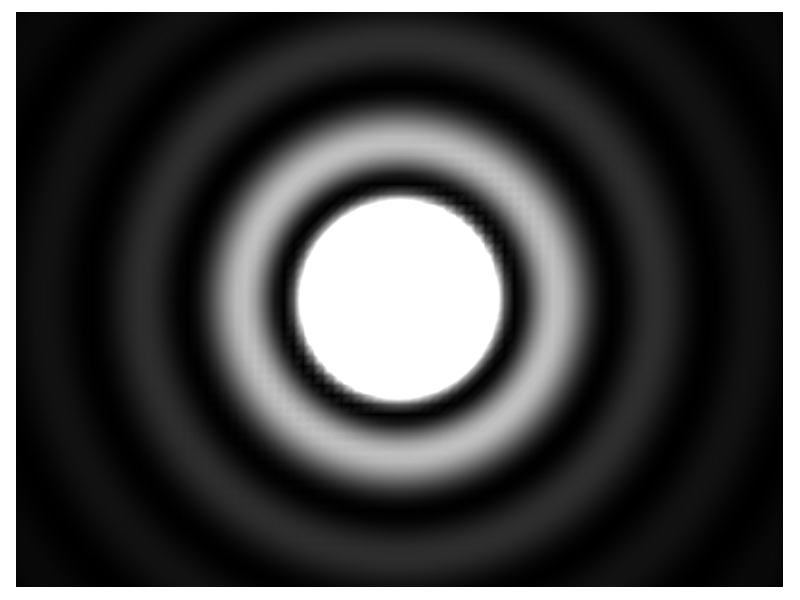
\includegraphics[width=4.7cm]{eiry-disk-0}\hfill
		\begin{tikzpicture}
			\begin{axis}[
				height	=	4.125cm,
				width	=	5.5cm,
				xlabel	=	{$x$, $\frac{\lambda}{D}$},
				ylabel	=	{$I/I_0$},
				ylabel shift	= -1 cm,
				]
				
				\addplot[smooth] table[x=x, y=e0]{data/eiry-disk-profile.txt};
			\end{axis}
		\end{tikzpicture}
		\caption{Диффракционное изображение от одного источника}
	\end{subfigure}\\
	\begin{subfigure}[t]{\tw}
		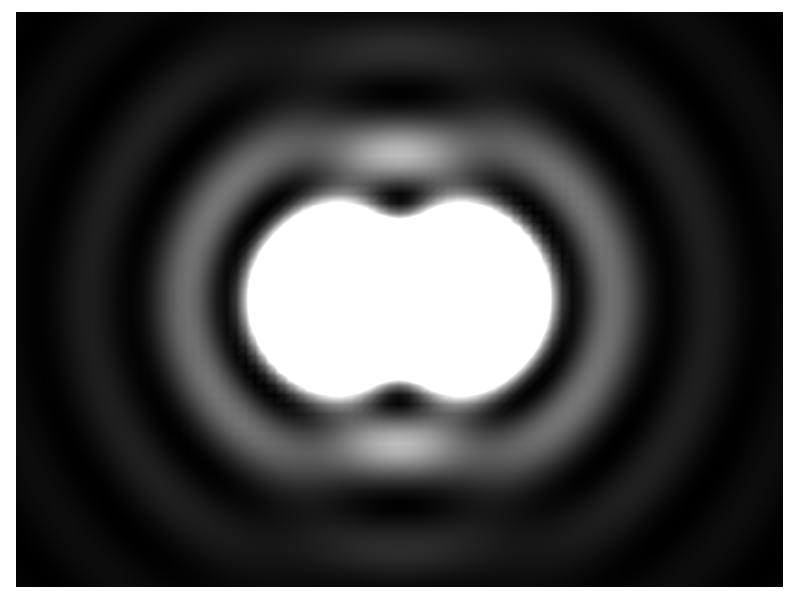
\includegraphics[width=4.7cm]{eiry-disk-1}\hfill
		\begin{tikzpicture}
			\begin{axis}[
				height	=	4.125cm,
				width	=	5.5cm,
				xlabel	=	{$x$, $\frac{\lambda}{D}$},
				ylabel	=	{$I/I_0$},
				ylabel shift	= -1 cm,
				]
				
				\addplot[smooth] table[x=x, y=e1]{data/eiry-disk-profile.txt};
			\end{axis}
		\end{tikzpicture}
		\caption{Диффракционное изображение от двух источников с разделением~$1.22\lambda/D$}
	\end{subfigure}\\
	\begin{subfigure}{\tw}
		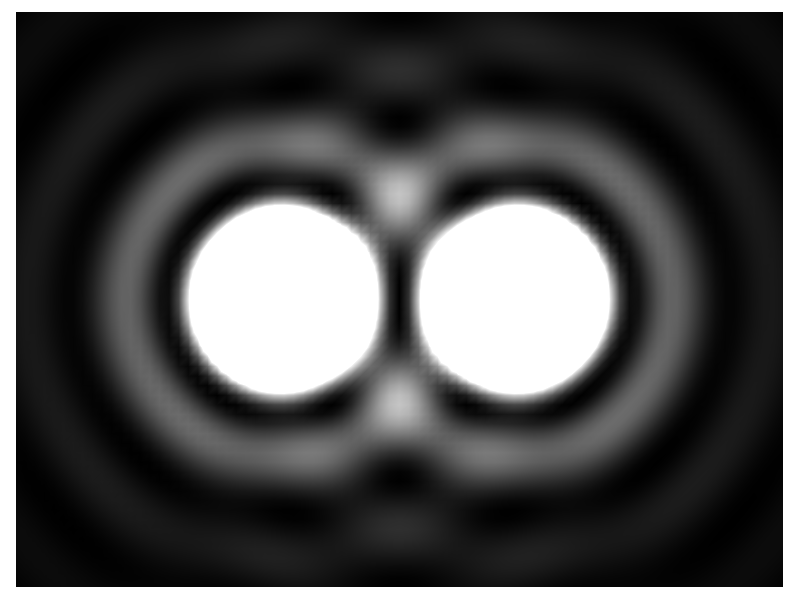
\includegraphics[width=4.7cm]{eiry-disk-2}\hfill
		\begin{tikzpicture}
			\begin{axis}[
				height	=	4.125cm,
				width	=	5.5cm,
				xlabel	=	{$x$, $\frac{\lambda}{D}$},
				ylabel	=	{$I/I_0$},
				ylabel shift	= -1 cm,
				]
				
				\addplot[smooth] table[x=x, y=e2]{data/eiry-disk-profile.txt};
			\end{axis}
		\end{tikzpicture}
		\caption{Диффракционное изображение от двух источников с разделением~$2 \cdot 1.22\lambda/D$}
	\end{subfigure}\\
	\begin{subfigure}{\tw}
		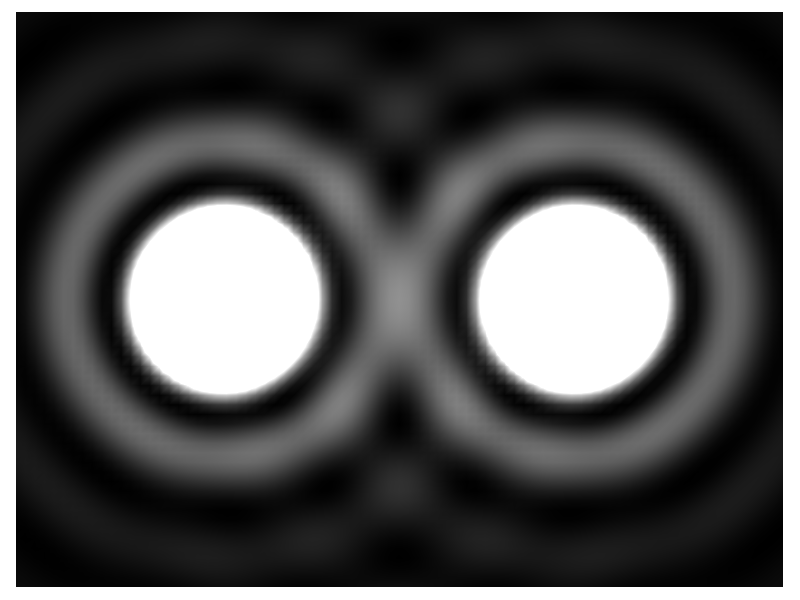
\includegraphics[width=4.7cm]{eiry-disk-3}\hfill
		\begin{tikzpicture}
			\begin{axis}[
				height	=	4.125cm,
				width	=	5.5cm,
				xlabel	=	{$x$, $\frac{\lambda}{D}$},
				ylabel	=	{$I/I_0$},
				ylabel shift	= -1 cm,
				]
				
				\addplot[smooth] table[x=x, y=e3]{data/eiry-disk-profile.txt};
			\end{axis}
		\end{tikzpicture}
		\caption{Диффракционное изображение от двух источников с разделением~$3 \cdot 1.22\lambda/D$}
	\end{subfigure}
	\caption{}
\end{figure}




	\section{Сферическая астрономия}
\subsection{Системы небесных координат}
Каждая из систем небесных координат является сферической системой координат, в которой радиус не имеет значения, так как параллакс не учитывается, а объекты считаются бесконечно удалёнными от наблюдателя.

\begin{figure}[!h]
	\centering
	\begin{subcaptionblock}{0.49\textwidth}
		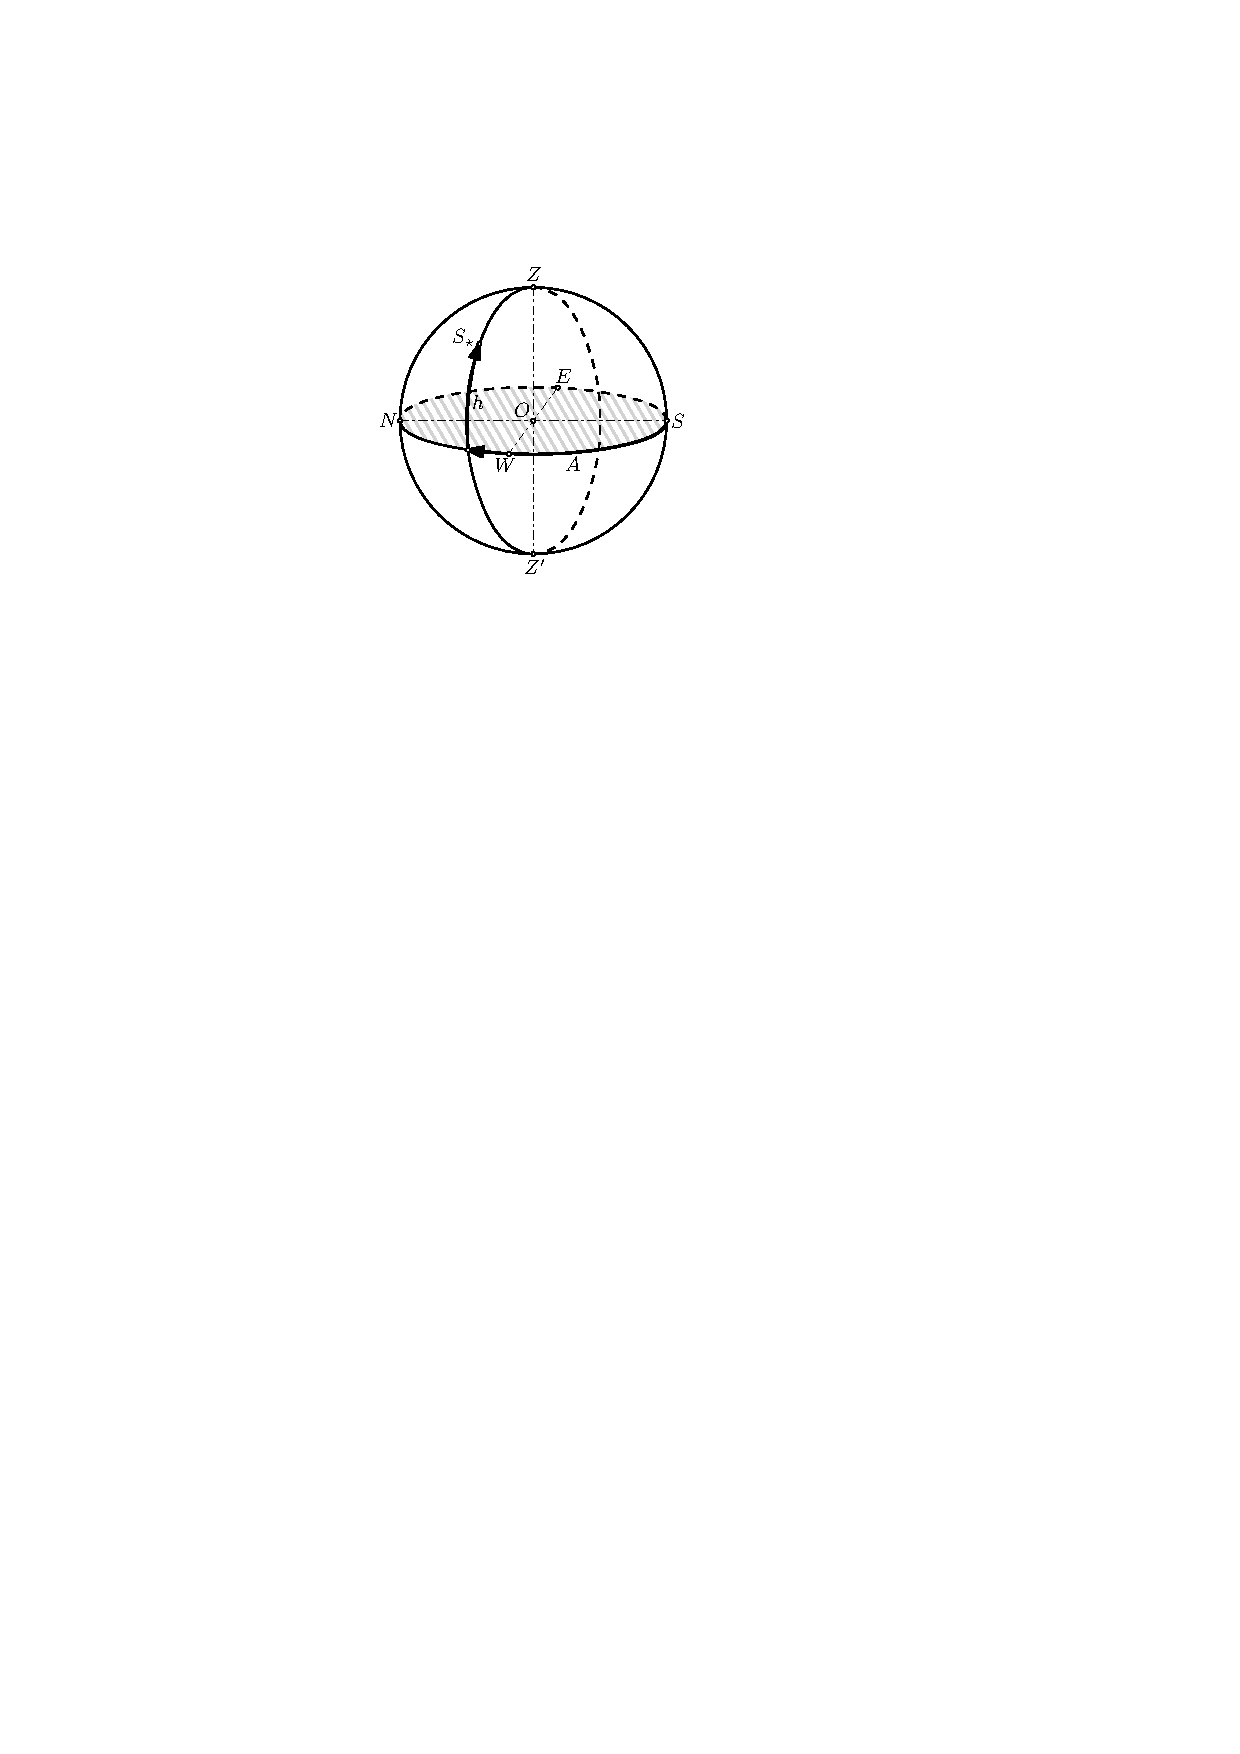
\includegraphics[width = \textwidth]{hor-coordin-sys}
		\caption{Горизонтальная система координат}
	\end{subcaptionblock}
	\hfill
	\begin{subcaptionblock}{0.49\textwidth}
		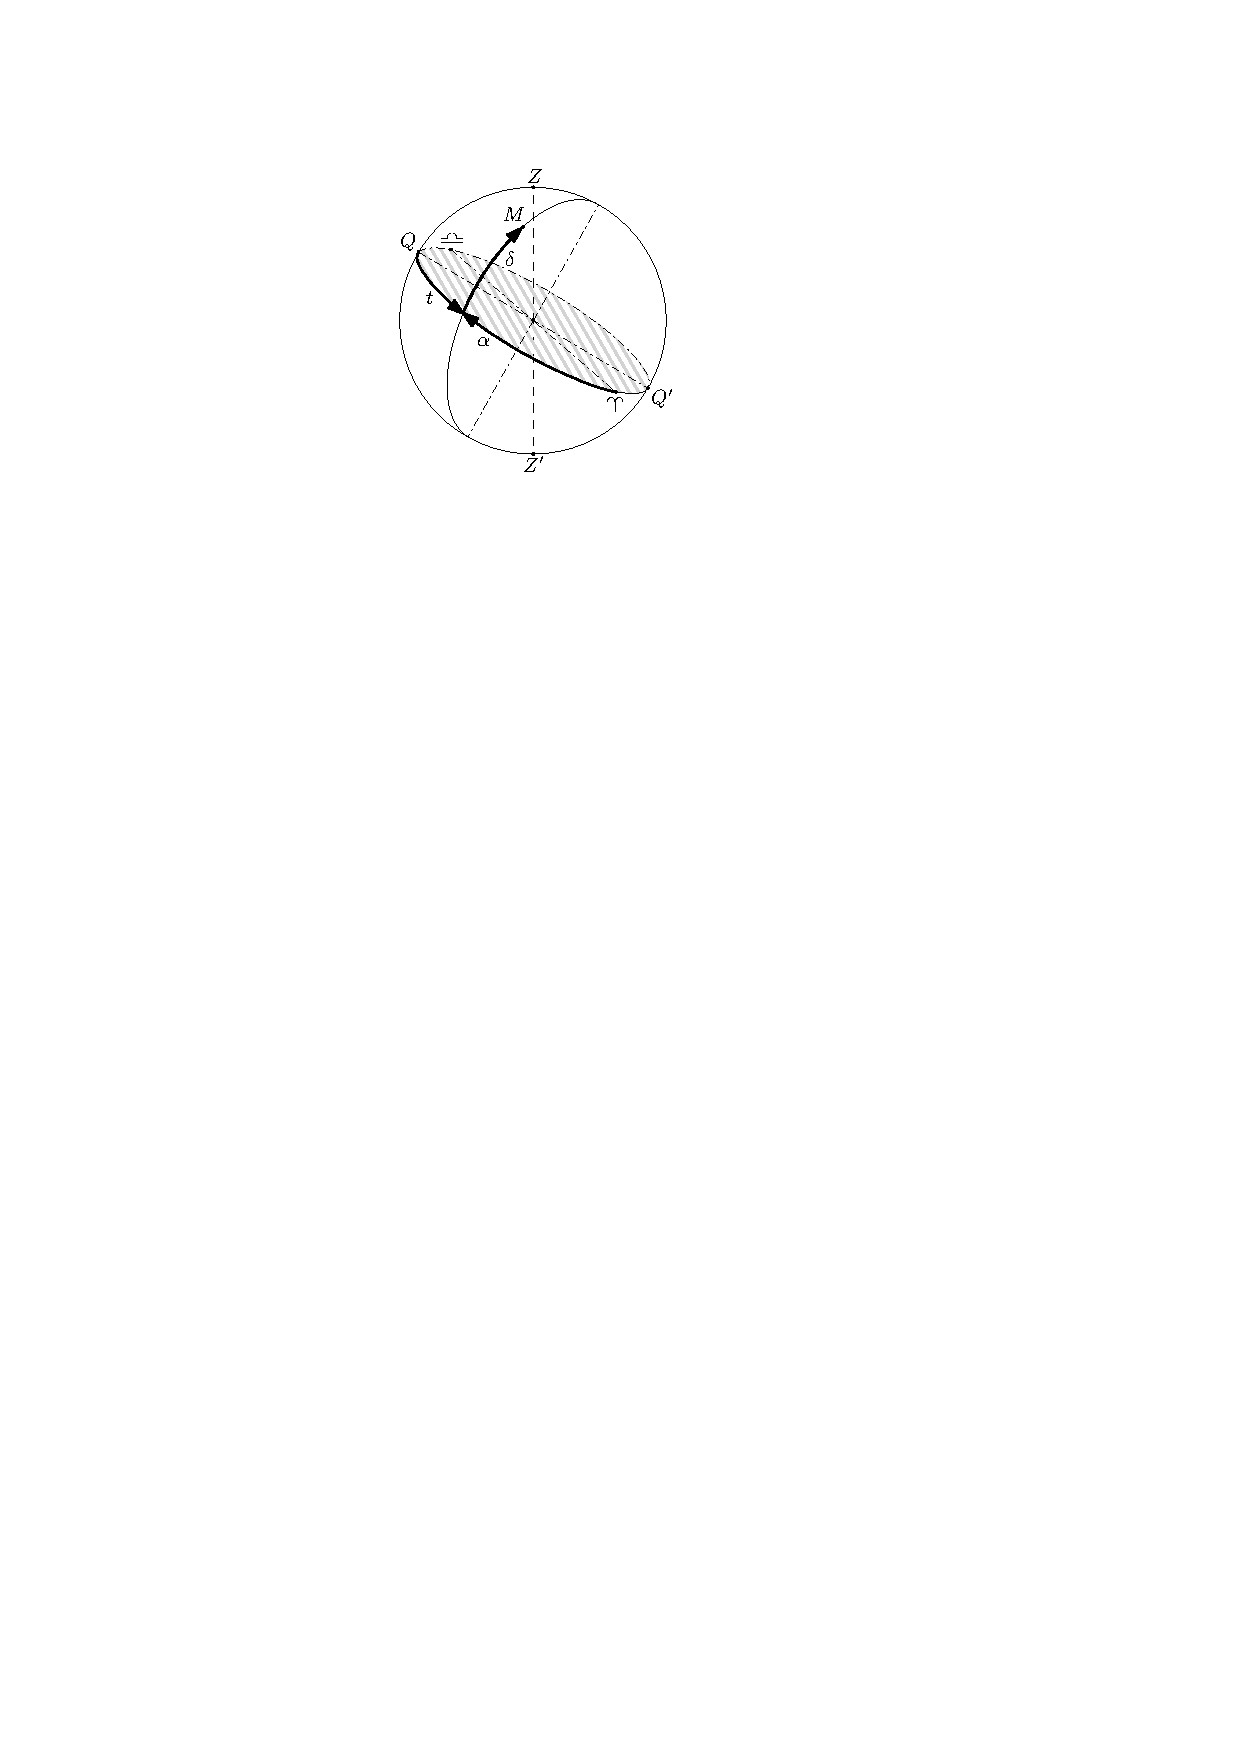
\includegraphics[width = \textwidth]{eq-coordin-sys}
		\caption{Экваториальная система координат}
	\end{subcaptionblock}
	\caption{Системы координат I}
\end{figure}
\term{Горизонтальная система координат}~--- система координат, в которой основной плоскостью является плоскость математического горизонта, а полюсами~--- \term{зенит} и \term{надир}~--- точки небесной сферы, расположенные ровно над наблюдателем и под ним соответственно. Одной координатой является либо \term{высота} светила $h$~--- угловое расстояние между светилом и математическим горизонтом, отсчитываемое в сторону зенита, либо его \term{зенитное расстояние}~$z$~--- угловое расстояние между зенитом и светилом. Другой координатой является \term{астрономический азимут} $A$~--- угол $SZS_\star$, отсчитываемый в сторону запада. Половина большого круга, перпендикулярного горизонту,~--- $Z S_\star Z'$  называется \term{вертикалом} объекта.

\term[экваториальная система координат]{Первая экваториальная система координат}~--- система координат,
основной плоскостью которой является плоскость небесного экватора $QEQW'$.
Одной координатой при этом является \term{склонение}~$\delta$~--- угловое
расстояние между светилом и плоскостью небесного экватора, отсчитываемое в
сторону севера. Половина большого круга, вдоль которой отсчитывается склонение,
перпендикулярна небесному экватору и называется \term[круг склонений]{кругом склонений} или
\imp{кругом равных часовых углов (прямых восхождений)}. Наряду со склонением
используется \term{полярное расстояние}~$p$~--- угловое расстояние между
светилом и полюсом мира. Другой координатой является \term{часовой угол}~$t$~---
дуга небесного экватора от верхней точки небесного экватора до круга склонения
светила в сторону запада, или угол между небесным меридианом и кругом склонения
светила. $\aries$ и $\libra$~--- точки весеннего и осеннего равноденствия соответственно.

\term[экваториальная система координат]{Вторая экваториальная система координат}~--- система, аналогичная предыдущей. Одной координатой по прежнему является \term{склонение}~$\delta$. А другой координатой является \term{прямое восхождение}~$\alpha$~--- угловое расстояние между точкой весеннего равноденствия и кругом склонений светила в сторону годичного движения Солнца.

\begin{figure}[!h]
	\centering
	\begin{subcaptionblock}{0.49\textwidth}
		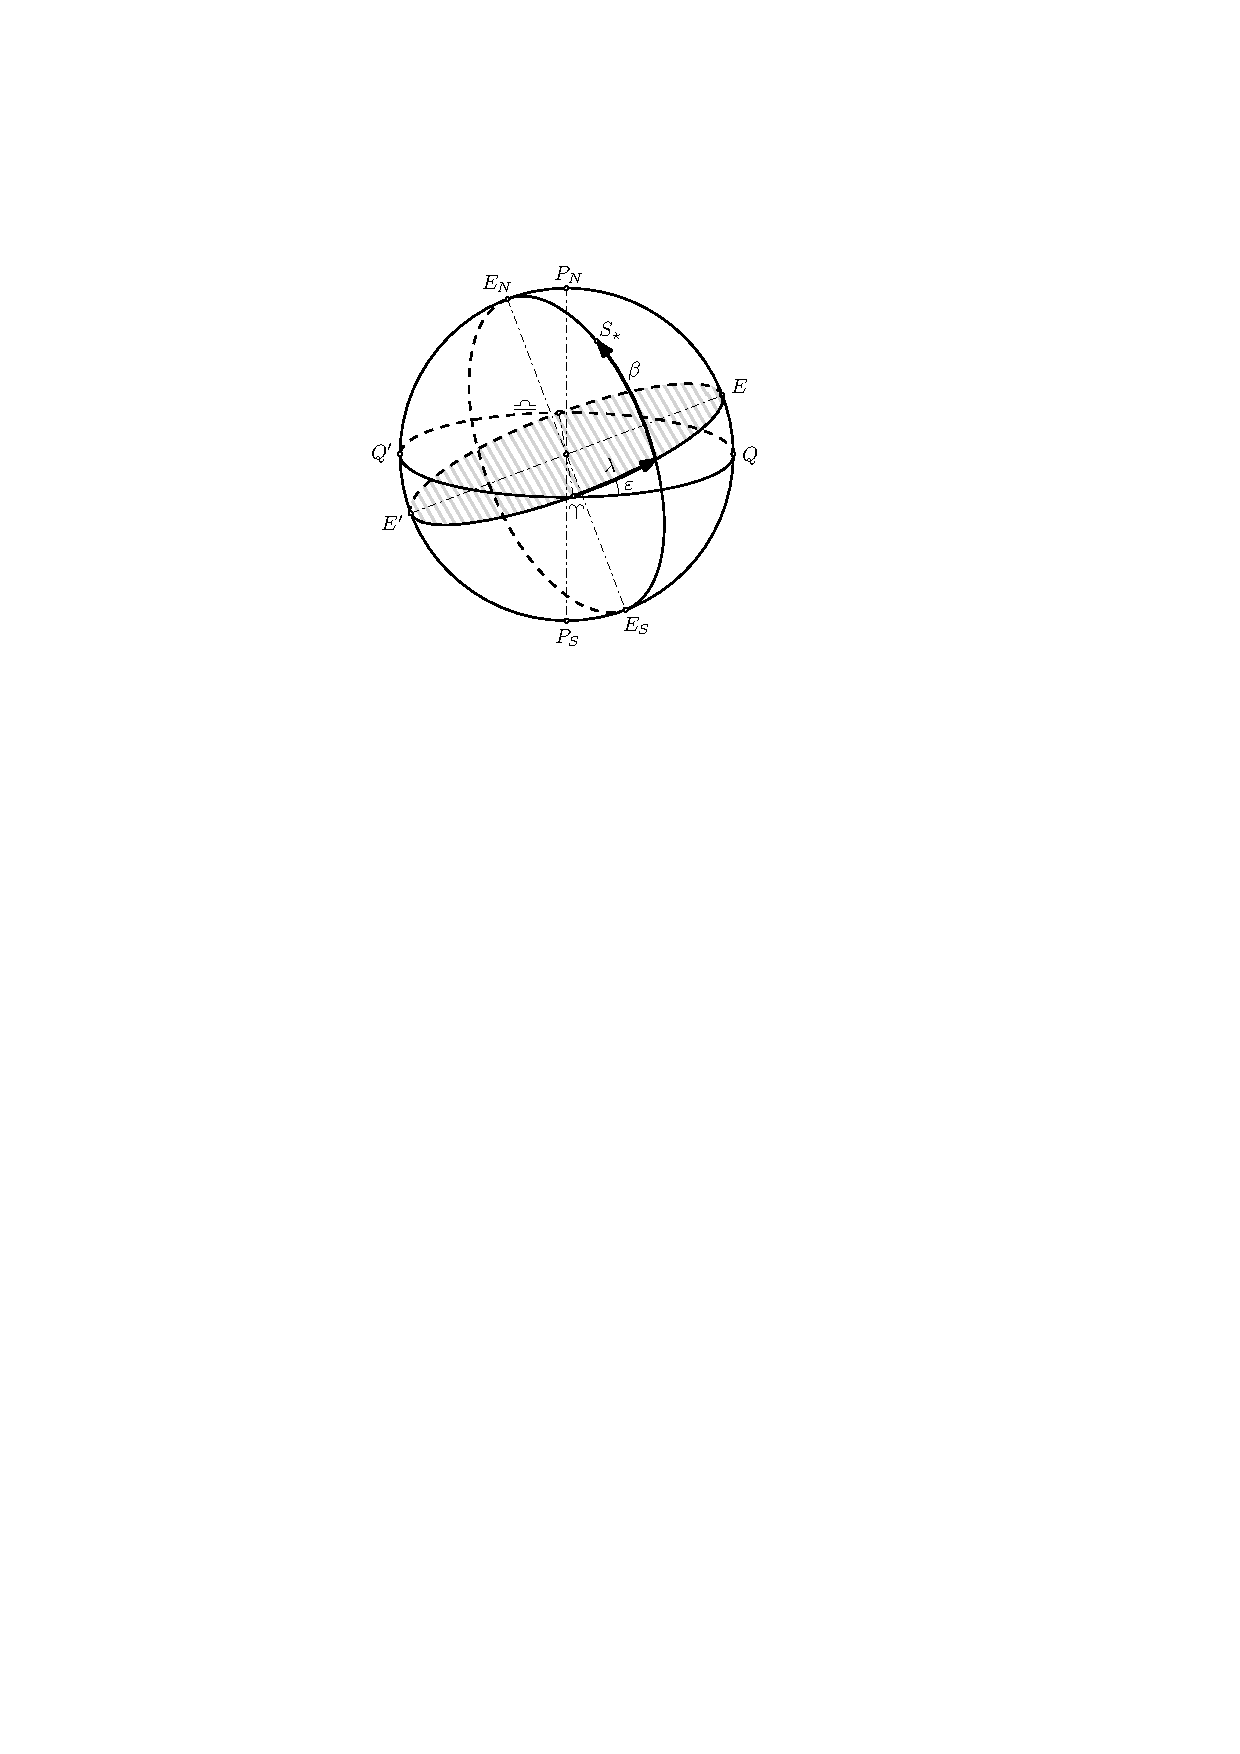
\includegraphics[width = \textwidth]{eql-coordin-sys}
		\caption{Эклиптическая система координат}
	\end{subcaptionblock}
	\hfill
	\begin{subcaptionblock}{0.49\textwidth}
		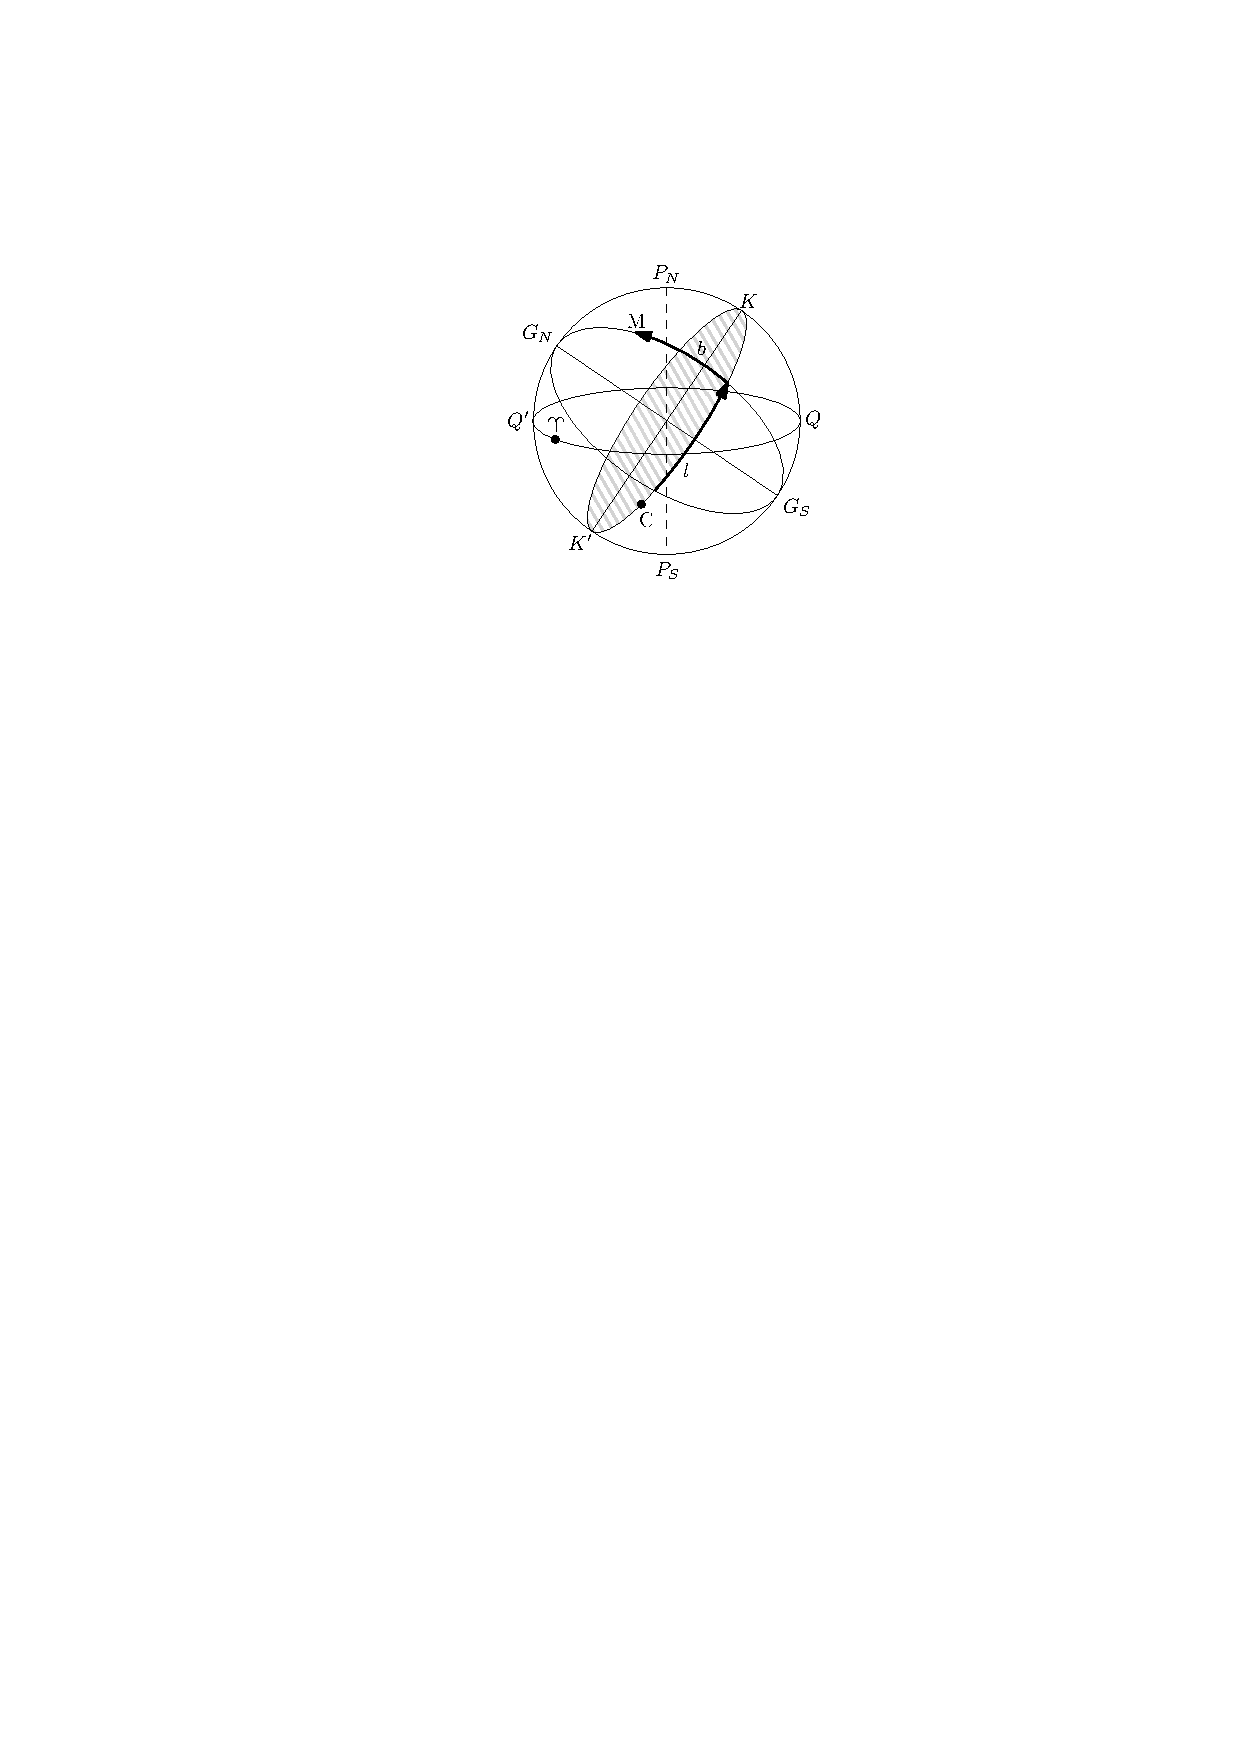
\includegraphics[width = \textwidth]{gal-coordin-sys}
		\caption{Галактическая система координат}
	\end{subcaptionblock}
	\caption{Системы координат II}
\end{figure}
\term{Эклиптическая система координат}~--- система координат, основной плоскостью которой является плоскость эклиптики $E \libra E' \aries $. Одной координатой при этом является \term{эклиптическая широта}~$\beta$~--- угловое расстояние между светилом и плоскостью эклиптики, отсчитываемое в сторону северного полюса мира, а другой~--- \term{эклиптическая долгота}~$\lambda$~--- угловое расстояние между точкой весеннего равноденствия и кругом эклиптической широты светила. Полюса эклиптики $E_N$ и $E_S$ имеют координаты ($18^h$,~$90^\circ - \varepsilon$) и ($6^h$,~$-90^\circ + \varepsilon$).

\term{Галактическая система координат}~--- система координат, основной плоскостью которой является плоскость нашей галактики, которая наклонена к плоскости небесного экватора под углом $62.6^\circ$. Одной координатой при этом является \term{галактическая широта}~$b$~--- угол между плоскостью галактического экватора и направлением на светило, а другой~--- \term{галактическая долгота}~$l$~--- угол между направлением на точку начала отсчёта $C$ и плоскостью круга галактической широты светила. Точка $C$ является направлением на центр галактики и имеет координаты: $\alpha=17^h\,45.6^m$, $\delta=-28^{\circ}\,56.2'$. $C K K'$~--- плоскость галактического экватора; $G_N$, $G_S$~--- северный и южный полюса галактики соответственно.

\subsection{Суточное вращение небесной сферы}
Вследствие вращения Земли вокруг своей оси для наблюдателя на поверхности небесные объекты совершают суточное движение параллельно небесному экватору, плоскость которого совпадает с плоскостью экватора Земли. Очевидно, в ходе такого движения высота светил постоянно меняется и в некоторые моменты времени достигает своего максимального и минимального значения.

\term[верхняя кульминация]{Верхняя} и \term{нижняя кульминация}~--- моменты пересечения светилом небесного меридиана, причём при верхней кульминации светило имеет наибольшую высоту, а при нижней~--- наименьшую.

Высота светила в верхней и нижней кульминации со склонением $|\delta| < |\varphi|$, соответственно:
\begin{equation}
	h_{\text{в}}= 90^\circ - \varphi + \delta, \quad\quad
	h_{\text{н}}= - 90^\circ + \varphi  + \delta.
\end{equation}

Если же светило имеет склонение $|\delta| > |\varphi|$, то высота в верхней и нижней кульминации вычисляется так:
\begin{equation}
	h_{\text{в}}= 90^\circ + \varphi - \delta, \quad\quad
	h_{\text{н}}= - 90^\circ -\varphi - \delta.
\end{equation}

Из формул для высоты в нижней кульминации вытекает условие, определяющее, пересекает ли звезда горизонт:
\begin{equation}
	\begin{cases}
		h_\text{в} = +90^\circ - |\varphi - \delta| > 0^\circ,\\
		h_\text{н} = - 90^\circ + |\varphi + \delta| < 0^\circ;
	\end{cases}
	\quad \Longleftrightarrow \quad~~ |\delta|< 90^{\circ} - |\varphi|.
\end{equation}

Используя формулы сферической тригонометрии (см.\,\ref{sec:spher-trig}), можно выразить зависимость часового угла светила от его зенитного расстояния:
\begin{equation}
	\cos t=\frac{\cos z-\sin\varphi\sin\delta}{\cos\varphi\cos\delta}.
\end{equation}
Отсюда следует, что для часового угла захода и восхода светила справедливо равенство:
\begin{equation}
	\cos t_{\uparrow\downarrow}=-\tg\varphi\cdot\tg\delta.
\end{equation}

Аналогично, для вычисления азимута светила верна формула
\begin{equation}
	\cos A=\frac{\cos\delta\cos t-\cos\varphi\cos z}{\sin\varphi\sin z}.
\end{equation}
Следовательно, азимуты точек восхода и захода
\begin{equation}
	A_\uparrow = \arccos \left(-\dfrac{\sin\delta}{\cos \varphi} \right)\quad\text{и}\quad A_\downarrow = - A_\uparrow.
\end{equation}

\term{Звёздное время}~$z$~--- часовой угол точки весеннего равноденствия. Из определений прямого восхождения и часового угла следует справедливость равенства\begin{equation}
z = \alpha + t.
\end{equation}

\subsection{Сферическая тригонометрия}
\label{sec:spher-trig}
\begin{wrapfigure}[10]{r}{.3\tw}
    \centering
    \vspace{-1pc}
    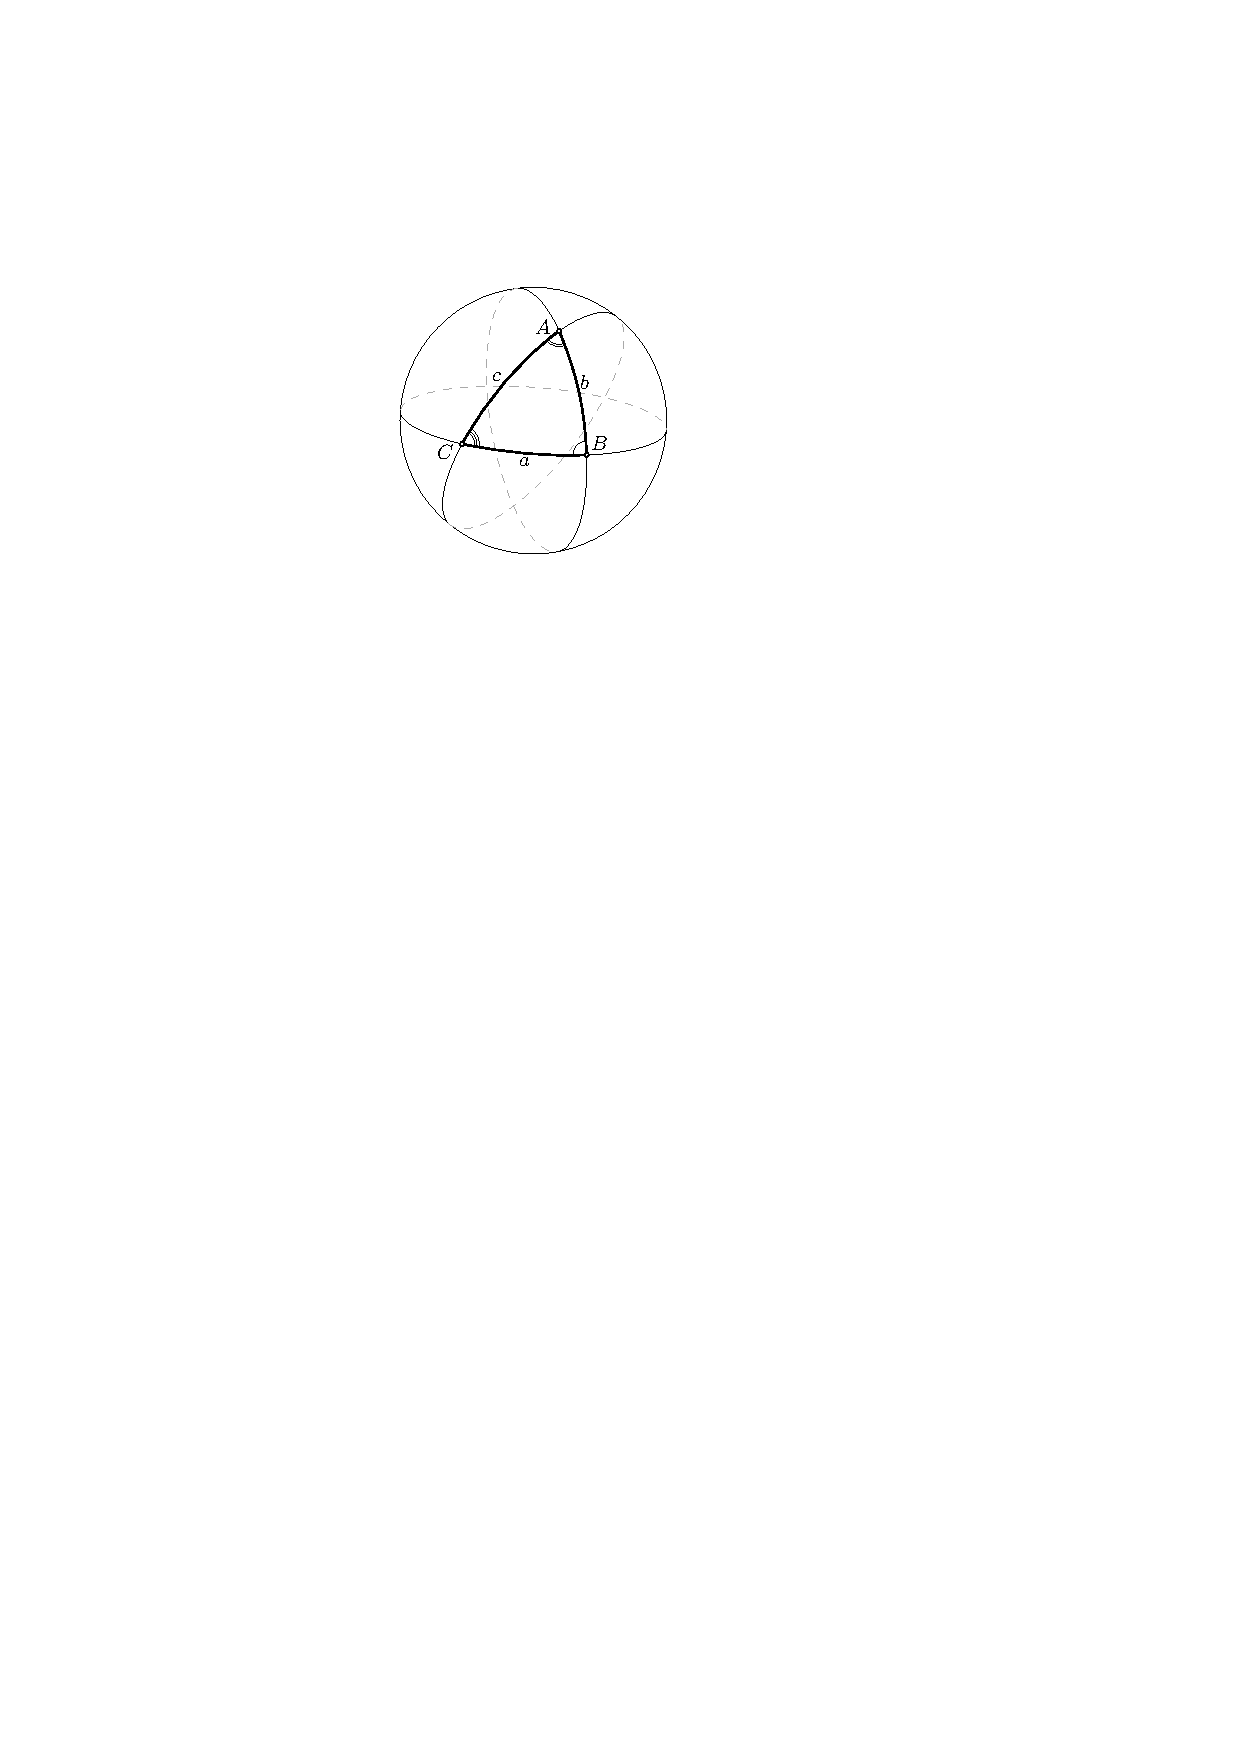
\includegraphics[width=0.3\textwidth]{spher-trigonom}
    \caption{Сферический треугольник}
\end{wrapfigure}
Для решения некоторых задач астрономии, связанных с видимыми положениями небесных тел, требуются знания о сферической тригонометрии. \imp{Сферический треугольник}~--- фигура на поверхности сферы, состоящая из трёх точек и трёх дуг больших кругов, соединяющих эти точки. Пусть $A$, $B$ и $C$~--- углы сферического треугольника, а $a$, $b$ и $c$~--- его стороны.

Сферические треугольники обладают следующими свойствами:
\begin{enumerate}
    \item Два сферических треугольника равны, если они подобны.
    \item Каждая сторона меньше суммы двух других сторон и больше их разности.
    \item Сумма всех сторон $a+b+c$ всегда меньше $2\pi$.
    \item Сумма углов сферического треугольника $\pi < A + B + C < 3\pi$.
    \item Разность суммы двух углов и третьего угла меньше $\pi$
\end{enumerate}

Площадь сферического треугольника определяется по формуле:
\begin{equation}
    S = R^2( A + B + C - \pi),
\end{equation}
где $A + B + C - \pi$~--- \imp{сферический избыток}.

Рассмотрим сферический треугольник $ABC$, радиус векторы вершин соответственно $\vec{a}$, $\vec{b}$ и $\vec{c}$.Причем из определения сферы $|\vec{a}| = |\vec{b}| = |\vec{c}| = r$. Пусть против вершин $A$, $B$ и $C$ лежат стороны с угловой мерой $a$, $b$ и $c$ соответсвенно. Повернем сферические координаты и нормируем так, чтобы $\vec{a} = (0, 0, 1)$, $\vec{b} = (\sin c, 0, \cos c)$, тогда $ \vec{c} = (\sin b \cos A, \sin b \sin A, \cos b)$.

Теперь запишем выражение для $\scalar{b}{c}$:
\begin{equation}
    \scalar{b}{c} = \cos a = \sin c \sin b \cos A + \cos c \cos b.
    \label{eq:spher-astro-cos-1}
\end{equation}
Аналогично,
\begin{gather}
    \scalar{a}{c} = \cos b = \sin a \sin c \cos B +  \cos a \cos c,\\
    \scalar{a}{b} = \cos c = \sin a \sin b \cos C + \cos a \cos b.
    \label{eq:spher-astro-cos-1-1}
\end{gather}
Выразим отсюда $\cos A$:
\begin{equation}
    \cos A = \frac{\cos a - \cos c \cos b}{\sin c \sin b}.
    \label{eq:spher-astro-cos-2}
\end{equation}
Формулы \eqref{eq:spher-astro-cos-1}\,--\,\eqref{eq:spher-astro-cos-2} называются \term{сферической теоремой косинусов} \imp{для стороны} \eqref{eq:spher-astro-cos-1}\,--\,\eqref{eq:spher-astro-cos-1-1} и, соответственно \imp{для угла} \eqref{eq:spher-astro-cos-2}.

Из основного тригонометрического тождества имеем:
\begin{multline*}
    \sin^2 A = 1 - \cos^2 A = 1 - \left[ \frac{\cos a - \cos c \cos b}{\sin c \sin b} \right]^2 = \\
    = \frac{\sin^2 c \sin^2 b - \cos^2 a + 2\cos a \cos c \cos b - \cos^2 c \cos^2 b}{\sin^2 c \sin^2 b}=\\
    = \frac{(1 - \cos^2 c)(1 -  \cos^2 b) - \cos^2 a + 2\cos a \cos c \cos b - \cos^2 c \cos^2 b}{\sin^2 c \sin^2 b}=\\
    = \frac{1 - \cos^2 c - \cos^2 b + \cos^2 c \cos^2 b -\cos^2 a}{\sin^2 c \sin^2 b} + \\
    + \frac{2\cos a \cos c \cos b - \cos^2 c \cos^2 b}{\sin^2 c \sin^2 b} = \\
    = \frac{1 - \cos^2 c - \cos^2 b - \cos^2 a + 2\cos a \cos c \cos b}{\sin^2 c \sin^2 b}.
\end{multline*}
Извлекая квадратный корень из левой и правой части и деля их на $\sin a$ имеем
\begin{equation*}
    \frac{\sin{A}}{\sin a} = \frac{\sqrt{1 - \cos^2 c - \cos^2 b - \cos^2 a + 2\cos a \cos c \cos b}}{\sin a \sin b \sin c}.
\end{equation*}
Заметим, что правая часть равенства циклична по переменным $a$, $b$ и $c$, следовательно, \term{сферическая теорема синусов} имеет вид
\begin{equation}
    \frac{\sin A}{\sin a} = \frac{\sin B}{\sin b} = \frac{\sin C}{\sin c}.
    \label{eq:sphere-th-sinus}
\end{equation}

Далее получим \term{формулу пяти элементов}. Для этого запишем теорему косинусов в выразим в ней один из косинусов, применяя ее же:
\begin{gather}
    \cos a = \sin c \sin b \cos A + \cos c \cos b,\nonumber\\
    \cos a = \sin c \sin b \cos A + \left( \sin a \sin b \cos C + \cos a \cos b \right)\cos b,\nonumber\\
    \cos a - \cos a \cos^2 b = \sin c \sin b \cos A + \sin a \sin b \cos b \cos C,\nonumber\\
    \cos a \sin^2 b = \sin c \sin b \cos A + \sin a \sin b \cos b \cos C,\nonumber\\
    \cos a \sin b = \sin a \cos b \cos C + \sin c \cos A.
    \label{eq:formula-5-elem}
\end{gather}


\begin{wrapfigure}[14]{r}{0.5\tw}
    \centering
    \vspace{-1pc}
    \tikzsetnextfilename{navigation-triangle}
    \tdplotsetmaincoords{70}{170}
    \begin{tikzpicture}[tdplot_main_coords]
        \footnotesize
        
        \def\r{2.5}
        \def\f{55}
        \def\d{20}
        \def\l{100}
        \def\t{60}


        % Draw spherical grid
        \draw[tdplot_screen_coords,thin,black!30] (0,0,0) circle (\r);
        \foreach \a in {-60,-30,...,60}{
            \tdplotCsDrawLatCircle[thin,black!20]{\r}{\a}
        }
        \foreach \a in {0,30,...,150}{
            \tdplotCsDrawLonCircle[thin,black!20]{\r}{\a}
        }
    
        
        % Delta coord of the intersection horizon and circle of equal right ascention
        \pgfmathsetmacro{\deltaMin}{atan(-cos(\t)/tan(\f))}
        
        % Angle between horizon and circle of equal right ascention
        \pgfmathsetmacro{\rotateAngle}{asin(cos(\t) * cos(\f) / sin(\deltaMin))}
        
        % 90 - Azimuth coord of the intersection horizon and circle of equal right ascention
        \pgfmathsetmacro{\AA}{acos(sin(\t) * cos(\deltaMin))}
        
        
        \pgfmathsetmacro\z{acos(sin(\f)*sin(\d) + cos(\f)*cos(\d)*cos(\t)}
        \pgfmathsetmacro\a{asin(cos(\d) * sin(\t) / sin(\z))}
        
    
        % Draw main azimuthal directions
        \draw [gray] (0,\r,0) -- (0,-\r,0);
        \draw [gray] (\r,0,0) -- (-\r,0,0);
        
        
        % Mark  and label angle A and 180 - A near Z
        \draw [double, fill=none, line cap=butt]({0.3*cos(180-\a - 3)},{0.3 * sin(180-\a -3)},\r) arc (180-\a-3:5:0.3);
        \tdplotCsLabelPoint{\r}{0}{0}{\adjustbox{right=10pt}{\scriptsize$180 \! - \!\!A$}}{below=3pt}
        
        
        % Mark and label angle t near P
        \def\angleRadius{0.4}
        \tdplotsetrotatedcoords{0}{-\f}{0};
        \draw [tdplot_rotated_coords, canvas is yz plane at x = \r]({\angleRadius * cos(80)},{\angleRadius * sin(80)}) arc (80:{90 - \t - 5}:\angleRadius);
        \tdplotCsLabelPoint{\r}{0}{90 - \f}{\adjustbox{raise=6pt}{$t$}}{right=9pt}
        
        
         % Mark right angles
        \tdplotsetrotatedcoords{0}{0}{180 - \a};
        \draw [tdplot_rotated_coords](\r,0.2,0.2) coordinate (c) (\r,0.2,0) coordinate (a1) -- (c) (\r,0,0.2) coordinate (a2) -- (c) pic [angle radius=0.2cm] {right angle=a1--c--a2};
        
        \tdplotsetrotatedcoords{0}{90 - \f}{180 - \t};
        \draw [tdplot_rotated_coords](\r,0.2,0.2) coordinate (c) (\r,0.2,0) coordinate (a1) -- (c) (\r,0,0.2) coordinate (a2) -- (c) pic [angle radius=0.2cm] {right angle=a1--c--a2};
        
        
        % Draw triangle
        \tdplotsetrotatedcoords{-90}{-90}{0};
        \draw[tdplot_rotated_coords, thick] (\r,0,0) arc (0:{90 -  \f}:\r);
        \tdplotsetrotatedcoords{\AA}{\rotateAngle}{\deltaMin};
        \draw[tdplot_rotated_coords, thick] (\r,0,0) arc (0:{90 - \d}:\r);
        \tdplotsetrotatedcoords{90 - \a}{-90}{0};
        \draw[tdplot_rotated_coords, thick] (\r,0,0) arc (0:\z:\r);
        
        
        %%%% Draw great circles
        % Celestial equator
        \tdplotCsDrawGreatCircle[semithick, tdplotCsFill/.style={opacity=0.0}]{\r}{0}{90 - \f}
        % Circle of equal azimuths
        \tdplotCsDrawGreatCircle[tdplotCsFill/.style={opacity=0.0}]{\r}{90 -\a}{90}
        % Celestial meridial
        \tdplotCsDrawGreatCircle[tdplotCsFill/.style={opacity=0.0}]{\r}{90}{90}
        % Circle of equal right ascension
        \tdplotCsDrawGreatCircle[tdplotCsFill/.style={opacity=0.0}]{\r}{180 + \AA}{180 - \rotateAngle}
        % Horizon
        \tdplotCsDrawLatCircle[semithick,tdplotCsFill/.style={opacity=0.00}]{\r}{0}

        
        % Draw and label points
        \tdplotCsDrawPoint{\r}{0}{90}
        \tdplotCsLabelPoint{\r}{0}{90}{$N$}{left}
        
        \tdplotCsDrawPoint{\r}{90}{90}
        \tdplotCsLabelPoint{\r}{90}{90}{$W$}{below right=-2pt}
        
        \tdplotCsDrawPoint{\r}{180}{90}
        \tdplotCsLabelPoint{\r}{180}{90}{$S$}{right}
        
        \tdplotCsDrawPoint{\r}{270}{90}
        \tdplotCsLabelPoint{\r}{270}{90}{$E$}{above}
        
        \tdplotCsDrawPoint{\r}{0}{0}
        \tdplotCsLabelPoint{\r}{0}{0}{$Z$}{above}
        
        \tdplotCsDrawPoint{\r}{0}{90 - \f}
        \tdplotCsLabelPoint{\r}{0}{90 - \f}{$P$}{above}
        
        \tdplotCsLabelPoint{\r}{90 + \a / 2}{88}{$A$}{above right = 3pt}
        
        
        % Label arcs
        \tdplotCsLabelPoint{\r}{0}{45 - \f / 2}{\adjustbox{right=12pt}{$90 - \varphi$}}{above}
        \tdplotCsLabelPoint{\r}{135 - \a / 2}{\z / 2}{$z$}{right=5pt}
        \tdplotCsLabelPoint{\r}{90 - \a / 2}{(90 - \f + \z) / 2}{\adjustbox{left=15pt}{$90 - \delta$}}{below=-13pt}
        \tdplotCsLabelPoint{\r}{180 - \t / 1.5}{45 + \f / 3}{$t$}{right}
        \tdplotCsLabelPoint{\r}{180 - \a + 6}{\z + (90 - \z) / 5}{$\delta$}{right}
        \tdplotCsLabelPoint{\r}{180 - \a}{\z + (90 - \z) / 2}{$h$}{left=-1pt}
        
        
        % Draw intersection oof celestial equator and celestial meridian
        \tdplotCsDrawPoint{\r}{180}{\f}
        
        % Draw star's projection on horizon
        \tdplotCsDrawPoint{\r}{180-\a}{90}
        
        % Draw star's projection on celestial equator
        \pgfmathsetmacro{\zz}{acos(cos(\f)*cos(\t)}
        \pgfmathsetmacro{\aa}{180 - asin(sin(\t) / sin(\zz))}
        \tdplotCsDrawPoint{\r}{\aa}{\zz}
        
        % Draw star
        \draw ({\r * cos(180 - \a) * sin(\z)}, {\r * sin(180 - \a) * sin(\z)}, {\r * cos(\z)}) node[star, star points=5, star point ratio=2.25, fill=black, scale=0.35] {};
        
        % Draw the center of sphere
        \tdplotCsDrawPoint{0}{0}{0}
    \end{tikzpicture}

    \caption{Параллактический треугольник}
    \label{pic:paralactic-triangle}    
\end{wrapfigure}

\term{Параллактический треугольник}~--- треугольник на небесной сфере, образованный пересечением небесного меридиана, вертикального круга и часового круга светила. \imp{Вертикальный круг}~--- большой круг небесной сферы, проходящий через надир, зенит и светило. \imp{Часовой круг}~--- большой круг небесной сферы, проходящий через полюса мира и наблюдаемое светило.

Применяя теоремы синусов и косинусов к параллактическому треугольнику, нетрудно получить следующие соотношения:
\begin{gather}
    \cos z=\sin\varphi\sin\delta+\cos\varphi\cos\delta\cos t\\
    \sin z\sin A=\cos\delta\sin t\\
    \sin z\cos A=-\cos\varphi\sin\delta+\sin\varphi\cos\delta\cos t
\end{gather}

\begin{wrapfigure}[11]{r}{0.42\tw}
    \centering
    \vspace{-1.5pc}
    \tikzsetnextfilename{grand-circle-eq}
    \tdplotsetmaincoords{70}{155}
    \begin{tikzpicture}[tdplot_main_coords]
        \footnotesize

        \def\r{2}
        \def\i{25}
        \def\lo{70}
        \def\l{100}
        \def\f{atan(sin(\l - \lo) * tan(\i))}

        \def\x{asin(sin(\f) / sin(\i))}
        \def\q{atan(sin(\x) * tan(\i))}
        \def\y{asin(sin(\q) / sin(\i))}
        \def\w{asin(sin(\x) / sin(\y))}


        \draw[tdplot_screen_coords,thin,black!30] (0,0,0) circle (\r);
        \foreach \a in {-60,-30,...,60}{
            \tdplotCsDrawLatCircle[thin,black!30]{\r}{\a}
        }
        \foreach \a in {0,30,...,150}{
            \tdplotCsDrawLonCircle[thin,black!30]{\r}{\a}
        }

        \tdplotCsDrawLatCircle[thick,tdplotCsFill/.style={opacity=0.00}]{\r}{0}

        \tdplotCsDrawGreatCircle[thick,tdplotCsFill/.style={opacity=0.0}]{\r}{\lo-90}{\i}

        \tdplotsetrotatedcoords{\y - 90 + \lo}{180 - \w}{\q};
        \draw[tdplot_rotated_coords, line width=1pt] (0,\r,0) arc (90:180:\r);
        \draw[tdplot_rotated_coords, anchor=north] (0,\r,0) node {\adjustbox{right=4mm,raise=-1mm}{$G$}};

        \tdplotsetrotatedcoords{\l - 90}{90}{\f};
        \draw[tdplot_rotated_coords, line width=1pt] (0,\r,0) arc (90:{180 -\f}:\r);

        \tdplotsetrotatedcoords{-180+\lo}{90}{90 - \i};
        \draw[tdplot_rotated_coords, line width=1pt] (0,\r,0) arc (90:{90+\i}:\r);

        \coordinate (P) at ({\r*cos(\lo - 90)*sin(\i)}, {\r*sin(\lo - 90)*sin(\i)},{\r*cos(\i)});
        \coordinate (P') at ({-\r*cos(\lo - 90)*sin(\i)}, {-\r*sin(\lo - 90)*sin(\i)},{-\r*cos(\i)});
        \draw[semithick, gray, dash dot, line cap=round] (P) -- (P');

        \def\x{asin(0.5/\r)}
        \tdplotsetrotatedcoords{-90+\lo+\x}{0}{0};
        \draw[tdplot_rotated_coords] (0,\r,0) arc (0:\i:5mm);

        \def\x{asin(0.2/\r)}
        \tdplotsetrotatedcoords{0}{-90 + \x}{-90 - \q};
        \draw[tdplot_rotated_coords] (0,\r,0) arc (200:315:2mm);

        \tdplotCsDrawPoint{\r}{\l}{90 - \f}

        \tdplotCsDrawPoint{\r}{\lo}{90}
        \tdplotCsLabelPoint{\r}{\lo}{90}{\adjustbox{left=4mm}{$(\lambda_0,0)$}}{anchor=north}

        \tdplotCsDrawPoint{\r}{\lo-90}{\i}
        \tdplotCsLabelPoint{\r}{\lo-90}{\i}{\adjustbox{left=5mm}{$P'$}}{anchor=south}

        \tdplotCsLabelPoint{\r}{0}{0}{}{label={[below]250:$\Delta \lambda$}}

        \tdplotCsDrawPoint{\r}{0}{0}
        \tdplotCsLabelPoint{\r}{0}{0}{$P$}{anchor=south}

        \tdplotCsLabelPoint{\r}{\lo-90}{\i/2}{$i$}{anchor=south}
        \tdplotCsLabelPoint{\r}{\l}{(90 - \f)/2 - 5}{$90^\circ - \varphi$}{anchor=west}
        \tdplotCsLabelPoint{\r}{\l - (\l - \lo + 90) /3 + 5}{(90 - \f + \i)/2 - 10}{$90^\circ$}{}

        \tdplotCsDrawPoint{\r}{0}{90}{}
        \tdplotCsLabelPoint{\r}{0}{90}{\adjustbox{left=2.5mm}{$(0,0)$}}{anchor= south}

        \tdplotCsDrawPoint{0}{0}{0}
    \end{tikzpicture}
    \caption{Произвольная точка $(\lambda, \varphi)$ на большом круге с полюсом $P'$}
    \label{pic:grand-circle}
\end{wrapfigure}
Напоследок, используя сферическую теорему косинусов, получим \term{уравнение большого круга}. Пусть на сфере заданы сферические координаты $(\lambda, \varphi)$, где $\lambda$~--- угол проекции вектора на плоскость $Oxy$ с осью $Ox$, \lookSecRef{sec:coord-systems}, а $\varphi$~--- угол между вектором в плоскостью $Oxy$. Найдем уравнение большого круга с наклонением $i$, восходящий узел которого находится в точке $(\lambda_0, 0)$.

Для этого рассмотрим произвольную точку $G = (\lambda, \varphi)$ на этом большом круге и один из его полюсов $P' = (\lambda_0 - 90^\circ,\,90^\circ - i)$. По определению большого круга каждая его точка отстоит от полюса на $90^\circ$. Обозначим разность первых координат $P'$ и $G$~--- $\lambda - (\lambda_0 - 90^\circ)$, за $\Delta \lambda$ и запишем сферическую теорему косинусов для $\triangle PP'G$, где $P$~--- полюс заданной системы координат:
\begin{gather}
    \cos 90^\circ = \cos i \cos (90^\circ - \varphi) + \sin i \sin (90^\circ - \varphi) \cos \Delta \lambda,\nonumber \\
    0 = \cos i \sin \varphi - \sin i \cos \varphi \sin (\lambda - \lambda_0),\nonumber\\
    \frac{\tg \varphi}{\tg i} = \sin (\lambda - \lambda_0),
    \label{eq:great-circle-eq}
\end{gather}
полученное уравнение является \imp{уравнением большого круга}.

\subsection{Солнечное время. Уравнение времени}

\term{Истинные солнечные сутки}~--- промежуток времени между двумя последовательными одноимёнными кульминациями Солнца.

\term{Истинное солнечное время}~--- промежуток времени между нижней кульминацией Солнца и его текущим положением. Рассчитывается по формуле
\begin{equation}
    T_{\text{ист}} = t_{\text{сол}}+12^h,
\end{equation}
где $t_{\text{сол}}$~--- часовой угол Солнца.

\term{Среднее Солнце}~--- точка небесной сферы, которая равномерно движется по небесному экватору с угловой скоростью, равной средней скорости изменения прямого восхождения Солнца.

\term{Среднее солнечное время} ($T_\text{ср}$)~--- время, прошедшее с последней нижней кульминации \imp{среднего Солнца}. Зная долготу наблюдателя, нетрудно вычислить среднее солнечное время:
\begin{equation*}
    T_\text{ср} = \text{UTC} + \frac{\lambda}{15^\circ/\text{час}},
\end{equation*}
где UTC~--- \imp{всемирное время}~--- среднее солнечное время на нулевом меридиане (меридиан с долготой $\lambda = 0^\circ$).

\term{Поясное} или \term{гражданское время}~--- среднее солнечное время на срединном меридиане географического часового пояса. В России также установлено декретное время, которое на 1 час больше поясного.

\begin{wrapfigure}[12]{r}{0.55\tw}
    \centering
    \vspace{-0.7pc}
    \tikzsetnextfilename{time-eq}
    \begin{tikzpicture}
        \begin{axis}[
            width    =    6.5cm,
            height    =    4.7cm,
            xmax     =    365,
            xmin    =    0,
            ymax    =    20,
            ymin     =     -20,
            ylabel    =    {$\eta$, мин},
            xlabel     =     {$d$, сут}
        ]
            \addplot [domain=0:365.25, samples = 100, black, smooth]{-7.65 * sin(360*x/365.25) + 9.86 * sin(2 * ( 102.9 + 360*x/365.25 ))};
        \end{axis}
    \end{tikzpicture}
    \caption{График уравнения времени}
    \label{pic:time-eq}
\end{wrapfigure}
\term{Уравнение времени}~--- разница между истинным солнечным временем и средним солнечным временем, возникающая по причине неравномерности движения Земли по орбите и наклона земного экватора к плоскости эклиптики (см.~Рис.\,\ref{pic:time-eq}). 

Получим приближенное выражение для величины уравнения времени. Для этого вспомним величину эксцентриситета орбиты Земли $e_\oplus = 0.017 \ll 1$, и рассмотрим выражение
\begin{multline}
    \sin E
        = \sin(E - M + M) =\\
        = \underbrace{\sin (E - M)}_{\simeq E - M} \cos M + \underbrace{\cos(E - M)}_{\simeq 1} \sin M \simeq\\
        \simeq (E - M) \cos M + \sin M,
        \label{eq:sun-time-sinE}
\end{multline}
так как $E - M \sim e$. Применим метод последовательных приближений, чтобы получить зависимость $E(M)$. Используем уравнение Кеплера~\eqref{eq:kepler-eq} и полученное выражение для $\sin E$~\eqref{eq:sun-time-sinE} для первого приближения: 
\begin{equation*}
    E_1
        = M + e \sin E
        = M + e \big( (E - M) \cos M + \sin M \big)
        \simeq M + e \sin M.
\end{equation*}
Воспользуемся полученным приближением, чтобы точнее оценить $E$,
\begin{equation}
    E
        = M + e \big( (E_1 - M) \cos M + \sin M \big)
        = M + e \sin M + \frac{e^2}{2} \sin 2M.
    \label{eq:sun-time-E(M)}
\end{equation}

Теперь запишем первые три члена многочлена Тейлора формулы перехода от истинной аномалии к эксцентрической~\eqref{eq:kepler-eq-E-nu-2}:
\begin{equation*}
    \nu
        = 2 \arctg \left(\sqrt{\frac{1+e}{1-e}} \tg \frac{E}{2} \right)
        \simeq E + e \sin E + \frac{e^2}{4} \sin 2E.
\end{equation*}
Подставим сюда выражение~\eqref{eq:sun-time-E(M)} для $E(M)$ и воспользуемся формулой для разложения синуса суммы:
\begin{multline*}
    \nu
        \simeq M + e \sin M + \frac{e^2}{2} \sin 2M + \\
        + e \bigg( 
            \sin M \cdot \underbrace{\cos (e \sin M + \ldots)}_{\simeq 1} + 
            \cos M \cdot \underbrace{\sin ( e \sin M  + \ldots )}_{\simeq e \sin M} 
        \bigg) + \\
        + \frac{e^2}{4} \bigg( 
            \sin 2M \cdot \underbrace{\cos (2e \sin M + \ldots)}_{\simeq 1} + 
            \cos 2M \cdot \underbrace{\sin (2e \sin M + \ldots)}_{\ll 1,~\text{с уч-м коэф-та}}
        \bigg)  \simeq \\
        \simeq M + 2e \sin M + \frac{5e^2}{4} \sin 2M.
\end{multline*}

Обозначим как $\omega = 103^\circ$ эклиптическую долготу перицентра, тогда эклиптическая долгота Солнца $\lambda = \nu + \omega$.



Теперь запишем формулу тангенса половинного угла для $\tg \frac{\varepsilon}{2}$ и воспользуемся выражением~\eqref{eq:tgAlpha/tgLambda} для $\cos \varepsilon$:
\begin{gather*}
    \tg^2 \frac{\varepsilon}{2} = \frac{1 - \cos \varepsilon}{1 + \cos \varepsilon} \equiv y ,\\
    1 - \frac{\tg \alpha}{\tg \lambda} = y \cdot \left( 1 + \frac{\tg \alpha}{\tg \lambda} \right),\\
    \sin \lambda \cos \alpha - \cos \lambda \sin \alpha = y \cdot \left( \sin \lambda \cos \alpha + \cos \lambda \sin \alpha \right),\\
    \sin ( \lambda - \alpha ) = y \sin(\alpha + \lambda),\\
    \alpha = \lambda - \arcsin \left( y \sin( \alpha + \lambda) \right).
\end{gather*}
Отметим, при $\varepsilon = 0$ выполняется $\alpha = \lambda$. Следовательно, можно сделать нулевое приближение $\alpha_0 = \lambda$. Воспользуемся методом последовательных приближений для получения более точного выражения для $\alpha(\lambda, \varepsilon)$.
\begin{gather}
    \alpha_1 = \lambda - \arcsin \left( y \sin (\alpha_0 + \lambda)  \right) \overset{\varepsilon \ll 1}{\simeq} \lambda - y \sin 2 \lambda,\nonumber\\
    \alpha_2
        = \lambda - \arcsin \left( y \sin (\alpha_1 + \lambda) \right)
        \overset{\varepsilon \ll 1}{\simeq} \lambda - y \sin 2 \lambda + \frac{y^2}{2} \sin 4 \lambda. \label{eq:second-approx-alpha-lambda}.
\end{gather}

Используем~\eqref{eq:second-approx-alpha-lambda} для записи уравнения времени:
\begin{multline}
    \eta
        = t_\text{ист} - t_\text{ср}
        = \alpha_2 - (M + \omega) = \\
        = \lambda - y \sin 2 \lambda + \frac{y^2}{2} \sin 4 \lambda - M - \omega = \\
        = \nu - y \sin (2\nu + 2\omega)  + \frac{y^2}{2} \sin (4\nu + 4\omega)  - M \simeq \\
        \overset{\varepsilon \ll 1,\, e \ll 1}{\simeq} \!\!\underbracket[0.5pt]{~2e \sin M\,}_\text{эксц-т орб.} - \underbracket[0.5pt]{\tg^2 \frac{\varepsilon}{2} \sin (2M + 2\omega)}_\text{наклон орбиты}.
        \label{eq:time-eq-M}
\end{multline}
Подставим~в~\eqref{eq:time-eq-M} параметры орбиты Земли:
\begin{equation*}
    e = 0.0167,~\varepsilon = 23.44^\circ,~\omega = 102.9^\circ,
\end{equation*}
чтобы получить уравнение времени в минутах,~\lookPicRef{pic:time-eq}:
\begin{equation}
    \eta = t_\text{ист} - t_\text{ср} =  -7.65 \sin \frac{2\pi d}{P} + 9.86 \sin 2 \left( 1.80 + \frac{2\pi d}{P} \right)~\text{мин},
\end{equation}
где $P = T_\text{сид}$~--- сидерический год (здесь не учитываются поправки, связанные с прецессией Земной оси), а $d$~--- время от момента прохождения точки перицентра (в современную эпоху это происходит в период со 2 по 5 января).

\subsection{Годичное движение Солнца}

\begin{wrapfigure}[23]{r}{0.62\tw}
    \vspace{-1pc}
    \centering
    \tikzsetnextfilename{analemma}
    \begin{tikzpicture}
        \footnotesize
        \begin{axis}[
            width    =    7.27cm,
            height    =    10cm,
            xmax     =    20,
            xmin    =    -20,
            ymax    =    27.5,
            ymin     =     -27.5,
            xlabel    =    {$\eta$, мин},
            ylabel     =     {$\delta_\odot$, $~^\circ$}
        ]
            \addplot[smooth] table[x=eta, y=delta, col sep = comma] {data/analemma.csv};
            \addplot[only marks, mark = o,mark options={scale=0.4, black}] table[x=eta, y=delta, col sep = comma] {data/analemma-months.csv}; %
            \draw (axis cs:-4.31549,-22.7642) node[anchor=south west] {01.01};
            \draw (axis cs:-13.7937,-15.9581) node[anchor=north east] {01.02};
            \draw (axis cs:-12.2946,-5.49806) node[anchor=south east] {01.03};
            \draw (axis cs:-3.41919,5.51223) node[anchor=south east] {01.04};
            \draw (axis cs:3.16321,15.5839) node[anchor=west] {01.05};
            \draw (axis cs:1.62501,22.3907) node[anchor=south west] {01.06};
            \draw (axis cs:-4.38004,22.7234) node[anchor=south east] {01.07};
            \draw (axis cs:-5.9518,16.4302) node[anchor=east] {01.08};
            \draw (axis cs:1.35013,6.67371) node[anchor=south west] {01.09};
            \draw (axis cs:12.2793,-4.12177) node[anchor=south west] {01.10};
            \draw (axis cs:16.6081,-14.6495) node[anchor=east] {01.11};
            \draw (axis cs:9.1938,-22.1884) node[anchor=south east] {01.12};
%            \draw [-latex, gray] (axis cs:5,-5) .. controls (axis cs:18,-20) and (axis cs:-15,-20) .. (axis cs:-5,-5);
%            \draw [-latex, gray] (axis cs:1,15) .. controls (axis cs:5,24) and (axis cs:-8,23) .. (axis cs:-3,15);
        \end{axis}
    \end{tikzpicture}
    \caption{Аналемма}
    \label{fig:analemma}
\end{wrapfigure}
В течение сидерического года Земля совершает полный оборот вокруг Солнца. Вследствие этого Солнце движется относительно далёких звёзд для наблюдателя на Земле. Это движение совершается по большому кругу небесной сферы~---  \term{эклиптике}~--- проекции орбиты Земли на небесную сферу. 

Однако, в силу прецессии земной оси, период такого движения равен \term{тропическому году}, который короче сидерического года примерно на 20~мин~25~сек.

%\begin{wrapfigure}[12]{r}{0.5\tw}
%    \centering
%    \vspace{-.9pc}
%    \tikzsetnextfilename{sun-path}
%    \begin{tikzpicture}
%        \begin{axis}[
%            width    =    .5\tw,
%            height    =    4.5cm,
%            xlabel    =    {Прямое восхождение $\alpha^h$},
%            ylabel    =    {Склонение $\delta^{\circ}$},
%            extra y ticks    =    {23.44, -23.44},
%            ytick = {-20, -10, 0, 10, 20},
%            ymax    =    25,
%            ymin    =    -25,
%            xmax    =    24,
%            xmin    =    0,
%            xtick    =    {0, 4, 8, 12, 16, 20, 24},
%            x dir = reverse
%            ]
%            \addplot [domain=0:24, samples=100] {atan(sin(x*15)*tan(23.44))};
%        \end{axis}
%    \end{tikzpicture}
%    \caption{График зависимости склонения Солнца от его прямого восхождения}
%\end{wrapfigure}
В моменты, когда Солнце находится в \imp{точке весеннего равноденствия}~$\aries$  (20~марта, реже~21) его координаты: $\alpha=0^h$, $\delta=0^{\circ}$. Во время прохождения этой точки обе координаты Солнца растут. Так происходит до момента, пока Солнце не пройдет \imp{точку летнего солнцестояния} (21~июня, реже~20), координаты которой~--- $\alpha=6^h$ и $\delta=\varepsilon$. После этого склонение Солнца начинает убывать. В момент прохождения \imp{точки осеннего равноденствия}~$\libra$ (22~или 23~сентября), координаты Солнца составляют $\alpha=12^h$, $\delta=0^{\circ}$. После прохождения \imp{точки зимнего солнцестояния} с координатами $\alpha=18^h$, $\delta=-\varepsilon$ (22~или 21~декабря) склонение Солнца начинает увеличиваться.

\begin{wrapfigure}[5]{r}{0.4\tw}
    \centering
    \vspace{-1pc}
    \tikzsetnextfilename{sun-lambda-alpha}
    \tdplotsetmaincoords{70}{-70}
    \begin{tikzpicture}[tdplot_main_coords]
        \footnotesize

        \def\R{5}
        \def\EPS{23.5}
        \def\ALPHA{45}
        \def\LAMBDA{atan(tan(\ALPHA)/cos(\EPS))}
        \def\DELTA{asin(sin(\LAMBDA)*sin(\EPS))}

        % Draw triangle
        \tdplotsetrotatedcoords{0}{0}{0};
        \draw[tdplot_rotated_coords, semithick] (\R,0,0) arc (0:{\ALPHA}:\R);
        \tdplotsetrotatedcoords{90}{-\EPS}{-90};
        \draw[tdplot_rotated_coords, semithick] (\R,0,0) arc (0:\LAMBDA:\R);
        \tdplotsetrotatedcoords{90+\ALPHA}{-90}{-90};
        \draw[tdplot_rotated_coords, semithick] (\R,0,0) arc (0:\DELTA:\R);

        % Draw points
        \tdplotCsDrawPoint{\R}{180}{-90}
        \tdplotCsDrawPoint{\R}{180 + \ALPHA}{-90 + \DELTA}
        \tdplotCsDrawPoint{\R}{180 + \ALPHA}{-90}

        % Label arcs
        \tdplotCsLabelPoint{\R}{180 + \ALPHA / 2}{-90}{$\alpha$}{below}
        \tdplotCsLabelPoint{\R}{180 + \ALPHA / 2}{-90 + \DELTA / 2}{$\lambda$}{above right}
        \tdplotCsLabelPoint{\R}{180 + \ALPHA}{-90 + \DELTA / 2}{$\delta$}{left}

        % Mark right angle
        \tdplotsetrotatedcoords{\ALPHA}{0}{0};
        \draw [tdplot_rotated_coords](\R,-0.2,0.2) coordinate (c) (\R,0,0.2) coordinate (a1) -- (c) (\R,-0.2,0) coordinate (a2) -- (c) pic [angle radius=0.2cm] {right angle=a1--c--a2};

        % Mark and label angle t near P
        \def\angleRadius{0.6}
        \tdplotsetrotatedcoords{0}{0}{0};
        \draw [tdplot_rotated_coords, canvas is yz plane at x = \R]({\angleRadius * cos(\EPS)},0) arc (0:{\EPS - 3}:\angleRadius);
        \tdplotCsLabelPoint{\R}{6}{88.3}{$\varepsilon$}{left}
    \end{tikzpicture}
    \caption{}
    \label{pic:sun-lambda-alpha}
\end{wrapfigure}
Найдём выражение для прямого восхождения Солнца $\alpha$ через переменные $\lambda$ и $\varepsilon$, где $\varepsilon = 23.44^\circ$~--- угол наклона экватора Земли к эклиптике. Для этого рассмотрим формулу пяти элементов~\eqref{eq:formula-5-elem} для прямоугольного сферического треугольника, представленного на рисунке~\picRef{pic:sun-lambda-alpha}:
\begin{gather}
    \sin \delta \cos 90^\circ = \cos \lambda \sin \alpha - \sin \lambda \cos \alpha \cos \varepsilon,\notag\\
    \cos \lambda \sin \alpha = \sin \lambda \cos \alpha \cos \varepsilon,\notag\\
    \frac{\tg \alpha }{\tg \lambda} = \cos \varepsilon.
    \label{eq:tgAlpha/tgLambda}
\end{gather}

Из аналогичных рассуждений несложно получить, что прямое восхождение Солнца связано со склонением формулой. Рассмотрим формулу пяти элементов~\eqref{eq:formula-5-elem},
\begin{gather*}
    \cos \delta \sin \alpha = \sin \delta \cos \alpha \cos 90^\circ + \sin \lambda \cos \varepsilon,\\
    \cos \delta \sin \alpha = \sin \lambda \cos \varepsilon.
\end{gather*}
Выразим $\sin \lambda$ из теоремы синусов~\eqref{eq:sphere-th-sinus}:
\begin{equation*}    
    \sin \lambda = \frac{\sin \delta}{\sin \varepsilon}.
\end{equation*}
и подставим в полученное выше равенство:
\begin{equation}
    \sin\alpha = \frac{\tg\delta}{\tg\varepsilon}.  
    \label{eq:sin-alpha}
\end{equation}





\subsection{Рефракция}
\term{Рефракция}~--- явление преломления световых лучей, приходящих от небесных светил, в атмосфере планеты. Вследствие рефракции для наблюдателя на поверхности планеты с атмосферой видимая высота светила отличается от истинной на некоторый угол~--- \imp{величину рефракции}.

Для зенитного расстояния $z < 70^\circ$ величину рефракции можно определить по формуле
\begin{equation}
    \rho = 60.25'' \cdot \tg z' \cdot \frac{p}{760} \frac{273^{\circ}}{273^{\circ}+ t^{\circ}},
    \label{eq:refrac}
\end{equation}
где $t^{\circ}$~--- температура воздуха в градусах Цельсия, $p$~--- атмосферное давление в мм~рт.\,ст., $z'$~--- видимое зенитное расстояние. При н.\,у.: $p = 760$ мм~рт.\,ст. и $t = 0^{\circ}$C, формула \eqref{eq:refrac} принимает вид
\begin{equation}
    \rho = 60.25'' \cdot \tg z'.
\end{equation}

\begin{wrapfigure}{l}{0.35\tw}
    \centering
    \vspace{-1pc}
    \tikzsetnextfilename{refraction}
    \begin{tikzpicture}[scale=1]
        \footnotesize
        \coordinate (O) at (0, 0) {};

        \draw (2, 0) arc(0:110:2);
        \draw (3, 0) arc(0:105:3);

        \draw (0, .3) arc(90:41.8:.3);
        \draw [double, line cap=butt](1.94, 2) arc(180:221.8:.3);
        \draw [decoration={snake, segment length=1mm, amplitude=0.3mm}, decorate](2.52, 1.89) arc(-21.5:41.8:.3);
        \draw (0, 1.8) -- (.2, 1.8) -- (.2, 2);

        \draw (O) -- (0, 3);
        \draw (0,2) -- (2.24, 2) -- (3, 1.7);
        \draw [-latex] (0, 2) -- (1.24, 2);
        \draw [-latex] (2.24, 2) -- (2.848, 1.76);
        \draw [dashes] (O) -- (2.98, 2.67);

        \draw (O) node[anchor=north east] {$C$};
        \draw (0, 3) node[anchor=south east] {$Z$};
        \draw (0, 2) node[anchor=south east] {$O$};
        \draw (0, 1) node[anchor=east] {$R_\oplus$};
        \draw (0.75, 0.72) node[anchor=north west] {$R_\oplus$};
        \draw (1.85, 1.72) node[anchor=north west] {$h$};

        \draw (.17, .25) node[anchor=south] {$\alpha$};
        \draw (1.95, 2.05) node[anchor=north east] {$\beta$};
        \draw (2.55, 2.07) node[anchor= west] {$\beta'$};

        \draw [fill=white] (O) circle (.03);
        \draw [fill=white] (0, 2) circle (.03);
        \draw [fill=white] (0, 3) circle (.03);
    \end{tikzpicture}
    \caption{}
    \label{pic:refraction}
\end{wrapfigure}

Однако для расчета рефракции у горизонта данная формула не подходит. Получим оценку на величину рефракции у горизонта, считая атмосферу Земли однородной, положив её высоту $h$ равной 8~км. 

Рассмотрим луч зрения, лежащий в плоскости математического горизонта наблюдателя. Найдём угол между лучом и нормалью к верхней границе атмосферы в точке выхода луча из атмосферы (\lookPicRef{pic:refraction}):
\begin{equation*}
    \beta = 90^\circ - \alpha = 90^\circ - \arccos \frac{R_\oplus}{R_\oplus + h} = 87.13^\circ.
\end{equation*}
Для любой другой высоты атмосферы и радиуса планеты расчёт производится ровно также с соответствующими параметрами.

Коэффициент преломления воздуха $n_\text{в}$ при давлении $p = 1$~атм и температуре $t=0^\circ\text{C}$ равен $1 + 2.9\times 10^{-4}$. Следовательно угол преломления будет равен $\beta' = \arcsin n_\text{в} \sin \beta = 87.48^\circ$. Величина отклонения луча и есть рефракция, то есть $\rho = \beta' - \beta = 0.35^\circ$.

Реальное же значение рефракции $\rho_0$ у горизонта составляет около $0.5^\circ$.


\subsection{Сумерки}
\term{Сумерки}~--- часть суток, когда Солнце находится неглубоко под горизонтом.
В зависимости от высоты Солнца под горизонтом различают \imp{гражданские}, \imp{навигационные} и \imp{астрономические} сумерки:\\
\begin{minipage}{0.54\tw}
	\begin{enumerate}
		\item Гражданские~--- от $0^{\circ}$ до $-6^{\circ}$
		\item Навигационные~--- от $-6^{\circ}$ до $-12^{\circ}$
		\item Астрономические~--- от $-12^{\circ}$ до $-18^{\circ}$
	\end{enumerate}
	Когда Солнце опускается ниже $-18^{\circ}$, наступает ночь.
\end{minipage}
\hfill
\begin{minipage}{0.44\tw}
	\centering
	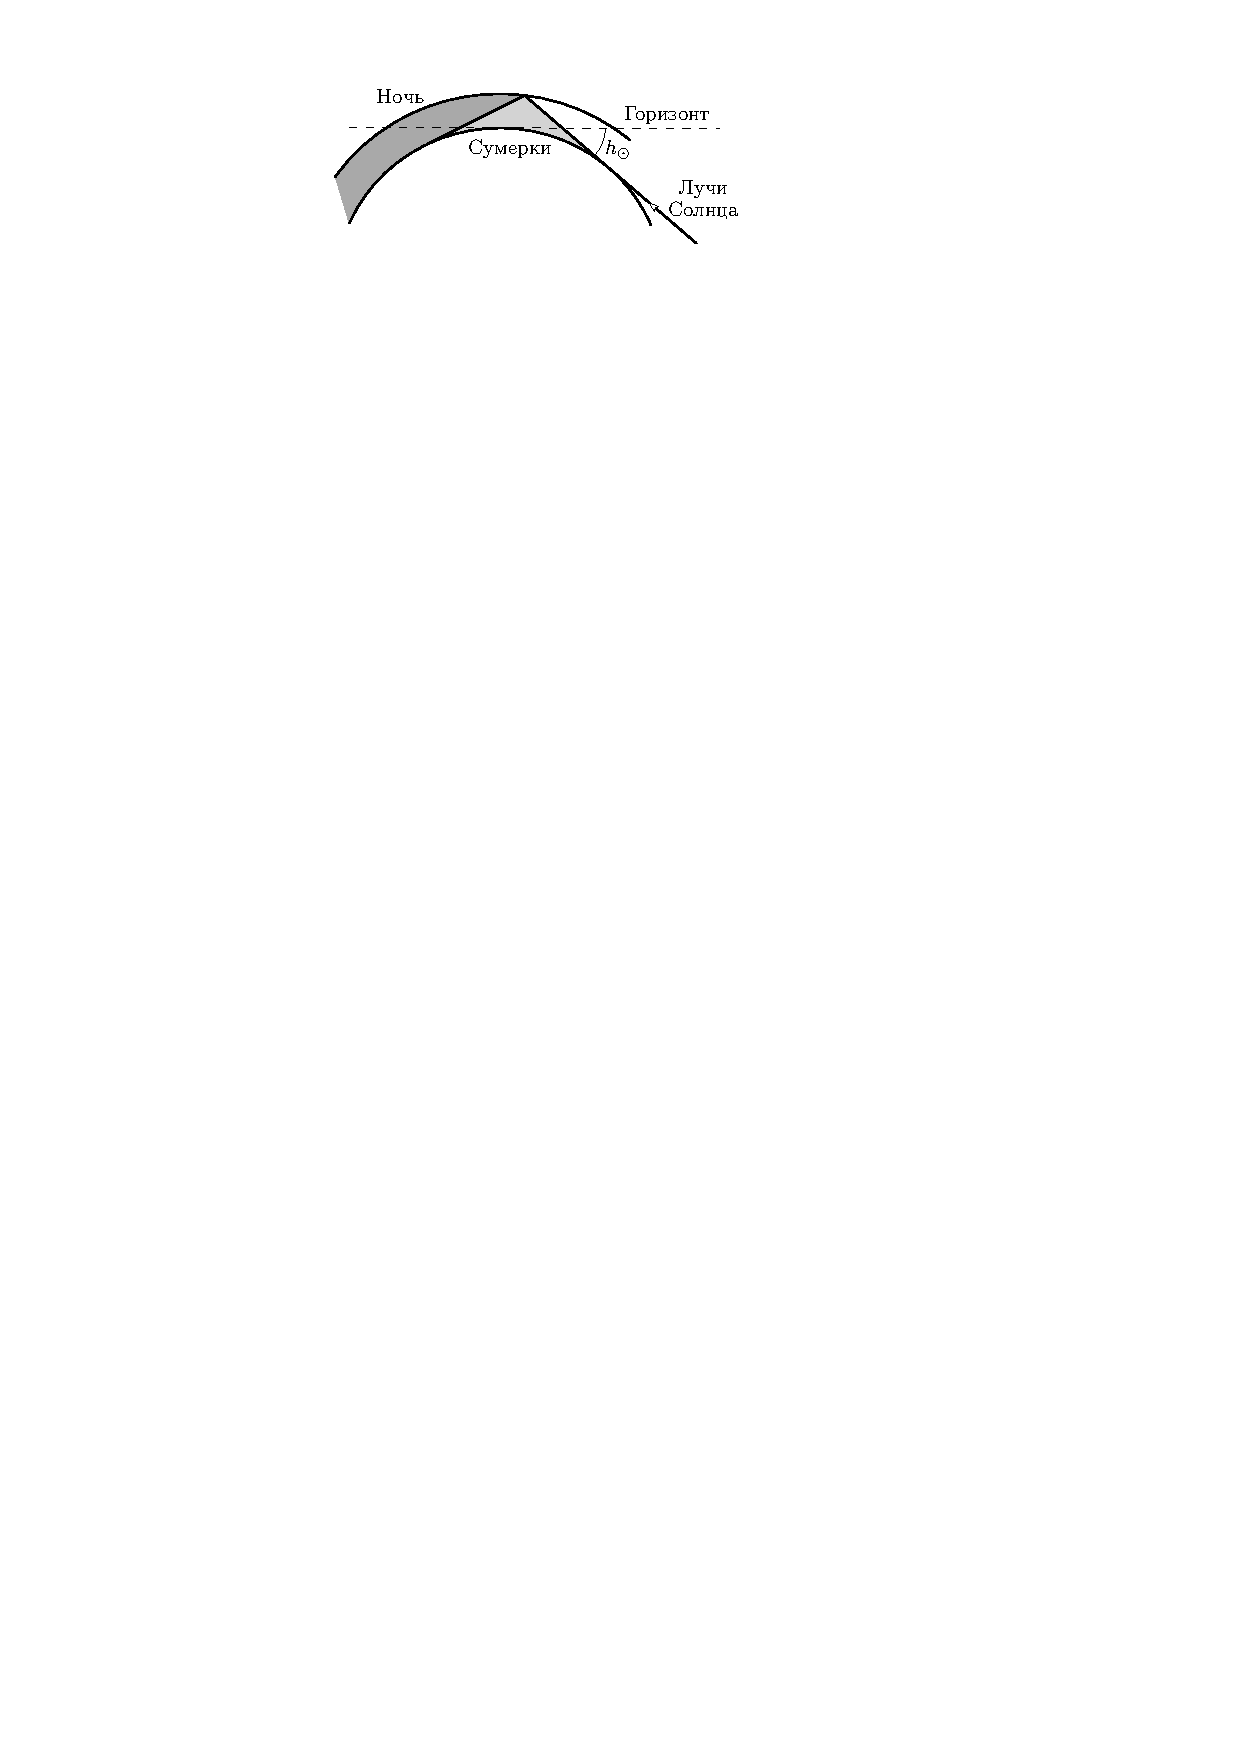
\includegraphics[width=\tw]{spher-astro-dusk.pdf}
	\captionof{figure}{Сумерки}
\end{minipage}
\newpage

	\section{Объекты космоса}
\subsection{Солнце}
\term{Солнце} --- центральное тело Солнечной системы, в нём сосредоточено 99,866\%  всей массы. Водород составляет~73\% общей массы Солнца, гелий~---~25\%. Остальные элементы: кислород, углерод, азот, магний, кремний, железо, сера, алюминий, натрий, кальций, никель и другие дают вклад всего~2\%.

По спектральной классификации Солнце~--- звезда типа G2V (жёлтый карлик на главной последовательности). Температура поверхности Солнца составляет $5 778$~К, поэтому Солнце светит почти в белом свете, но прямой свет Солнца у поверхности Земли приобретает жёлтый оттенок из-за рассеяния и поглощения коротковолновой части спектра в атмосфере.

Солнце вырабатывает энергию путём термоядерного синтеза. Каждую секунду в ядре около 4~млн.~тонн вещества превращается в лучистую энергию.\\

\term{Строение Солнца.}~~~В центре Солнца находится ядро с радиусом $150 $ -- $ 180$~тыс.~км, где идут термоядерные реакции. Плотность ядра около $1.5\times 10^5~\text{кг}/\text{м}^3$, а температура в его центре достигает $1.5\times 10^7$~К.

\begin{figure}[h!]
	\centering
	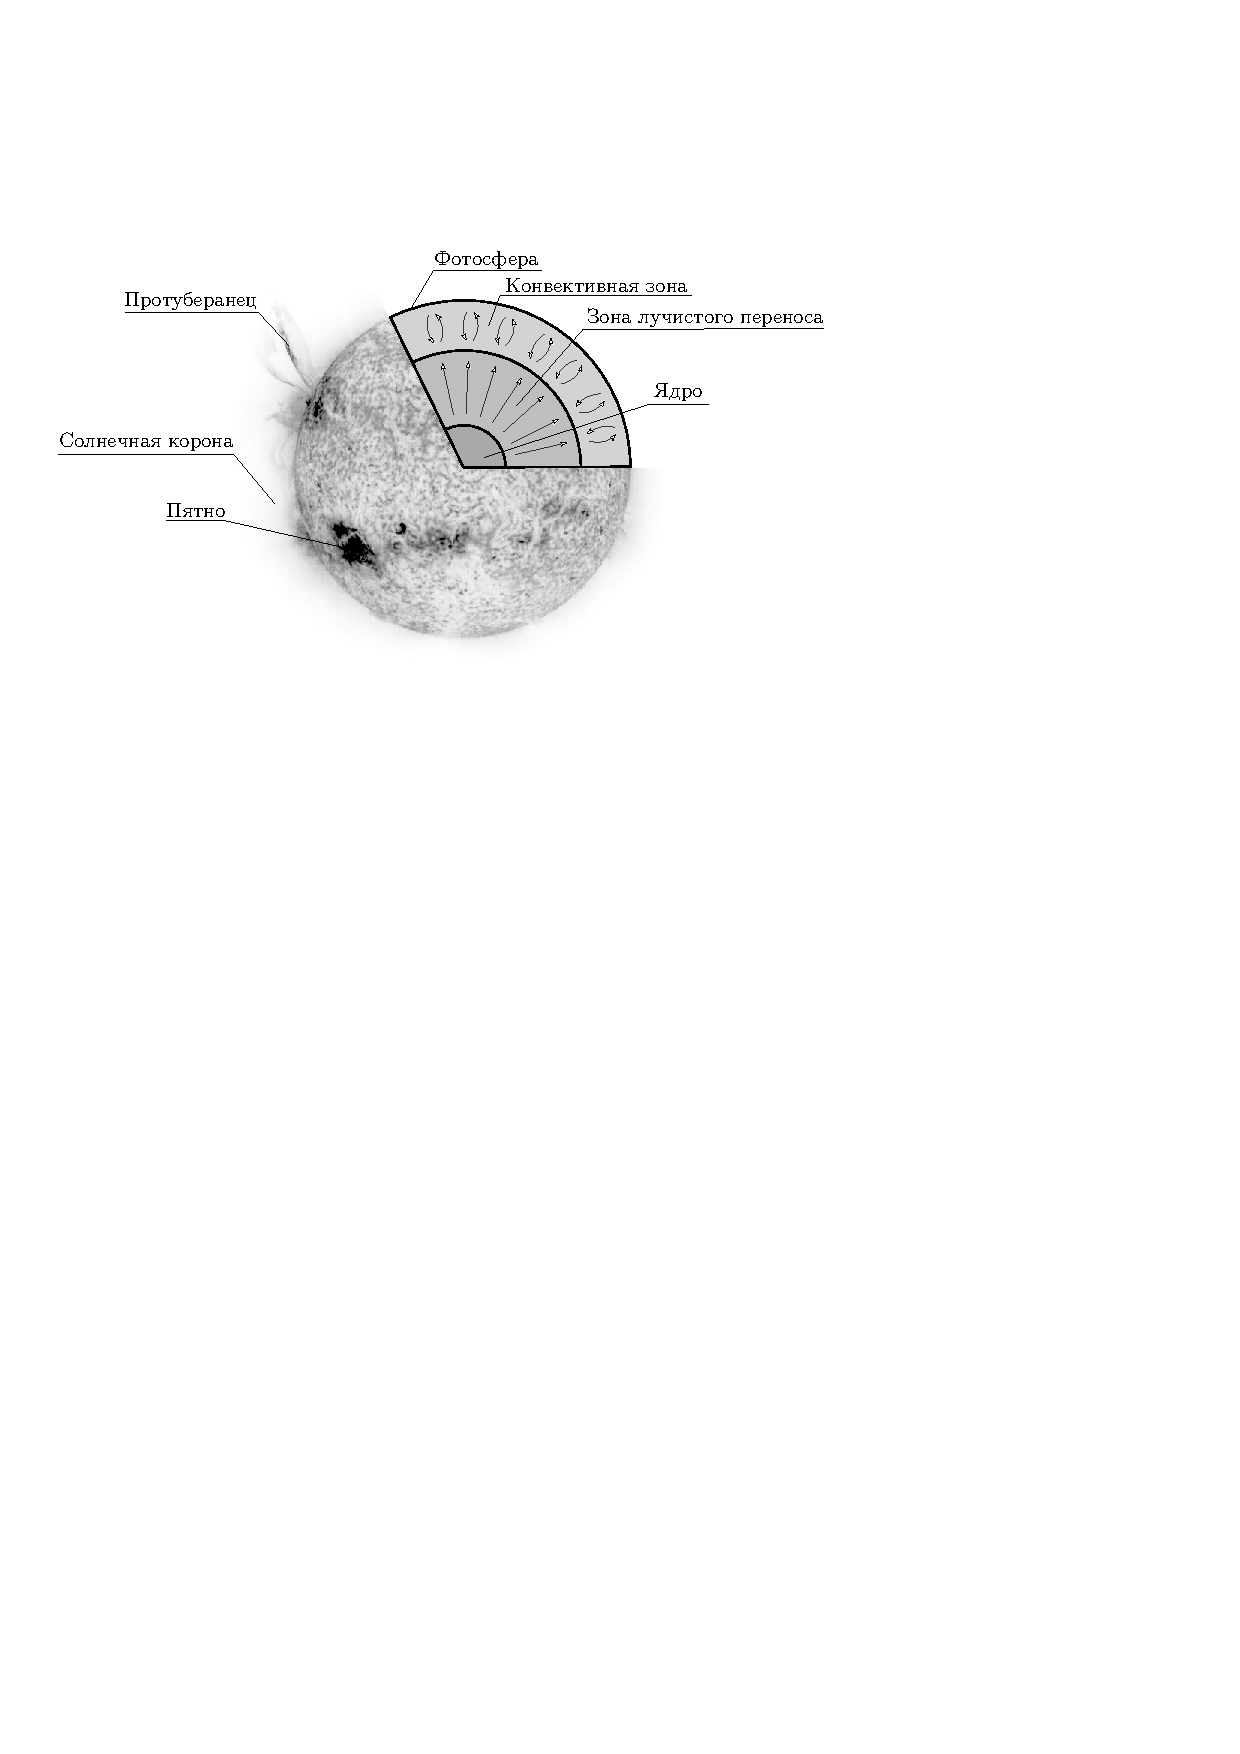
\includegraphics[width=0.8\textwidth]{sun.pdf}
	\caption{Строение Солнца. Фотография со спутника1 SOHO в фильтре $H_\alpha$ (негатив)}
\end{figure}
Над ядром, на расстояниях примерно от $0.25 R_\odot$ до $0.7R_\odot$ от его центра, находится \imp{зона лучистого переноса}. В этой зоне перенос энергии происходит главным образом с помощью излучения и поглощения фотонов. Температура в этой зоне лежит в интервале от $2\times10^6$~К сверху до $7\times10^6$~К снизу.

Над зоной лучистого  переноса (радиоактивная зона) находится \imp{конвективная зона}. Это слой толщиной примерно $2\times10^5$~км, в котором перенос энергии к поверхности совершается движением самого вещества. При приближении к поверхности конвективной зоны температура падает до $~5800$~К.

\textit{Фотосфера} --- видимая поверхность Солнца, по которой определяется размер Солнца. Эффективная температура фотосферы $T_\odot =  5778$~К.

\textit{Хромосфера} --- внешняя оболочка Солнца толщиной около 2000 км, окружающая фотосферу. Из хромосферы происходят горячие  выбросы вещества --- \textit{спикулы}. Температура хромосферы увеличивается с высотой до $2\times10^4$~К.

\textit{Солнечная корона} --- последний внешний слой Солнца, который состоит из протуберанцев и энергетических  извержений, образующих солнечный ветер. Средняя температура короны $2 \times 10^6$~К, а в некоторых частях достигает  и $20\times10^6$~К. Столь высокая температура обусловлена процессами, происходящими в магнитном поле звезды. Однако, несмотря на столь высокую температуру, корона видна лишь во время солнечных затмений, так как плотность её очень мала.

\term{Вращение Солнца} происходит не твердотельно~--- угловая скорость на разных широтах отличается, при удалении от экватора она уменьшается. Период вращения Солнца на разных широтах можно найти, наблюдая за солнечными пятнами и другими образованиями в фотосфере звезды. На экваторе период вращения составляет 25.05 суток, к полюсу он увеличивается до 34 суток. По наблюдениям за пятнами в течение длительного периода при помощи метода наименьших квадратов можно найти зависимость углового перемещения пятна за сутки от гелиографической широты:
\begin{equation}
	\Delta\lambda=14.37^{\circ}-2.7^{\circ}\sin^2\varphi,
\end{equation}
где $\Delta\lambda$~--- угловое перемещение пятна, $\varphi$~--- гелиографическая широта. Данная зависимость верна только для широт $\varphi < 40^\circ$.

\subsection{Спектральные классы звёзд}
\begin{table}[h!]
	\centering
	\footnotesize
	\renewcommand{\arraystretch}{1.4}
	\renewcommand{\tabcolsep}{0pt}
	\begin{tabularx}{\tw}{|C{0.1}|C{0.3}|C{0.23}|C{0.13}|C{0.13}|C{0.13}|}
		\hline
		{\bfseries Класс} & {$\mathbf{T}$, К} & {\bfseries Цвет} & {$\mathbf{M}$, $M_{\odot}$} & {$\mathbf{R}$, $R_{\odot}$} & {$\mathbf{L}$, $L_{\odot}$}\\
		\hline
		O & $3 \times 10^4$ --- $6 \times 10^4$ & Голубой & 60 & 15 & $1.4 \times 10^6$\\
		
		B & $1 \times 10^4$ --- $3 \times 10^4$ & Бело-голубой & 18 & 7 & $2 \times 10^4$\\
		
		A & $7.5 \times 10^3$ --- $1 \times 10^4$ & Белый & 3.1 & 2.1 & 80\\
		
		F & $6 \times 10^3$ --- $7.5 \times 10^3$ & Жёлто-белый & 1.7 & 1.3 & 6\\
		
		G & $5 \times 10^3$ --- $6 \times 10^3$ & Жёлтый & 1.1 & 1.1 & 1.2\\
		
		K & $3.5 \times 10^3$ --- $5 \times 10^3$ & Оранжевый & 0.8 & 0.9 & 0.4\\
		
		M & $2 \times 10^3$ --- $3.5 \times 10^3$ & Красный & 0.3 & 0.4 & 0.04\\
		\hline
	\end{tabularx}
	\caption{Современная спектральная классификация звёзд}
	\label{tab:spectr-types}
\end{table}
Звёзды в зависимости от своего цвета делятся на \imp{спектральные классы}, основные из них представлены в Таблице\,\ref{tab:spectr-types}. Масса, радиус и светимость приведены средних представителей спектрального класса, лежащих на главной последовательности (V).

Запись спектрального класса представляет собой латинскую букву, арабское число и римское число, например, спектральный класс Солнца~--- G2V. арабское число показывает к какой именно части спектрального класса относится звезда: к более синей (число меньше) или к красной (число больше). Так,~G10V~--- это тоже самое, что K0V. Спектральный класс (показатель цвета) и абсолютная звёздная величина задают положение звезды на \imp{Диаграмме Герцшпрунга-Рассела}.

\begin{figure}[h!]
	\centering
	\vspace{-1pc}
	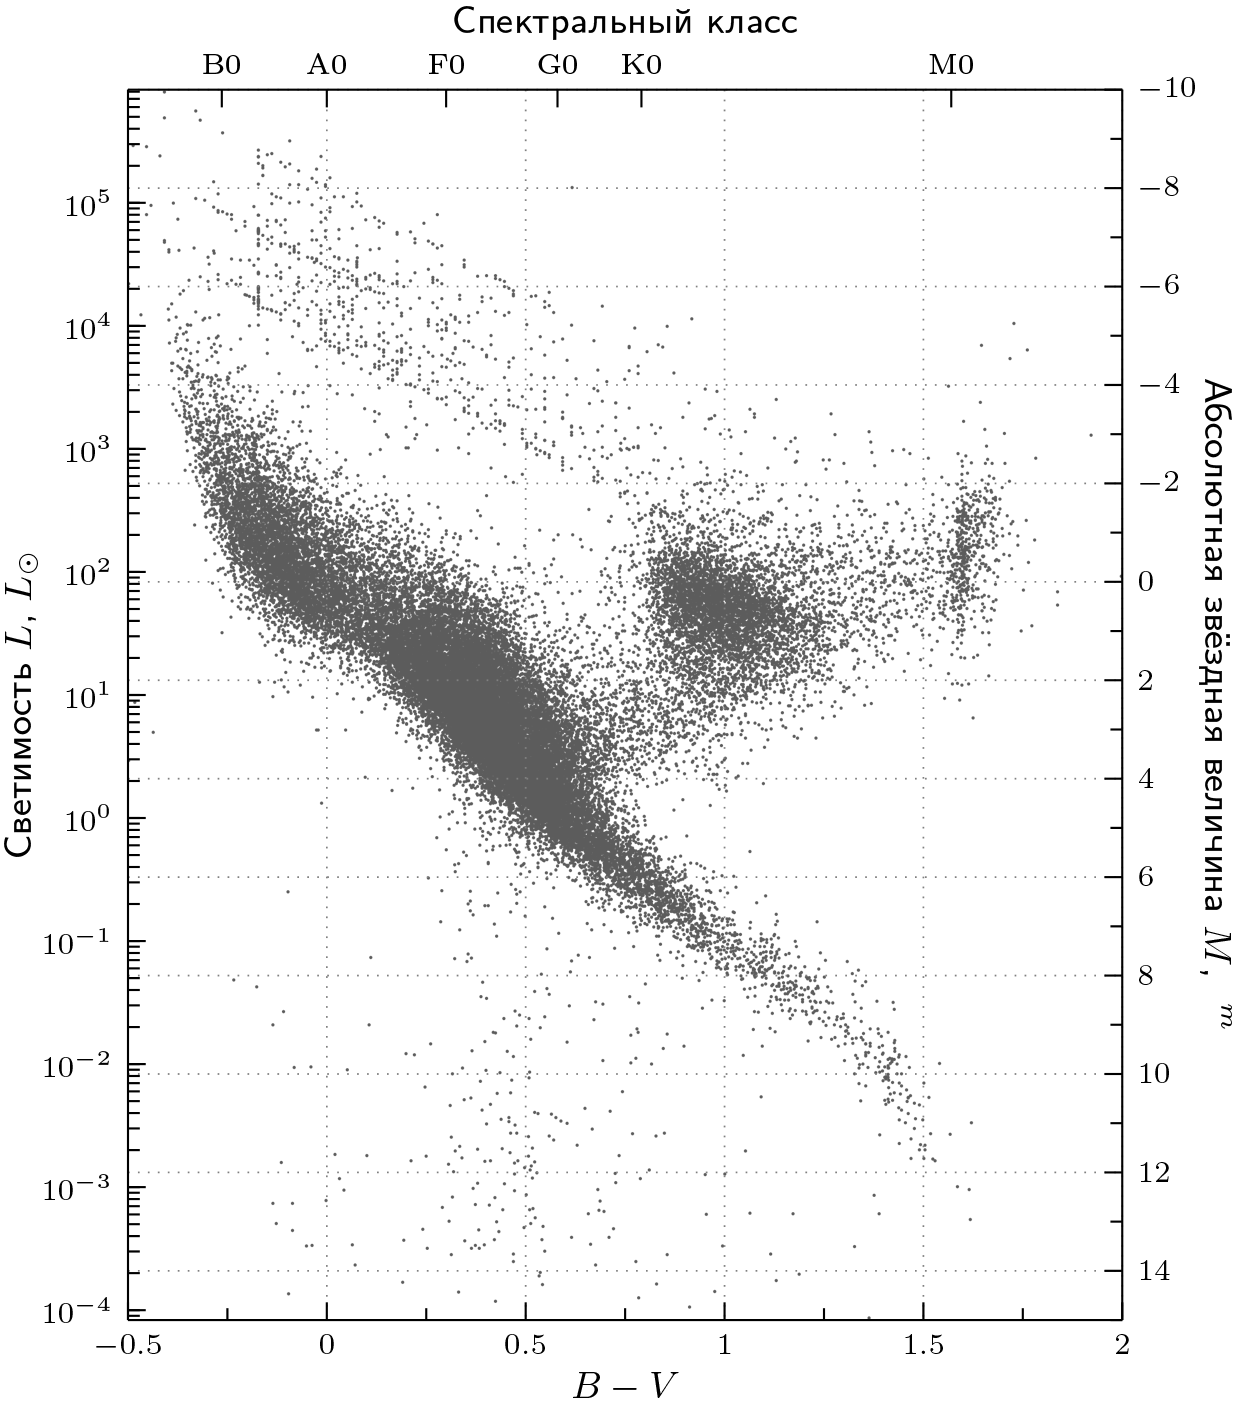
\includegraphics[width=10cm]{gr}
	\caption{Диаграмма Герцшпрунга--Рассела}
	\label{pic:d-cep}
\end{figure}
\term{Диаграмма Герцшпрунга-Рассела} показывает зависимость светимости или абсолютной звёздной величины от спектрального класса, показателя цвета $(B-V)$ или эффективной температуры фотосферы звезды.

Была предложена примерно в 1910 году независимо Эйнаром Герцшпрунгом и Генри Расселом. Диаграмма используется для классификации звёзд и соответствует современным представлениям о звёздной эволюции.

Около $90 \%$ звёзд находятся на главной последовательности. Их светимость обусловлена термоядерными реакциями превращения водорода в гелий. Выделяется также несколько ветвей проэволюционировавших звёзд-гигантов, в которых происходит горение гелия и более тяжёлых элементов. В левой нижней части диаграммы находятся полностью проэволюционировавшие белые карлики.

Мнемонические правила для запоминания спектральных классов: <<\textbf{O}h \textbf{B}e \textbf{A} \textbf{F}ine \textbf{G}irl, \textbf{K}iss \textbf{M}e \textbf{R}ight \textbf{N}ow \textbf{S}weetheart.>> и <<\textbf{В}ообразите: \textbf{О}дин \textbf{Б}ритый \textbf{А}нгличанин \textbf{Ф}иники \textbf{Ж}евал \textbf{К}ак \textbf{М}орковь --- \textbf{Р}азве \textbf{Н}е \textbf{С}мешно?>>

%	\begin{tikzpicture}
% 		\begin{axis}[
% 						height	=	12cm,
% 						width	=	10cm,
% 						ymax	=	15.,
% 						ymin	=	-10.,
% 						y dir	=	reverse,
% 						xmax	=	2.,
% 						xmin	=	-.5,
% 						axis x line* = bottom,
% 						axis y line* = right,
% 						xlabel=$B-V$,
% 						y label style = {at={(axis description cs: 1.2, 0.5)}, rotate=180},
% 						ylabel	=	{Абсолютная звёздная величина $M$, $~^m$}
% 					]
%%			\addplot+[only marks, mark = o, mark options={scale=0.2, black}] table[x=f, y=m]{data/light-curve-D-Cep.txt};
% 		\end{axis}
% 		\begin{semilogyaxis}[
% 						height	=	12cm,
% 						width	=	10cm,
% 						ymax	=	8.312e5,
% 						ymin	=	8.312e-5,
% 						xmax	=	2.,
% 						xmin	=	-.5,
% 						minor x tick num = 0,
% 						minor y tick num = 01,
% 						xtick = {-0.264, 0, 0.3, 0.58, 0.791, 1.57},
% 						xticklabels = {B0, A0, F0, G0, K0, M0},
% 						axis x line* = top,
% 						axis y line* = left,
% 						xlabel	=	{Спектральный класс},
% 						x label style = {at={(axis description cs: 0.5, 1.11)}, rotate=0},
% 						ylabel	=	{Светимость $L$, $L_\odot$},
% 						ymajorgrids	 =	false,
% 						xmajorgrids	 =	false
%    				]
%		\end{semilogyaxis}
% 	\end{tikzpicture}
Помимо основных спектральных классов звёзд существуют дополнительные: W~--- звёзды Вольфа-Райе, очень тяжёлые яркие звёзды с температурой порядка $70000$~К и интенсивными эмиссиоными линиями спектра; L~--- звёзды или коричневые карлики с температурой 1500\,--\,2000~К и соединениями металлов в атмосфере; T~--- метановые коричневые карлики с температурой $700 - 1500$~К; Y~---  очень холодные (метано-аммиачные) коричневые карлики с температурой ниже $700$~К; C~--- углеродные звёзды, гиганты с повышенным содержанием углерода. Ранее относились к классам R и N.

\subsection{Переменные звёзды}
\term{Переменные звёзды}~--- звёзды, у которых наблюдаются колебания блеска.   Для отнесения звезды к разряду переменных достаточно, чтобы блеск звезды хотя бы однажды претерпел изменение.

Переменные звёзды делятся на две большие группы: \imp{затменные} и \imp{физические}, причём физические подразделяются на \imp{пульсирующие} и \imp{эруптивные}.

\begin{wrapfigure}[11]{l}{0.5\tw}
	\centering
	\vspace{-1.2pc}
	\begin{tikzpicture}
		\begin{axis}[
			height	=	4.5cm,
			width	=	.5\tw,
			xlabel	=	{Фаза},
			ylabel	=	{Блеск $m$, $~^m$},
			ymax	=	8.,
			ymin	=	6.5,
			y dir	=	reverse,
			xmax	=	1,
			xmin	=	0
			]
			\addplot+[only marks, mark = o, mark options={scale=0.2, black}] table[x=f, y=m]{data/light-curve-D-Cep.txt};
		\end{axis}
	\end{tikzpicture}
	\caption{Кривая блеска переменной типа $\delta$\,Cep}
	\label{pic:d-cep}
\end{wrapfigure}
К \term{пульсирующим} переменным  относят те звёзды, переменность которых вызвана процессами, происходящими в их недрах. Эти процессы приводят к периодическому изменению температуры поверхности и радиуса фотосферы, а вместе с ними и блеска звезды. Период переменности варьируется в пределе от долей суток до~нескольких~лет в зависимости от типа переменной.

Классический пример пульсирующих переменных звёзд~--- \imp{цефеиды}, названные в честь первой открытой переменной данного типа~--- $\delta$\,Cep. Абсолютную звёздную величину $M$ и период $T$ (в сутках) цефеид связывает соотношение
\begin{equation}
	M = -1.43^m - 2.81\lg T.
\end{equation}
К \term{эруптивным} переменным звёздам относятся звёзды, меняющие свой блеск нерегулярно или единожды за время наблюдений. Все изменения блеска эруптивных звёзд связывают с бурными процессами и вспышками в их хромосферах и коронах. К таким, например, относятся \imp{новые} и \imp{сверхновые}.

\term{Затменно-переменные} звёзды --- системы из двух звёзд, суммарный блеск которых периодически изменяется с течением времени. Причиной изменения блеска могут быть затмения звёзд друг другом, или изменение их формы взаимной гравитацией в тесных системах. На Рис.\,\ref{pic:w-uma}\,--\,\ref{pic:b-lyr}  представлены кривые блеска затменно-переменных звёзд трёх основных типов.

\begin{figure}[!h]
	\centering
	\begin{minipage}[c]{0.49\tw}
		\begin{tikzpicture}
			\begin{axis}[
				height	=	4.5cm,
				width	=	\tw,
				xlabel	=	{Фаза},
				ylabel	=	{Блеск $m$, $~^m$},
				ymax	=	1.1,
				ymin	=	-.1,
				y dir	=	reverse,
				xmax	=	1,
				xmin	=	0
				]
				
				\addplot[smooth] table[x=t, y=m]{data/light-curve-W-UMa.txt};
			\end{axis}
		\end{tikzpicture}
	\end{minipage}
	\hfill
	\begin{minipage}[c]{0.49\tw}
		\centering
		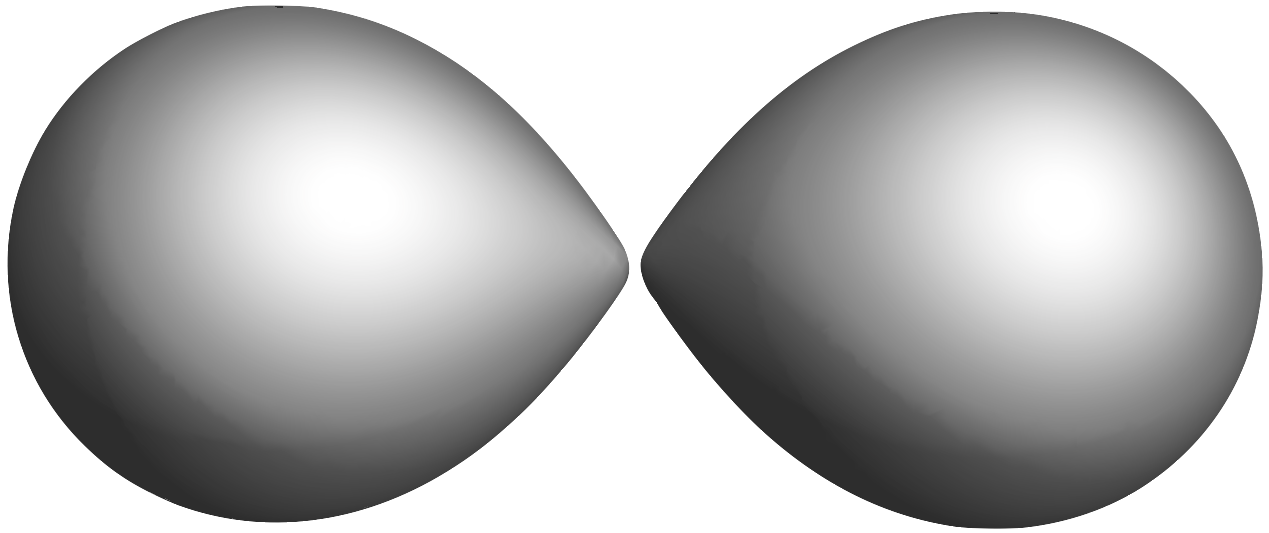
\includegraphics[width = .9\tw]{w-uma}
	\end{minipage}
	\caption{Кривая блеска переменной типа W\,UMa}
	\label{pic:w-uma}
\end{figure}

\begin{figure}[!h]
	\centering
	\begin{minipage}[c]{0.49\tw}
		\begin{tikzpicture}
			\begin{axis}[
				height	=	4.5cm,
				width	=	\tw,
				xlabel	=	{Фаза},
				ylabel	=	{Блеск $m$, $~^m$},
				ymax	=	.7,
				ymin	=	-.1,
				y dir	=	reverse,
				xmax	=	1.,
				xmin	=	.0
				]
				\addplot[smooth] table[x=t, y=m]{data/light-curve-B-Per.txt};
			\end{axis}
		\end{tikzpicture}
	\end{minipage}
	\hfill
	\begin{minipage}[c]{0.49\tw}
		\centering
		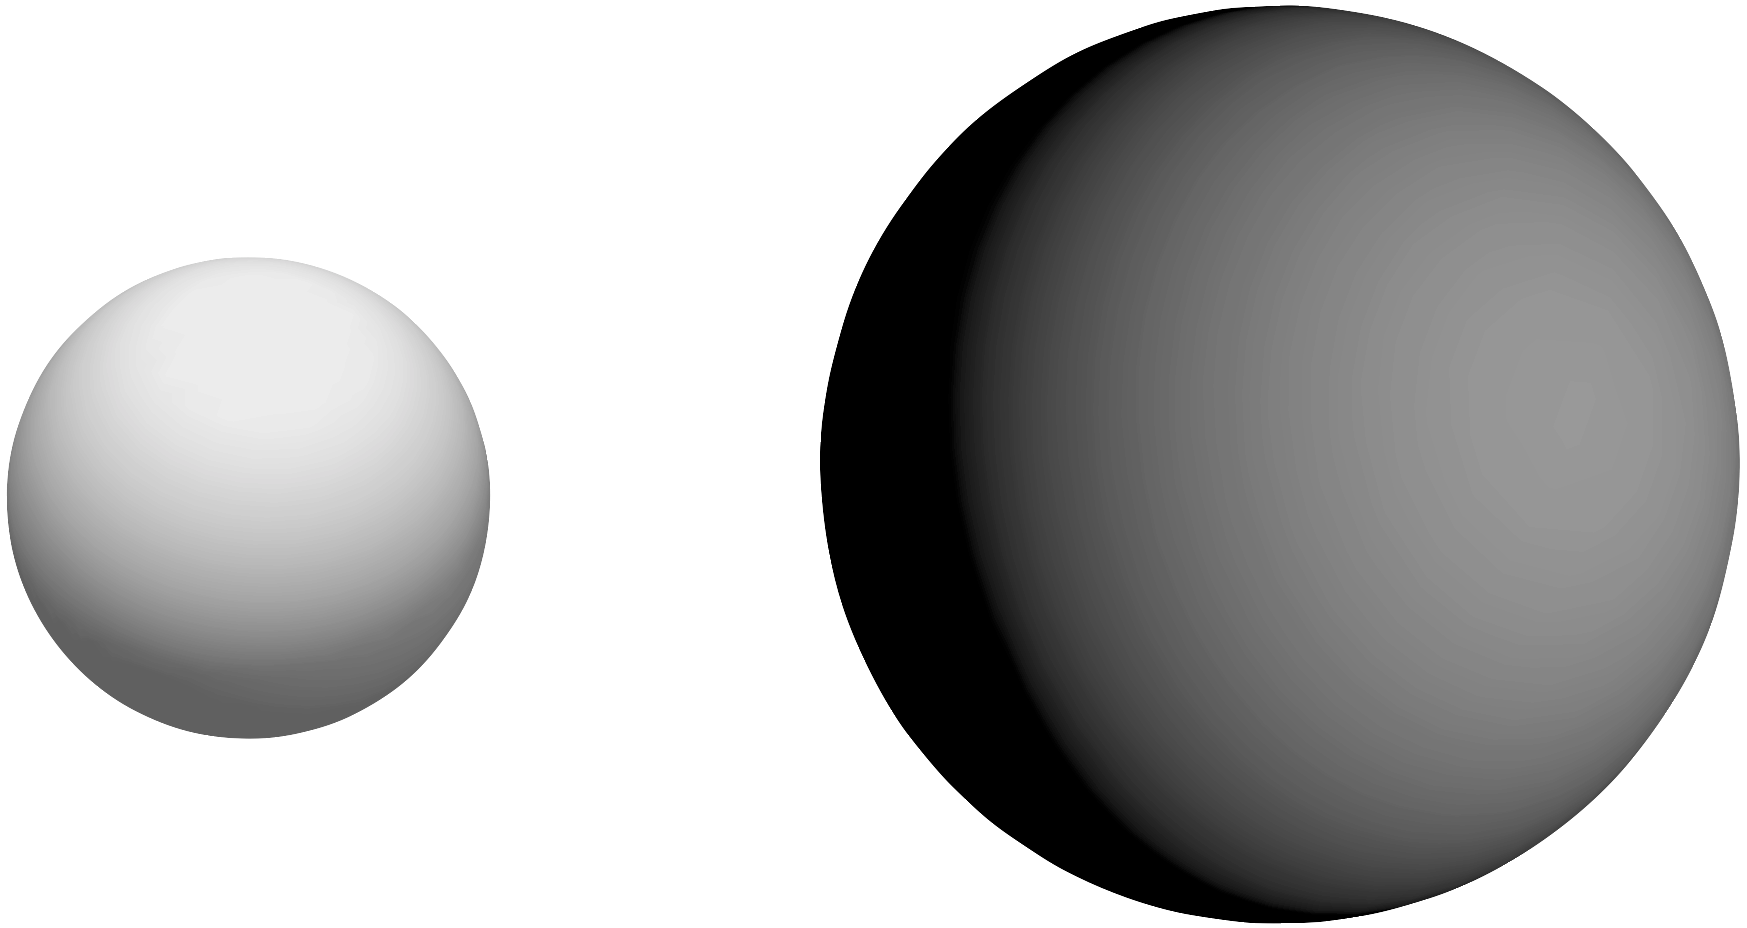
\includegraphics[width=.9\tw]{b-per}
	\end{minipage}
	\caption{Кривая блеска переменной типа $\beta$\,Per}
\end{figure}

\subsection{Вырожденные звёзды}
\term{Вырожденные звезды}~--- звезды, в которых силам гравитации противостоят силы давление вырожденного газа. К таким относятся \imp{белые карлики} и \imp{нейтронные звезды}. 

\begin{figure}[!h]
	\centering
	\begin{minipage}[c]{0.49\tw}
 		\begin{tikzpicture}
 			\begin{axis}[
 							height	=	4.5cm,
 							width	=	\tw,
 							xlabel	=	{Фаза}, 
 							ylabel	=	{Блеск $m$, $~^m$}, 
 							ymax	=	.7,
 							ymin	=	-.1,
 							y dir	=	reverse,
 							xmax	=	1,
 							xmin	=	.0
 						]
				\addplot[smooth] table[x=t, y=m]{data/light-curve-B-Lyr.txt};
 			\end{axis}
 		\end{tikzpicture}
 	\end{minipage}
 	\hfill
 	\begin{minipage}[c]{0.49\tw}
 		\centering
 		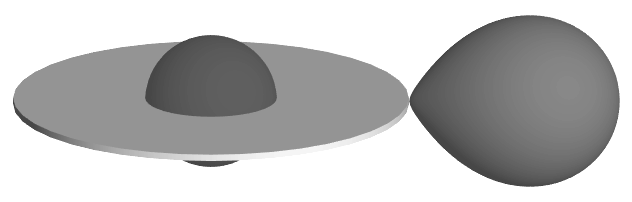
\includegraphics[width = .9\tw]{b-lyr}	
 	\end{minipage}
 	\caption{Кривая блеска переменной типа $\beta$\,Lyr}
 	\label{pic:b-lyr}
 	\vspace{-.8pc}
\end{figure}
\term{Белые карлики}~--- проэволюционировавшие звёзды лишённые собственных источников термоядерной энергии. Масса белого карлика находится в диапазоне от $0.6M_{\odot}$ до $1.44 M_{\odot}$. Верхняя границы массы белого карлика называется пределом Чандрасекара, звезда с массой больше данного предела не может существовать как белый карлик. Радиус белых карликов примерно в $10^2$ раз меньше солнечного, т.е. можно считать, что $R_\text{БК} \simeq R_\oplus$. Плотность белых карликов лежит в диапазоне $10^7$\,--\,$10^{10}$~$\text{кг}/\text{м}^3$.

\term{Нейтронная звезда}~--- сверхплотная звезда, образующаяся в результате взрыва Сверхновой. Вещество нейтронной звезды состоит в основном из нейтронов. Масса нейтронной звезды лежит в пределах от $0.1M_{\odot}$ до $2$\,--\,$2.8M_{\odot}$ (предел Оппенгеймера-Волкова). Размер данной звезды составляет лишь $10$\,--\,$20$~км, а плотность составляет $10^{16}$\,--\,$10^{18}$ $\text{кг}/\text{м}^3$.  Дальнейшему гравитационному сжатию нейтронной звезды препятствует давление ядерной материи, возникающее за счёт взаимодействия нейтронов. Так как нейтронные звёзды образуются в результате  коллапса массивных звёзд, то из-за сохранения момента импульса скорость их вращения очень велика~--- максимальная скорость может достигать $10^5$~км/с.
\subsection{Чёрные дыры}
\term{Чёрная дыра}~(ЧД)~--- область пространства-времени с массой $M$, гравитационное притяжение которой настолько велико, что покинуть её не могут даже объекты, движущиеся со скоростью света $c$. Граница этой области называется \imp{горизонтом событий}, а её характерный размер~$R_G$~--- \imp{гравитационным радиусом}, для величины которого справедливо равенство
\begin{equation}
R_G = \frac{2 G M}{c^2}.
\end{equation}

Минимальная масса ЧД составляет около $2.5M_{\odot}$. А плотность ЧД определяется отношением ее массы~$M$ к~объему~$V$, следовательно
\begin{equation}
\rho = \frac{M}{V} = \frac{3c^6}{32\pi M^2G^3}.
\end{equation}

\term{Эффект излучения} (испарения) \term{Хокинга}~--- эффект, при котором гравитационное поле черной дыры поляризует вакуум, в результате чего возможно образование не только виртуальных, но и реальных пар частица~--античастица. Одна из частиц, оказавшаяся чуть ниже горизонта событий, падает внутрь чёрной дыры, а другая, оказавшаяся чуть выше горизонта, улетает, унося энергию (то есть часть массы) чёрной дыры. Для мощности излучения ЧД справедлива формула
\begin{equation}
L = \frac{h c^6}{30720 \pi^2 G^2 M^2},
\end{equation}
где $h$ --- постоянная Планка. Спектр хокинговского излучения для безмассовых полей оказался строго совпадающим с излучением абсолютно чёрного тела, что позволило приписать ЧД температуру, равную
\begin{equation}
T = \frac{h c^3}{16 \pi^2 k G M},
\end{equation}
где $k$ --- постоянная Больцмана.
\subsection{Галактики}
\term{Морфологическая классификация галактик}~--- система разделения галактик на группы по визуальным признакам, используемая в астрономии. Наиболее известной является классификация, разработанная Хабблом и дополненная другими учеными. 
	\begin{figure}[h!]
		\centering
		\vspace{-.9pc}
		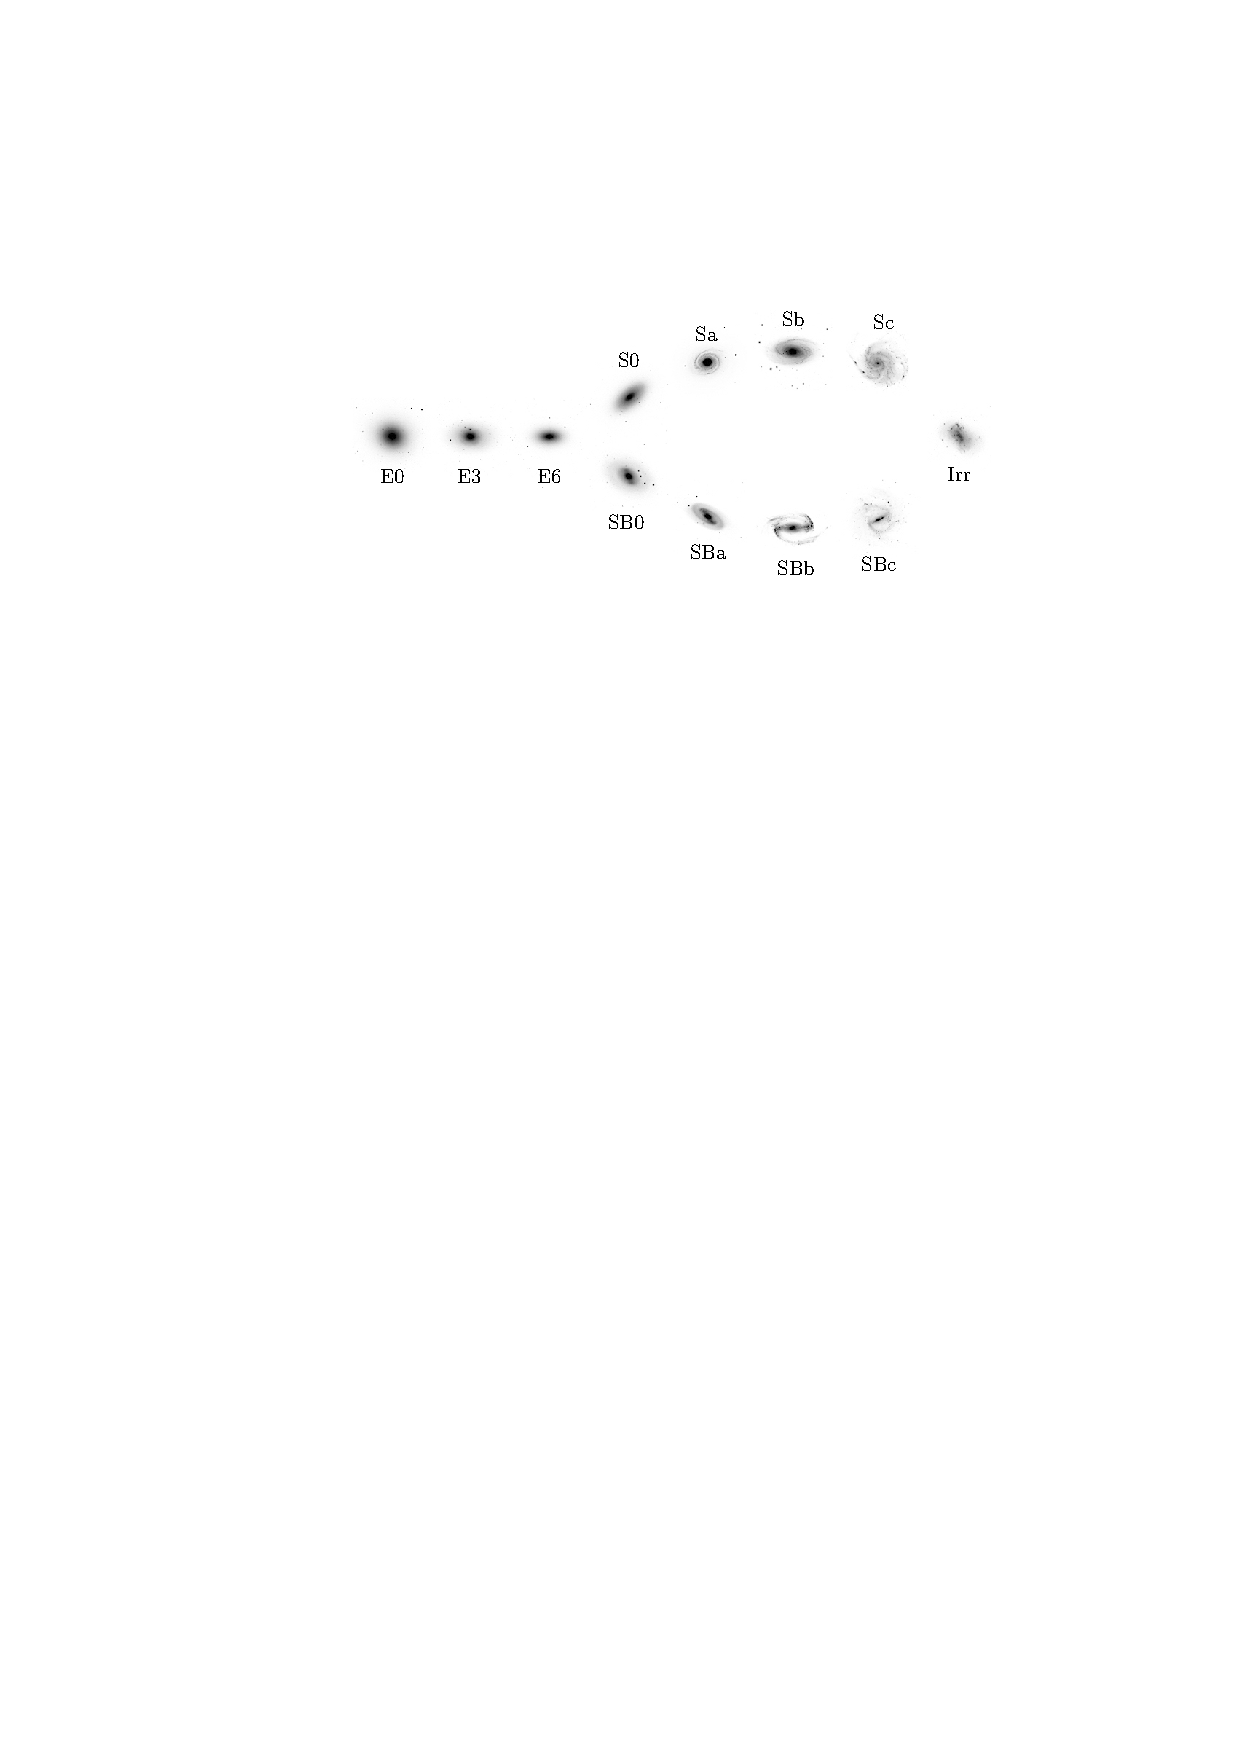
\includegraphics[width=0.65\tw]{hubble-fork.pdf}
		\caption{<<Вилка Хаббла>>}
	\end{figure}
	
Согласно данной классфикации галактики делятся на 4 типа:
\begin{enumerate}[itemsep=3pt, label={\arabic*.}, leftmargin=1pc]
	\item{\term{Эллиптические галактики} имеют гладкую эллиптическую форму без отличительных деталей с равномерным уменьшением яркости от центра к периферии. Обозначаются буквой E с индексом. Индекс можно рассчитать по формуле
		\begin{equation}
		i = 10 \cdot \left(1 - \frac{b}{a}\right),
		\end{equation}\nopagebreak
		где $a$ и $b$~--- большая и малая полуоси видимого эллипса. 
		
		К линзовидным галактикам с абсолютной звёздной величиной около $-21^m$ применимо соотношение Фабер-Джексона:
		\begin{equation}
			L \propto \sigma^4,
		\end{equation}
		где $\sigma$~--- дисперсия скоростей вещества в галактике.}
	\item{\term{Спиральные галактики} состоят из уплощенного диска из звезд и газа, в центре которого находится сферическое уплотнение, называемое балджем, а также обширного сферического гало. Спиральные галактики обозначаются SB при наличии бара (перемычки между рукавами) или S при отсутствии бара. В зависимости от размеров ядра и балджа галактики делят на 3 группы: a, b и c. Для галактик Sa характерен большой балдж, для галактик Sc~--- маленький. Галактики Sb представляют собой нечто среднее между галактиками Sa и Sc.
	
	Светимость спиральных галактик $L$ связана с их максимальной скоростью вращения $v_\text{макс}$ \term{соотношением Талли-Фишера}:
	\begin{equation}
		L \propto v_\text{макс}^4.
	\end{equation}
	Абсолютная звёздная величина Млечного пути $M_\text{MW} \simeq -21^m$.}
	\item{\term{Неправильные или иррегулярные галактики}~--- галактика, лишенная как вращательной симметрии, так и значительного ядра. Обозначение: Irr.}
	\item{\term{Линзовидные галактики}~--- галактики, являющиеся переходными между спиральными и эллиптическими. Обозначения: S0, SB0.}
\end{enumerate}


\subsection{Другие объекты}
\begin{minipage}{0.63\tw}
\term{Шаровое звёздное скопление}~--- скопление звёзд, состоящее из нескольких сотен тысяч светил, тесно связанных гравитацией. Млечный путь насчитывает около 160 шаровых звёздных скоплений. Диаметры шаровых скоплений составляют 20\,--\,60~пк, массы~--- $10^4$\,--\,$10^6$~солнечных.\par

\term{Планетарная туманность}~--- система из звезды, называемой ядром туманности, и симметрично окружающей ее светящейся газовой оболочки. Планетарные туманности образуются при сбросе внешних слоёв (оболочек) красных гигантов и сверхгигантов с массой от $0.8M_\odot$ до $8M_\odot$ на завершающей стадии их эволюции. Характерный размер~--- 1\,--\,2~св.\,лет.
\end{minipage}
\hfill
\begin{minipage}{0.32\tw}
	\centering
	\vspace{-1.2pc}
	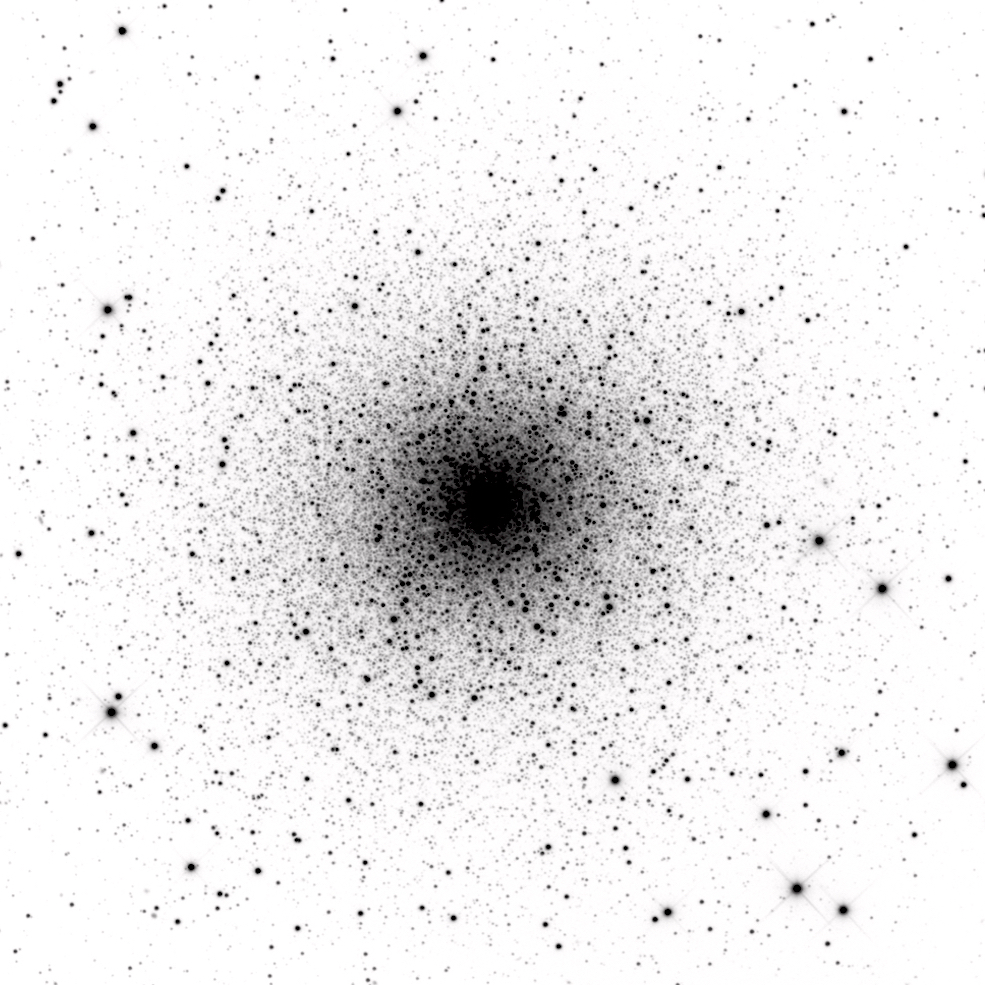
\includegraphics[width = .55\tw]{m13}
	\captionof{figure}{Шаровое скопление M13 (негатив)}
	\vspace{1pc}
	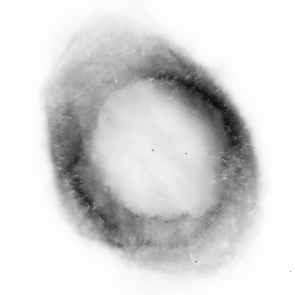
\includegraphics[width = .55\tw]{m57}
	\captionof{figure}{Пла\-не\-тар\-ная туманность M57 (негатив)}
\end{minipage}
	\newpage
\section{Математика}
\subsection{Системы координат}

\begin{wrapfigure}{r}{0.27\tw}
	\centering
	\vspace{-1pc}
	\begin{tikzpicture}[scale=1]
		\footnotesize
		\coordinate (O) at (0, 0);
		\coordinate (E1) at (2, 0);
		\coordinate (E2) at (1, 0.5);
		\coordinate (E3) at (0.5, 1.5);
		\coordinate (M) at (2, 2);
		
		\draw[semithick, -latex] (O) -- (E1);
		\draw[semithick, -latex] (O) -- (E2);
		\draw[semithick, -latex] (O) -- (E3);
		\draw[thick, -latex] (O) -- (M);
		
		\point (O);
		\point (M);
		
		\draw (1, 0) node[anchor=north]{$\vec{e}_1$};
		\draw (0.66, 0.33) node[anchor=north]{$\vec{e}_2$};
		\draw (0.25, 0.75) node[anchor=east]{$\vec{e}_3$};
		\draw (1, 1.05) node[anchor=south]{$\vec{r}$};
		\draw (M) node[anchor=north west]{$M$};
		\draw (O) node[anchor=north east]{$O$};
	\end{tikzpicture}
	\caption{}
	\vspace{-1pc}
	\label{pic:math-coord-sys-decart}
\end{wrapfigure}
Зафиксируем точку $O$ в пространстве и рассмотрим произвольную точку $M$. Вектор $\vec{r} = \overrightarrow{OM}$ называется радиус-вектором точки $M$. Пусть в рассматриваемом пространстве также выбран базис $\{\vec{e}_1, \ldots, \vec{e}_n \}$, тогда совокупность точка $O$ и базиса называется \term{декартовой системой координат}. Причем точка $O$~--- начало координат, а базисные векторы $\vec{e}_1, \ldots, \vec{e}_n$ задают координатные оси.

\begin{wrapfigure}{r}{0.27\tw}
	\centering
	\vspace{-1pc}
	\begin{tikzpicture}[scale=1]
		\footnotesize
		\coordinate (O) at (0, 0);
		\coordinate (E1) at (1.5, 0);
		\coordinate (E2) at (-1, -0.5);
		\coordinate (E3) at (0, 1.5);
%		\coordinate (M) at (2, 2);
		
		\draw[semithick, -latex] (O) -- (E1);
		\draw[semithick, -latex] (O) -- (E2);
		\draw[semithick, -latex] (O) -- (E3);
%		\draw[thick, -latex] (O) -- (M);
		
		\point (O);
%		\point (M);
		
		\draw (-0.5, -0.25) node[anchor=south]{$\vec{e}_1$};
		\draw (0.75, 0) node[anchor=south]{$\vec{e}_2$};
		\draw (0, 0.75) node[anchor=east]{$\vec{e}_3$};
%		\draw (1, 1.05) node[anchor=south]{$\vec{r}$};
%		\draw (M) node[anchor=south]{$M$};
		\draw (0, -0.1) node[anchor=north]{$O$};
		
		\draw (0, 0.25) -- (0.25, 0.25) -- (0.25, 0);
		\draw (0.25, 0) -- (0.027, -0.112) -- (-0.223, -0.112);
		\draw (0, 0.25) -- (-0.223, 0.138) -- (-0.223, -0.112);
	\end{tikzpicture}
	\caption{}
	\vspace{-1pc}
	\label{pic:math-coord-sys-ord-basis}
\end{wrapfigure}
Однако пользоваться представлением векторов в произвольном базисе довольно сложно, поэтому рассмотрим специальный тип~--- \term{орто\-нор\-ми\-рованный базис}~--- это такой базис, базисные векторы которого попарно ортогональны, и длина каждого равна единице.

\term{Прямоугольной декартовой системой координат} (ПДСК) называют декартову систему координат с ортонормированным базисом. В практических задачах использовать ПДСК не всегда удобно, поэтому также рассмотрим другие системы координат. 

\begin{wrapfigure}{r}{0.27\tw}
	\centering
	\vspace{-1pc}
	\begin{tikzpicture}[scale=1]
		\clip(-1.05, -1.55) rectangle (2.1, 1.55);
	
		\footnotesize
		\coordinate (O) at (0, 0);
		\coordinate (E1) at (2, 0);
%		\coordinate (E2) at (1, 0.5);
%		\coordinate (E3) at (0.5, 1.5);
		\coordinate (M) at (1, 1);
		
		\draw[semithick, -latex] (O) -- (E1);
%		\draw[semithick, -latex] (O) -- (E2);
%		\draw[semithick, -latex] (O) -- (E3);
		\draw[thick, -latex] (O) -- (M);
		\draw[-latex] (0.65, 0) arc(0:45:0.65);
		
		\foreach \r in {0.5, 1, 1.5} {
			\draw (O) circle(\r);
		};
		
		\point (O);
		\point (M);
		
		\draw (1.2, 0) node[anchor=north]{$\vec{r}_0$};
%		\draw (0.66, 0.33) node[anchor=north]{$\vec{e}_2$};
%		\draw (0.25, 0.75) node[anchor=east]{$\vec{e}_3$};
		\draw (0.5, 0.5) node[anchor=south]{$\vec{r}$};
		\draw (0.55, 0.3) node[anchor=west]{$\varphi$};
		\draw (1, 0.9) node[anchor=south east]{$M$};
		\draw (O) node[anchor=north east]{$O$};
	\end{tikzpicture}
	\caption{}
	\label{pic:math-coord-sys-polar}
\end{wrapfigure}
На плоскости, то есть в пространстве $\R^2$, имеющем размерность два, часто применяется \term{полярная система координат}. В ней координатами вектора является его длина $r$~--- расстояние до точки от начала отсчёта, и угол $\varphi$ радиус-вектора с начальной ось.

Пусть $(x,y)$~--- координаты некоторого вектора в ПДСК на $\R^2$, тогда не сложно получить, что его координаты в полярной системе координат (начальная ось совпадает с осью $Ox$)  удовлетворяют следующим соотношениям:
\begin{equation}
	\begin{cases}
		r = \sqrt{x^2 + y^2},\\
		\sin \varphi = y/r,\\
		\cos \varphi = x/r.
	\end{cases}
	\quad \Leftrightarrow \quad
	\begin{cases}
		x = r \cos \varphi,\\
		y = r \sin \varphi.
	\end{cases}
\end{equation}

\begin{wrapfigure}{r}{0.35\tw}
	\centering
%	\vspace{-1pc}
	\begin{tikzpicture}[scale=1]
		\clip(-1.3, -1.1) rectangle (2.5, 2.5);
	
		\footnotesize
		\coordinate (O) at (0, 0);
		\coordinate (E1) at (2.3, 0);
		\coordinate (E2) at (0, 2.3);
		\coordinate (E3) at (-1, -1);
		\coordinate (M) at (0.8, 1.3);
		\coordinate (M') at (0.8, -0.48);
		\coordinate (M'') at (1, -0.6);
		
		\draw[semithick, -latex] (O) -- (E1);
		\draw[semithick, -latex] (O) -- (E2);
		\draw[semithick, -latex] (O) -- (E3);
		\draw[thick, -latex] (O) -- (M);
		
		\draw [dashes] (0, 1.78) -- (M) -- (M');
		\draw [dashes] (M'') -- (O);
		\draw [dashes] (1.28, 0) -- (M') -- (-0.48, -0.48);
		
		\draw (O) ellipse(2 and 0.7);
		\draw (0, 1.78) ellipse(2 and 0.7);
		
		\draw [-latex](-0.2, -0.2) arc(-99.4:-75.76:1.22);

        \foreach \p in {O, M, M', M''} {
            \point (\p);
        };
		
		\draw (0.5, 0.65) node[anchor=south east]{$\vec{r}$};		
		\draw (0.05, -0.15) node[anchor=north]{$\varphi$};
		\draw (0.42, -0.2) node[anchor=west]{$r$};
		\draw (0.8, 0.4) node[anchor=west]{$h$};
		\draw (M) node[anchor=south west]{$M$};
		\draw (O) node[anchor=south east]{$O$};
		
		\draw (E1) node[anchor=north]{$y$};
		\draw (E2) node[anchor=east]{$z$};
		\draw (E3) node[anchor=east]{$x$};
	\end{tikzpicture}
	\caption{}
	\label{pic:math-coord-sys-cyl}
	\vspace{-2pc}
\end{wrapfigure}
Теперь пусть $(x, y, z)$~--- координаты некоторого вектора в ПДСК на~$\R^3$. Обозначим за $h$~--- длину проекции этого вектора на ось $z$, $r$~--- длину его проекции на плоскость $Oxy$, $\varphi$~--- угол между проекцией на плоскость $Oxy$ и осью $Ox$. Тогда тройка $(r, \varphi, h)$~--- координаты рассматриваемого векторы в \term{цилиндрической системе координат}, и верно представление
\begin{equation}
	\begin{cases}
		r = \sqrt{x^2 + y^2},\\
		\sin \varphi = y/r,\\
		\cos \varphi = x/r,\\
		h = z.
	\end{cases}
	\quad \Leftrightarrow \quad
	\begin{cases}
		x = r \cos \varphi,\\
		y = r \sin \varphi,\\
		z = h.
	\end{cases}
\end{equation}

\begin{wrapfigure}{r}{0.35\tw}
	\centering
	\vspace{-2.5pc}
	\begin{tikzpicture}[scale=1]
		\clip(-1.3, -1.1) rectangle (2.5, 2.5);
%	
%		\foreach \x in {-5, -4.9,...,5} {
%			\draw [line width=.1pt] (\x, -5) -- (\x, 5);
%		};
%		
%		\foreach \x in {-5, -4,..., 5} {
%			\draw [line width=.4pt] (\x , -5) -- (\x , 5);
%		};
%		
%		\foreach \y in {-5, -4,..., 5} {
%			\draw [line width=.4pt] (-5, \y) -- (5, \y);
%		};
%		
%		\foreach \y in {-5, -4.9,..., 5} {
%			\draw [line width=.1pt] (-5, \y) -- (5, \y);
%		};
	
		\footnotesize
		\coordinate (O) at (0, 0);
		\coordinate (E1) at (2.3, 0);
		\coordinate (E2) at (0, 2.3);
		\coordinate (E3) at (-1, -1);
		\coordinate (M) at (0.8, 1.3);
		\coordinate (M') at (0.8, -0.48);
		\coordinate (M'') at (1, -0.6);
		
		\draw[semithick, -latex] (O) -- (E1);
		\draw[semithick, -latex] (O) -- (E2);
		\draw[semithick, -latex] (O) -- (E3);
		\draw[thick, -latex] (O) -- (M);
		
		\draw [dashes] (0, 1.78) -- (M) -- (M');
		\draw [dashes] (M'') -- (O);
		\draw [dashes] (0, 2) arc(90:-90:1.05 and 2);
		\draw [dashes] (M') -- (-0.48, -0.48);
		\draw [dashes] (M') -- (1.28, 0);
%		\draw[-latex] (1.02, 0) arc(0:45:1 and 0.4);
		
		\draw (O) circle(2);
		\draw (0, 2) arc(90:270:0.7 and 2);
		\draw (2, 0) arc(360:180:2 and 0.7);
		
		\draw [-latex](-0.2, -0.2) arc(-99.4:-75.76:1.22);
		\draw [-latex](0.29, -0.18) arc(-9.44:18:1.22); 
%		\draw (O) ellipse(0.6 and 0.21);
%		\draw (-1, 0) circle(1.3);
		
		
		\foreach \p in {O, M, M', M''} {
            \point (\p);
        };
	
		
		\draw (0.5, 0.6) node[anchor=south east]{$\vec{r}$};		
%		\draw (1.05, -0.25) node[anchor=west]{$x$};
%		\draw (0.2, -0.45) node[anchor=north]{$y$};
%		\draw (0.75, 0.3) node[anchor=west]{$z$};
		\draw (0.3, 0.15) node[anchor=west]{$\varphi$};
		\draw (0.05, -0.15) node[anchor=north]{$\theta$};
		\draw (M) node[anchor=west]{$M$};
		\draw (O) node[anchor=south east]{$O$};
		
		\draw (E1) node[anchor=north]{$y$};
		\draw (E2) node[anchor=east]{$z$};
		\draw (E3) node[anchor=east]{$x$};
	\end{tikzpicture}
	\caption{}
	\label{pic:math-coord-sys-sphere}
	\vspace{-1.5pc}
\end{wrapfigure}
Остается рассмотреть \term{сферическую систему координат}. Здесь координатами точки будет длина $r$ радиус-вектора $\vec{r}$ и два угла: $\theta$~--- угол между радиус-вектором и плоскостью $Oxy$ и $\varphi$~--- угол между проекцией радиус-вектора на плоскость $Oxy$ и осью $Ox$. Верны формулы перехода:
\begin{equation}
	\begin{cases}
		r = \sqrt{x^2 + y^2 + z^2},\\
		\theta = \arcsin{z/r},\\
		\sin \varphi = y/r,\\
		\cos \varphi = x/r.
	\end{cases}
	\quad \Leftrightarrow \quad
	\begin{cases}
		x = r \cos \theta \cos \varphi	,\\
		y = r \cos \theta \sin \varphi,\\
		z = r \sin \theta.
	\end{cases}
\end{equation}

\subsection{Скалярное произведение}
\term{Скалярным произведением} двух векторов называется билинейная операция над ними, зависящая только от длин этих векторов и угла между ними, результатом которой является скаляр. Скалярное произведение векторов $\vec{a}$ и  $\vec{b}$ выражается следующим образом:
\begin{equation}
    \scalar{a}{b} = |\vec{a}||\vec{b}| \cos \widehat{\vec{a}\vec{b}}. \label{eq:scalar-prod1}
\end{equation}
\begin{equation}
    \scalar{a}{b} = \vec{a}^{\T} \vec{b} =
    \begin{pmatrix}
        a_1 & \cdots & a_n
    \end{pmatrix}
    \begin{pmatrix}
        b_1\\
        \vdots\\
        b_n
    \end{pmatrix}
    = a_1 b_1 + \ldots + a_n b_n.
    \label{eq:scalar-prod2}
\end{equation}

Докажем эквивалентность \eqref{eq:scalar-prod1} и \eqref{eq:scalar-prod2}. Пусть в ортонормированном базисе $\{\vec{e}_1, \ldots, \vec{e}_2\}$ векторы имеют следующие представления:
\begin{equation}
    \vec{a} = \sum\limits_{i = 1}^n a_i \vec{e}_i, \qquad \vec{b} = \sum\limits_{i = 1}^n b_i \vec{e}_i.
\end{equation}
Заметим, что $(\vec{a} \cdot \vec{e}_i) = |\vec{a}||\vec{e}_i| \cos \theta_i = |\vec{a}| \cos \theta_i = a_i$, где $\theta_i$~--- угол вектора $\vec{a}$ с $i$-м базисным вектором $\vec{e}_i$. Тогда
\begin{equation}
    \scalar{a}{b} = \left( \vec{a} \cdot \sum\limits_{i=1}^n b_i\vec{e}_i \right) = \sum\limits_{i=1}^n b_i(\vec{a} \cdot \vec{e}_i) = \sum\limits_{i=1}^n a_i b_i = a^{\T}b.
\end{equation}

Из \eqref{eq:scalar-prod1} и \eqref{eq:scalar-prod2} очевидна билинейность и симметричность скалярного произведение, то есть
\begin{equation}
    \scalar{(a + b)}{(c + d)} = \scalar{(c + d)}{(a + b)} = \scalar{a}{c} + \scalar{a}{d} + \scalar{b}{c} + \scalar{b}{d}.
\end{equation}

Практическое пременение скалярное произведение находит в вопросах проверки ортогональности векторов (как частный случай нахождения угла между векторами), потому что $\vec{a} \perp \vec{b}$ тогда и только тогда, когда $\scalar{a}{b} = 0$, так как
\begin{equation}
    \cos \widehat{\vec{a}\vec{b}} = \frac{\scalar{a}{b}}{|\vec{a}||\vec{b}|}.
\end{equation}

Отсюда также получается выражение для проекции вектора $\vec{a}$ на прямую с направляющим вектором $\vec{l}$:
\begin{equation}
    \pr_\vec{l} \vec{a} = \frac{\scalar{a}{l}}{|\vec{l}|^2} \vec{l}.
\end{equation}

Используя скалярное произведение, получим важную утверждение теоремы косинусов из планиметрии: пусть $\vec{c} = \vec{b} - \vec{a}$, то есть имеем треугольник со сторонами $|\vec{a}|$, $|\vec{b}|$ и $|\vec{c}|$. Рассмотрим скалярное произведение вектора $\vec{c}$ самого на себя:
\begin{multline}
    \scalar{c}{c} = \scalar{(b - a)}{(b - a)} = \scalar{b}{(b-a)} - \scalar{a}{(b - a)} = \\
    = \scalar{b}{b} - 2\scalar{b}{a} + \scalar{a}{a}
\end{multline}
\begin{equation}
    c^2 = b^2 + a^2 - 2ab\cos \widehat{\vec{a}\vec{b}}
\end{equation}

\subsection{Векторное произведение}

Тройку векторов будем называть правой, если для наблюдателя, находящегося в конце третьего вектора, кратчайший поворот от первого вектора ко второму осуществляется против часовой стрелки, иначе левой.

Рассмотрим еще одну операцию над векторами~--- \term{векторное произведение} $\cross{a}{b}: \R^3 \times \R^3 \rightarrow \R^3$~--- антисимметричную и билинейную, задаваемую по правилу:
\begin{equation}
	\cross{a}{b} = |\vec{a}||\vec{b}| \sin \widehat{\vec{a}\vec{b}} \cdot \vec{n},
\end{equation}
\begin{wrapfigure}{r}{0.25\tw}
	\centering
	\vspace{.1pc}
	\begin{tikzpicture}[scale=1]
		\footnotesize
		\coordinate (O) at (0, 0);
		\coordinate (A) at (1.5, 0);
		\coordinate (B) at (1, 0.5);
		\coordinate (AB) at (2.5, 0.5);
		\coordinate (N) at (0, 1.5);
		
		\draw[thick, -latex] (O) -- (A);
		\draw[thick, -latex] (O) -- (B);
		\draw[semithick, -latex] (O) -- (N);
		
		\draw[dashes] (A) -- (AB);
		\draw[dashes] (B) -- (AB);
		
		\draw (0.75, 0) node[anchor=north]{$\vec{a}$};
		\draw (0.5, 0.25) node[anchor=south]{$\vec{b}$};
		\draw (0, 0.75) node[anchor=east]{$\vec{n}$};
	\end{tikzpicture}
	\caption{}
	\vspace{-1pc}
	\label{pic:math-cross}
\end{wrapfigure}
где $\vec{n}$~--- вектор нормали к плоскости, построенной на векторах $\vec{a}$ и $\vec{b}$, направление которой определяется таким образом, чтобы тройка векторов $\{\vec{a}, \vec{b}, \vec{n} \}$ была правой. Из определения понятно, что модуль векторного произведения равен площади параллелограмма, построенного на векторах $\vec{a}$~и~$\vec{b}$.

Так как площадь параллелограмма, построенного на векторах $\vec{a}$~и~$\vec{b}$ равна удвоенной площади треугольнока, построенного на этих же векторах, то
\begin{equation}
	|\cross{a}{b}| = |\cross{a}{(a - b)} | = |\cross{b}{(a-b)}|
\end{equation}
\begin{equation}
	a b \sin C = a c \sin B = b c \sin A \quad \Rightarrow \quad \frac{\sin C}{c} = \frac{\sin B}{b} = \frac{\sin A}{a}.
\end{equation}
Последнее двойное равенство называется теоремой синусов.

Рассмотрим выражение для векторного произведения в координатной форме:
\begin{multline}
	\cross{a}{b} =
	\cross{
	\begin{pmatrix}
		a_1\\
		a_2\\
		a_3
	\end{pmatrix}}
	{\begin{pmatrix}
	b_1\\
	b_2\\
	b_3
\end{pmatrix}}
= \\ =
[( a_1 \vec{e}_1 + a_2 \vec{e_2} + a_3 \vec{e_3}) \times ( b_1 \vec{e}_1 + b_2 \vec{e_2} + b_3 \vec{e_3})] = \\
= a_1 b_1 \vec{0} + a_1 b_2 \vec{e}_3 - a_1 b_3 \vec{e}_2 - a_2 b_1 \vec{e}_3 + a_2 b_2 \vec{0} + a_2 b_3 \vec{e}_1 + a_3 b_1 \vec{e}_2  - a_3 b_2 \vec{e}_1 + a_3 b_3 \vec{0} = \\
= (a_2 b_3 - a_3 b_2) \vec{e}_1 + (a_3 b_1 - a_1 b_3) \vec{e}_2 + (a_1 b_1 - a_2 b_1) \vec{e}_3 = \\
= \begin{vmatrix}
a_2 & a_3\\
b_2 & b_3
\end{vmatrix} \vec{e}_1 -
\begin{vmatrix}
a_1 & a_3\\
b_1 & b_3
\end{vmatrix}\vec{e}_2 +
\begin{vmatrix}
a_1 & a_2\\
b_1 & b_2
\end{vmatrix} \vec{e}_3 = \begin{vmatrix}
\vec{e}_1 & \vec{e}_2 & \vec{e}_3\\
a_1 & a_2 & a_3\\
b_1 & b_2 & b_3
\end{vmatrix}
\end{multline}

\subsection{Смешанное произведение}
Векторное произведение определяет вектор площади параллелограмма, построенного на двух векторах, а скалярное произведение~--- величину проекции одного вектора на другой. Рассмотрим такую операцию:
\begin{equation}
	\triple{a}{b}{c} = \scalar{a}{\cross{b}{c}}.
\end{equation}

Разберем, что является результатом данной операции: $\cross{b}{c} = \vec{n}$~--- вектор нормали к плоскости векторов $\vec{b}$ и $\vec{c}$ такой, что $|\vec{n}| = |b||c| \sin \widehat{\vec{b}\vec{c}} \equiv S$~--- площадь параллелограмма.

Идем дальше, $\scalar{a}{n} = |a||n|\cos \widehat{\vec{a} \vec{n}}$~--- произведение длины вектора $\vec{n}$ на длину проекции $\pr_{\vec{n}} \vec{a}$. Значит величина смешанного произведения есть объем параллелепипеда, построенного на них.

В матричной форме смешанное произведение можно записать, как
\begin{equation}
	\triple{a}{b}{c} = \det
	\begin{pmatrix}
		\vec{a}^{\T}\\
		\vec{b}^{\T}\\
		\vec{c}^{\T}
	\end{pmatrix} =
	\begin{vmatrix}
		a_1 & a_2 & a_3\\
		b_1 & b_2 & b_3\\
		c_1 & c_2 & c_3
	\end{vmatrix},
\end{equation}
то есть определитель матрицы $n \times n$~--- ориентированные объем $n$-мерного параллелепипеда, построенного на $n$ векторах.

Практическое значение смешанного произведения основано на его свойстве: если проекция вектора $\vec{a}$ на вектор $\vec{n}$~--- $\pr_\vec{n} \vec{a} = 0$, значит, векторы $\vec{a}$, $\vec{b}$ и $\vec{c}$ лежат в одной плоскости, либо хотя бы один из них нулевой, что также означает, что эти три вектора лежат в одной плоскости.

Отсюда можно сделать вывод, что равенство нулю смешанного произведения трех векторов означает из компланарность или, что тоже самое, равенство нулю объема параллелепипеда, построенного на них.

\subsection{Прямая}

\begin{wrapfigure}{r}{0.35\tw}
	\centering
	\vspace{-.8pc}
	\begin{tikzpicture}[scale=1.1]
		\footnotesize
		\coordinate (O) at (0, 0);
		\coordinate (A) at (1, 1.5);
		\coordinate (B) at (2, 1);
		\coordinate (C) at (1.5, 1.25);
		\coordinate (L1) at (0, 2);
		\coordinate (L2) at (3, 0.5);
		
		
		\draw[-latex] (O) -- (A);
		\draw[-latex] (O) -- (B);
		\draw[thick, -latex] (A) -- (C);

		\draw[semithick] (L1) -- (L2);
		
		\draw [fill=white] (O) circle(0.03);
		\draw [fill=white] (A) circle(0.03);
		\draw [fill=white] (B) circle(0.03); 	
		
		\draw (O) node[anchor=north]{$O'$};
		\draw (A) node[anchor=south]{$O$};
		\draw (B) node[anchor=south]{$P$};
		
		\draw (1, 0.5) node[anchor=north]{$\vec{r}$};
		\draw (0.5, 0.75) node[anchor=east]{$\vec{r}_0$};
		\draw (1.3, 1.35) node[anchor=south]{$\vec{a}$}; 
		\draw (3, 0.6) node[anchor=south east]{$l$};
	\end{tikzpicture}
	\caption{}
	\label{pic:math-line}
\end{wrapfigure}
Рассмотрим необходимое условие, чтобы произвольная точка~$P$ с радиус-вектором~$\vec{r}$ лежала на прямой~$l$, проходящей через точку~$O$ с радиус вектором $\vec{r}_0$ (см.~Рис.\,\ref{pic:math-line}). Пусть $ \vec{a} = \begin{pmatrix} a_1 & \cdots & a_n\end{pmatrix}^{\T}$~--- направляющий вектор прямой $l$, то есть $l$ параллельна прямой, содержащей вектор $\vec{a}$, тогда формально данное условие можно записать так:
\begin{equation}
	\vec{r} = \vec{r}_0 + \lambda \vec{a},\quad \lambda \in \R.
\end{equation}
Конкретизируем для случая векторов из $\R^2$:
\begin{gather*}
	\vec{r} - \vec{r}_0 = \lambda \vec{a} \quad \Rightarrow \quad
	\begin{cases}
		x - x_0 = \lambda x_a,\\
		y - y_0 = \lambda y_a.
	\end{cases}
\end{gather*}
Решив данную систему уравнений, получим, что
\begin{equation*}
	\lambda = \frac{x - x_0}{x_a} = \frac{y - y_0}{y_a}.
\end{equation*}
преобразуем второе равенство:
\begin{gather*}
	\frac{1}{x_a} \cdot x + \left( - \frac{1}{y_a} \right) \cdot y + \left( \frac{y_0}{y_a} - \frac{x_0}{x_a} \right) = 0,\\
	y_a x + (-x_a)y + (x_a y_0 - y_a x_0) = 0,
\end{gather*}
Сделав замену $y_a \equiv A$, $-x_a \equiv B$, $x_a y_0 - y_a x_0 \equiv C$, получим \imp{каноническое уравнение прямой на плоскости в декартовых координатах}:
\begin{equation}
	Ax + By + C = 0.
\end{equation}
Заметим, что
\begin{equation*}
	\scalar{a}{n} \equiv \scalar{a}{
	\begin{pmatrix}
		A\\
		B
	\end{pmatrix}} = x_a y_a - y_a x_a = 0,
\end{equation*}
значит, $\vec{n} \perp \vec{a}$, то есть вектор $\vec{n}$ есть вектор нормали к прямой с направляющим вектором $\vec{a}$, так как коэффициенты $A$ и $B$ не зависят от фиксированной точки $O$.

\subsection{Плоскость}

\begin{wrapfigure}{r}{0.35\tw}
	\centering
	\vspace{-1pc}
	\begin{tikzpicture}[scale=1.1]
		\footnotesize
		
		\draw[semithick, fill=lightgray] (1, -1) -- (3.5, -1) -- (2.5, -2) -- (0, -2) -- cycle;
		
		\coordinate (O) at (0.5, 0);
		\coordinate (A) at (1, -1.75);
		\coordinate (B) at (2.25, -1.25);
		\coordinate (C) at (1.75, -1.75);
		\coordinate (D) at (1.5, -1.25);

		
		\draw[-latex] (O) -- (A);
		\draw[-latex] (O) -- (B);
		
		\draw[thick, -latex] (A) -- (C);
		\draw[thick, -latex] (A) -- (D);
		
		\point (O);
		\point (A);
		\point (B); 	
		
		\draw (O) node[anchor=south]{$O'$};
		\draw (A) node[anchor=east]{$O$};
		\draw (B) node[anchor=north]{$P$};
		
		\draw (1.375, -0.625) node[anchor=south]{$\vec{r}$};
		\draw (0.75, -0.875) node[anchor=east]{$\vec{r}_0$};
		\draw (1.375, -1.75) node[anchor=south]{$\vec{a}$};
		\draw (1.3, -1.55) node[anchor=south east]{$\vec{b}$};
		\draw (3.2, -1) node[anchor=north east]{$\Pi$}; 
		
	\end{tikzpicture}
	\caption{}
	\label{pic:math-line}
\end{wrapfigure}
Аналогично предыдущему разделу, рассмотрим условие принадлежности точки $P$ с радиус-вектором $\vec{r}$ плоскости $\Pi$ в $\R^3$. Пусть неколлинеарные ($ \cross{a}{b} \not = 0$) векторы  $\vec{a}$ и $\vec{b}$~--- направляющие векторы плоскости $\Pi$, а точка $O$ с радиус-вектором $\vec r_0$ такова, что $\vec{r}_0 \in \Pi$. Тогда
\begin{equation}
	\vec{r} = \vec{r}_0 + \lambda\vec{a} + \mu\vec{b} \quad \Rightarrow \quad \begin{cases}
	x - x_0 = \lambda x_a + \mu x_b,\\
	y - y_0 = \lambda y_a + \mu y_b,\\
	z - z_0 = \lambda z_a + \mu z_b;
\end{cases}\quad \lambda, \mu \in \R.
\end{equation}
Преобразуем полученную систему уравнений:
\begin{align*}
& \left\{
\begin{aligned}
	\lambda &= \dfrac{x - x_0 - \mu x_b}{x_a},\\
	y - y_0 &= \dfrac{x - x_0 - \mu x_b}{x_a} \cdot y_a + \mu y_b,\\
	z - z_0 &= \lambda z_a + \mu z_b.
\end{aligned}\right.\\
& \left\{
\begin{aligned}
	\lambda &= \dfrac{x - x_0 - \mu x_b}{x_a},\\
	y - y_0 &= (x - x_0) \cdot \dfrac{y_a}{x_a} + \mu \left(y_b - \dfrac{x_b y_a}{x_a} \right),\\
	z - z_0 &= \lambda z_a + \mu z_b.
\end{aligned}\right.\\
&\left\{
\begin{aligned}
	\lambda &= \dfrac{x - x_0 - \mu x_b}{x_a},\\
	\mu &= \dfrac{x_a y - x_a y_0 - (x - x_0) \cdot y_a}{x_a y_b - x_b y_a},\\
	z - z_0 &= \lambda z_a + \mu z_b.
\end{aligned}\right.
\end{align*}
Подставим выражения для $\lambda$ и $\mu$ в третье уравнение:
\begin{multline*}
    z - z_0 = \dfrac{x - x_0 - \mu x_b}{x_a} \cdot z_a + \mu z_b = (x - x_0) \cdot \dfrac{z_a}{x_a} + \mu \left( z_b - \dfrac{x_b z_a}{x_a} \right) = \\
    = (x - x_0) \cdot \dfrac{z_a}{x_a} + \dfrac{x_a y - x_a y_0 - (x - x_0) \cdot y_a}{x_a y_b - x_b y_a} \cdot \left( z_b - \dfrac{x_b z_a}{x_a} \right)
\end{multline*}
Приведя подобные слагаемые с $x$, $y$ и $z$, получим:
\begin{multline*}
z = x \cdot \underbrace{\left( \dfrac{z_a}{x_a} - \dfrac{y_a}{x_a y_b - x_b y_a} \left( z_b - \dfrac{x_b z_a}{x_a} \right) \right)}_A +\\
+ y \cdot \underbrace{\dfrac{x_a}{x_a y_b - x_b y_a} \cdot \left( z_b - \dfrac{x_b z_a}{x_a} \right)}_B +\\
+ \underbrace{z_0 - \dfrac{x_0 z_a}{x_a} - \dfrac{x_a y_0 - x_0 y_a}{x_a y_b - x_b y_a} \cdot \left( z_b - \dfrac{x_b z_a}{x_a} \right)}_D.
\end{multline*}
Сделаем замену:
\begin{align*}
&
\begin{aligned}
	A \equiv  \dfrac{z_a}{x_a} &- \dfrac{y_a}{x_a y_b - x_b y_a} \left( z_b - \dfrac{x_b z_a}{x_a} \right) = \\
	&\quad\quad= \frac{x_a y_b z_a - x_b y_a z_a}{x_a (x_a y_b - x_b y_a)} - \frac{x_a y_a z_b - x_b y_a z_a}{x_a (x_a y_b - x_b y_a)} = \frac{y_b z_a - y_a z_b}{x_a y_b - x_b y_a},
\end{aligned}\\
&
B \equiv \dfrac{x_a}{x_a y_b - x_b y_a} \cdot \left( z_b - \dfrac{x_b z_a}{x_a} \right) 
%= \frac{x_a (x_a z_b - x_b z_a)}{x_a (x_a y_b - x_b y_a)} = 
\frac{x_a z_b - x_b z_a}{x_a y_b - x_b y_a},\\
&
D \equiv z_0 - \dfrac{x_0 z_a}{x_a} - \dfrac{x_a y_0 - x_0 y_a}{x_a y_b - x_b y_a} \cdot \left( z_b - \dfrac{x_b z_a}{x_a} \right).
\end{align*}
В результате такой замены получим уравнение
\begin{equation}
Ax + By - z + D = 0.
\end{equation}
Домножим в нём обе части на $\xi \equiv x_a y_b - x_b y_a$ и сделаем ещё одну замену:
\begin{equation*}
A'x + B'y + C'z + D' = 0,
\end{equation*}
где $D' = \xi D$, а
\begin{equation*}
\begin{cases}
	A' = y_b z_a - y_a z_b = \det
	\begin{pmatrix}
		y_b & z_b\\
		y_a & z_a
	\end{pmatrix}\\[1pc]
	B' = x_a z_b - x_b z_a = \det
	\begin{pmatrix}
		x_a & z_a\\
		x_b & z_b
	\end{pmatrix}\\[1pc]
	C' = x_b y_a - x_a y_b = \det
	\begin{pmatrix}
		x_b & y_b\\
		x_a & y_a
	\end{pmatrix}
\end{cases}
\end{equation*}
Легко видеть, что
\begin{equation}
\begin{pmatrix}
	A'\\
	B'\\
	C'
\end{pmatrix} =
\cross{b}{a} \equiv \vec{n}.
\end{equation}
Из свойств векторного произведения вектор $\vec n$ является \imp{вектором нормали} к плоскости $\Pi$.

Теперь  самое первое условие можно записать так:
\begin{equation}
\scalar{r}{n} = \triple{r}{b}{a} = -D' = (\vec{r}_0, \vec{b}, \vec{a}).
\end{equation}

\subsection{Производная}

\term{Производная} $f'(x_0)$ функции $f$ в точке~$x_0$~--- предел отношения приращения функции $f(x_0 + \Delta x) - f(x_0)$ к приращению её аргумента $\Delta x$ при $\Delta x \rightarrow 0$, если такой предел существует. Иначе, 
\begin{equation}
	f'(x_0) = \lim_{\Delta x \to 0}\frac{f(x_0 + \Delta x) - f(x_0)}{\Delta x}
\end{equation}

\begin{wrapfigure}[10]{r}{0.45\tw}
	\centering
	\vspace{-1.3pc}
	\centering
	\begin{tikzpicture}[yscale=0.97]
		\def\MIN{0.3}
		\def\MAX{3}
		
		\def\xo{1.4}
		\def\dx{2.3}
		
		\def\yo{1.2}
		\def\dy{2.5}
		
        \def\al{45}
		
		\tkzDefPoint(0,0){O}
		
		\tkzDefPoint(-\MIN,0){X'}
		\tkzDefPoint(\MAX,0){X}
		\tkzDefPoint(\xo,0){X0}
		\tkzDefPoint(\dx,0){DX}
		
		\tkzDefPoint(0,-\MIN){Y'}
		\tkzDefPoint(0,\MAX){Y}
		\tkzDefPoint(0,\yo){Y0}
		\tkzDefPoint(0,\dy){DY}
		
		\tkzDefPointBy[translation=from O to Y0](X0) \tkzGetPoint{X0Y0}
		\tkzDefPointBy[translation=from O to Y0](DX) \tkzGetPoint{DXY0}
		\tkzDefPointBy[translation=from O to DY](X0) \tkzGetPoint{X0DY}
		\tkzDefPointBy[translation=from O to DY](DX) \tkzGetPoint{DXDY}
		
		
		\tkzDefPointBy[rotation=center X0Y0 angle \al](DXY0) \tkzGetPoint{x}
		\tkzInterLL(DX,DXDY)(X0Y0,x) \tkzGetPoint{Df}
		
		\tkzDrawSegments[semithick, -latex](X',X Y',Y)	
		
		\draw [thick] (-0.3, 0.5) .. controls (2, 0.5) and (2, 3) .. (\MAX, \MAX);
		
		\tkzDrawLines(X0Y0,Df)
		\draw [dashes] (Y0) -- (DXY0) coordinate[pos=1.2](x) -- (x);
		\draw [dashes] (DY) -- (DXDY) coordinate[pos=1.2](x) -- (x);
		\draw [dashes] (X0) -- (X0DY) coordinate[pos=1.15](x) -- (x);
		\draw [dashes] (DX) -- (DXDY) coordinate[pos=1.15](x) -- (x);
		
		\tkzDrawSegment[latex-latex](DXY0,Df)
		
		\tkzMarkAngle[size=0.3](DXY0,X0Y0,Df)
		\tkzLabelAngle[pos=0.5](DXY0,X0Y0,Df){\footnotesize$\alpha$}
		
		\tkzLabelPoint[above](X){$f(x)$};
		\tkzLabelPoint[right](Y){$f(x)$};
		\tkzLabelPoint[below](X0){$x_0$};
		\tkzLabelPoint[below](DX){$x + \Delta x$};
		\tkzLabelPoint[left](Y0){$f(x_0)$};
		\tkzLabelPoint[left](DY){$f(x + \Delta x)$};
		
		\tkzLabelSegment[right](DXY0,Df){$df(x_0)$};
		
		\tkzDrawPoints(X0, DX, Y0, DY, X0Y0, DXDY, DXY0, Df)
	\end{tikzpicture}
	\caption{}
	\label{pic:math-div}
\end{wrapfigure}
Значение производной в точке равно тангенсу угла наклона касательной к графику функции в этой точке. Следовательно, точки, где производная обнуляется, являются локальными минимумами и максимумами функции.

Общепринятые обозначения для производной функции $f$ в точке $x_0$:
\begin{equation}
	f'(x_0) = f'_x(x_0) = D f(x_0) = \frac{d f}{d x}(x_0) = \dot{f} (x_0).
\end{equation}

Используя определение и операции с пределами, несложно получить следующие правила дифференцирования:\\[-0.5pc]
\begin{minipage}{0.5\textwidth}
	\begin{align*}
		(f+g)' &= f' + g';\\
		(Cf)' &= Cf';\\
		(fg)' &= f' g + f g';
	\end{align*}
\end{minipage}
\begin{minipage}{0.5\textwidth}
	\begin{align*}
		\left(\dfrac{f}{g}\right)' &= \dfrac{f' g - f g'}{g^2};\\
		\dfrac{d}{dx}f\bigl(g(x)\bigr) &= \dfrac{df(g)}{dg}\dfrac{dg(x)}{dx}.
	\end{align*}
\end{minipage}\\[0.5pc]
И таблицу производных наиболее распространенных функций:
\begin{gather*}
    \begin{aligned}
	   (x^a)' &= a x^{a-1};
	   & (\cos x)' &= - \sin x;
	   & (\arccos x)' &= - \dfrac{1}{\sqrt{1 - x^2}};\\
	   (a^x)' &= a^x \ln a;
	   & (\log_a x)' &= \dfrac{1}{x \ln a};
	   & (\arctg x)' &= \dfrac{1}{1 + x^2};\\
	   (\sin x)' &= \cos x;
	   & (\arcsin x)' &= \dfrac{1}{\sqrt{1 - x^2}};
	   &  (\arcctg x)' &= - \dfrac{1}{1 + x^2};\\
    \end{aligned}\\
    \scalar{a}{b}' = \scalar{a'}{b} + \scalar{a}{b'};\qquad
	\cross{a}{b}' = \cross{a'}{b} + \cross{a}{b'}; \\
	\triple{a}{b}{c}' = \triple{a'}{b}{c} + \triple{a}{b'}{c} + \triple{a}{b}{c'}.
\end{gather*}

\subsection{Интеграл}
\term{Неопределенным интегралом} функции $f(x)$ называется такая функция $F(x)$, производная которой равна $f(x)$.
\begin{equation}
	F(x) = \int f(x)dx,\quad F^\prime(x)=f(x).
\end{equation}

\begin{wrapfigure}{r}{0.46\tw}
	\centering
	\vspace{-1.1pc}
	\centering
	\begin{tikzpicture}[scale=1.1, yscale=0.7]
		\footnotesize
		\clip(-0.5, -1.05) rectangle (3.6, 2.1);
		
%		\foreach \x in {-5, -4.9,...,5} {
%			\draw [line width=.1pt] (\x, -5) -- (\x, 5);
%		};
%		
%		\foreach \x in {-5, -4,..., 5} {
%			\draw [line width=.4pt] (\x , -5) -- (\x , 5);
%		};
%		
%		\foreach \y in {-5, -4,..., 5} {
%			\draw [line width=.4pt] (-5, \y) -- (5, \y);
%		};
%		
%		\foreach \y in {-5, -4.9,..., 5} {
%			\draw [line width=.1pt] (-5, \y) -- (5, \y);
%		};
		

		\fill [lightgray] (0.4, 0) -- (0.4, 1.7) .. controls (0.9, 1.65) and (1.1, 0.85) .. (1.55, 0) -- cycle;	
		\fill [lightgray] (1.55, 0) .. controls (1.9, -0.9) and (2.3, -1.2) .. (2.5, -0.8) -- (2.5, 0) -- cycle;	
		\draw [thick] (-0.3, 0.5) .. controls (1, 5) and (2, -5) .. (3, 1);	
		
		\draw[semithick, -latex] (-0.5, 0) -- (3.5, 0); 		
		\draw[semithick, -latex] (0, -0.5) -- (0, 2); 
		
		\draw [dashes] (0.4, 0) -- (0.4, 1.7);
		\draw [dashes] (2.5, 0) -- (2.5, -0.8);

		\draw (0.9, 0.5) node{$S_+$};
		\draw (2.15, -0.45) node{$S_-$};
		\draw (3.5, 0) node[anchor=south]{$x$};
		\draw (0, 2) node[anchor=west]{$y$};
		\draw (0.4, 0) node[anchor=north]{$a$};
		\draw (2.5, 0) node[anchor=south]{$b$};
		\draw (2.95, 0.8) node[anchor=west]{$f(x)$};

		\draw [fill=white] (0.4, 1.7) circle(0.03);
		\draw [fill=white] (0.4, 0) circle(0.03);
		\draw [fill=white] (2.5, 0) circle(0.03);
		\draw [fill=white] (2.5, -0.8) circle(0.03);
		
	\end{tikzpicture}
	\caption{}
	\label{pic:math-int}
\end{wrapfigure}
\term{Определенный интеграл} характеризуется верхним и нижним пределом интегрирования. Значение определенного интеграла численно равно площади под графиком функции на данном промежутке и вычисляется по формуле \imp{Ньютона--Лейбница}:
\begin{equation}
	\int\limits^b_a f(x)\,dx = F(x) \biggr|^b_a = F(b) - F(a)
\end{equation}
Правила интегрирования:
\begin{align*}
	&\int c f(x) \,dx = c \int f(x) \,dx;\quad &&  \int f(ax + b) \,dx = \dfrac{1}{a}F(ax + b) + C;\\
	&\int f \,dg = fg - \int g \,df; && \int \bigl[f(x) + g(x)\bigr] \,dx = \int f(x) \,dx + \int g(x) \,dx;
\end{align*}
Таблица интегралов:
\begin{align*}
	&\int  x^a \,dx = \dfrac{x^{a+1}}{a+1} + C,\quad a \neq -1; \quad
	&&\int \dfrac{dx}{\sqrt{a^2 - x^2}} = \arcsin\dfrac{x}{a} + C;\\
	&\int \frac{dx}{x} = \ln x + C;
	&&\int \dfrac{dx}{-\sqrt{a^2 - x^2}} = \arccos\dfrac{x}{a} + C;\\
	&\int a^x \,dx = \dfrac{a^x}{\ln a} + C;
	&&\int \dfrac{dx}{x^2 + a^2} = \dfrac{1}{a} \arctg \dfrac{x}{a} + C; \\
	&\int \cos x \,dx = \sin x + C;
	&&\int \dfrac{dx}{x^2 - a^2} = \dfrac{1}{2a} \ln \dfrac{|x - a|}{|x + a|} + C;\\
	&\int \sin x \,dx = -\cos x + C;
	&&\int \dfrac{dx}{\sqrt{x^2 + a}} = \ln \left| x + \sqrt{x^2 + a} \right| + C.
\end{align*}

\subsection{Телесный угол}
\label{subsec:solid-angle}
\term{Телесный угол}~--- часть пространства, которая является объединением всех лучей, выходящих из данной точки (вершины угла) и пересекающих некоторую поверхность (которая называется поверхностью, стягивающей данный телесный угол). Телесный угол измеряется в стерадианах и равен отношению площади сферы, которую вырезает данный угол, к квадрату радиуса данной сферы.
\begin{equation}
	\Omega = \frac{S}{R^2}
\end{equation}
Телесный угол полной сферы равен $4\pi$. Величину телесного угла, образованного конусом с углом раствора $\alpha$ можно определить по формуле
\begin{equation}
	\Omega = 2 \pi \left(1 - \cos \frac{\alpha}{2}\right).
\end{equation}

Телесный угол, соответствующий сегменту сферы радиуса $R$ и высоты $h$, равен
\begin{equation}
	\Omega = 2 \pi \left(1 - \dfrac{h}{\sqrt{R^2 + h^2}}\right).
\end{equation}

Для сферического треугольника с углами $\alpha$, $\beta$ и $\gamma$ справедливо соотношение
\begin{equation}
	\Omega = \alpha + \beta + \gamma - \pi
\end{equation}

\subsection{Формулы приближенного вычисления}
Формулы приближенного вычисления при $x \ll 1$:
\begin{align*}
	\sin x &\approx x - \frac{x^3}{6} \approx x & \cos x &\approx 1 - \frac{x^2}{2} \\
	\tg x &\approx x & \ln(1+x) &\approx x \\
	(1 + x)^\alpha &\approx 1 + \alpha x & e^x &\approx 1 + x \\
	\sin (\theta + x) &\approx \sin \theta + x \cos \theta & \cos(\theta + x) &\approx \cos \theta - x \sin \theta
\end{align*}
Также существует равенство для нескольких малых переменных:
\begin{equation*}
	(1 + a)^\alpha (1 + b)^\beta \ldots \approx 1 + \alpha a + \beta b + \ldots
\end{equation*}

\subsection{Гармонические колебания}
\term{Гармонические колебания}~--- колебания, при которых физическая величина изменяется с течением времени по гармоническому закону. Уравнение гармонических колебаний представляет собой дифференциальное уравнение второго порядка, вида
\begin{equation}
	\ddot{x} + \omega^2 x = 0.
\end{equation}
Его общее решение имеет вид
\begin{equation}
	x(t) = C_1 \sin \omega t + C_2 \cos \omega t = C_0 \sin (\omega t + \varphi_0),
\end{equation}
где~$C_0$, $C_1$~и~$C_2$~--- некоторые константы, определяющие амплитуду колебаний,~а~$\varphi_0$~--- начальная фаза колебаний. Отсюда видно, что для периода колебаний справедливо соотношение
\begin{equation}
	T = \frac{2 \pi}{\omega}.
\end{equation}
Гармонические колебания материальной точки совершаются под действием сил, пропорциональных смещению колеблющейся точки от положения равновесия и направленной противоположно этому смещению. Примерами гармонических колебаний могут служить математический и пружинный маятники.

	\newpage
\section{Практическая астрономия}
\subsection{Радиус дуги окружности}
Самый простой и быстрый способ определения радиуса дуги окружности состоит в следующем. Необходимо построить хорду $AB$ максимальной длины: при угловой мере дуги меньше $180^\circ$~--- просто соединить концы дуги, если больше~--- оптимальным будет провести хорду, близкую к диаметру. Затем, нужно провести серединный перпендикуляр $HH'$ к уже построенной хорде.

\begin{figure}[h!]
	\begin{subfigure}[b]{0.5\tw}
		\centering
		\begin{tikzpicture}
			\footnotesize
			\draw [line width=1pt] (5.44, 2.54) arc(25:80:6);
			\draw [line width=.7pt] (5.2, 3) -- (1.55, 5.8);
			
			\draw (2, 2.61) -- (4, 5.21);
			
			\draw (5.2, 3) [fill=white] circle(.03);
			\draw (1.55, 5.8) [fill=white] circle(.03);
			\draw (3.38, 4.4) [fill=white] circle(.03);
			\draw (3.65 , 4.76) [fill=white] circle(.03);
			
			\draw (5.2, 3) node [anchor=west] {$A$};
			\draw (1.55, 5.8) node [anchor=south] {$B$};
			\draw (3.38, 4.3) node [anchor=north] {$H$};
			\draw (3.7 , 4.9) node [anchor=south] {$H'$};
		\end{tikzpicture}
		\caption{}
		\label{pic:arc-radius-1}
	\end{subfigure}
	\hfill
	\begin{subfigure}[b]{0.5\tw}
		\centering
		\begin{tikzpicture}[scale=0.65]
			\footnotesize
			\draw [line width=1pt] (5.44, 2.54) arc(25:80:6);
			\draw [line width=.7pt] (5.2, 3) -- (1.55, 5.8);
			\draw (-.4, -.52) -- (4, 5.21);
			\draw (-.52, -.3) -- (5.2, 3);
			\draw (-.16, -.58) -- (1.55, 5.8);
			
			\draw (5.2, 3) [fill=white] circle(.05);
			\draw (1.55, 5.8) [fill=white] circle(.05);
			\draw (3.38, 4.4) [fill=white] circle(.03);
			\draw (3.65 , 4.76) [fill=white] circle(.05);
			\draw (0, 0) [fill=white] circle(.05);
			
			\draw (5.2, 3) node [anchor=west] {$A$};
			\draw (1.55, 5.8) node [anchor=south] {$B$};
			\draw (3.38, 4.3) node [anchor=north] {$H$};
			\draw (3.7, 4.9) node [anchor=south] {$H'$};
			\draw (0, 0) node [anchor=south east] {$C$};
		\end{tikzpicture}
		\caption{}
		\label{pic:arc-radius-2}
	\end{subfigure}
	\caption{}
\end{figure}

С помощью линейки можно измерить длину $l$ хорды $AB$ и длину $h$ отрезка перпендикуляра $HH'$, соединяющего $H$~--- точку пересечения с хордой,  и $H'$~--- точку пересечения с окружностью (см.~Рис.\,\ref{pic:arc-radius-1}). Если мысленно продолжить серединный перпендикуляр, то он, очевидно, пройдет через центр окружности $C$, а значит, в одной точке (в центре) пересечется с радиусами $AC$ и $BC$, проведенными в концы хорды (см.~Рис.\,\ref{pic:arc-radius-2}). Пусть~$r$~--- искомый радиус дуги, тогда из теоремы Пифагора получаем следующее:
\begin{gather*}
	(r - h)^2 = r^2 - \left( \frac{l}{2} \right)^2,\\
	r^2 - 2rh + h^2 = r^2 - \frac{l^2}{4},\\
	r = \frac{4h^2 + l^2}{8h}.
\end{gather*}

Аналогичный результат можно получить из теоремы об отрезках секущих, из которой следует, что
\begin{equation*}
	\frac{l}{2} \cdot \frac{l}{2} = (2r - h) \cdot h.
\end{equation*}

\begin{wrapfigure}[15]{r}{0.55\tw}
	\centering
	\vspace{-1.5pc}
	\begin{tikzpicture}[scale=0.7]
		\footnotesize
		\draw (0, 0) [line width=1pt] circle (4);
		\draw [line width=.7pt] (3.46, -2) -- (2, 3.46);
		\draw [line width=.7pt] (-1.37, 3.76) -- (2.83, 2.83);
		\draw [line width=.7pt] (4, 0) -- (0, -4);
		
		\draw (2.42, -2.42) -- (-1, 1);
		\draw (3.86, 1.04) -- (-1.37, -0.37);
		\draw (0.87, 3.91) -- (-0.31, -1.38);
		
		\draw (0, 0) [fill=white] circle(.05);
		\draw (2.73, 0.73) [fill=white] circle(.05);
		\draw (0.73, 3.3) [fill=white] circle(.05);
		\draw (2, -2) [fill=white] circle(.05);
		\draw (3.46, -2) [fill=white] circle(.05);
		\draw (2, 3.46) [fill=white] circle(.05);
		\draw (-1.37, 3.76) [fill=white] circle(.05);
		\draw (2.83, 2.83) [fill=white] circle(.05);
		\draw (4, 0) [fill=white] circle(.05);
		\draw (0, -4) [fill=white] circle(.05);
		
		\draw (0.05, 0.1) node[anchor=south west] {$C$};
		\draw (2.65, 0.83) node[anchor=south west] {$H_1$};
		\draw (0.8, 3.2) node[anchor=north west] {$H_2$};
		\draw (2, -1.75) node[anchor=south] {$H_3$};
		\draw (3.46, -2) node[anchor= west] {$A_1$};
		\draw (1.9, 3.4) node[anchor=south west] {$B_1$};
		\draw (-1.37, 3.76) node[anchor=south] {$A_2$};
		\draw (2.8, 2.75) node[anchor=south west] {$B_2$};
		\draw (4, 0) node[anchor= west] {$A_3$};
		\draw (0.15, -3.95) node[anchor=south east] {$B_3$};
	\end{tikzpicture}
	\caption{}
	\label{pic:arc-radius-chords}
\end{wrapfigure}
Однако для некоторых задач недостаточно величины радиуса дуги, необходимо знание положения центра окружности данной дуги. Для этого, например, можно воспользоваться предыдущим методом и найти радиус окружности, а потом отложить отрезок данной длины вдоль серединного перпендикуляра от точки пересечения с окружностью.

Но существует и другой способ. Можно провести две, две непараллельные хорды дуги (окружности) и построить их серединные перпендикуляры. Так как они обязательно проходят через центр окружности~--- значит он будет точкой их пересечения. В связи с возможными погрешностями при построениях рекомендуется строить не две, а три или четыре хорды и серединные перпендикуляры к ним (см.~Рис.\,\ref{pic:arc-radius-chords}). Критерием правильности и достаточной точности всех построений будет служить тот факт, что все серединные перпендикуляры к хордами пересеклись в одной точке.

Используя данный метод, очевидно, можно найти и радиус дуги (окружности), измерив расстояние найденного от центра до произвольной точки на дуге (окружности) с помощью линейки.


\subsection{Метод наименьших квадратов}
\term{Метод наименьших квадратов}~--- математический метод, применяемый для решения различных задач, основанный на минимизации суммы квадратов отклонений некоторых функций от искомых переменных. Данный метод помогает найти функцию, на которую лучшим образом ложатся точки на графике. Для этого определяется функция $f$, сумма квадратов отклонений~$e_i$ которой от заданных точек $\left( x_i, y_i \right)$, минимальна.
\begin{equation}
	\sum\limits_{i=1}^n e_i^2 = \sum\limits_{i=1}^n \bigl[ y_i - f(x_i) \bigr]^2 = \min_{g(x)} \sum\limits_{i=1}^n \bigl[y_i - g(x_i) \bigr]^2
	\label{eq:ols-cond}
\end{equation}
Вывод формул для коэффициентов \imp{линейной функции} $f(x) = ax + b$ по МНК:
\begin{equation*}
	F(a,b) = \sum\limits_{i=1}^n \bigl[y_i-(ax_i + b) \bigr]^2 \rightarrow \min_{a, b}.
\end{equation*}
Условие \eqref{eq:ols-cond} выполняется при равенстве нулю обеих частных производных функции $F(a, b)$, то есть
\begin{equation*}
	\left\{
	\begin{aligned}
		\dfrac{\partial  F(a,b)}{\partial a} =& -2\sum\limits_{i=1}^n \bigl[ y_i-(ax_i + b) \bigr] x_i = 0;\\
		\dfrac{\partial  F(a,b)}{\partial b} =& -2\sum\limits_{i=1}^n \bigl[ y_i-(ax_i + b) \bigr] = 0.
	\end{aligned} \right.
\end{equation*}
\begin{equation*}
	\left\{
	\begin{aligned}
		a \sum\limits_{i=1}^n x_i^2 + b \sum\limits_{i=1}^n x_i &= \sum\limits_{i=1}^n x_i y_i;\\
		a\sum\limits_{i=1}^n x_i + \sum\limits_{i=1}^n b &= \sum\limits_{i=1}^n y_i.
	\end{aligned} \right.
\end{equation*}
\begin{equation}
	a = \dfrac{n\sum\limits_{i=1}^n x_i y_i - \sum\limits_{i=1}^n x_i \sum\limits_{i=1}^n y_i}{n \sum\limits_{i=1}^n x_i^2 - \left(\sum\limits_{i=1}^n x_i\right)^2}
	= \dfrac{\langle xy \rangle -\langle x\rangle \langle y \rangle}{\langle x^2 \rangle - \langle x \rangle^2}
\end{equation}
\begin{equation}
	b = \dfrac{\sum\limits_{i=1}^n y_i - a \sum\limits_{i=1}^n x_i}{n}
	= \langle y \rangle - a \langle x \rangle
\end{equation}
Погрешности найденных коэффициентов определяются выражениями
\begin{equation}
	\sigma_a \approx \frac{1}{\sqrt{n}} \sqrt{\dfrac{\langle y^2 \rangle - \langle y \rangle^2}{\langle x^2 \rangle - \langle x \rangle^2} - b^2},
\end{equation}
\begin{equation}
	\sigma_b = \sigma_a \sqrt{\langle x^2 \rangle - \langle x \rangle^2}.
\end{equation}

\subsection{Погрешности}
\term{Погрешность}~--- величина, характеризующая точность измерений. Строго говоря, численное значение чего-либо без указанной величины погрешности не несёт никакой информации, потому что \imp{относительная погрешность} может быть как $0.01\%$, так и $30\%$. Погрешность отражает достоверность результата. Однако в задачах указывать погрешность не принято, но следить за ней нужно. При представлении ответа в стандартной форме последний знак в множителе должен соответствовать последнему значащему знаку и по порядку совпадать с \imp{абсолютной погрешностью} результата.

\term{Абсолютная погрешность}~--- разность между найденным на опыте и истинным значением физической величины:
\begin{equation}
	\Delta x = x_\text{изм} - x_\text{ист}
\end{equation}
\term{Относительная погрешность}~--- отношение абсолютной погрешности к значению измеряемой величины:
\begin{equation}
	\varepsilon = \frac{\Delta x}{x_\text{ист}} = \frac{x_\text{изм} - x_\text{ист}}{x_\text{ист}}
\end{equation}
Качество измерений обычно определяется относительной, а не абсолютной погрешностью, потому что одна и та же абсолютная погрешность может составлять как тысячные доли, так и несколько процентов от измеряемой величины.

\imp{Грубые ошибки} возникают вследствие ошибки экспериментатора или неисправности аппаратуры. Если установлено, что в каких-то измерениях присутствуют грубые ошибки, то такие изменения следует отбросить.

\term{Систематические ошибки}~--- ошибки, которые сохраняют свою величину и знак во время эксперимента. Такие ошибки могут быть связаны с погрешностью прибора или с постановкой опыта. Измерения, полученные с такими ошибками, следует корректировать на величину ошибки, которую можно получить опытным путем.

\term{Случайные ошибки}~--- ошибки, которые меняют знак и значение от опыта к опыту. Случайные ошибки подчиняются теории вероятности, а также обладают определенными закономерностями:
\begin{enumerate}
	\item
	{При большом числе измерений ошибки одинаковых величин, но разного знака встречаются одинаково часто.}
	\item
	{Частота появления ошибок уменьшается с ростом величины ошибки. Иначе говоря, большие ошибки наблюдаются реже, чем малые.}
	\item
	{Ошибки измерений могут принимать непрерывный ряд значений.}
\end{enumerate}
В качестве наилучшего значения для измеряемой величины обычно принимают среднее арифметическое из всех полученных результатов:
\begin{equation}
	x_\text{ср} = \frac{1}{n}\sum\limits_{i=1}^n x_i = \frac{x_1 + x_2+\ldots + x_n}{n}
\end{equation}
Величина $\sigma$ характеризует точность измерений. Значение $x = x_0 \pm \sigma$ означает, что величина $x$ с вероятностью $0.68$ лежит в данном интервале. $x = x_0 \pm 2\sigma$ с вероятностью $0.95$ лежит в данном промежутке. При $x=x_0 \pm 3\sigma$ данная вероятность равна $0.997$.
\begin{equation}
	\sigma_\text{отд} = \sqrt{\frac{1}{n-1}\sum\limits_{i=1}^n (x_i - x_\text{ср})^2}
\end{equation}
величина $\sigma_\text{отд}$ называется \imp{среднеквадратичным отклонением}.\\
В действительности, погрешность одного вычисления не так интересна, как погрешность $\sigma_\text{ср}$ среднего результата
\begin{equation}
	x = x_\text{ср} \pm \sigma_\text{ср},~~~~\text{где}~~\sigma_\text{ср} = \frac{\sigma_\text{отд}}{\sqrt{n}}.
\end{equation}
Случайные и систематические погрешности складываются по формуле
\begin{equation}
	\sigma_\text{полн}^2 = \sigma_\text{сист}^2 + \sigma_\text{случ}^2
\end{equation}

\term{Ошибки при косвенных измерениях}.~~~Если исследуемая величина представляет собой сумму или разность двух измеренных величин, иначе, $a = b \pm c$, то наилучшее значение величины $a$ равно сумме (или разности) наилучших значений слагаемых:
\begin{equation}
	a_\text{наил} = b_\text{наил} \pm c_\text{наил} = \langle b \rangle \pm \langle c \rangle,
\end{equation}
погрешность в этом случае определяется по формуле
\begin{equation}
	\sigma_a = \sqrt{\sigma_b^2 + \sigma_c^2}.
\end{equation}

Если искомая величина равна произведению или частному двух других, то есть $a = b c^{\pm 1}$, тогда
\begin{equation}
	a_\text{наил} = \langle b \rangle \langle c \rangle^{\pm 1}
\end{equation}
\begin{equation}
	\frac{\sigma_a}{a} = \sqrt{\left(\frac{\sigma_b}{b}\right)^2 + \left(\frac{\sigma_c}{c}\right)^2}
\end{equation}
В случае $a = b^\beta c^\gamma e^\varepsilon\!\!\ldots$ для погрешности справедлива формула
\begin{equation}
	\left(\frac{\sigma_a}{a}\right)^2 = \beta^2 \left(\frac{\sigma_b}{b}\right)^2 + \gamma^2 \left(\frac{\sigma_c}{c}\right)^2 + \varepsilon^2 \left(\frac{\sigma_e}{e}\right)^2 + \ldots
\end{equation}
И наконец, формула для общего случая $a = f(b, c, e, \ldots)$:
\begin{equation}
	a_\text{наил} = f(b_\text{наил}, c_\text{наил}, e_\text{наил} \ldots)
\end{equation}
\begin{equation}
	\sigma_a^2 = \left(\frac{\partial f}{\partial b}\right)^2 \sigma_b^2 + \left(\frac{\partial f}{\partial c}\right)^2 \sigma_c^2 +\left(\frac{\partial f}{\partial e}\right)^2 \sigma_e^2 + \ldots
\end{equation}

	\newpage

\section*{Приложение}
\addcontentsline{toc}{section}{Приложение}
\renewcommand{\leftmark}[1]{Приложение}

\begin{table}[h!]
	\scriptsize
	\renewcommand{\arraystretch}{1.5}
	\renewcommand{\tabcolsep}{1pt}
	\centering
	\begin{tabularx}{\tw}{|C{.13}|C{.125}|C{.15}|C{.125}|C{.115}|C{.16}|C{.15}|}
		\hline
		\quad\quad\quad Объект &  Большая полуось  $\mathbf{a}$,~а.\,е. & Сиде\-ри\-чес\-кий пе\-риод $\mathbf{T}$,~год & Эксцен\-триситет $\mathbf{e}$ & Накло\-нение $\mathbf{i}$,~$~^\circ$ & Долгота восходящего узла $\mathbf{\Omega}$,~$~^\circ$ & Аргумент перицентра $\boldsymbol{\omega} $, $~^\circ$\\
		\hline
		Меркурий & 0.387 & 0.241 & 0.206 & 7.00  & 48.3  & 29.1\\
		
		Венера	 & 0.723 & 0.615 & 0.007 & 3.39  & 76.7  & 54.9\\
		
		Земля    & 1.000 & 1.000 & 0.017 & 0.00    & 348.7 & 114.2\\
		
		Марс     & 1.524 & 1.881  & 0.093 & 1.85  & 49.6  & 286.5\\
		
		Церера   & 2.765 & 4.601  & 0.079 & 10.6 & 80.4  & 2.83\\
		
		Юпитер   & 5.204 & 11.86 & 0.048 & 1.31  & 100.6 & 275.1\\
		
		Сатурн   & 9.582 & 29.46 & 0.056 & 2.49  & 113.6 & 336.0\\
		
		Уран     & 19.23 & 84.01 & 0.044 & 0.77  & 74.0  & 96.5\\
		
		Нептун   & 30.06  & 164.8 & 0.011 & 1.77  & 131.8 & 265.6\\
		
		Плутон   & 39.48 & 247.9 & 0.249 & 17.1 & 110.2 & 113.8\\
		\hline
	\end{tabularx}
	\caption{Параметры орбит больших тел Солнечной системы}
\end{table}
\begin{table}[h!]
	\footnotesize
	\renewcommand{\arraystretch}{1.5}
	\renewcommand{\tabcolsep}{2pt}
	\centering
	\begin{tabularx}{\tw}{|C{0.14}|C{0.16}|C{0.17}|C{0.17}|C{0.17}|C{0.2}|}
		\hline
		Объект & Символ & Масса $\mathbf M$,~кг & Радиус $\mathbf R$,~м & Период $\mathbf T$,~ч & Наклон оси $\mathbf i$,~$~^\circ$\\
		\hline
		Солнце & $\odot$ & $1.99 \times 10^{30}$ & $6.97 \times 10^8$ & 609.1 &7.25\\
		
		Меркурий & $\mercury$ & $3.33 \times 10^{23}$ & $2.44 \times 10^6$ & 1408. & 0.035\\
		
		Венера   &  $\venus$  & $4.87 \times 10^{24}$ & $6.05 \times 10^6$ & 5833. & 177.4\\
		
		Земля    & $\oplus$   & $5.97 \times 10^{24}$ & $6.37 \times 10^6$ & 23.93 & 23.44 \\
		Луна	&	$\rightmoon$ & $7.35 \times 10^{22}$ & $1.74 \times 10^6$ &  655.7 & 1.54\\
		
		Марс    & $\mars$ & $6.42 \times 10^{23} $ & $3.39 \times 10^6 $  & 24.62 & 25.19 \\
		
		Церера  &  & $9.39 \times 10^{20}$ & $4.63 \times 10^{5}$  & 9.077 & 3 \\
		
		Юпитер   &$\jupiter$ & $1.90 \times 10^{27}$ & $7.00 \times 10^{7}$ & 9.925 & 3.13 \\
		
		Сатурн   &$\saturn$& $5.68 \times 10^{26}$ & $5.82 \times 10^{7}$ & 10.53 & 26.73  \\
		
		Уран    & $\uranus$& $8.68 \times 10^{25}$ & $2.54 \times 10^7$ & 17.24 & 97.77  \\
		
		Нептун   &$\neptune$& $1.02 \times 10^{26}$  & $2.46 \times 10^7$ & 15.97 & 28.32  \\
		
		Плутон   &$\pluto$& $1.30 \times 10^{22}$ & $1.19 \times 10^6 $ & 153.3 & 119.6 \\
		\hline
	\end{tabularx}
	\caption{Физические характеристики больших тел Солнечной системы}
\end{table}
\noindent Светимость Солнца $L_\odot$ \hfill $3.828 \times 10^{26}$~Вт\\
Видимая звёздная величина Солнца $m_\odot$ \hfill $-26.74^m$\\
Абсолютная звёздная величина Солнца $M_\odot$ \hfill $+4.83^m$\\
Показатель цвета Солнца $(B - V)_\odot$ \hfill $+0.67^m$\\
Эффективная температура Солнца $T_\odot$ \hfill $5778$~К\\
Большая полуось орбиты Луны $a_{\moon}$ \hfill $384399$~км\\
Эксцентриситет орбиты Луны $e_{\moon}$ \hfill $0.055$\\
Наклонение плоскости орбиты Луны к эклиптике $i_{\moon}$ \hfill $5.15^\circ$\\
Сидерический период Луны $T_{\moon}$ \hfill $27.3217$~сут\\
Геометрическое альбедо Луны $A_{\moon}$ \hfill $0.12$\\
Видимая звёздная величина Луны в полнолунии $m_{\odot}$ \hfill $-12.7^m$\\
Геометрическое Альбедо Земли $A_\oplus$ \hfill $0.37$\\[-5pt]
\rule{\tw}{.7pt}\\
Заряд электрона $e$ \hfill $-1.6 \times 10^{-19}$~Кл\\
Постоянная Планка $h$ \hfill $6.626 \times 10^{-34}~\text{Дж}\cdot\text{с}$\\
Постоянная Стефана-Больцмана $\sigma$ \hfill $5.670 \times 10^{-8}~\text{Вт} \cdot \text{м}^{-2} \cdot \text{К}^{-4}$
Гравитационная постоянная $G$ \hfill $6.672 \times 10^{-11}~\text{м}^3 \cdot \text{с}^{-2} \cdot \text{кг}^{-1}$\\
Постоянная Больцмана $k$ \hfill $1.381 \times 10^{-23}~\text{Дж} \cdot \text{К}^{-1}$\\
Постоянная Хаббла $H$ \hfill $67~\text{км} \cdot \text{с}^{-1} \cdot \text{Мпк}^{-1}$


\begin{figure}[h!]
    \centering
    \vspace{-.5pc}
    \includegraphics[width=\tw]{sky-map.pdf}
    \caption{Карта звёздного неба до $-45^\circ$ по склонению}
    \vspace{-1cm}
\end{figure}

	%\newpage
%\thispagestyle{empty}
%\begin{center}
%    { \bfseries \itshape Для заметок}
%\end{center}
\vfill
\newpage
\thispagestyle{empty}
~
\vfill
\centering
\begin{minipage}{0.7\tw}
	\small
	\centering
	Подписано в печать 19.02.2018.\\
	Формат 84$\times$108/32. Бумага офсетная. Печать офсетная.\\
	Тираж 500 экз.\\ 
	Отпечатано в ГУП МО <<Коломенская типография>>.\\ 140400, г.~Коломна, ул.~III Интернационала, д.~2a
\end{minipage}

	\bibliographystyle{ieeetr}
	\bibliography{lit}
	\newpage
\thispagestyle{empty}
~
\vfill
\centering
\begin{minipage}{0.7\tw}
	\small
	\centering
	Подписано в печать 19.02.2018.\\
	Формат 84$\times$108/32. Бумага офсетная. Печать офсетная.\\
	Тираж 500 экз.\\ 
	Отпечатано в ГУП МО <<Коломенская типография>>.\\ 140400, г.~Коломна, ул.~III Интернационала, д.~2a
\end{minipage}
\end{document}